% This is the Reed College LaTeX thesis template. Most of the work
% for the document class was done by Sam Noble (SN), as well as this
% template. Later comments etc. by Ben Salzberg (BTS). Additional
% restructuring and APA support by Jess Youngberg (JY).
% Your comments and suggestions are more than welcome; please email
% them to cus@reed.edu
%
% See http://web.reed.edu/cis/help/latex.html for help. There are a
% great bunch of help pages there, with notes on
% getting started, bibtex, etc. Go there and read it if you're not
% already familiar with LaTeX.
%
% Any line that starts with a percent symbol is a comment.
% They won't show up in the document, and are useful for notes
% to yourself and explaining commands.
% Commenting also removes a line from the document;
% very handy for troubleshooting problems. -BTS

% As far as I know, this follows the requirements laid out in
% the 2002-2003 Senior Handbook. Ask a librarian to check the
% document before binding. -SN

%%
%% Preamble
%%
% \documentclass{<something>} must begin each LaTeX document
\documentclass[12pt,twoside]{reedthesis}
% Packages are extensions to the basic LaTeX functions. Whatever you
% want to typeset, there is probably a package out there for it.
% Chemistry (chemtex), screenplays, you name it.
% Check out CTAN to see: http://www.ctan.org/
%%
\usepackage{graphicx,latexsym}
\usepackage{amsmath}
\usepackage{amssymb,amsthm}
\usepackage{longtable,booktabs,setspace}
\usepackage{chemarr} %% Useful for one reaction arrow, useless if you're not a chem major
\usepackage[hyphens]{url}
% Added by CII
\usepackage{hyperref}
\usepackage{lmodern}
% End of CII addition
\usepackage{rotating}

% Next line commented out by CII
%%% \usepackage{natbib}
% Comment out the natbib line above and uncomment the following two lines to use the new 
% biblatex-chicago style, for Chicago A. Also make some changes at the end where the 
% bibliography is included. 
%\usepackage{biblatex-chicago}
%\bibliography{thesis}


% Added by CII (Thanks, Hadley!)
% Use ref for internal links
\renewcommand{\hyperref}[2][???]{\autoref{#1}}
\def\chapterautorefname{Chapter}
\def\sectionautorefname{Section}
\def\subsectionautorefname{Subsection}
% End of CII addition

% Added by CII 
\usepackage{caption}
\captionsetup{width=5in}
% End of CII addition

% \usepackage{times} % other fonts are available like times, bookman, charter, palatino


% To pass between YAML and LaTeX the dollar signs are added by CII
\title{La ocurrencia y variación de la promiscuidad en rutas del metabolismo
especializado son reveladas por herramientas bioinformáticas evolutivas.}
\author{Nelly Sélem}
% The month and year that you submit your FINAL draft TO THE LIBRARY (May or December)
\date{Enero 2019}
\division{}
\advisor{Francisco Barona Gómez}
%If you have two advisors for some reason, you can use the following
% Uncommented out by CII
% End of CII addition

%%% Remember to use the correct department!
\department{Evolución de la diversidad metabólica}
% if you're writing a thesis in an interdisciplinary major,
% uncomment the line below and change the text as appropriate.
% check the Senior Handbook if unsure.
%\thedivisionof{The Established Interdisciplinary Committee for}
% if you want the approval page to say "Approved for the Committee",
% uncomment the next line
%\approvedforthe{Committee}

% Added by CII
%%% Copied from knitr
%% maxwidth is the original width if it's less than linewidth
%% otherwise use linewidth (to make sure the graphics do not exceed the margin)
\makeatletter
\def\maxwidth{ %
  \ifdim\Gin@nat@width>\linewidth
    \linewidth
  \else
    \Gin@nat@width
  \fi
}
\makeatother

\renewcommand{\contentsname}{Table of Contents}
% End of CII addition

\setlength{\parskip}{0pt}

% Added by CII
  %\setlength{\parskip}{\baselineskip}
  \usepackage[parfill]{parskip}

\providecommand{\tightlist}{%
  \setlength{\itemsep}{0pt}\setlength{\parskip}{0pt}}

\Acknowledgements{
Quiero agradecer por todas las enseñanzas a mis compañeros de trabajo
César Aguilar, Pablo Cruz, Christian Eduardo, Hilda Ramos, Karina
Verdel, Ernesto Verduzco, Alan, Daniel, Lianet Noda, Adriana Espinosa y
Abraham Avelar. A Manu por su interés en emprender proyectos. A Dany mi
veranito, a Ernesto de keri, Langebio, Secretaría inovación, CONABIO,
BetterLab, Strain y DNAbits. A Abraham Avelar por su impaciencia, sus
enseñanzas, revisión, esfuerzo y aportaciones a la vida.\\
A mi familia, papás por el largo camino recorrido juntos.
}

\Dedication{
A mis seres queridos.
}

\Preface{
La promiscuidad ha redefinido cómo entendemos la función enzimática. Se
ha transitado de considerar a todas las enzimas como altamente
especialistas a entender que muchas de ellas pueden llevar a cabo más de
una función metabólica. La promiscuidad parece parte del proceso
evolutivo, provee material para que una posterior duplicación conlleve a
la formación de nuevas familias enzimáticas. Esta tesis aborda el
problema de promiscuidad distinguiendo entre familias de enzimas
promiscuas y miembros promiscuos de una familia. A continuación
generaliza el concepto de promiscuidad en una enzima a promiscuidad de
un cluster biosintético (BGC). Para sugerir promiscuidad se desarrollan
una serie de herramientas para estudiar el pangenoma de linajes
taxonómicos. La primera herramienta Orthocore busca entender los genes
conservados y sin expansiones entre organismos de un linaje. La segunda
herramienta se ocupa al contrario de familias que sí tienen copias extra
y propone como organizar esta variación en posibles destinos
metabólicos. La tercera herramienta sube un nivel en la complejidad
organizacional y busca entender la variación de grupos de genes
(clusters biosintéticos) señalando una familia que presenta promiscuidad
de producto. Finalmente estudiamos diversos aspectos de la familia PriA,
una familia promiscua en Actinobacteria que no pasó por un proceso de
duplicación reciente en Actinobacteria.
}

\Abstract{
The preface pretty much says it all. \par  Second paragraph of abstract
starts here.
}

	\usepackage[spanish]{babel}
% End of CII addition
%%
%% End Preamble
%%
%

\begin{document}

% Everything below added by CII
      \maketitle
  
  \frontmatter % this stuff will be roman-numbered
  \pagestyle{empty} % this removes page numbers from the frontmatter

      \begin{acknowledgements}
      Quiero agradecer por todas las enseñanzas a mis compañeros de trabajo
      César Aguilar, Pablo Cruz, Christian Eduardo, Hilda Ramos, Karina
      Verdel, Ernesto Verduzco, Alan, Daniel, Lianet Noda, Adriana Espinosa y
      Abraham Avelar. A Manu por su interés en emprender proyectos. A Dany mi
      veranito, a Ernesto de keri, Langebio, Secretaría inovación, CONABIO,
      BetterLab, Strain y DNAbits. A Abraham Avelar por su impaciencia, sus
      enseñanzas, revisión, esfuerzo y aportaciones a la vida.\\
      A mi familia, papás por el largo camino recorrido juntos.
    \end{acknowledgements}
  
      \begin{preface}
      La promiscuidad ha redefinido cómo entendemos la función enzimática. Se
      ha transitado de considerar a todas las enzimas como altamente
      especialistas a entender que muchas de ellas pueden llevar a cabo más de
      una función metabólica. La promiscuidad parece parte del proceso
      evolutivo, provee material para que una posterior duplicación conlleve a
      la formación de nuevas familias enzimáticas. Esta tesis aborda el
      problema de promiscuidad distinguiendo entre familias de enzimas
      promiscuas y miembros promiscuos de una familia. A continuación
      generaliza el concepto de promiscuidad en una enzima a promiscuidad de
      un cluster biosintético (BGC). Para sugerir promiscuidad se desarrollan
      una serie de herramientas para estudiar el pangenoma de linajes
      taxonómicos. La primera herramienta Orthocore busca entender los genes
      conservados y sin expansiones entre organismos de un linaje. La segunda
      herramienta se ocupa al contrario de familias que sí tienen copias extra
      y propone como organizar esta variación en posibles destinos
      metabólicos. La tercera herramienta sube un nivel en la complejidad
      organizacional y busca entender la variación de grupos de genes
      (clusters biosintéticos) señalando una familia que presenta promiscuidad
      de producto. Finalmente estudiamos diversos aspectos de la familia PriA,
      una familia promiscua en Actinobacteria que no pasó por un proceso de
      duplicación reciente en Actinobacteria.
    \end{preface}
  
      \hypersetup{linkcolor=black}
    \setcounter{tocdepth}{3}
    \tableofcontents
  
      \listoftables
  
      \listoffigures
  
      \begin{abstract}
      The preface pretty much says it all. \par  Second paragraph of abstract
      starts here.
    \end{abstract}
  
      \begin{dedication}
      A mis seres queridos.
    \end{dedication}
  
  \mainmatter % here the regular arabic numbering starts
  \pagestyle{fancyplain} % turns page numbering back on

  \chapter*{Introducción}\label{introduccion}
  \addcontentsline{toc}{chapter}{Introducción}
  
  Las enzimas catalizan reacciones químicas transformando sustratos en
  productos. Durante el siglo XX, las enzimas fueron percibidas como
  catalizadores altamente específicos, sin embargo, esta percepción cambió
  con el descubrimiento de que pueden participar en varias reacciones
  {[}\protect\hyperlink{ref-jensen_enzyme_1976}{1}{]}. Esta capacidad de
  catalizar varias funciones químicas se conoce como promiscuidad
  enzimática. Por ejemplo se ha calculado que \emph{Escherichia coli}
  contiene al menos 404 enzimas promiscuas
  {[}\protect\hyperlink{ref-nam_network_2012}{2}{]}. Otro estudio a
  mostrado que en mutantes sencillas de 104 genes esenciales de \emph{E.
  coli} en el 20\% de la auxotrofía puede ser rescatada debido a la
  actividad promiscua de otra
  enzima{[}\protect\hyperlink{ref-patrick_multicopy_2007}{3}{]}. La
  relevancia de la promiscuidad radica tanto en su papel como mecanismo de
  evolución de la función enzimática
  {[}\protect\hyperlink{ref-jensen_enzyme_1976}{1}{]}, así como en la
  necesidad de su detección para la corrección de modelos de flujo
  metabólico y la determinación de efectos secundarios en drogas
  farmacológicas. A pesar de su frecuencia e importancia aún se está en el
  proceso de entender las causas y las características observables de la
  promiscuidad enzimática.
  
  Para estudiar la promiscuidad es necesario contar con una definición,
  algunos autores emplean el término promiscuidad para describir
  actividades enzimáticas distintas a la función principal conocida
  {[}\protect\hyperlink{ref-khersonsky_enzyme_2010}{5}{]}. Otros lo ven
  como una actividad secundaria fortuita
  {[}\protect\hyperlink{ref-copley_enzymes_2003}{6}{]} que pudo aparecer
  de forma accidental o inducida artificialmente
  {[}\protect\hyperlink{ref-hult_enzyme_2007}{7}{]}. Otros más, cuando una
  enzima puede operar sobre un amplio rango de sustratos, prefieren
  llamarla multiespecífica
  {[}\protect\hyperlink{ref-khersonsky_enzyme_2010}{5}{]}. A la acción de
  realizar distintas funciones catalíticas, ya sea al catalizar varias
  reacciones químicas o bien una misma reacción en sustratos diferentes se
  le conoce como promiscuidad enzimática
  {[}\protect\hyperlink{ref-obrien_catalytic_1999}{8}{]}. Existen varios
  tipos de promiscuidad enzimática.
  
  -Por sustrato cuando la reacción es la misma pero se lleva a cabo en
  distintos sustratos. Como ejemplo tenemos a la familia PriA, una
  isomerasa de Actinobacteria que actúa abriendo anillos de 5 carbonos en
  dos sustratos ProFAR y PRA
  {[}\protect\hyperlink{ref-baronagomez_occurrence_2003}{9}{]}. Otro
  ejemplo es la familia de las betalactamasas
  {[}\protect\hyperlink{ref-risso_phenotypic_2014}{10}{]}.
  
  -Catalítica cuando la enzima utiliza diferentes mecanismos de reacción
  y/o residuos catalíticos, e.g.~la quimotripsina puede catalizar
  reacciones de amidasa y fosfotriesterasa en un mismo sitio activo.
  {[}\protect\hyperlink{ref-obrien_catalytic_1999}{8}{]}
  
  -Por condiciones del entorno, cuando la enzima cambia su conformación
  dependiendo de las condiciones químicas y físicas presentes como pH,
  temperatura, solventes orgánicos y salinidad e.g.~algunas lipasas pueden
  actuar como sintetizadoras de esteres en lugar de hidrolasas en
  presencia de solventes orgánicos
  {[}\protect\hyperlink{ref-hult_enzyme_2007}{7}{]}.
  
  La promiscuidad por sustrato es importante en términos evolutivos, por
  ejemplo la \emph{enzyme commission number} (EC) separa las enzimas en
  clases, donde a cada enzima se asignan 4 dígitos, los tres primeros
  corresponden a la reacción y el último al sustrato; el mayor numero de
  sustratos (4306 clases) que de reacciones químicas (234 en el tercer
  nivel) sugiere que la mayor variación evolutiva se da a nivel de
  sustrato y no de reacción
  {[}\protect\hyperlink{ref-li_computational_2004}{12}{]}. Otra evidencia
  de la importancia de la multiespecificidad por sustrato está en el
  descubrimiento de las superfamilias, enzimas mecanística y
  estructuralmente relacionadas que divergen en su afinidad por sustrato
  {[}\protect\hyperlink{ref-glasner_evolution_2006}{13}{]}
  
  Si bien existen familias de enzimas con alta especificidad por sustrato,
  otras familias como el citocromo P450
  {[}\protect\hyperlink{ref-bloom_neutral_2007}{15}{]} y las beta
  lactamasas {[}\protect\hyperlink{ref-zou_evolution_2015}{17}{]} son
  promiscuas. Es posible que la visión previa de alta especificidad se
  deba a que las primeras rutas metabólicas estudiadas pertenecen al
  metabolismo central, donde la especificidad puede haber sido favorecida
  por presiones de selección
  {[}\protect\hyperlink{ref-firn_darwinian_2009}{18}{]}. En contraste en
  el metabolismo especializado o secundario, es decir aquel que no es
  esencial para la gran mayoría de procariontes, sino que funciona para
  producir metabolitos especializados que facilitan la adaptación del
  organismo a ciertos ambientes parece que la promiscuidad está presente
  {[}\protect\hyperlink{ref-weng_promiscuity_specialized_pathways_2012}{19}{]}.
  Se favorece especialmente la capacidad de producir varios metabolitos,
  es decir la promiscuidad de producto, ya sea debida a la promiscuidad de
  sustrato de una enzima o bien a las diferencias en el contenido génico
  del cluster de genes al que pertenece dicha enzima de metabolismo
  especializado. Al ampliar las enzimas estudiadas, esta visión previa de
  alta especificidad ha cambiado dando paso al conocimiento de más enzimas
  con funcionalidad
  {[}\protect\hyperlink{ref-jia_multifunctional_2013}{20}{]}, sin que por
  ello se afecte la eficiencia catalítica por la función primaria
  {[}\protect\hyperlink{ref-aharoni_evolvability_2005}{21}{]}. En 1976 el
  interés por la promiscuidad comenzó por su influencia en la evolución de
  la función
  enzimática{[}\protect\hyperlink{ref-jensen_enzyme_1976}{1}{]}, las
  aproximaciones variaron desde la aparición de la síntesis funcional
  {[}\protect\hyperlink{ref-dean_mechanistic_2007}{22}{]}, cuando la
  disponibilidad de genomas permitió la combinación de análisis
  filogenéticos con técnicas de biología molecular, bioquímica y
  biofísica. En 2003 la biofísica de las proteínas entra en escena al
  postularse que la diversidad conformacional durante la dinámica
  molecular debe incidir en la aceptación de distintos sustratos.
  Recientemente se ha investigado su papel en efectos secundarios en
  drogas farmacológicas
  {[}\protect\hyperlink{ref-nobeli_protein_2009}{23}{]}. Entre 2005 y 2010
  se avanza del estudio de una sola familia enzimática hacia el interés
  por propiedades globales, por ejemplo dado un genoma se investiga la
  distribución de familias promiscuas en subsistemas
  metabólicos{[}\protect\hyperlink{ref-nam_network_2012}{2}{]}. En estos
  años, surge el desarrollo de índices que reflejan las características
  bioquímicas de enzimas promiscuas
  {[}\protect\hyperlink{ref-nath_quantifying_2010}{25}{]}. En 2010,
  comienzan los intentos por desarrollar un método computacional de
  predicción de promiscuidad
  {[}\protect\hyperlink{ref-carbonell_molecular_2010}{28}{]}. Desde 2012 a
  la fecha, a la par que las aproximaciones bioinformáticas se
  multiplican{[}\protect\hyperlink{ref-nagao_prediction_2014}{29}{]}, se
  desarrollan investigaciones de aspectos
  biofísicos{[}\protect\hyperlink{ref-noda-garcia_evolution_2013}{31}{]},
  bioquímicos{[}\protect\hyperlink{ref-verdel-aranda_molecular_2015}{32}{]}
  y evolutivos{[}\protect\hyperlink{ref-copley_evolutionary_2015}{34}{]}
  de enzimas promiscuas reafirmando que todos estos aspectos están
  relacionados al fenómeno. En las siguientes secciones se describirán
  trabajos importantes sobre la relación que guarda la promiscuidad con
  expansiones genómicas y flexibilidad molecular. Además se hablará sobre
  análisis bioquímicos y metabólicos para la descripción del fenómeno.
  
  \subsection{Función biológica de la promiscuidad
  enzimática}\label{funcion-biologica-de-la-promiscuidad-enzimatica}
  
  ¿Por qué existe la promiscuidad enzimática? Se tiene evidencia de dos
  papeles biológicos: el primero proporcionar robustez a la red metabólica
  de un organismo mediante redundancia de reacciones de otras
  enzimas{[}\protect\hyperlink{ref-patrick_multicopy_2007}{3}{]}; el
  segundo permitir plasticidad evolutiva, es decir materia prima para la
  adaptación a variaciones ambientales
  {[}\protect\hyperlink{ref-aharoni_evolvability_2005}{21}{]} mediante la
  adquisición de nuevas funciones químicas. Respecto a la robustez, se
  probó que sobre expresar enzimas promiscuas puede rescatar pérdidas
  génicas {[}\protect\hyperlink{ref-patrick_multicopy_2007}{3}{]}. De 104
  knockout sencillos de genes esenciales para \(E. coli\) K-12, 20\% de
  las auxotrofias pudieron ser suprimidas por la sobre expresión de
  plásmidos que contenían enzimas promiscuas. Otro ejemplo que aporta a la
  robustez es PriA, \autoref{fig:priAFigure} enzima de la ruta de
  histidina que realiza en la ruta del triptofano la reacción E.C.
  5.3.1.24 {[}\protect\hyperlink{ref-baronagomez_occurrence_2003}{9}{]}.
  En cuanto a la plasticidad se propone que para que la promiscuidad pueda
  dar origen a la aparición de nuevas funciones la actividad promiscua
  debe proveer una ventaja fisiológica inmediata para poder ser
  seleccionada positivamente, además una vez que una función promiscua se
  vuelva relevante se debe poder mejorar mediante pocas mutaciones
  derivando en el intercambio entre la actividad promiscua y la
  principal{[}\protect\hyperlink{ref-khersonsky_enzyme_2010}{5}{]}.
  
  Aun cuando el producto de la promiscuidad genera metabolitos que no se
  integran al metabolismo central de la célula, su efecto es positivo ya
  que estos metabolitos podrían colaborar a la adaptación al entorno
  participando por ejemplo en una relación de simbiosis o de competencia
  con otros organismos. Este tipo de metabolitos, por lo general, no son
  dañinos {[}\protect\hyperlink{ref-notebaart_network-level_2014}{38}{]} y
  pueden servir como bloques de construcción para vías metabólicas nuevas
  {[}\protect\hyperlink{ref-ma_unconventional_2013}{41}{]}. La respuesta
  inmediata de adaptación de un organismo podría ser una consecuencia de
  su grado de promiscuidad.
  
  \subsection{PriA como ejemplo de la dinámica evolutiva entre la
  especialización y la promiscuidad de una familia de
  enzimas.}\label{pria-como-ejemplo-de-la-dinamica-evolutiva-entre-la-especializacion-y-la-promiscuidad-de-una-familia-de-enzimas.}
  
  \begin{figure}[h!tbp]
  \centering
  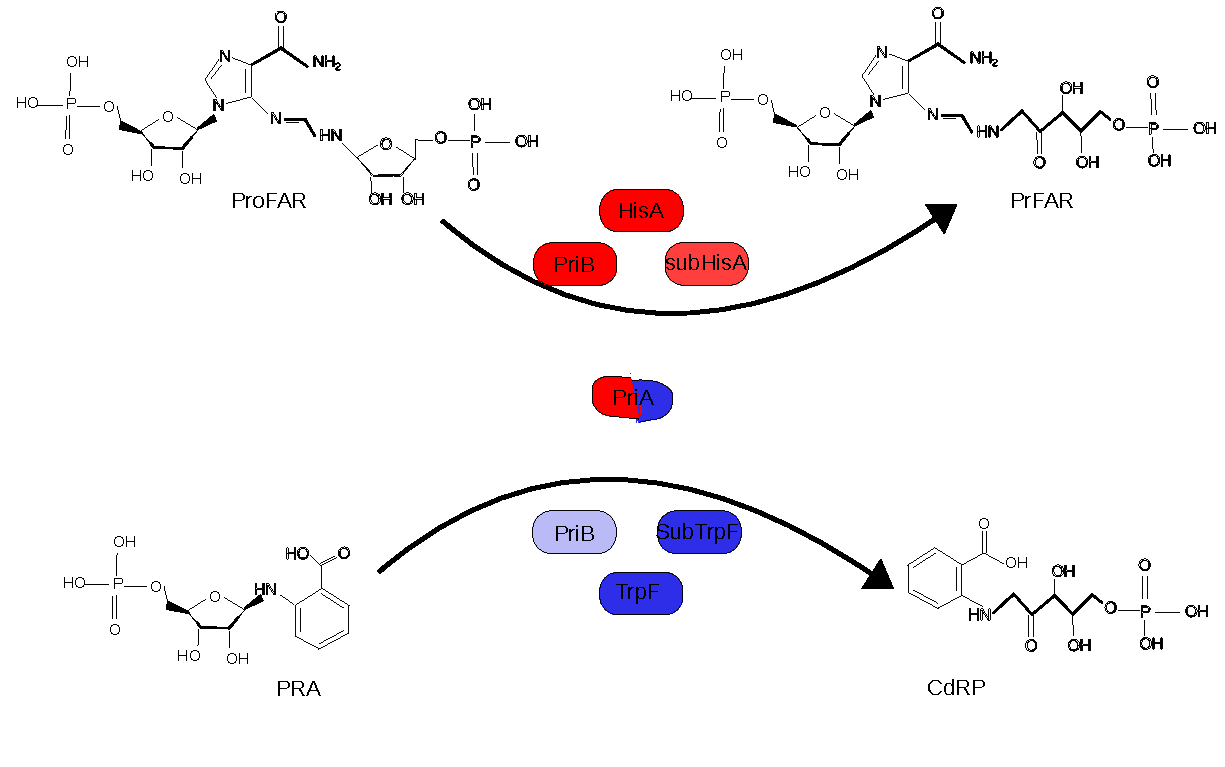
\includegraphics[angle = 0,scale = 0.6]{PriA.pdf}
  \caption[PriA isomeriza los sustratos PRA y ProFAR ]{\footnotesize{PriA cataliza la isomerización  de los sustratos nativos ProFAR y PRA. Convertir ProFAR es un paso de la síntesis de histidina catalizado por {hisA} en otros linajes bacterianos. Análogamente la isomerización de PRA es catalizada por {trpF} en otros linajes. En Actinobacteria PriA se ha subdidvidido en subfamilias. Entre ellas subHisA, que se ha subfunciónalizado a la función HisA, subTrpF que se ha subfunciónalizado a la función TrpF y finalmente PriB, que aún retiene la función TrpF pero con baja actividad catalítica.  }}
  \label{fig:priAFigure}
  \end{figure}
  
  Los operones \emph{his} y \emph{trp} de histidina
  {[}\protect\hyperlink{ref-fondi_evolution_2009}{44}{]} y triptofano
  {[}\protect\hyperlink{ref-merino_evolution_2008}{45}{]} respectivamente,
  participantes del metabolismo de amino ácidos, están ampliamente
  distribuidos en los organismos bacterianos. En Actinobacteria la familia
  promiscua PriA participa simultáneamente en ambas rutas biosintéticas
  \autoref{fig:priAFigure} desarrollando el equivalente a la función TrpF
  en la ruta de histidina y a la función TrpF en la ruta de triptofano.
  Como HisA isomeriza el sustrato ProFAR y como PRA isomeriza el sustrato
  PRA. Para su estudio se han generado datos bioquímicos
  \autoref{tab:cineticos}, genómicos y estructurales. En bacterias gram
  negativas están presentes los operones \emph{his} y \emph{trp} y en
  lugar de PriA existen dos familias HisA y TrpF. PriA es homóloga de HisA
  y adquirió la función de TrpF en Actinobacteria coincidentemente con que
  en este phylum \emph{trpF} está ausente de la mayoría de sus miembros.
  PriA se ha diversificado un conjunto de subfamilias en Actinobacteria,
  por ejemplo en \emph{Streptomyces}, existe la subfamilia PriB disminuye
  su actividad de TrpF debido a la presencia de una copia de \emph{trpF}
  en alguna parte del genoma
  {[}\protect\hyperlink{ref-verduzco-castro_co-occurrence_2016}{46}{]}. En
  otras Actinobacterias \emph{trpF} se pierde totalmente por ello PriA la
  familia homóloga de HisA, se vuelve promiscua
  {[}\protect\hyperlink{ref-baronagomez_occurrence_2003}{9}{]} realizando
  tanto la función química correspondiente a HisA como la de TrpF.
  Finalmente en la familia subHisA se pierde la función TrpF debido
  posiblemente a la ganancia del operón \emph{trp} completo
  {[}\protect\hyperlink{ref-noda-garcia_evolution_2013}{31}{]} y en la
  familia subtrpF se conserva solo a la función TrpF debido a la pérdida
  del operón \emph{his}
  {[}\protect\hyperlink{ref-juarez-vazquez_evolution_2017}{47}{]}. Existen
  al menos 43 familias de Actinobacteria sin explorar respecto a la
  funcionalidad de PriA. En la \autoref{tab:cineticos} se muestran la
  constantes catalíticas de PriA estimadas en diferentes organismos para
  estos dos sustratos.
  
  \clearpage    
  
  \begin{landscape}  
  Table: Capacidad catalítica respecto a PRA y ProFAR de miembros de la familia PriA \label{tab:cineticos} 
  $$
  \resizebox{\columnwidth}{!}{%
  \begin{tabular}{ l c r c c c c c c c l}
  \hline \\ [-1.5ex]
  Fuente  &Familia & HisA $in\hspace{.1cm}vivo$ &TrpF $in\hspace{.1cm}vivo$ & $K{cat}^{ProFAR}[M^{-1}s^{-1}]$ & $Km^{ProFAR}[\mu M]$& $\frac{K{cat}}{Km} ProFAR$ & $K{cat}^{PRA}[M^{-1}s^{-1}]$ & $Km^{PRA}[\mu M]$  &  $\frac{Kcat}{Km} PRA $  &Referencia  \\ [1ex]
  \hline \\ [-1.5ex]  
  \textit{Escherichia} \textit{coli}         & HisA &- &- & 1.6 & 4.9 & 3.1 & -   & -   & 0   & Henn-Sax 2002 \\ [1ex]  
  \textit{Escherichia}  \textit{coli}        &TrpF  &- &- &-    &-    &0    & 12.2& 34.5& 2.82& Sterner 1996 \\ [1ex]    
  \textit{Mycobacterium} \textit{tuberculosis} &PriA&-&-&19&0.23&12&21&3.6&0.17& Due 2011\\ [1ex]    
  \textit{Mycobacterium}  \textit{smegmatis} &PriA&*&*& 2.6 ± 0.5 & 0.85 $ \pm $ 0.04 &0.33& 7.9 $ \pm $  2.4& 3.1 $ \pm $0.43  &0.39& Verduzco-Castro 2016 \\ [1ex]   
  \textit{Streptomyces} \textit{globisporus}  &PriA&*&*& 4.2 ± 0.8& 0.74 ± 0.03 &0.18& 11 ± 1.0 & 3.8 ± 0.2 &0.34& Verduzco-Castro 2016\\ [1ex]  
  \textit{Streptomyces} \textit{coelicolor} &PriA&-&-& 3.6 ± 0.7 & 1.3 ± 0.2 &0.4& 5.0 ± 0.08 & 3.4 ± 0.09 &0.7& Noda-Garcia 2010\\ [1ex]   
  \textit{Streptomyces} \textit{ipomoeae}  &PriB&*&*& 3.8 ± 0.2 & 0.82 ± 0.02 &0.21& 60.8 ± 1.1&  8.25 ± 0.4&0.14& Verduzco-Castro 2016\\ [1ex]   
  \textit{Streptomyces} sp. Mg1  &PriB&*&*& 13.2 ± 3.4 &0.92 ± 0.19 &69&129.6 ± 34 &0.29 ± 0.04&0.0022&Verduzco-Castro 2016\\ [1ex]  
  \textit{Streptomyces} sp. C&PriB&*&*&11.4 ± 3.4 &2.53 ± 0.74 &0.22&149. 9 ± 29& 1.4 ± 0.12 &9&Verduzco-Castro 2016\\ [1ex]    
  \textit{Streptomyces} \textit{sviceus} &PriB&*&*&3.9 ± 0.89 &0.69 ± 0.04 &0.18&24.5 ± 4.0& 1.6 ± 0.29 &67&VVerduzco-Castro 2016\\ [1ex]   
  \textit{Corynebacterium} \textit{diphteriae} &subHisA&-&-&4.4 ± 0.5&2.6 ± 0.3&0.59&&&0& Noda-Garcia 2013\\ [1ex]    
  \textit{Corynebacterium} \textit{jeikeium} &PriA&-&-&2.3 ± 0.2&0.9 ± 0.08&0.39&5.1 ± 1.0&1.6 ± 0.16&0.31& Noda-Garcia 2013\\ [1ex]    
  \textit{Corynebacterium} \textit{striatum} &subHisA&-&-&6.9 ± 0.7&2.1 ± 0.5&0.3&&&0& Noda-Garcia 2013 \\ [1ex]    
  \textit{Corynebacterium} \textit{diphteriae}  L48I-F50L-T80S&subHisA&&&4.5 ± 1.5&0.6 ± 0.08&0.13&133 ± 10&0.05 ± 0.01&0.0004&NNoda-Garcia 2013\\ [1ex]    
  \textit{Actinomyces} \textit{urogenitalis} DSM 15434&PriB&*&*&2.1 ± 0.5 &1.8 ± 0.2 &0.9&26.3 ± 6.3& 0.37 ± 0.09 &14&Verduzco-Castro 2016\\ [1ex]   
  \textit{Actinomyces} \textit{odontolyticus}  ATCC 17982&subTrpF&&*&-&-&0&&&0.02&Juarez-Vazquez 2017\\ [1ex]    
  \textit{Actinomyces} \textit{oris} K20 BABV01&PriA&&&&&0.02&&&0.01&Juarez-Vazquez 2017\\ [1ex]    
  \textit{Actinomyces} sp. oral taxon 171 str. F0337&PriA&&&&&0.01&&&4&Juarez-Vazquez 2017\\ [1ex]    
  \textit{Actinomyces} sp. oral taxon 848 str. F0332&subTrpF&&*&-&-&0&&&0.0001&Juarez-Vazquez 2017\\ [1ex]    
  \textit{Actinomyces} \textit{urogenitalis} DSM 15434&PriA&&&&&0.01&&&0.02&Juarez-Vazquez 2017\\ [1ex]    
  \textit{Bifidobacterium} \textit{adolescentis} L2-32&PriA&*&*&&&0.2&&&0.1&Juarez-Vazquez 2017\\ [1ex]    
  \textit{Bifidobacterium} \textit{gallicum} DSM 20093 &PriA&*&*&&&0.1&&&0.04&Juarez-Vazquez 2017\\ [1ex]    
  \textit{Bifidobacterium} \textit{longum} ATCC 15697&PriA&*&*&&&0.1&&&0.3&Juarez-Vazquez 2017\\ [1ex]    
  Camera CAM1&Metagenoma&&&1.7 ± 0.1&0.3 ± 0.03&0.2&40 ± 7&3.5 ± 0.04&0.09&Noda-Garcia 2015\\ [1ex]    
  CAM1 A81G&Metagenoma&&&1.7 ± 0.2&0.1 ± 0.01&0.06&32.2 ± 1.7&1.9 ± 0.1&0.06&Noda-Garcia 2015\\ [1ex]    
  CAM1 A81S&Metagenoma&&&4.0 ± 0.9&0.2 ± 0.03&0.04&23.5 ± 6.5&0.5 ± 0.1&0.02&Noda-Garcia 2015\\ [1ex]    
  CAM2&Metagenoma&&&n.d.&n.d.&0&n.d.&n.d.&0&Noda-Garcia 2015\\ [1ex]    
  PriA Ancestral&Ancestral&&&9.4±1.6&0.3±0.009&0.03&4.3±0.4&0.6±0.02&0.13&Verduzco, Noda, sin publicar\\ [1ex]    
  PriA SubHisA&Ancestral&&&3.7±1.01&0.5±0.03&0.1&-&-&0&Verduzco, Noda, sin publicar\\ [1ex]    
  SubHisA Ancestral&Ancestral&&&6.3±0.7&0.15±0.03&0.02&-&-&0&Verduzco, Noda, sin publicar\\ [1ex]    
  SubHisA PriA&Ancestral&&&27.7±3.4&0.05±0.005&2&167.82&0.03±0.002&0.0001&Verduzco, Noda, sin publicar\\ [1ex]    
  \textit{Streptomyces} \textit{acidiscabies}&&0&0&163.6&0.1&&&&&Verduzco*\\ [1ex]  
  \textit{A} \textit{visco} &&&46&1.37&36&3.4&&&&Juárez*\\ [1ex]  
  \hline \\ [-1.5ex]
  \hline
  \end{tabular}
  }
  \label{tab:cineticos}  
  %}
  $$   
  \end{landscape}
  
  \normalsize
  
  \subsection{Relacion del pangenoma con la promiscuidad
  enzimatica}\label{relacion-del-pangenoma-con-la-promiscuidad-enzimatica}
  
  El pangenoma es el contenido génico total de un linaje taxonómico. Las
  familias génicas de un pangenoma pueden clasificarse según su frecuencia
  de presencia/ausencia en cada genoma del linaje. De acuerdo a esta
  clasificación los principales grupos de familias génicas en un pangenoma
  son el \emph{core}, el \emph{shell} y el \emph{cloud} también conocido
  como \emph{dispensable} o \emph{accesory genome}. El \emph{core genome}
  es el conjunto de familias con presencia en todos los genomas del
  linaje. Por ejemplo, tanto la secuencia de la subunidad 16s de rRNA así
  como los diversos genes ribosomales suelen estar en el \emph{core} de la
  gran mayoría de linajes bacterianos. El \emph{shell genome} es el grupo
  de familias presentes en la mayoría de los genomas pero no en todos. En
  el \emph{shell} se ubican por ejemplo familias que estaban en el
  \emph{core genome} pero que algunas bacterias del linaje sufrieron una
  dinámica de pérdida génica. Mientras que el \emph{cloud genome} o
  \emph{dispensable genome} es aquel grupo de familias que sólo ocurre en
  unos cuantos genomas del linaje.
  
  En el Dominio Bacteria se estima que alrededor de 200 familias de
  secuencias están altamente conservadas. Si bien no están en el \(core\),
  estas secuencias están compartidas por 90\% de los genomas
  {[}\protect\hyperlink{ref-halachev_calculating_2011}{48}{]}. El
  \emph{core} depende de los genomas seleccionados, entre menos amplio sea
  el rango filogenético elegido mayor será el tamaño del \(core\). Dada su
  conservación el \(core~genome\) puede utilizarse para trazar mejores
  relaciones filogenéticas que las obtenidas con el uso exclusivo de
  marcadores como la subunidad 16s del RNA ribosomal o la proteína RpoB.
  El \emph{dispensable} y el \emph{shell genome} son juntos el conjunto
  complemento del \emph{core genome}, es decir todas aquellas secuencias
  que están ausentes de uno o más organismos del grupo y por lo tanto no
  son necesarias para todos, sino sólo posiblemente para el organismo que
  las posee. Como en estos grupos la presión de selección está relajada
  respecto al \emph{core-genome}
  {[}\protect\hyperlink{ref-firn_darwinian_2009}{18}{]} es el conjunto
  ideal donde la plasticidad genómica tiene facilidades para
  desarrollarse.
  
  Esta idea puede restringirse a subsistemas metabólicos para identificar
  genes cuyas enzimas están en proceso de cambio de función química, por
  ejemplo, en este trabajo se encontró que el gen \emph{trpF} está
  presente en solo 49 de 290 genomas analizados del género
  \emph{Streptomyces}. Por lo que \emph{trpF} se encuentra en el
  \emph{dispensable genome} de este género taxonómico, posiblemente
  adquiriendo una nueva función
  {[}\protect\hyperlink{ref-ma_unconventional_2013}{41}{]}. Para evitar
  problemas técnicos del cálculo del pangenoma existen modelos de medición
  de variabilidad del genómica entre especies bacterianas
  {[}\protect\hyperlink{ref-kislyuk_genomic_2011}{49}{]}.
  
  \subsection{Modelos bioinformaticos de
  promiscuidad}\label{modelos-bioinformaticos-de-promiscuidad}
  
  Con el fin de reducir la inversión en el proceso de experimentación, se
  han implementado algoritmos computacionales para predecir promiscuidad
  enzimática {[}\protect\hyperlink{ref-carbonell_molecular_2010}{28}{]}.
  Estos procedimientos cuentan con un conjunto de aprendizaje, unos
  descriptores del conjunto, una fase de ajuste de parámetros y finalmente
  una predicción. En 2010, Carbonell propone un algoritmo de soporte
  vectorial basado en subsecuencias de distinto tamaño que llama huellas
  moleculares. En este trabajo aplicado sobre 500,000 proteínas reportadas
  en la enciclopedia de Kyoto de genes y genomas (KEGG) se reporta 85\% de
  éxito en detección de enzimas promiscuas anotadas en KEGG. En 2012,
  Cheng compara los métodos de random forest y soporte vectorial en 6799
  proteínas provenientes de la base de datos \emph{Universal Protein
  Resource} (UniProt). Las enzimas son descritas con subsecuencias de
  aminoácidos incorporando además características biofísicas como
  polaridad. Se utiliza como grupo de control a familias de enzimas donde
  nunca se ha reportado una enzima promiscua.
  
  Un aspecto no considerado en estos métodos es que hay familias de
  enzimas con alta identidad de secuencia entre sus miembros, con cambios
  bruscos en promiscuidad, debidos por ejemplo a la dinámica genómica
  {[}\protect\hyperlink{ref-noda-garcia_evolution_2013}{31}{]}, o bien que
  ortólogos de la misma familia enzimática pueden variar en su grado de
  promiscuidad {[}\protect\hyperlink{ref-bloom_neutral_2007}{15}{]}. Esta
  característica dificulta considerar solo la secuencia conlleve a buenos
  predictores de promiscuidad. Obtener una predicción positiva utilizando
  los modelos existentes significa que dada esa secuencia, en su familia
  se conoce previamente un elemento promiscuo y que además sus
  subsecuencias de cierto tamaño son suficientemente similares. Estos
  enfoques no pueden predecir \emph{de novo}, en familias donde la
  promiscuidad no ha sido previamente detectada experimentalmente, pues no
  consideran aspectos evolutivos ni mecanísticos de las enzimas.
  
  Otra limitante a los enfoques descritos es que mezclan en su conjunto de
  entrenamiento fenómenos distintos de promiscuidad. Cheng p.~g. incluye
  enzimas \emph{moonlight} que si bien poseen funciones adicionales a la
  catalización, son distantes a las enzimas promiscuas
  {[}\protect\hyperlink{ref-copley_enzymes_2003}{6}{]}. Además en ambos
  casos mezclan en el mismo conjunto enzimas bacterianas y eucariotas, con
  lo que si existía una huella basada en secuencia entonces ésta puede
  diluirse por la gran distancia taxonómica entre estos grupos.
  
  \subsection{Promiscuidad in vitro y promiscuidad in
  vivo}\label{promiscuidad-in-vitro-y-promiscuidad-in-vivo}
  
  La ganancia de promiscuidad no sólo puede entenderse como la capacidad
  de convertir más sustratos
  {[}\protect\hyperlink{ref-carbonell_molecular_2010}{28}{]}, sino también
  como la mejora de la capacidad catalítica respecto a ellos. El I-index
  {[}\protect\hyperlink{ref-nath_quantitative_2008}{16}{]}, está definido
  como un rango de valores entre 0 y 1 que tiende a 1 entre más parecida
  sea la actividad de la enzima sobre distintos sustratos, la capacidad
  catalítica es medida en términos del cociente de \emph{Michaelis -
  Menten} \(\frac{K_{cat}}{K_m}\). El índice ha sido utilizado para
  predecir la afinidad por sustrato del citocromo P450
  {[}\protect\hyperlink{ref-nath_quantifying_2010}{25}{]}. Una limitante
  del índice \(I\) es que se deben conocer los sustratos a los que la
  enzima es afín; sin embargo se puede sospechar que una enzima ha ganado
  promiscuidad aun sin conocer sus potenciales sustratos. Otro punto a
  señalar es que las variables \(K_{cat}\),\(K_m\) son mediciones
  realizadas \emph{in vitro} y no se consideran todos los sustratos
  presentes \emph{in vivo}. Para solventar esta dificultad e investigar
  variaciones de sustratos nativos se pueden buscar productos similares a
  los ya conocidos por medio de análisis bioinformáticos o metabólicos
  {[}\protect\hyperlink{ref-nesvizhskii_analysis_2007}{52}{]} como los
  empleados en la detección de rutas no conservadas en la biosíntesis de
  productos naturales
  {[}\protect\hyperlink{ref-medema_computational_2015}{53}{]}. En
  particular para este fin se ha utilizado espectroscopia de masas
  \(\frac{MS}{MS}\),
  {[}\protect\hyperlink{ref-nesvizhskii_analysis_2007}{52}{]} combinada
  con molecular networking para identificar productos similares
  {[}\protect\hyperlink{ref-yang_molecular_2013}{55}{]}
  
  \subsection{El papel de la dinámica molecular en la
  promiscuidad}\label{el-papel-de-la-dinamica-molecular-en-la-promiscuidad}
  
  La mayoría de las estructuras tridimensionales de proteína se han
  obtenido por cristalización de rayos X. Aunque mucho se ha hablado de la
  relación estructura función, al cristalizar se obtienen estados
  conformacionales homogéneos, que bien pueden no ser la única
  conformación que adopta la proteína en solución
  {[}\protect\hyperlink{ref-james_conformational_2003}{57}{]}. En
  particular en el problema de promiscuidad, se ha observado que la
  variación funcional no queda obviamente reflejada en la variación
  estructural, lo que sugiere un rol significativo para la dinámica
  molecular {[}\protect\hyperlink{ref-parisi_conformational_2015}{58}{]}.
  Se postula que un aspecto de la dinámica molecular relevante para la
  diversificación de especificidad por sustrato es el numero de
  confórmeros {[}\protect\hyperlink{ref-javier_zea_protein_2013}{59}{]}.
  Por ejemplo, en la actinobacteria \emph{Corynebacterium diphtheriae}
  parece que el contexto genómico correlaciona con pérdida de promiscuidad
  de PriA ya que al poseer el genoma una copia de \emph{trpF}, la enzima
  perdió esta función química conservando solo la función EC 5.3.1.16
  correspondiente a la ruta de histidina. Esta sub-funcionalización se
  refleja en la pérdida de estados conformacionales cambiando desde un
  estado en \emph{C. diphtheriae} hasta 4 presentes en la dinámica de PriA
  de \_ M. tuberculosis\_
  {[}\protect\hyperlink{ref-noda-garcia_evolution_2013}{31}{]}.
  
  Las regiones rígidas de una enzima proporcionan orientación adecuada con
  respecto a los grupos catalíticos, mientras que las regiones flexibles
  permiten al sitio activo adaptarse a los sustratos con diferentes formas
  y tamaños {[}\protect\hyperlink{ref-copley_enzymes_2003}{6}{]}. Esta
  consideración sugiere que la flexibilidad del sitio activo es otra
  característica de la dinámica molecular a considerar para obtener
  información de la capacidad de ligación de una enzima a distintos
  sustratos
  {[}\protect\hyperlink{ref-gatti-lafranconi_flexibility_2013}{60}{]}.
  Recientemente el índice de flexibilidad dinámica (dfi) se utilizó como
  una medida cuantitativa basado en la respuesta a perturbaciones de amino
  ácidos (PRS). Este indice se incrementó en regiones cercanas al sitio
  activo de beta lactamasas promiscuas respecto al correspondiente dfi de
  \(\noindent\beta\) -lactamasas especialistas existentes
  {[}\protect\hyperlink{ref-zou_evolution_2015}{17}{]}.
  
  \subsection{Modelo biológico: la diversidad de
  Actinobacteria}\label{modelo-biologico-la-diversidad-de-actinobacteria}
  
  Al escoger un conjunto acotado para investigar familias de enzimas
  promiscuas se debe recordar que la funcionalidad es jerárquica por lo
  que para mejorar la anotación, es deseable reflejar el proceso evolutivo
  y restringirse a un grupo de organismos taxonómicamente relacionados
  {[}\protect\hyperlink{ref-cruz-morales_phylogenomic_2016}{61}{]}.
  Actinobacteria es un phylum que posee promiscuidad tanto en el
  metabolismo periférico como en el core metabólico. Entre datos públicos
  (NCBI) y privados están disponibles en 2014 alrededor de 1200 genomas no
  redundantes de especies de Actinobacteria. Como punto de partida, se han
  estudiado las relaciones filogenéticas y grupos de ortología
  {[}\protect\hyperlink{ref-li_orthomcl_2003}{62}{]}, en particular en
  Actinobacteria para identificar relaciones entre las familias del
  phylum, se han obtenido árboles multilocus de entre 100 y 157 genomas
  {[}\protect\hyperlink{ref-gao_phylogenetic_2012}{64}{]}. Estos estudios
  sugieren como separar los genomas disponibles para hacer el cálculo de
  grupos de ortología. Finalmente, se han realizado estudios de
  plasticidad genómica en \emph{Streptomyces} considerando 5 y 17
  organismos de los 300 genomas disponibles en la actualidad
  {[}\protect\hyperlink{ref-zhou_genome_2012}{66}{]} donde reportan
  respectivamente 2,018 familias en el \emph{core genome} y 32,574 en el
  pangenoma. Además de Actinobacteria, otros linajes con riqueza
  metabólica conocida en metabolitos secundarios como Cianobacteria y
  \(Pseudomonas\) también serán considerados en este trabajo. Finalmente
  un dominio desconocido pero del que comienza a haber genomas disponibles
  \textasciitilde{}800 genomas públicos en NCBI en 2016. Todos estos
  linajes pueden ser considerados en la búsqueda de variación de
  promiscuidad.
  
  \subsection{Modelo metabolico biosintesis de
  aminoacidos.}\label{modelo-metabolico-biosintesis-de-aminoacidos.}
  
  Al hacer el cálculo vemos que \emph{Streptomyces}, un genero del phylum
  Actinobacteria cuenta en su genoma con un promedio de 8316 secuencias
  codificantes según la especie. Gran parte de estas secuencias pueden ser
  agrupadas en subsistemas metabólicos como metabolismo de carbohidratos o
  de lípidos; de estos subsistemas uno de los más amplios es el
  metabolismo de aminoácidos con entre 429 y 910 secuencias según el
  organismo. La síntesis de amino ácidos es un subsistema presente en
  todas las especies pero con suficientes variaciones que permiten hacer
  observaciones evolutivas. En un gran número de Actinobacterias las rutas
  de histidina y triptofano de 7 y 11 pasos respectivamente convergen en
  una enzima funcional llamada PriA, que realiza tanto la función de HisA
  como la de TrpF
  {[}\protect\hyperlink{ref-baronagomez_occurrence_2003}{9}{]}. La
  cantidad de familias en el subsistema de metabolismo de aminoácidos, su
  variabilidad, su conservación entre distintos grupos taxonómicos y la
  existencia de estos ejemplos en Actinobacteria posicionan al metabolismo
  de amino ácidos como un buen punto de partida para la búsqueda de
  promiscuidad tanto de familias promiscuas como de miembros promiscuos de
  las mismas.
  
  En las cuatro décadas de estudio de la promiscuidad enzimática, hemos
  aprendido que es un fenómeno distribuido en distintos subsistemas
  metabólicos {[}\protect\hyperlink{ref-nam_network_2012}{2}{]} y que su
  existencia puede deberse tanto al desarrollo de nuevas funciones para
  fines adaptativos {[}\protect\hyperlink{ref-jensen_enzyme_1976}{1}{]},
  como al rescate de una función perdida
  {[}\protect\hyperlink{ref-patrick_multicopy_2007}{3}{]}. Por ello la
  dinámica de pérdida y ganancia de genes asociada al contexto genómico en
  bacterias se relaciona con cambio en la función enzimática
  {[}\protect\hyperlink{ref-zhao_discovery_2013}{68}{]}. Precisando,
  respecto a la ganancia de genes, se postula que la funcionalidad precede
  la duplicación {[}\protect\hyperlink{ref-hughes_evolution_1994}{69}{]}.
  Lo que implica que dada una duplicación muy posiblemente previamente la
  promiscuidad estuvo presente.
  {[}\protect\hyperlink{ref-gerlt_divergent_2001}{70}{]}.
  
  Se han desarrollado técnicas bioquímicas y metabólicas de medición
  {[}\protect\hyperlink{ref-nath_quantitative_2008}{16}{]}, así como
  algoritmos computacionales de predicción de promiscuidad
  {[}\protect\hyperlink{ref-carbonell_molecular_2010}{28}{]}. Un aspecto a
  mejorar dentro del modelado es la restricción del conjunto de estudio a
  un grupo taxonómico tan reducido que exista congruencia en las familias
  de ortología y a la vez tan amplio que permita observar efectos
  evolutivos; el phylum Actinobacteria ha probado tener ejemplos de
  promiscuidad. Si bien la secuencia no ha sido suficiente para la
  correcta predicción de promiscuidad
  {[}\protect\hyperlink{ref-verdel-aranda_molecular_2015}{32}{]}, es
  posible que dentro de las técnicas computacionales, incorporar
  consideraciones evolutivas o bien flexibilidad durante la dinámica
  molecular nos proporcionen sugerencias sobre promiscuidad de los
  miembros de una familia
  {[}\protect\hyperlink{ref-james_conformational_2003}{57}{]}.
  
  \section{Modelos computacionales}\label{modelos-computacionales}
  
  Para desarrollar herramientas bioinformáticas relacionadas al estudio de
  la promiscuidad se adoptó el enfoque de los contenedores
  bioinformáticos, todo el código fue depositado y documentado en GitHub y
  distribuido a través de un contenedor Docker siguiendo las
  especificaciones generales de desarrollo de biocontenedores
  {[}\protect\hyperlink{ref-schulz_use_2016}{72}{]}.
  
  \clearpage  
  
  \chapter*{Antecedentes}\label{antecedentes}
  \addcontentsline{toc}{chapter}{Antecedentes}
  
  \begin{figure}[h!tbp]
  \centering
  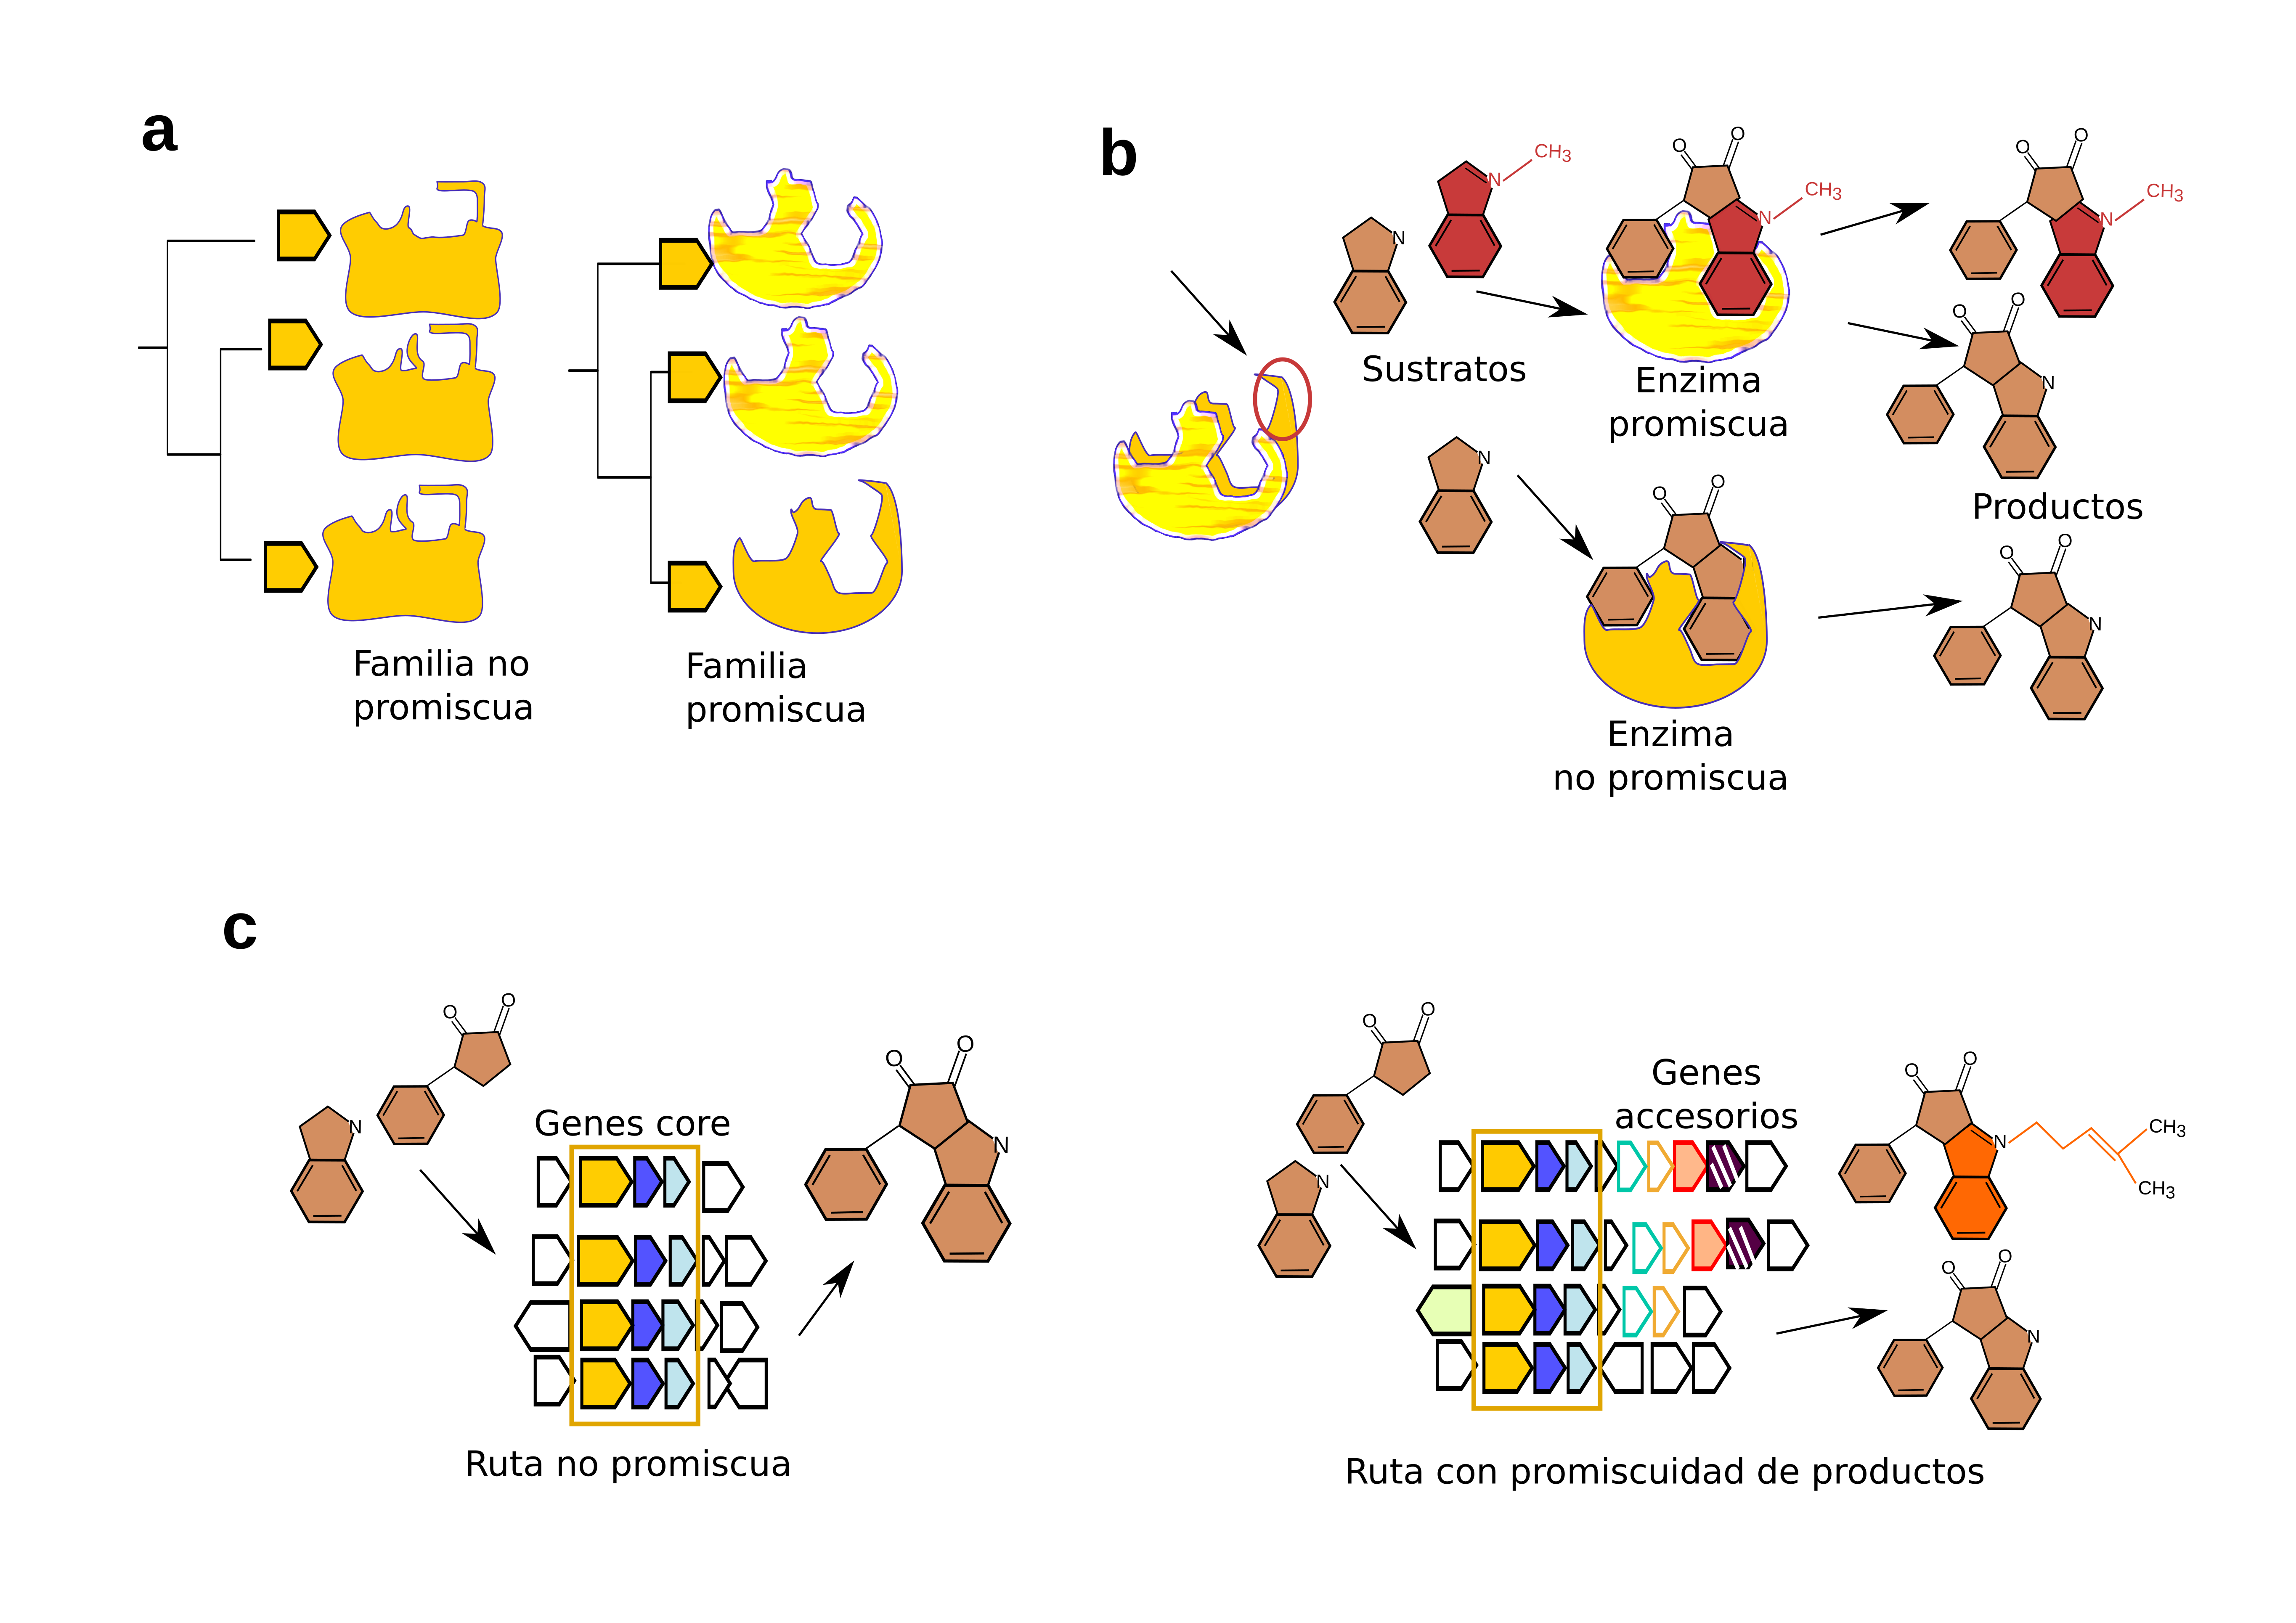
\includegraphics[angle = 0,scale = 0.6]{chapter0/NivelesPromiscuidad.png}
  \caption[La promiscuidad puede entenderse a distintos niveles metabólicos: enzima, familia enzimática y ruta biosintética]{\normalsize{La promiscuidad puede entenderse a distintos niveles metabólicos: enzima, familia enzimática y ruta biosintética}}
  \label{fig:niveles}
  \end{figure}
  
  \section{La promiscuidad puede abordarse a distintos niveles incluyendo
  enzima, familia y ruta de
  metabólica.}\label{la-promiscuidad-puede-abordarse-a-distintos-niveles-incluyendo-enzima-familia-y-ruta-de-metabolica.}
  
  Si se entiende a la promiscuidad como funciones alternativas de alguna
  unidad molecular, puede observarse promiscuidad a distintos niveles:
  desde un mismo gen que presenta splicing alternativo, una misma enzima
  con funciones alternativas, o bien una familia enzimática donde al menos
  algunos homólogos codifican enzimas promiscuas
  {[}\protect\hyperlink{ref-nobeli_protein_2009}{23}{]}. Existen también
  rutas que generan productos metabólicos alternativos
  {[}\protect\hyperlink{ref-lamble_archaea_promiscuou_pathways_2003}{74}{]},
  si se considera como la unidad de estudio a una ruta biosintética
  podemos generalizar la noción de promiscuidad al concepto de rutas
  promiscuas. La \autoref{fig:niveles} muestra tres niveles en los que se
  puede estudiar la promiscuidad: i) Distinguiendo familias de enzimas
  promiscuas de familias especialistas, ii) Distinguiendo enzimas
  específicas de enzimas especialistas en una familia enzimática promiscua
  y finalmente iii) encontrando promiscuidad en rutas de metabolismo
  especializado.
  
  Para clarificar la diferencia entre identificar familias promiscuas y
  miembro de familias promiscua se propone el siguiente ejemplo: PriA en
  Actinobacteria y HisA en enterobacteria son ambas familias que
  isomerizan ProFAR en la ruta de síntesis de histidina pero solo la
  familia PriA es promiscua pues puede además isomerizar el sustrato PRA
  durante la síntesis de triptofano
  {[}\protect\hyperlink{ref-baronagomez_occurrence_2003}{9}{]}. Sin
  embargo dentro de Actinobacteria, existen miembros no promiscuos de
  PriA. Cinéticas \emph{in vitro} han mostrado que en algunas especies del
  género \emph{Actinomyces} los homólogos de \emph{priA} codifican para
  enzimas monofuncionales en alguno de los dos sustratos
  {[}\protect\hyperlink{ref-juarez-vazquez_evolution_2017}{47}{]}. Así
  pues dentro de una familia promiscua no todos los miembros tienen esta
  propiedad {[}\protect\hyperlink{ref-bloom_neutral_2007}{15}{]}. En este
  trabajo se buscará encontrar marcas de promiscuidad a nivel familia,
  enzima y ruta biosintética en el metabolismo especializado.
  
  \begin{figure}[h!tbp]
  \centering
  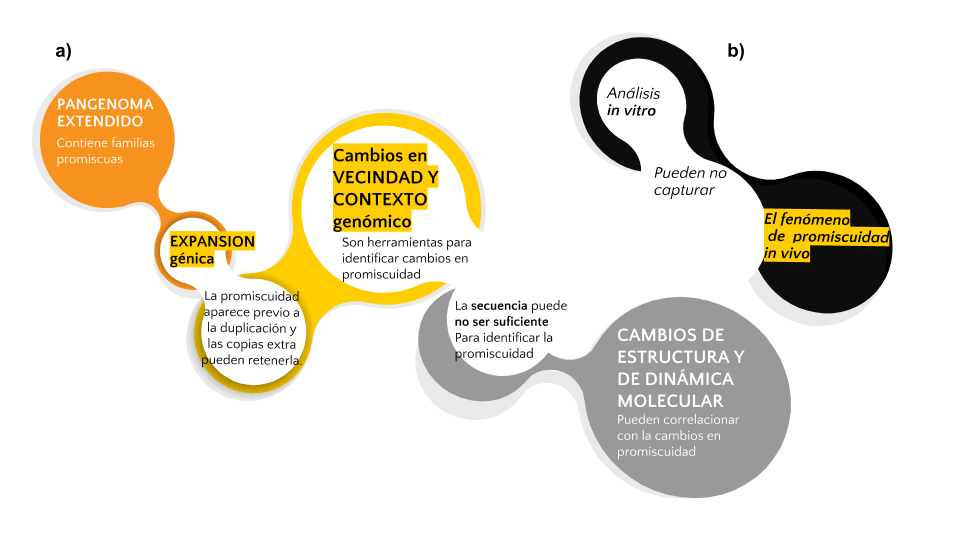
\includegraphics[angle = 0,scale = 0.5]{chapter0/AntecedentesConceptuales.png}
  \caption[Antecedentes conceptuales de promiscuidad metabólica]{\normalsize{Antecedentes conceptuales de promiscuidad metabólica}}
  \label{fig:Antecedentes}
  \end{figure}
  
  \section{Antecedentes conceptuales}\label{antecedentes-conceptuales}
  
  Algunos autores han intentado identificar enzimas promiscuas mediante
  aprendizaje máquina utilizando únicamente la secuencia de aminoácidos.
  Estos enfoques no han distiguido entre los problemas identificación de
  familias promiscuas e identificación a nivel de enzima
  {[}\protect\hyperlink{ref-carbonell_molecular_2010}{28}{]}. Hasta ahora
  utilizar únicamente la información de la secuencia de aminoácidos no ha
  sido suficiente para identificar una familia promiscua sin conocer
  previamente al menos un miembro promiscuo de ella. Por otra parte,
  diferenciar la promiscuidad a nivel de enzima una vez que se conoce una
  familia promiscua se dificulta cuando la identidad de secuencia es alta.
  Tal es el caso de las PriA que han perdido la promiscuidad en algunos
  miembros del género \emph{Actinomyces}
  {[}\protect\hyperlink{ref-juarez-vazquez_evolution_2017}{47}{]}. En este
  caso el establecimiento de las filogenia de los miembros del género
  permitió entender la distribución de la
  
  Para mejorar nuestro entendimiento del fenómeno de promiscuidad, además
  de la comparación de secuencias es necesario integrar otros elementos al
  análisis,\autoref{fig:Antecedentes}. Es difícil medir la promiscuidad en
  términos absolutos, por ejemplo, no se puede aseverar que una enzima es
  ``no promiscua'' sin haber previamente descartado a todos los posibles
  sustratos del universo químico. Además incluso enzimas que resultan no
  promiscuas en análisis \emph{in vitro} resulta que sí son promiscuas al
  examinarlas \emph{in vivo}
  {[}\protect\hyperlink{ref-noda_tesis_2012}{75}{]}. Sin embargo debido a
  que al adquirir una nueva función existe un umbral donde la función
  ancestral es conservada, es plausible intentar transformar el problema
  de ``encontrar promiscuidad'' al de ``encontrar cambios en
  promiscuidad'' al relacionar estos cambios con las huellas que dejan los
  cambios funcionales
  {[}\protect\hyperlink{ref-soskine_mutational_2010}{43}{]}. Entre los
  elementos relevantes que correlacionan con la adquisición de una función
  alternativa se encuentran además de divergencia de secuencia, diversidad
  en vecindad
  genómica{[}\protect\hyperlink{ref-zhao__function_prediction_neighbourhood_2014}{76}{]},
  la pérdida o ganancia de
  genes{[}\protect\hyperlink{ref-juarez-vazquez_evolution_2017}{47}{]},
  las expansiones génicas, i.e.~el crecimiento del pangenoma dentro de un
  grupo taxonómico
  {[}\protect\hyperlink{ref-martinez-nunez_lifestyle_2015}{37}{]} y
  finalmente cambios estructurales o de flexibilidad durante la dinámica
  molecular{[}\protect\hyperlink{ref-zou_evolution_2015}{17}{]}. Estos
  elementos tienen en común que reflejan un cambio en alguna propiedad
  genómica o biofísica observable en el registro evolutivo, de lo que se
  deriva que el buscar cambios en la promiscuidad de una enzima, familia o
  ruta, resulta más factible por ahora que la búsqueda intrínseca de
  promiscuidad.
  
  Debido a la abundancia de datos genómicos los primeros capítulos de este
  trabajo se centran en encontrar variaciones en secuencia, distribución
  del pangenoma, y vecindades genómicas para encontrar candidatos de
  familias, enzimas y rutas promiscuas.\\
  
  \section{El establecimiento de un marco de conservación permite
  distinguir
  cambios}\label{el-establecimiento-de-un-marco-de-conservacion-permite-distinguir-cambios}
  
  La función de una enzima es un concepto jerárquico, dependiente de la
  filogenia de un organismo
  {[}\protect\hyperlink{ref-szklarczyk_string_2015}{77}{]}. Por ello, para
  poder encontrar marcas de cambio funcional, por ejemplo diferencias en
  número de copias de una familia, primero es importante trabajar en la
  construcción de un marco filogenético consistente que permita ordenar
  inclusive organismos de la misma especie. La dificultad de esta tarea
  consiste en que si los organismos que se desea ordenar son muy cercanos,
  marcadores clásicos como el gen de 16s son también muy parecidos en
  secuencia y no permiten resolver las relaciones entre ellos. Este caso
  dificultó la construcción de un árbol filogenético de \emph{Actinomyces}
  y con ello se imposibilitaba encontrar patrones en la matriz de
  presencia / ausencia de genes
  {[}\protect\hyperlink{ref-juarez-vazquez_evolution_2017}{47}{]}.
  
  Para solventar la falta de resolución de genes individuales en
  organismos cercanos puede utilizarse el conjunto de todos los genes
  comunes en un linaje. Este conjunto es conocido como el \emph{core
  genome}. Se han desarrollado herramientas bioinformáticas para este
  problema, por ejemplo phyloPhlan
  {[}\protect\hyperlink{ref-segata_phylophlan_2013}{78}{]} fija 400 genes
  comunes en bacteria y trata de localizarlos dado un conjunto de genomas
  sin importar su linaje. Este enfoque enfrenta que el contenido génico de
  genomas procariontes suele ser muy variable debido a mecanismos como
  transferencia horizontal y duplicación génica
  {[}\protect\hyperlink{ref-land_insights_2015}{79}{]}. Esta variabilidad
  puede impedir encontrar muchos de estos 400 genes en un cierto linaje.
  Entre organismos de la misma especie pueden suceder fenómenos como que
  el \emph{core} siempre se reduzca al aumentar un nuevo genoma y que el
  conjunto total de familias geńicas (pangenoma) siempre aumente. Aunado a
  esta observación biológica están también las limitaciones técnicas, hay
  genes que no aparecen en un genóma porque este fue mal secuenciado o
  ensamblado y por lo tanto estos genes disminuyen el tamaño del core.
  Para distinguir cambios en el contenido génico en un linaje de
  organismos es útil establecer primero un orden entre los genomas del
  linaje a analizar. Para ello, un camino que generaliza la propuesta de
  phyloPhlan es localizar los genes del \emph{core} exclusivos de cada
  grupo de genomas. Al momento existe publicada \emph{metaphor}, una
  herramienta de selección de ortólogos
  {[}\protect\hyperlink{ref-van_der_veen_metaphor_2014}{81}{]} pero al
  comenzar este trabajo no existía un método disponible para ello. Por
  ello el capítulo uno de esta tesis habla del desarrollo de Orthocore,
  que obtiene los genes del \emph{core} y además los concatena y entrega
  un árbol filogenético.
  
  \section{La genómica comparativa como herramienta en la distinción de
  familias y enzimas promiscuas que participan en el metabolismo
  especializado.}\label{la-genomica-comparativa-como-herramienta-en-la-distincion-de-familias-y-enzimas-promiscuas-que-participan-en-el-metabolismo-especializado.}
  
  Una parte del metabolismo especializado está compuesta por familias
  enzimáticas que evolucionaron de rutas de metabolismo central
  {[}\protect\hyperlink{ref-caetano-anolles_origin_metabolism_2009}{82}{]}.
  En las familias expandidas, ya sea por duplicación o por transferencia
  horizontal, las expansiones pueden retener la función química de las
  rutas centrales
  {[}\protect\hyperlink{ref-schniete_expanding_2018}{83}{]}, así como
  también la función alternativa suele estár presente presente aún a bajos
  niveles antes de la divergencia o duplicación
  {[}\protect\hyperlink{ref-soskine_mutational_2010}{43}{]}. Por tanto las
  familias con expansiones en un linaje son candidatas a ser familias
  promiscuas en él. Se ha notado que en el linaje en que una familia
  enzimática es promiscua hay una zona de cambio en promiscuidad
  {[}\protect\hyperlink{ref-noda-garcia_insights_2015}{50}{]}, Las
  expansiones de rutas centrales que participan en la síntesis de
  productos naturales son candidatos a presentar cambios en promiscuidad
  tanto a nivel familia como a nivel enzima. Por ello la observación de la
  retención de función ancestral al aparecer una función alternativa
  proporciona una zona favorable para la búsqueda de promiscuidad a nivel
  de enzima. En la familia existirá un gradiente de promiscuidad donde las
  más cercanas a la zona de duplicación o divergencia tienen más
  indicaciones de tener un cambio en promiscuidad que las más conservadas
  y cercanas al metabolismo central. Estas copias extra son candidatas a
  pertenecer a rutas de metabolismo especializado.
  
  Como prueba de concepto esta idea de minar genomas incorporando
  información evolutiva permitió la identificacion de la biosíntesis de
  arsenolipidos
  {[}\protect\hyperlink{ref-cruz-morales_phylogenomic_2016}{61}{]}. En
  este trabajo se desarrollo la idea de EvoMining, un método de minería
  genómica que permite localizar familias enzimáticas con copias extra en
  su linaje genómico que además presentaran marcas de reclutamiento a
  metabolismo especializado. La aplicación de las ideas de EvoMining
  llevaron a identificar una expansión en el número de copias de la enzima
  AroA en Actinobacteria. Se demostró experimentalmente que la copia
  secundaria era parte de un cluster de síntesis de arsenolípidos,
  \autoref{fig:niveles} . Es interesante remarcar que las funciones tanto
  primaria como secundaria son similares, lo que cambia es la
  especificidad de sustrato en cada copia. En la copia primaria el
  sustrato tiene un átomo de fósforo, en la secundaria uno de arsénico.
  Otros genes del cluster biosintético también parecen ser expansiones de
  familias del metabolismo central. Este descubrimiento se realizó con la
  primera versión de EvoMining que contó con 200 genomas de Actinobacteria
  {[}\protect\hyperlink{ref-cruz-morales_phylogenomic_2016}{61}{]}, una
  base de datos de secuencias de enzimas de productos naturales y otra
  base de datos de secuencias de enzimas de rutas centrales curada a mano.
  En esta primera versión quedaba pendiente poder utilizar EvoMining como
  plataforma de exploración de linajes personalizables con genomas
  provistos por el usuario, así como sistematizar la información del
  conjunto de enzimas consideradas como partícipes de BGC de productos
  naturales.
  
  \begin{figure}[h!tbp]
  \centering
  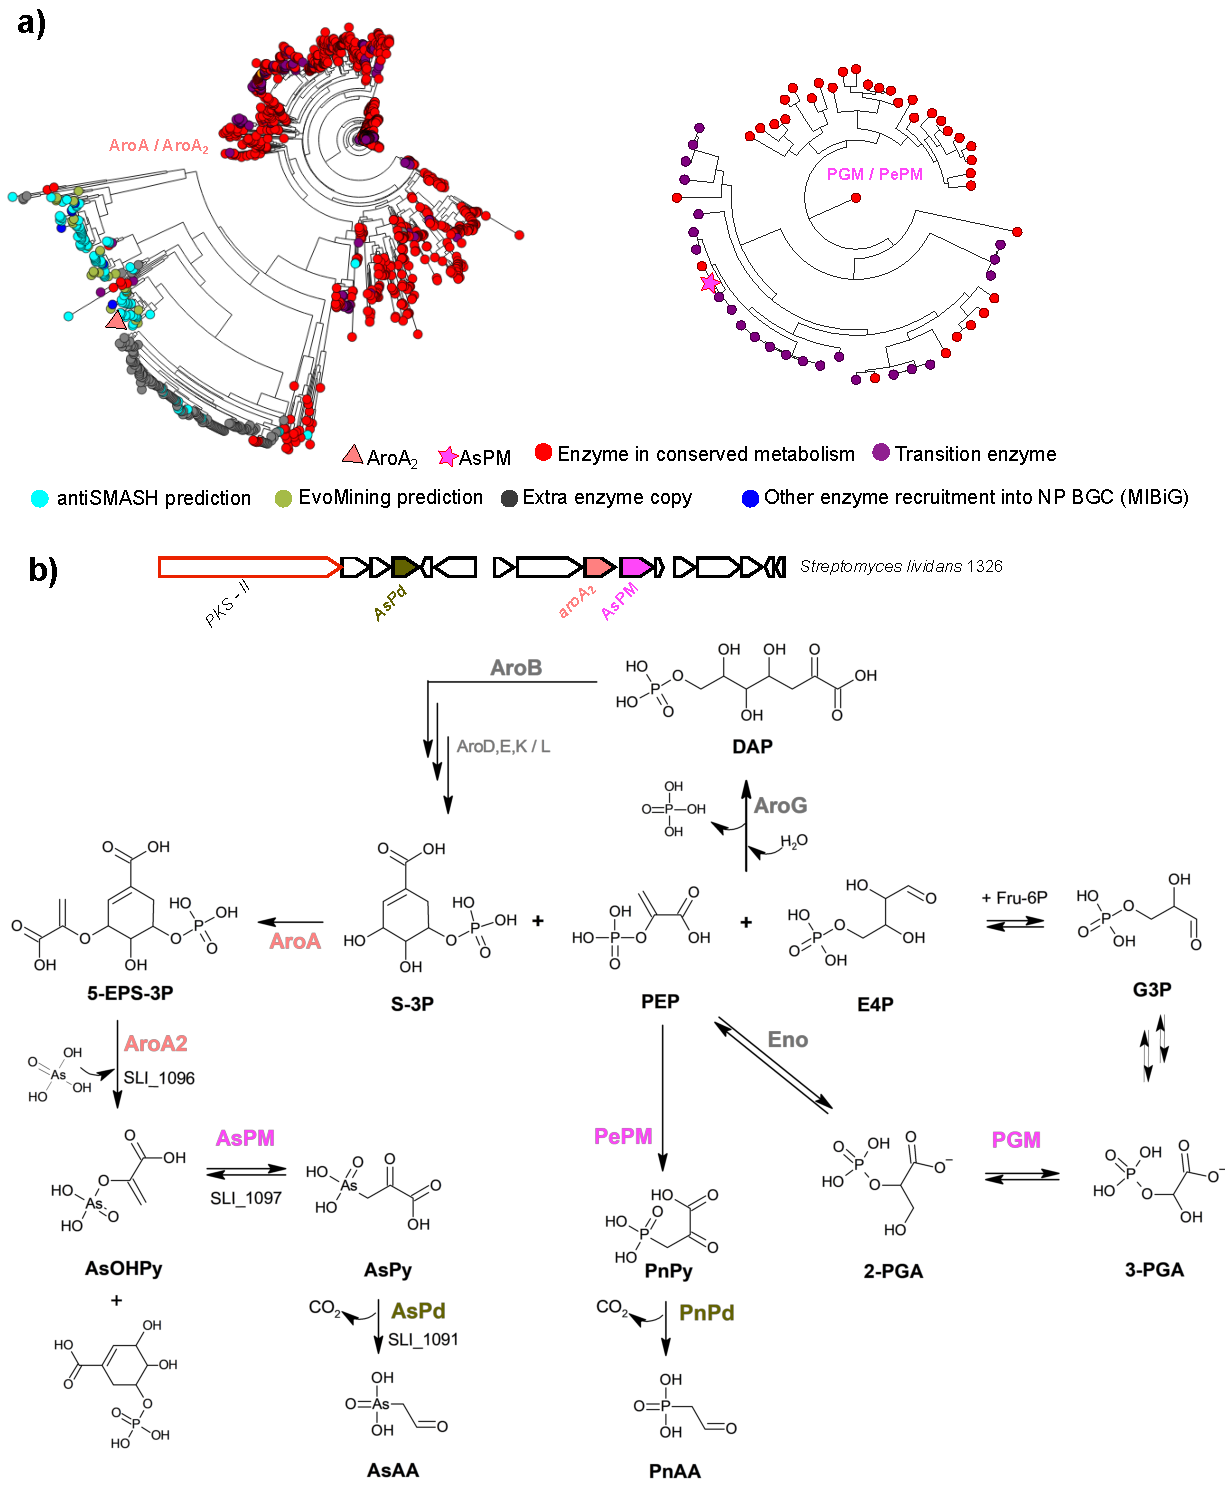
\includegraphics[angle = 0,scale = 0.6]{Arseno.pdf}
  \caption[El paradigma de EvoMining permitió localizar familias de enzimas de metabolismo central con copias extra que habían sido reclutadas para una nueva función en metabolismo especializado. Un ejemplo de ello es AroA, que cataliza una reacción similar pero sobre un sustrato diferente. La copia primaria cataliza una reacción sobre un metabolito con azufre y la secundaria sobre un metabolito con arsénico]{\normalsize{El paradigma de EvoMining permitió localizar familias de enzimas de metabolismo central con copias extra que habían sido reclutadas para una nueva función en metabolismo especializado. Un ejemplo de ello es AroA, que cataliza una reacción similar pero sobre un sustrato diferente. La copia primaria cataliza una reacción sobre un metabolito con azufre y la secundaria sobre un metabolito con arsénico}}
  \label{fig:Arseno}
  \end{figure}
  
  La búsqueda de productos naturales cuenta entre sus premisas que estos
  se producen en vecindades genomas llamadas clusters y que además
  clusters cercanos (ya sea en contenido génico o en la secuencia de sus
  componentes), exploran variaciones metabólicas, es decir sus enzimas
  catalizan reacciones sobre sustratos parecidos aunque no idénticos
  {[}\protect\hyperlink{ref-cruz-morales_phylogenomic_2016}{61}{]}. Los
  clusters de genes biosintéticos (BGC) de productos naturales que han
  sido caracterizados experimentalmente están depositados gracias el
  esfuerzo de toda la comunidad en la base de datos \emph{Minimal
  information about a biosynthetical gene cluster} MIBiG. Actualmente
  MIBiG cuenta con 1400 BGC.
  
  EvoMining ha demostrado incorporar efectivamente premisas evolutivas
  para localizar enzimas pertenecientes a estos BGC aún cuando pertenezcan
  a clases no conocidas. Análogamente otra herramienta de minería genómica
  ha utilizado con éxito la búsqueda de copias extra para encaminar su
  búsqueda específicamente a BGC de resistencia a antibióticos
  {[}\protect\hyperlink{ref-alanjary_antibiotic_2017}{84}{]}. Desarrollar
  EvoMining en combinación con algoritmos de búsqueda de cambios en la
  vecindad genómica la harán una plataforma ideal para abordar el problema
  de las familias, proporcionando una solución la dificultad de no tener
  conocimiento previo de un miembro promiscuo en la familia investigada.
  Respecto al problema de los miembros, se propone explorar variaciones en
  vecindad genómica, flujo génico y dinámica molecular, como candidatos a
  reflejar la variación en promiscuidad. Uno de los modelos modelo
  biológicos a explorar será el phylum Actinobacteria, un grupo de
  bacterias reconocido por su diversidad metabólica donde se ha probado la
  existencia de promiscuidad enzimática. Existen otros modelos
  interesantes como \(Pseudomonas\) y Cyanobacteria, linajes donde según
  MIBiG hay abundancia de BGC. En contraste Archaea no tiene más que un
  BGC reportado, esto puede deberse a un fenómeno biológico o bien a falta
  de exploración en dicho dominio. Aunque se ha avanzado tanto en el
  conocimiento de la promiscuidad en Archaea
  {[}\protect\hyperlink{ref-martinez-nunez_promiscuity_Archaea_2017}{85}{]}
  como en la detección de productos naturales, sin necesariamente
  caracterizar los genes biosintéticos
  {[}\protect\hyperlink{ref-charlesworth_untapped_natural_products_Archaea_2015}{86}{]}
  EvoMining podría ayudar a entender los patrones de expansión
  reclutamiento y sugerir familias con promiscuidad enzimática en este
  dominio.
  
  EvoMining es una plataforma bioinformática de análisis de expansión y
  reclutamiento de familias que puede ser utilizada para la identificación
  de enzimas que participan en clusters de síntesis de productos
  naturales. Si se combinara EvoMining con la premisa de que vecindades
  distintas son marcadoras de funciones químicas distintas, al encontrar
  una familia expandida con vecindades genomas diferentes se podría
  solventar la deficiencia de otros métodos bioinformáticos consistente en
  que para identificar familias promiscuas se debe conocer previamente un
  miembro promiscuo de la misma. Así pues al combinar EvoMining con
  herramientas de vecindad genómica tanto de comparación como de
  visualización estaremos mejorando su funcionalidad en la identificación
  de familias promiscuas.
  
  \section{La genómica comparativa como herramienta en la priorización de
  clusters
  promiscuos}\label{la-genomica-comparativa-como-herramienta-en-la-priorizacion-de-clusters-promiscuos}
  
  La promiscuidad nos interesa por su producción de variantes. Si bien en
  rutas centrales rescata la función, en metabolismo secundario crea
  nuevas variantes moleculares que permiten adaptación, de hecho
  pangenomas grandes correlacionan con aparición de nuevas funciones
  enzimáticas. Considero que el concepto de promiscuidad puede ser
  extendido a un nuevo nivel considerando a los clusters de genes
  biosintéticos como una nueva unidad. Así pues existiría la promiscuidad
  de una enzima, promiscuidad de una familia y promiscuidad de un cluster.
  
  \subsection{Expansión y contextos genómicos como herramienta de
  anotación
  funcional}\label{expansion-y-contextos-genomicos-como-herramienta-de-anotacion-funcional}
  
  Al evaluar la herramienta de análisis de promiscuidad PROMISE
  {[}\protect\hyperlink{ref-carbonell_molecular_2010}{28}{]} en un set de
  datos de la familia HisA/PriA
  {[}\protect\hyperlink{ref-noda-garcia_insights_2015}{50}{]} obtuve que
  en su mejor desempeño es (huella molecular de tamaño 6) clasifica
  correctamente casi todas las no promiscuas, (HisA) pero no sucede lo
  mismo con la familia PriA donde tiene éxito en 16 de 45 casos. Al
  aplicar el mismo tamaño de huella a 9 miembros promiscuos de la familia
  IlvC no consigue predecir correctamente ninguno de ellos reflejando tal
  vez que en su conjunto de entrenamiento no había miembros promiscuos
  \emph{ilvC}. Por lo menos para estas familias el conjunto de
  entrenamiento o los descriptores no son suficientes para la anotación de
  promiscuidad.
  
  La diversidad enzimática existente es el resultado de un proceso de
  expansión, mutación y selección que se ha desarrollado durante el
  transcurso de la historia evolutiva
  {[}\protect\hyperlink{ref-khersonsky_enzyme_2010}{5}{]}. Existe
  evidencia de que cierto grado de promiscuidad o divergencia funcional
  precede a la duplicación génica
  {[}\protect\hyperlink{ref-hughes_evolution_1994}{69}{]}. Por este motivo
  detectar expansiones ya sea duplicaciones o transferencias horizontales
  {[}\protect\hyperlink{ref-treangen_horizontal_2011}{88}{]}, puede ser un
  buen punto de partida para determinar divergencia funcional y
  promiscuidad. No todas las expansiones denotan cambio de función
  enzimática, algunas pueden ser meros accidentes, sin embargo dado que la
  función de una enzima suele estar relacionada con sus vecinos
  {[}\protect\hyperlink{ref-overbeek_use_1999}{89}{]}, una expansión en
  una vecindad genoma diferente de la tradicional sera un referente de
  adquisición de una nueva función y entonces un indicador de existencia
  previa de promiscuidad.
  
  Para sistematizar el estudio de contextos y vecindades genómicas se
  desarrollo Search Tool for the Retrieval of Interacting Genes/Proteins
  STRING {[}\protect\hyperlink{ref-snel_string_2000}{90}{]}, que cuenta
  con una anotación de orto logia jerárquica y consistente, realizada en
  2000 organismos en cuyo marco interacciones de proteínas con
  implicaciones funcionales son predichas tanto de novo por información
  genómica de co-ocurrencia como por minería de datos en artículos
  publicados. STRING es una base de datos, y como tal no permite agregar
  nuevos genomas para su análisis. Sus 2000 organismos incluyen especies
  tanto bacterianas como eucariotas. Al existir tanta diversidad, los
  genomas disponibles para un genero o clase específicos son escasos,
  p.~g. de los mas de 300 genomas disponibles de \emph{Streptomyces} solo
  24 están incluidos.
  
  Para resolver la baja cobertura de STRING hacia ciertos grupos
  taxonómicos se pueden desarrollar scripts de vecindad genómica
  utilizando RAST (Rapid Annotation using Subsystem Technology); un
  servicio interactivo de anotación automática de genomas de bacterias y
  arqueas {[}\protect\hyperlink{ref-aziz_rast_2008}{91}{]} donde la
  función de cada gen se asigna de acuerdo a conocimiento previo de
  subsecuencias de organismos cercanos filogenéticamente, cuando es
  posible se incluye en un subsistema metabólico. Estamos en una era de
  explosión de datos genómicos, próximamente se espera contar con millones
  de genomas bacterianos incluso provenientes de bacterias no cultivables,
  por ello los algoritmos deben ser constantemente optimizados a los
  nuevos volúmenes de datos
  {[}\protect\hyperlink{ref-medema_computational_2015}{53}{]}. Ante esta
  expectativa seria muy útil desarrollar algoritmos de análisis genómico
  que sean de código libre o al menos interactivos para que cada
  laboratorio pueda personalizarlos para sus propios genomas.
  
  Finalmente, no solo la vecindad genómica inmediata puede ser utilizada
  como distintivo en la búsqueda de promiscuidad, diferencias en el
  contexto genómico en genes relacionados con una enzima promiscua, sin
  importar su ubicación dentro del genoma también pueden ser relevantes
  para la perdida o ganancia de función química
  {[}\protect\hyperlink{ref-noda-garcia_evolution_2013}{31}{]},
  {[}\protect\hyperlink{ref-juarez-vazquez_evolution_2017}{47}{]}.
  
  \subsection{Contexto y vecindades
  genomicas}\label{contexto-y-vecindades-genomicas}
  
  En 2012 fueron analizados 102 genomas de 29 familias de Actinobacteria
  {[}\protect\hyperlink{ref-noda_tesis_2012}{75}{]}. sugiriendo que al
  menos en \emph{Corynebacteria} el contexto y la vecindad genómica
  incidían en la sub-funcionalización de PriA en subHisA
  {[}\protect\hyperlink{ref-noda-garcia_evolution_2013}{31}{]}. Respecto a
  IlvC, otra familia involucrada en la síntesis de aminoácidos fue
  estudiada y caracterizada bioquímicamente en 1 \(Corynebacterium\) y 8
  \(Streptomyces\)
  {[}\protect\hyperlink{ref-verdel-aranda_molecular_2015}{32}{]}. Para
  ampliar estos resultados, utilizando la anotación de RAST y una
  generalización de la definición de vecindad de STRING, se diseño un
  algoritmo para identificar vecindades similares así como uno de
  visualización de contexto, ambos disponibles como software libre en
  github \href{https://github.com/nselem/perlas}{nselem/perlas} .
  
  El algoritmo de clasificación de vecindades permite agruparlas en
  clusters y calificar estos clusters según su conservación dado un grupo
  de bacterias. La definición de vecindad y similitud de vecindad esta
  descrita posteriormente en los métodos. El algoritmo fue aplicado a la
  familia IlvC en 290 \emph{Streptomyces} resultando 9 clusters
  \href{http://148.247.230.43/nselem/CONTEXTS/REL_St275/ilvC/Contextos.php}{Datos}
  entre los mas poblados el primero cuenta con 279 elementos, otro con 9
  elemento y dos mas con 7 miembros (Fig 3), resultados experimentales son
  congruentes con que existe divergencia funcional entre miembros de
  clusters distintos
  {[}\protect\hyperlink{ref-verdel-aranda_molecular_2015}{32}{]}
  
  Natural products genomic
  era{[}\protect\hyperlink{ref-harvey_re-emergence_2015}{93}{]}
  
  \section{Estudio de una familia PriA}\label{estudio-de-una-familia-pria}
  
  \subsection{Caracterizacion in vivo}\label{caracterizacion-in-vivo}
  
  No todas las familias promiscuas provienen de expansiones, tal es el
  caso de PriA en Actinobacteria, donde no tiene expansiones y hasta el
  momento no se le conoce participación en rutas de metabolismo
  especializado. La promiscuidad de PriA parece debida al rescate de la
  función TrpF. Algunas enzimas PriA no han mostrado promiscuidad \emph{in
  vitro} pero si \emph{in vivo} ya que sobreviven en un medio sin
  triptofano, es decir \emph{in vivo} complementan la función TrpF.
  
  \subsection{Caracterizacion bioquimica in
  vitro.}\label{caracterizacion-bioquimica-in-vitro.}
  
  De la familia PriA y sus subfamilias se han caracterizado
  bioquímicamente miembros selectos de \emph{Actinomycetaceae},
  \emph{Bifidobacteriaceae}, \emph{Micrococcaceae},
  \emph{Acidimicrobiaceae}, \emph{Corynebacterium}, Mycobacteriaceae,
  Streptomycetaceae, Camera (provenientes de metagenoma), reconstrucciones
  ancestrales, 80 mutantes de \emph{Corynebacterium}, y 2 mutantes de
  Camera mediante cinéticas enzimáticas para calcular las constantes
  \(K_{cat}\),\(K_m\). El genero \(Streptomyces\), el que cuenta con mayor
  cantidad de genomas disponibles representa una oportunidad muy poco
  explotada de explorar la influencia del contexto y la vecindad genómicas
  en secuencias de PriA.
  
  \subsection{Modelado de dinamica
  molecular}\label{modelado-de-dinamica-molecular}
  
  La dinámica es un método que permite hacer simulaciones de partículas
  que sirve para obtener información de propiedades macroscópicas de un
  conjunto de átomos
  {[}\protect\hyperlink{ref-petrenko_molecular_2001}{94}{]}. Es útil en el
  marco de mi proyecto porque permite la exploración del espacio
  conformacional, y se ha visto que este esta relacionado con la actividad
  de la enzima {[}\protect\hyperlink{ref-sikosek_biophysics_2014}{96}{]},
  ademas dado un confórmero permite verificar su estabilidad. Resuelve la
  ecuación de movimiento de Newton con base a una configuración inicial,
  las fuerzas interatomicas como los enlaces covalentes, las fuerzas de
  Van der Waals y la carga de las
  partículas{[}\protect\hyperlink{ref-campbell_biophysical_2012}{54}{]}.
  Entonces para generar una simulación de dinámica molecular, debe
  contarse con una estructura como punto de partida, ya sea esta
  cristalográfica o modelada de novo o por homología. El laboratorio de
  bioinformática y biofísica computacional ha desarrollado un protocolo de
  generación de modelos homólogos estructurales y dinámicas moleculares
  (Carrillo-Tripp in prep); con este pipeline se han generado dos
  estructuras de Camera
  {[}\protect\hyperlink{ref-noda-garcia_insights_2015}{50}{]}, 30
  estructuras y dinámicas de miembros de Actinobacteriaceae y
  Bifidobacteriaceae
  {[}\protect\hyperlink{ref-juarez-vazquez_evolution_2017}{47}{]} y
  finalmente una estructura de subHisA de \emph{Corynebacterium
  diphteriae}. En el género \emph{Streptomyces}, interesante debido a su
  variación en contexto genómico y en mediciones \emph{in vitro} aun no se
  modelan dinámicas moleculares ni se habían realizado estructuras por
  homología previo a este trabajo.
  
  En conclusión la promiscuidad enzimática es un fenómeno complejo debido
  a múltiples causas. Existe una gran variedad de estudios con enfoques
  puntuales sobre aspectos estructurales, dinámicos y evolutivos sin
  embargo hasta ahora no se han reportado trabajos multidisciplinarios que
  involucren a todas las partes involucradas
  
  \clearpage  
  
  \chapter*{Objetivos}\label{objetivos}
  \addcontentsline{toc}{chapter}{Objetivos}
  
  \section{Objetivo General}\label{objetivo-general}
  
  Estudiar el fenomeno de promiscuidad tanto desarrollando estrategias
  para identificar familias promiscuas, miembros promiscuos en dichas
  familias o clusters biosintéticos promiscuos dentro de un grupo
  taxonómico, como comparando variaciones de promiscuidad \emph{in vitro}
  con variaciones en contexto genómico y en propiedades relacionadas a la
  estructura tridimensional en miembros de una familia.
  
  \section{Objetivos particulares}\label{objetivos-particulares}
  
  \begin{enumerate}
  \def\labelenumi{\arabic{enumi}.}
  \item
    Desarrollar Orthocore un método para entendercuáles son los genes más
    conservados en el \emph{core genome} en un linaje taxonómico y aplicar
    este conocimiento.
  \item
    Mejorar EvoMining como método de identificación de familias
    enzimáticas promiscuas aprovechando los cambios en vecindades
    genómicas como características informativas provenientes de datos
    filogenómicos.
  \item
    Desarrollar CORASON una herramienta Optimizar el entendimiento de la
    evolución de clusters biosintéticos y vecindades genómicas diversas,
    para poder organizarlas jerárquicamente tal y como se pueden organizar
    las secuencias de enzimas. Con este conocimiento proponer y verificar
    mediante BGC promiscuo y verificar la hipótesis
  \item
    Estudiar la relacion entre historias filogenómicas y procesos
    biofísicos con la promiscuidad \emph{in vitro}, a través de mediciones
    de ciertas características de la familia PriA.
  \end{enumerate}
  
  \clearpage  
  
  \chapter*{Estrategias}\label{estrategias}
  \addcontentsline{toc}{chapter}{Estrategias}
  
  \subsubsection{Obtener informacion genomica de diversos linajes
  genómicos.}\label{obtener-informacion-genomica-de-diversos-linajes-genomicos.}
  
  Colectar genomas de Actinobacteria, Cyanobacteria, \emph{Pseudomonas} y
  Archaea de NCBI y de colecciones privadas.
  
  \subsection{Anotar consistentemente las secuencias codificantes de estos
  genomas.}\label{anotar-consistentemente-las-secuencias-codificantes-de-estos-genomas.}
  
  Utilizar un anotador automatizado y desarrollar los scripts necesarios
  para automatizar la anotación de los genomas.
  
  \subsubsection{Establecer las relaciones filogenéticas de los genomas
  colectados.}\label{establecer-las-relaciones-filogeneticas-de-los-genomas-colectados.}
  
  Mediante el uso del \emph{core genome} construir un arbol filogenomico
  que permita establecer un marco sobre el cual hablar de cambio.
  
  \subsection{La promiscuidad en familias
  enzimaticas.}\label{la-promiscuidad-en-familias-enzimaticas.}
  
  Desarrollar Evomining hasta el punto de convertirla en una distribución
  funcional de código libre disponible para otros investigadores. Agregar
  características que faciliten la investigación como la visualización de
  la vecindad genomica de los miembros de una familia y otros metadatos
  como el número de copias por organismo.
  
  \paragraph{Identificar cambios en la vecindad genomica en familias
  selectas de enzimas de metabolismo
  central.}\label{identificar-cambios-en-la-vecindad-genomica-en-familias-selectas-de-enzimas-de-metabolismo-central.}
  
  Identificar familias de metabolismo central en los linajes genómicos
  seleccionados.
  
  Identificar mediante EvoMining las familias de metabolismo central con
  expansiones y reclutamientos que pueden presentar promiscuidad
  enzimática.
  
  Desarrollar las herramientas bioinformáticas necesarias para entender la
  conservación y evolución de BGCs u otras vecindades genomicas a las que
  pertenecen las expansiones de las familias centrales previamente
  seleccionadas.
  
  \subsubsection{Promiscuidad in vitro dentro de miembros de una familia
  promiscua de
  enzimas.}\label{promiscuidad-in-vitro-dentro-de-miembros-de-una-familia-promiscua-de-enzimas.}
  
  Dados los sustratos conocidos de PriA investigar las posibles
  correlaciones entre mediciones de constantes cataliticas, contexto
  genomico, vecindad genómica, estructura tridimensional y cambio en el
  número de copias en diversos linajes.
  
  \subsubsection{Sistematizar Evomining para convertirla una plataforma
  descargable y utilizable en cualquier set de datos bacterianos
  relacionados taxonomicamente proporcionados por el
  usuario.}\label{sistematizar-evomining-para-convertirla-una-plataforma-descargable-y-utilizable-en-cualquier-set-de-datos-bacterianos-relacionados-taxonomicamente-proporcionados-por-el-usuario.}
  
  -Ampliar el contenido de Evomining para poder analizar nuevas bases de
  datos genómicas, agregando por ejemplo los nuevos genomas colectados de
  Actinobacteria, así como los genomas de Cyanbacteria, \(Pseudomonas\) y
  Archaea.\\
  Sistematizar la base de datos de metabolismo central.
  
  -Desarrollar la visualizacion e integrar la clasificacion de vecindades
  genomicas como una herramienta adicional en la busqueda de promiscuidad.
  
  \subsubsection{Seleccionar miembros homologos de la familia de enzimas
  para modelado
  molecular.}\label{seleccionar-miembros-homologos-de-la-familia-de-enzimas-para-modelado-molecular.}
  
  Se escogieron 41 \emph{Streptomyces} repartidos en un arbol de rpoB de
  400 Streptomyces con genoma disponible. Esta selección incluye los seis
  \emph{Streptomyces} de los que se cuenta con cinética enzimatica de
  PriA, tres de ellos con estructura cristalográfica.
  
  \subsubsection{Medir cinéticas enzimaticas, contexto genómico y vecindad
  genómica}\label{medir-cineticas-enzimaticas-contexto-genomico-y-vecindad-genomica}
  
  Estudiar la existencia de distintas vecindades genomicas. Determinar la
  cinetica enzimatica de PriA respecto a sustratos atípicos sugeridos por
  los estudios estructurales. Obtener mediante una colaboración 37 modelos
  estructurales por homología y modelar docking molecular.
  
  \clearpage  
  
  \chapter*{Metodologia}\label{metodologia}
  \addcontentsline{toc}{chapter}{Metodologia}
  
  A continuacion describiré la metodologia para cada una de las
  estrategias expuestas previamente. Todos los scripts desarrollados
  fueron escritos en perl y estan disponibles en github
  \url{https://github.com/nselem/perlas} y empacados como un contenedor de
  docker.
  
  \subsection{La promiscuidad en familias
  enzimaticas.}\label{la-promiscuidad-en-familias-enzimaticas.-1}
  
  \subsubsection{Actinobacteria genomica}\label{actinobacteria-genomica}
  
  Para obtener información genómica del phylum Actinobacteria mediante la
  coleccion de genomas de NCBI se revisaron todas las familias de
  Actinobacteria de la base genoma de NCBI y se seleccionaron los genomas
  con mínimo 5 genes por contig. Se crearon scripts para utilizar la
  interfaz e-utils de NCBI y descargar estos genomas desde la terminal a
  partir de una lista de identificadores. El mismo procedimiento se aplico
  a Cyanobacteria, \emph{Pseudomonas} y Archaea.
  
  \subsubsection{Annotación}\label{annotacion}
  
  Para anotar consistentemente las secuencias codificantes de estos
  genomas se utilizó el anotador automatizado RAST y se desarrollaron los
  scripts necesarios para anotar los genomas desde la terminal, conectado
  asi NCBI y RAST. Se empacaron estos scripts en una distribución docker
  de myrast.
  
  \subsubsection{Filogenia de la base de datos
  genómica}\label{filogenia-de-la-base-de-datos-genomica}
  
  Establecer las relaciones filogeneticas de los genomas colectados
  mediante el uso del \emph{core genome} para construir un arbol
  filogenómico, y para encontrar genes marcadores de un linaje taxonómico.
  Para obtener el \emph{core genome} y en base a el reclasificar los
  genomas se diseño el algoritmo Orthocore que generaliza el concepto de
  Best Bidirectional Hits (blast all vs all).
  
  Orthocore. Se realiza un blast all vs all de genomas deseados. Para cada
  secuencia, centrado en cada genoma se realiza una lista (estrella) de
  sus mejores hits bidireccionales. Si las listas de todos los genomas
  coinciden es un BBH multiple y se agrega la lista al core genome. Una
  vez con el \emph{core genome} completo se puede reconstruir la
  filogenia. Este metodo fue exitoso en la deteccion de una familia
  marcadora de \emph{Clavibacter michiganensis}.
  
  \subsubsection{Organización y presentación de familias extendidas
  mediante el desarrollo una plataforma
  bioinformática.}\label{organizacion-y-presentacion-de-familias-extendidas-mediante-el-desarrollo-una-plataforma-bioinformatica.}
  
  Se desarrolló EvoMining como una plataforma interactiva de consulta, se
  complementó con programas de visualización de árboles filogenéticos y
  contextos genómicos.
  
  \subsubsection{Algoritmo de reconstrucción filogenética y
  visualización}\label{algoritmo-de-reconstruccion-filogenetica-y-visualizacion}
  
  Las secuencias de las familias enzimáticas expandidas fueron alineadas
  con muscle v3.2{[}\protect\hyperlink{ref-edgar_muscle_2004}{97}{]} y
  curadas con Gblocks
  v0.91b{[}\protect\hyperlink{ref-castresana_selection_2000}{98}{]}. Los
  parámetros de Gblocks fueron fijados en incluir 5 posiciones como el
  mínimo tamaño de un bloque y diez posiciones como el máximo de
  posiciones contiguas no conservadas. La selección de color de las hojas
  del árbol fue automatizada utilizando Newick Utilities una serie de
  programas llamados desde la terminal para manipular árboles en formato
  Newick{[}\protect\hyperlink{ref-junier_newick_2010}{99}{]}. La anotación
  funcional de RAST en su versión
  clásica{[}\protect\hyperlink{ref-aziz_rast_2008}{91}{]} fue agregada al
  SVG.
  
  \subsubsection{Algoritmo de
  visualización}\label{algoritmo-de-visualizacion}
  
  Para facilitar el análisis visual de una vecindad genómica y a la vez
  generar imagenes de alta calidad exportables para su uso en
  publicaciones, se desarrolló código cuya salida es el formato
  \emph{Scalable Vector Graphics} (SVG). Este formato es básicamente un
  archivo de texto XML que contiene instrucciones para que navegadores
  como Chrome o firefox realicen un dibujo. Al ser vectores, las imágenes
  generadas en SVG no pierden resolucion al ser escaladas y justamente por
  ser escalables permiten explorar con detalle grandes cantidades de datos
  organizados por ejemplo en árboles filogenéticos. Los scripts estraen
  para cada gen información necesaria como coordenadas, dirección, función
  química. La anotación de función proviene de la anotacion de RAST, la
  visualización de vecindades genomicas fue desarrollada \emph{de novo}.
  Los primeros análisis de EvoMining, antes de la existencia de esta
  plataforma fueron desarrollados en el lenguaje perl; este lenguaje
  cuenta con un modulo para facilitar la elaboracion de SVG (perlmaven/SVG
  2015) por lo que se decidió utilizarlo y continuar el desarrollo en Perl
  para no agregar nuevos requerimientos y facilitar su portabilidad.
  
  Se amplificara Evomining de los 200 genomas con que contaba su version
  inicial a los 880 colectados mudando la curacion manual de su base de
  datos de rutas centrales a la anotacion por subsistemas de RAST.
  Finalmente se presentara la variacion en vecindades genomicos como una
  herramienta adicional que ayude en la busqueda de promiscuidad en
  familias de enzimas pertenecientes al metabolismo central.
  
  \subsection{Identificar cambios en la vecindad genomica en familias
  selectas de enzimas de metabolismo
  central.}\label{identificar-cambios-en-la-vecindad-genomica-en-familias-selectas-de-enzimas-de-metabolismo-central.-1}
  
  \subsubsection{Dinamica molecular}\label{dinamica-molecular}
  
  Para generar dinamicas moleculares primer lugar se recolectaran las
  estructuras tridimensionales de miembros de PriA de Actinobacteria.
  Despues se procedera a modelar por homologia las estructuras
  tridimensionales faltantes utilizando el pipeline del laboratorio de
  bioinformatica y biofisica computacional. Este pipeline utiliza el
  software Rosetta para el modelado para las estructuras y GROMACS
  Groningen Machine for Chemical Simulation,
  {[}\protect\hyperlink{ref-van_der_spoel_gromacs_2005}{100}{]} para el
  modelado de la dinamica molecular. Esta parte del trabajo se realizara
  en colaboracion con el laboratorio de bioinformatica y biofisica
  computacional.
  
  \subsection{Consideraciones}\label{consideraciones}
  
  Falsos negativos respecto a promiscuidad estan muy extendidos en la
  literatura y en las bases de datos, en parte porque la mayoria de las
  funciones son asignadas por similitud de secuencia y dado un falso
  negativo el error se propaga en secuencias similares. Por otro lado es
  muy dificil demostrar un verdadero negativo a menos que se prueben todas
  las posibilidades de sustrato para la enzima. Sin embargo el espacio de
  sustratos puede acotarse gracias a tecnicas como el docking que esta
  intimamente relacionado con la dinamica molecular
  {[}\protect\hyperlink{ref-campbell_biophysical_2012}{54}{]}. Limitar el
  espacio de sustratos puede retroalimentarse con el estudio de la
  promiscuidad in vivo y viceversa.
  
  Con los metodos propuestos en este trabajo solo se podra detectar
  perdida o ganancia de promiscuidad entre enzimas de organismos respecto
  a otros miembros dentro un grupo taxonomico, no asi el estado de
  promiscuidad intrinseco a la enzima. Si dada una enzima no se detectan
  variaciones en contexto, vecindad genomica o flexibilidad dentro de un
  grupo taxonomico cercano, entonces no podemos decir en principio nada
  acerca de la promiscuidad de la variante, posiblemente es promiscua pero
  al mantenerse constante en todos los parametros descritos, con estos
  metodos no se puede sugerir promiscuidad. Es posible que al mirar en un
  grupo taxonomico mas amplio se detecte una neofuncionalizacion de la
  familia aunque tambien es posible que exista una variable z como la
  flexibilidad de sustrato
  {[}\protect\hyperlink{ref-nobeli_protein_2009}{23}{]} que no se este
  considerando y que explique o sea el mejor indicador para esta familia
  de promiscuidad enzimatica.
  
  Se debe considerar que si existe una correlacion vecindad
  genomica-promiscuidad, esta no indica causa efecto, mas bien, es
  plausible que la vecindad sea un amplificacion de diferencias en
  secuencia, a un numero igual de variaciones en secuencia la existencia
  de un cambio de vecindad indica un proceso mas largo y mas cambios, es
  una amplificacion de las marcas dejadas por transformaciones
  funcionales.
  
  Si bien no se resuelve el problema de anotar promiscuidad
  automaticamente, este trabajo pretende aprovechar que los contextos
  genomicos ayudan a la identificacion de familias promiscuas para mejorar
  una plataforma de productos naturales, pretende tambien una confirmacion
  de que los cambios en la dinamica molecular ayudan a identificar los
  miembros mas promiscuos hacia actividades recien adquiridas, asi como
  tambien ser pionero en la investigacion de promiscuidad in vivo.
  
  \chapter{Orthocore: una herramienta computacional para entender el
  pangenoma de un linaje
  genómico.}\label{orthocore-una-herramienta-computacional-para-entender-el-pangenoma-de-un-linaje-genomico.}
  
  La organización filogenética de un linaje genómico permite la
  observación de dinámicas de pérdida y ganancia de familias génicas en
  organismos cercanos. Si los organismos están desordenados
  taxonómicamente es difícil apreciar la dinámica de
  aparición-desaparición por genoma de ortólogos que son miembros de una
  familia génica. Así pues, ordenar los genomas de un linaje de acuerdo a
  su historia evolutiva facilita apreciar cambios en el número de copias
  de una familia. Esta consideración es relevante en el marco de esta
  tesis ya que cambios en la ocurrencia de promiscuidad pueden estar
  relacionados a copias extra de organismos
  cercanos{[}\protect\hyperlink{ref-verdel-aranda_molecular_2015}{32}{]}.
  Como se explicó previamente en la introducción, el pangenoma de un
  linaje taxonómico está dividido en el \emph{core}, \emph{shell} y
  \emph{dispensable} \emph{genome}. Orthocore es un algoritmo que se
  desarrolló para automatizar la obtención del \emph{core conservado} de
  un linaje genómico. Con este \emph{core} realiza una reconstrucción
  filogenética de los organismos del linaje \autoref{fig:Orthocore}. En
  esta sección se explica el funcionamiento de Orthocore así como casos en
  donde fue utilizado, específicamente en casos de estudio de los órdenes
  \emph{Actinomycetales}{[}\protect\hyperlink{ref-juarez-vazquez_evolution_2017}{47}{]},
  \emph{Micrococcales}{[}\protect\hyperlink{ref-rodriguez_tesis_2016}{102}{]}
  y
  \emph{Nostocales}{[}\protect\hyperlink{ref-gutierrez-garcia_cycad_2019}{103}{]}
  y en el género \emph{Salmonella}
  {[}\protect\hyperlink{ref-delgado-suarez_whole_2018}{104}{]}. Finalmente
  se describen otros métodos implementados para entender el pangenoma de
  un linaje genómico que han sido utilizados en aplicaciones relacionadas
  al patógeno del tomate \emph{Clavibacter
  michiganensis}{[}\protect\hyperlink{ref-rodriguez_tesis_2016}{102}{]}.
  
  \begin{figure}[h!tbp]
  \centering
  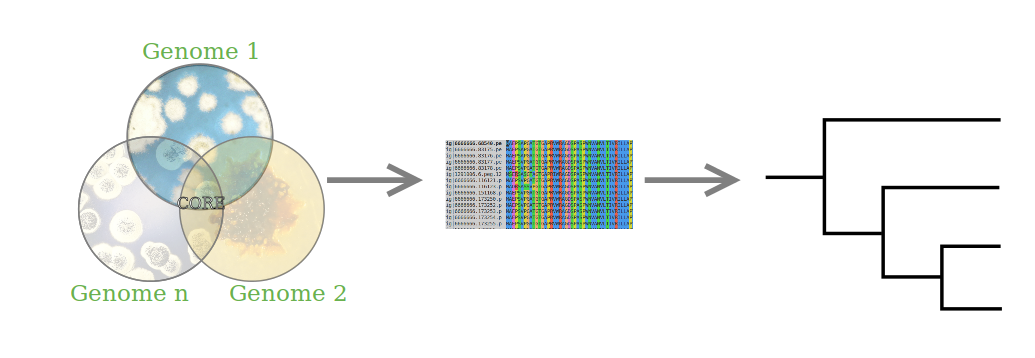
\includegraphics[angle = 0,scale = .44]{chapter1/coreWiki.png}
  \caption[Orthocore calcula el $core~genome$ de un linaje y construye con él una filogenia]{\footnotesize{Orthocore calcula las familias génicas comunes de un linaje taxonómico. Después de un proceso de filtrado, alineamiento y curación, Orthocore concatena las secuencias de estas familias y entrega una reconstrucción filogenética.}}
  \label{fig:Orthocore}
  \end{figure}
  
  \section{La distribución de la función metabólica de las familias del
  pangenoma depende de la variabilidad del linaje
  seleccionado.}\label{la-distribucion-de-la-funcion-metabolica-de-las-familias-del-pangenoma-depende-de-la-variabilidad-del-linaje-seleccionado.}
  
  El número de familias génicas presentes en el pangenoma, así como su
  distribución en el \emph{core}, \emph{shell} y \emph{dispensable genome}
  depende de la elección de los genomas y del linaje genómico. Para
  entender esto se puede pensar en un ejemplo extremo, consideremos una
  bacteria con 1000 familias de genes de la cual se secuencian diez
  genomas de la misma cepa. Estas secuencias deberían ser prácticamente
  idénticas y en ese caso el \emph{core genome} sería 1000 familias, el
  \emph{shell} y el \emph{dispensable genome} serían cero. En este caso,
  todo el metabolismo, tanto el central como el especializado estarían
  conservados dentro del \emph{core genome}, ya que el \emph{shell} y el
  \emph{dispensable genome} se encuentran vacíos. Sin embargo, si variamos
  el linaje taxonómico, y ahora estudiamos el pangenoma de 10 especies
  distintas del género \emph{Streptomyces} ahora el \emph{core genome}
  estará compuesto por aproximadamente un tercio de su tamaño. Dentro del
  \emph{core genome} es donde se encontrarán muchos de las familias
  dedicadas al metabolismo central o conservado (por ejemplo, familias de
  la glicólisis o síntesis de aminoácidos). En cambio muchas de las
  familias dedicadas al metabolismo especializado y pertenecientes a
  clústers biosintéticos de productos naturales (BGCs) estarán en el
  \emph{dispensable genome} pues \emph{Streptomyces} es productor de una
  gran variedad de metabolitos especializados y cada especie suele tener
  su producto característico. \autoref{fig:MetabolismoPangenoma}.
  
  \begin{figure}[h!tbp]
  \centering
  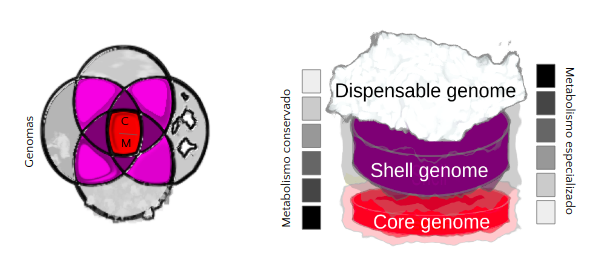
\includegraphics[angle = 0,scale = .75]{chapter1/Metabolismo-Pangenoma.png}
  \caption[El metabolismo en el Pangenoma]{\footnotesize{El pangenoma de un conjunto de genomas de un linaje puede ser clasificado en varios grupos. En este ejemplo, en el lado izquierdo de la figura se observa en gris el $genoma~dispensable$ compuesto por familias génicas presentes sólo en un genoma. En dos tonos de morado observamos el $shell genome$, familias que están presentes en la mayoría de los genomas del linaje, en este en caso dos o tres genomas. Finalmente en rojo se muestra el $core$, aquellas familias presentes en todos los genomas del linaje. El $core$ contiene tanto familias muy conservadas con una sola copia por genoma ( C ), como familias expandidas. Las familias marcadoras (M) pueden ser parte del $core$ conservado o de las familias expandidas. Del lado derecho se muestra una representación del pangenoma para cualquier número de genomas. Familias de metabolismo conservado tenderán a estar concentradas entre el $core$ y el $shell~genome$, mientras que el metabolismo especializado tendrá más representantes en el dispensable que en el $core genome$. Sin embargo tanto el tipo de metabolismo como el tamaño del $core$, $shell$ y $genoma~dispensable$ pueden variar según la diversidad de los organismos seleccionados. }}
  \label{fig:MetabolismoPangenoma}
  \end{figure}
  
  El \emph{core genome} de un linaje se puede usar para encontrar familias
  marcadoras \autoref{fig:CoreMarcadores} . Estos genes marcadores
  permiten realizar pruebas que diagnostiquen la presencia de organismos
  de ese linaje. A las familias que están presentes en el \emph{core
  genome} de un linaje A, pero que están completamente ausentes de un
  linaje B se les llama marcadoras. Por ejemplo genes conservados en la
  especie \emph{Streptomyces coelicolor} pero ausentes en
  \emph{Streptomyces rimosus} son genes marcadores de \emph{Streptomyces
  coelicolor} respecto de \emph{Streptomyces rimosus}. Estos mismos
  marcadores tal vez no sean marcadores respecto de \emph{Streptomyces
  lividans}, a pesar de la cercanía taxonómica entre estos organismos. La
  presencia de genes marcadores en el core depende de ambos linajes, y ya
  que es de interés científico y tecnológico encontrarlos en para
  identificar diferentes taxones es importante contar con algoritmos que
  permitan encontrarlos de forma automatizada.
  
  El número de familias en el pangenoma, ya sea en el \emph{core},
  \emph{shell} o \emph{dispensable genome} no sólo depende de la
  divergencia o proximidad taxonómica de los organismos del linaje
  seleccionado, también depende de lo variable que sea el contenido génico
  en los genomas del linaje. A esta característica se le conoce como
  apertura. Hay especies, por ejemplo algunos patógenos, cuyo pangenoma se
  encuentra sumamente cerrado en el sentido de que no importa cuántos
  genomas se agreguen, el número de familias parece converger y ser
  asintótico rápidamente a una cota superior. En cambio especies o géneros
  que viven en una gran diversidad de hábitats suelen tener un pangenoma
  abierto. Esto significa que cada vez que se agrega un nuevo genoma
  aparecen otras familias que no estaban en los genomas anteriores. En los
  linajes con pangenoma abierto el número de familias nuevas al agregar un
  genomas seguirá una tendencia creciente y no asintótica. Además de la
  apertura, existen otros intentos de cuantificar la diversidad génica de
  un linaje. Está por ejemplo la fluidez, definida como el promedio de
  familias únicas entre familias totales por pares de genomas. El
  pangenoma bacteriano total, es decir el total de familias génicas en el
  dominio Bacteria es considerado abierto.
  
  \begin{figure}[h!tbp]
  \centering
  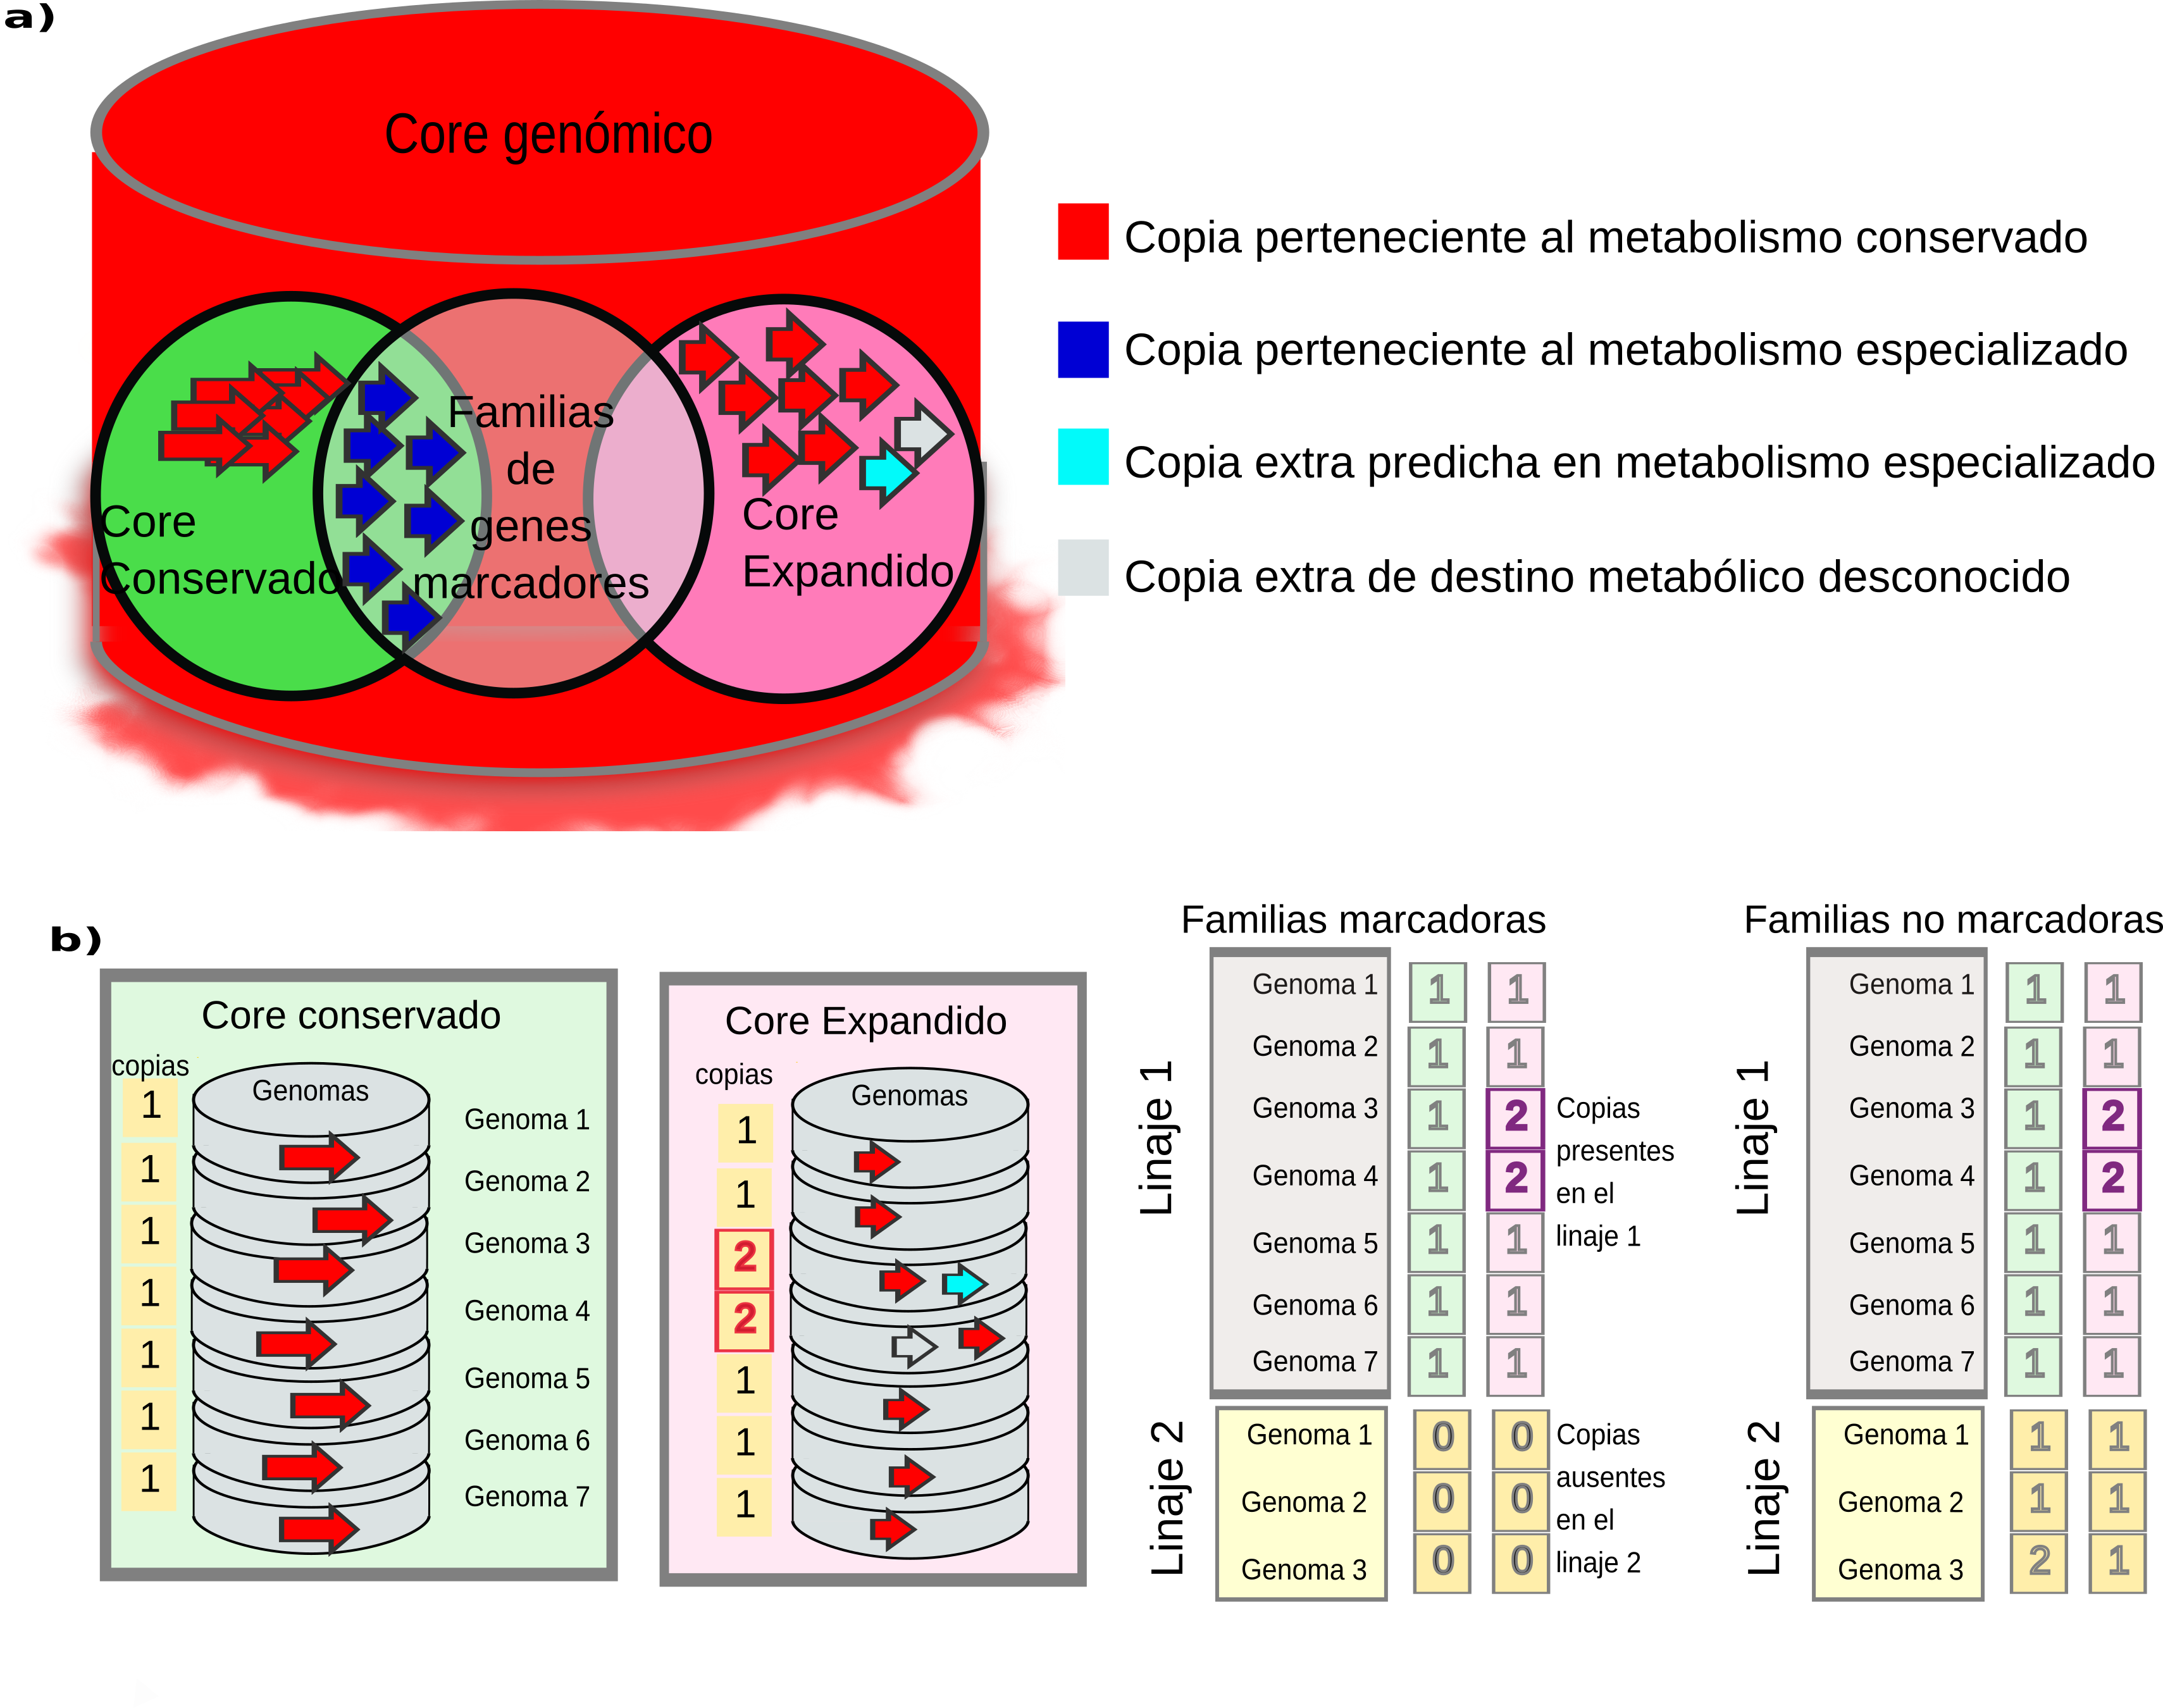
\includegraphics[angle = 0,scale = .8]{chapter1/CoreMarcadores.png}
  \caption[Core y genes Marcadores]{\footnotesize{El core genome puede contener familias con funciones en distintos grupos metabólicos así como diversidad en el número de copias. Arriba se muestra que en el core pueden coexistir familias tanto de copia única como con expansiones. Las familias con funciones en el metabolismo conservado suelen concentrarse en el $core~genome$ (rojas), pero también dependiendo de los organismos seleccionados pueden encontrarse ya sea familias enteras o algunas copias dedicadas al metabolismo especializado (azul). No de todas las copias se conocerá su función, algunas pueden tener un destino metabólico desconocido (gris) o bien ser predichas por algún algoritmo como parte del metabolismo especializado (cyan).  Abajo a la izquierda se comparan familias del $core~conservado$ con exactamente una copia por genoma contra familias del $core~expandido$. Ambas pertenecen al $core$, pero en el $core~expandido$ hay dos genomas que tienen una copia extra en esta familia, unoa cyan y una gris, que podría dificultar la elección de los verdaderos ortólogos. A la derecha se ejemplifican familias de genes marcadores, útiles para identificar un linaje genómico. Tanto familias del $core~conservado$ como del $core~expandido$ pueden ser familias marcadores, siempre que exista al menos una copia de cada familia en el linaje 1 y ninguna copia en el linaje 2. Las familias dejan de ser marcadoras cuando el linaje dos contiene al menos una copia en algún genoma.}}
  \label{fig:CoreMarcadores}
  \end{figure}
  
  Finalmente, la distribución de las funciones metabólicas encontrada en
  los subconjuntos del pangenoma ( \emph{core}, \emph{shell} o
  \emph{dispensable genome} está relacionada a la proximidad filogenética
  de los organismos seleccionados en el estudio. Entre más diversos sean
  los organismos menos familias dedicadas exclusivamente a metabolismo
  especializado abundarán en el \emph{core/shell genome}. La diversidad
  provocará que lo único que tengan los genomas de estos organismos en
  común sean funciones conservadas por una amplia variedad de especies
  bacterianas. Ahora bien, muchas familias de metabolismo especializado
  provienen de reclutamientos de copias extra de familias de metabolismo
  conservado. Así pues aunque decrezca el número de familias con
  exclusividad en metabolismo especializado en el \emph{core y shell
  genome}, estos subconjuntos del pangenoma aún pueden contener familias
  conservadas que tengan copias extra en proceso de reclutamiento para
  algún \emph{Cluster} biosintético de genes (BGC) de metabolismo
  especializado. Considerando las reflexiones anteriores, entre más
  diverso sea un linaje, más tenderá su \emph{core genome} a contener
  exclusivamente familias de metabolismo conservado mientras que su
  \emph{dispensable genome} estará formado mayormente por familias de
  enzimas del metabolismo especializado.
  
  \section{El core conservado permite la reconstrucción de filogenias
  complicadas}\label{el-core-conservado-permite-la-reconstruccion-de-filogenias-complicadas}
  
  Orthocore es el desarrollo bioinformático que realicé para calcular las
  familias génicas más conservadas del \emph{core genome}. Dos genes son
  homólogos si poseen un ancestro común, entre los principales grupos de
  homólogos están ortólogos y parálogos. Los ortólogos provienen de
  eventos de especiación de un ancestro común mientras que los parálogos
  evolucionan por eventos de duplicación. Orthocore obtiene un subconjunto
  del \emph{core genome}: el \emph{core conservado}, es decir, familias de
  ortólogos presentes en todos los genomas del grupo y que además son
  libres de parálogos de difícil identificación. El \emph{core conservado}
  facilita la organización en árboles filogenéticos de organismos de un
  linaje genómico.
  
  La comparación de la variación molecular entre ortólogos ha sido
  utilizada para establecer relaciones filogenéticas entre organismos.
  Esta técnica ha dado lugar a grandes descubrimientos. Por ejemplo
  comparar la secuencia de la subunidad 16S del gen RNA ribosomal (16S
  rRNA) condujo a Woese al descubrimiento del dominio Archaea en 1977
  {[}\protect\hyperlink{ref-woese_phylogenetic_1977}{105}{]}. Un árbol de
  especies suele hacerse con secuencias de familias que pertenecen al
  \emph{core genome} de un Dominio, por ejemplo las familias 16S rRNA o
  RpoB en los Dominios Bacteria y Archaea. Algunos autores realizan
  árboles multilocus para mejorar la resolución de árboles de especies
  realizados mediante la comparación de secuencias de 16S rRNA. Los genes
  seleccionados para los árboles multilocus deben estar en todos los
  organismos y no tener copias extra tan parecidas que puedan confundirse
  y entorpecer la reconstrucción filogenética, es decir, las familias
  seleccionadas deben ser parte del \emph{core conservado}. Orthocore
  automatiza la identificación de estas familias.
  
  Entre los factores importantes para establecer las relaciones
  filogenéticas que diferencian a las Archaeas de las Bacteria están los
  siguientes: 1) la presencia conservada de la subunidad de 16S en los dos
  dominios y 2) la suficiente divergencia entre estas secuencias en los
  organismos de dichos dominios. Ahora bien, establecer relaciones
  filogenéticas entre Archaea y Bacteria es en cierto sentido más sencillo
  que establecerlas entre organismos pertenecientes al mismo género o
  inclusive a la misma especie. En ocasiones, como en el caso del género
  \emph{Streptomyces}, la secuencia de 16S rRNA por sí sola no posee la
  suficiente variación para resolver la filogenia
  {[}\protect\hyperlink{ref-labeda_phylogenetic_2017}{106}{]}. En
  \emph{Streptomyces} la variación entre estas secuencias suele ser menor
  al 1\%. Para resolver el problema de escasa variación en secuencias de
  16S rRNA se pueden concatenar las secuencias de otros ortólogos, siempre
  que estos aparezcan en todos los organismos que se estén estudiando, es
  decir, siempre que sean parte del core genómico.
  
  \section{El algoritmo de Orthocore}\label{el-algoritmo-de-orthocore}
  
  Orthocore encuentra los genes del \emph{core} conservado en todos los
  genomas que se le proveen. Para poder ejecutarlo, el usuario tiene que
  proveer como entrada un conjunto de secuencias genómicas que ya debieron
  haber sido procesados por RAST, es decir ya deben tener anotaciones
  funcionales de los genes presentes en dichos genomas. El algoritmo de
  Orthocore encuentra los genes que están conservados como ortólogos en
  todas las secuencias y proporciona como salida una matriz con todos los
  genes y secuencias del \emph{core} es decir, todos los genes que
  resultaron mejores hits multidireccionales
  \autoref{fig:Best-n-directional}. Una vez que tiene todas las secuencias
  realiza una reconstrucción filogenética con las secuencias de
  aminoácidos y entrega la segunda salida, que es un árbol en formato
  árbol en formato Newick. Con estas salidas se puede visualizar la
  filogenia de los organismos en cuestión, identificar cuáles genes son
  parte del \emph{core}. Una parte central de este algoritmo consiste en
  determinar cuáles genes realmente son ortólogos confiables para
  reconstruir la filogenia.
  
  \subsection{\texorpdfstring{Los mejores hits multidireccionales definen
  los genes del \emph{core}
  conservado}{Los mejores hits multidireccionales definen los genes del core conservado}}\label{los-mejores-hits-multidireccionales-definen-los-genes-del-core-conservado}
  
  Los ortólogos suelen identificarse por similitud de secuencia, pero si
  se realiza la identificación manualmente también se suelen capturar
  parálogos que pueden confundir la elucidación de eventos de especiación.
  Orthocore automatizó la búsqueda de ortólogos y el filtrado de parálogos
  en genomas procariontes mediante la generalización de la definición del
  mejor hit bidireccional (BBH por sus siglas en inglés)
  \autoref{fig:Best-n-directional}. Dos secuencias son BBH si cada una es
  el mejor hit de un algoritmo de distancia (BLAST usualmente) en el
  genoma de origen de la otra. Una primera generalización para obtener el
  set de ortólogos de una familia del core es definir un genoma de
  referencia y tomar los BBH respecto a ese genoma. En la práctica, esta
  definición da como resultado distintos resultados según el genoma de
  referencia, haciendo que algunos parálogos no sean filtrados.
  
  Para solventar esta dificultad se definió en Orthocore el concepto de
  mejores hits multidireccionales. Un conjunto de genes son mejores hits
  multidireccionales si todos entre sí son BBH por pares y cada uno de los
  miembros de ese conjunto de genes pertenece a cada una de las secuencias
  genómicas. Es decir si cada gen fuera un punto y ser mejor hit se
  expresara como una conexión con dirección todos los puntos estarían
  conectados por una flecha de ida y otra de regreso. Con este método se
  eliminó la dependencia de un genoma de referencia. Esta restricción
  también ocasiona que en grupos muy grandes por ejemplo más de 100
  genomas de distintas especies, o muy diversos de distintos dominios, o
  muy fragmentados como con contigs de en promedio 3 Mbp, el \emph{core
  conservado} puede quedar vacío.
  
  \begin{figure}[h!tbp]
  \centering
  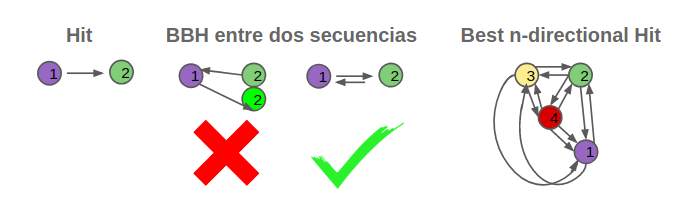
\includegraphics[angle = 0,scale = .55]{chapter1/Best-n-directional.png}
  \caption[Los mejores hits n-direccionales generalizan a los $Bidirectional~Best~Hits$]{\footnotesize{Orthocore utiliza los mejores hits n-direccionales para obtener grupos de ortólogos. Un hit es el mejor resultado de una secuencia en otro genoma. Un Bidireccional Best Hit es el mejor hit bidireccional. La secuencia 2 es el mejor hit de la secuencia 1 en el genoma 2 y recíprocamente, la secuencia 1 es el mejor hit de la secuencia 2 en el genoma 1. La existencia de una copia extra muy parecida a la secuencia 2 puede romper el BBH. Un mejor hit n-direccional debe ser BBH todos contra todos garantizando que estas secuencias están muy conservadas entre sí.}}
  \label{fig:Best-n-directional}
  \end{figure}
  
  \subsection{Ejecución de Orthocore}\label{ejecucion-de-orthocore}
  
  Orthocore es un tubería escrita en Perl que incorpora los hits
  multidireccionales permitiendo obtener y usar el \emph{core conservado}
  para realizar una reconstrucción filogenética mediante los siguientes
  pasos:
  
  -Obtiene el \emph{core conservado}: los mejores hits multidireccionales
  (blastp).\\
  -Alinea cada familia del \emph{core conservado} (MUSCLE).\\
  -Cura automáticamente cada familia del \emph{core conservado}
  (Gblocks).\\
  -Concatena las familias del \emph{core conservado} formando una
  alineamiento multilocus de aminoácidos.\\
  -Provee una reconstrucción filogenética que se genera a partir del
  alineamiento (FastTree). -Provee los genes del \emph{core conservado} y
  su anotación funcional según RAST.
  
  Existen otros algoritmos como
  OrthoMCL{[}\protect\hyperlink{ref-li_orthomcl_2003}{62}{]}, y
  \href{https://github.com/grovesdixon/using_FastOrtho}{fastOrtho}{[}\protect\hyperlink{ref-wattam_patric_2014}{107}{]}
  que dividen pangenomas en clusters de familias de genes,
  \href{http://eead-csic-compbio.github.io/get_homologues/manual/}{get\_homologues}
  {[}\protect\hyperlink{ref-contreras-moreira_get_homologues_2013}{108}{]}
  y metaphor que obtienen el \emph{core} y filtran buscando verdaderas
  relaciones de homología, y finalmente
  BPGA{[}\protect\hyperlink{ref-chaudhari_bpga-_2016}{109}{]} que hace
  reconstrucciones filogenéticas tanto según el \emph{core} como según el
  pangenoma. Sin embargo Orthocore resolvió en su momento la necesidad
  específica de proporcionar un alineamiento concatenada de genes del
  \emph{core conservado} lista para utilizarse en un árbol multilocus.
  Adicionalmente, como Orthocore fue diseñado para trabajar con la
  anotación de la plataforma RAST, también se obtiene la anotación
  funcional tanto de familias del \emph{core} como del complemento.
  
  Orthocore incorpora todas las dependencias en un contenedor de docker
  disponible en \url{https://github.com/nselem/orthocore}. Además en este
  contenedor está un script que permite bajar genomas de NCBI masivamente
  y posteriormente anotarlos en RAST desde la terminal. Los protocolos de
  uso se encuentran al final de este capítulo.
  
  \section{\texorpdfstring{Aplicaciones de Orthocore, identificación del
  \emph{core conservado} y de familias de genes
  marcadores.}{Aplicaciones de Orthocore, identificación del core conservado y de familias de genes marcadores.}}\label{aplicaciones-de-orthocore-identificacion-del-core-conservado-y-de-familias-de-genes-marcadores.}
  
  Cuatro aplicaciones de Orthocore serán presentadas en las siguientes
  secciones de este capítulo. En la primera aplicación el \emph{core
  conservado} en \emph{Actinomycetales} permitió organizar
  filogenéticamente a este orden. Esta organización facilitó el
  entendimiento en cambios de promiscuidad de la familia enzimática PriA
  mediante la distinción de patrones de pérdida y ganancia de genes en las
  rutas de síntesis de histidina y triptófano. En la segunda aplicación
  cepas de \emph{Salmonella} fueron ordenadas filogenéticamente. La
  tercera aplicación permitió realizar una reconstrucción filogenética del
  orden \emph{Nostocales} del phylum \emph{Cyanobacteria} y comparar así
  patrones de presencia y ausencia de clusters de genes biosintéticos.
  Finalmente, en organismos del microbioma del tomate orthocore de utilizó
  para identificar genes marcadores que permitieran distinguir cepas de
  \emph{Clavibacter Michiganensis} de otras especies de
  \emph{Micrococcales}.
  
  \subsection{\texorpdfstring{Orthocore de \emph{Actinomycetales} para
  mejorar el árbol de
  especies}{Orthocore de Actinomycetales para mejorar el árbol de especies}}\label{orthocore-de-actinomycetales-para-mejorar-el-arbol-de-especies}
  
  A pesar de que se sabía que miembros de la familia PriA habían sufrido
  cambios de promiscuidad y de especificidad entre la función HisA de la
  vía de síntesis de histidina y la función TrpF de la biosíntesis de
  triptofano {[}\protect\hyperlink{ref-noda-garcia_evolution_2013}{31}{]},
  se desconocía cómo había ido cambiando la función de esta familia de
  genes durante los procesos de especiación en \emph{Actinomycetales}.
  Para eso se necesitaba entender filogenéticamente al orden
  \emph{Actinomycetales}, el camino que seguimos fue hacer una filogenia
  con las secuencias de su \emph{core conservado}. Orthocore fue diseñado
  para resolver este problema. Con el resultado de Orthocore se realizó un
  árbol de especies donde se observaron patrones de pérdida y ganancia de
  genes en la vecindad genómica del gen que codifica para PriA. Se
  encontró que hay clados de \emph{Actinomyces} donde los genes
  correspondientes a la síntesis de histidina no estaban en la vecindad
  genómica de PriA, y mediante la realización de cinéticas enzimáticas se
  comprobó que la actividad de catalizar la reacción correspondiente a
  HisA estaba perdida en estos organismos. A estas enzimas se les llamó
  subTrpF ya que sólo poseían la capacidad de catalizar la reacción
  correspondiente a la familia TrpF. Del mismo modo existían clados que
  perdieron los genes de síntesis de triptófano en la vecindad de PriA y
  estas enzimas se subfuncionalizaron a la familia subHisA. De estos datos
  se observa que en estos organismos la especiación coincidió con el
  cambio de promiscuidad en la familia PriA, acorde a la pérdida y
  ganancia de genes vecinos. Este caso es una muestra promiscuidad puede
  co-ocurrir con variaciones en el contexto genómico, pudiendo estos
  cambios ser una marca para sugerir cambio funcional en una familia. De
  esta forma, se pudo concluir que los perfiles de promiscuidad de PriA en
  el orden \emph{Actinomycetales} se relacionan con la especiación
  {[}\protect\hyperlink{ref-juarez-vazquez_evolution_2017}{47}{]}.
  
  \subsection{\texorpdfstring{Uso de Orthocore para entender la evolución
  de la patogénesis de \emph{Salmonella} en
  México.}{Uso de Orthocore para entender la evolución de la patogénesis de Salmonella en México.}}\label{uso-de-orthocore-para-entender-la-evolucion-de-la-patogenesis-de-salmonella-en-mexico.}
  
  Los genomas conocidos de \emph{Salmonella} en México están tan
  conservados en sus genes marcadores tradicionales que se dificultaba
  hacer una filogenia. Esta situación es común en cepas de la misma
  especie. En este caso era importante relacionar las especiaciones de
  cepas aparentemente no patogénicas y la evolución de las islas de
  patogenicidad que se sabía estaban presentes en la mayoría de los
  aislados.\\
  Por ello, como primer paso se desarrolló una distribución de myRAST en
  un contenedor de Docker que pudiera usarse en cualquier servidor. Esta
  tubería prepara los datos para Orthocore al realizar la anotación
  automática de genomas ensamblados en RAST. El
  \href{https://github.com/nselem/myrast}{protocolo de myRAST} está
  disponible en github y además puede encontrarse en los apéndices de esta
  tesis. Después, con los genomas ya anotados, Orthocore fue usado para
  reconstruir la filogenia de esos aislados de \emph{Salmonella}. Además
  se buscó cómo fue la evolución de las islas de patogenicidad de esas
  cepas mediante un análisis de CORASON
  {[}\protect\hyperlink{ref-navarro-munoz_computational_2018}{110}{]}, en
  el que visualizamos las islas de patogenicidad organizadas
  filogenéticamente. En este caso se observó una alta conservación de
  toxinas tifoidales en islas de patogenicidad de \emph{Salmonella}. Éstas
  fueron identificadas en 76\% de las cepas analizadas. Este análisis se
  publicó como parte de un trabajo donde además se mostró que las islas de
  patogenicidad no pueden ser marcadoras de la enfermedad ya que se
  encontró ganado sin síntomas de la enfermedad pero que sí contenía
  bacterias con estas islas
  {[}\protect\hyperlink{ref-delgado-suarez_whole_2018}{104}{]}.
  
  \subsection{\texorpdfstring{Las \emph{Nostoc} provenientes del
  metagenoma de cícadas están en el mismo grupo
  filogenético}{Las Nostoc provenientes del metagenoma de cícadas están en el mismo grupo filogenético}}\label{las-nostoc-provenientes-del-metagenoma-de-cicadas-estan-en-el-mismo-grupo-filogenetico}
  
  Cyanobacteria es un phylum de bacterias que se han adaptado a diversos
  ambientes. Aunque muchas de ellas son marinas algunas Cyanobacterias
  viven como simbiontes de plantas. En particular las cícadas han
  desarrollado un tipo especial de raíz donde se sabe que vive como
  simbionte el género \emph{Nostoc}. La presencia de \emph{Nostoc} en la
  raíz coraloide de las cícadas es fácilmente distinguible por la
  formación de un anillo verde conocido como anillo cyanobacterial. En la
  \autoref{fig:ArbolNostoc} se muestra la filogenia de 76 Cyanobacterias
  de 7 órdenes distintos construida con 198 proteínas del \emph{core
  conservado} obtenidas por Orthocore. En esta reconstrucción se puede
  observar que los \emph{Nostoc} asociados a plantas tienden a agruparse
  en la filogenia
  {[}\protect\hyperlink{ref-gutierrez-garcia_cycad_2019}{103}{]} lo que
  sugiere que entre las cianobacterias de nuestro set de datos pudiera ser
  que las 3 \emph{Nostoc} provenientes de raíz coraloide provengan de un
  evento de colonización. Queda por mostrar si esta filogenia corresponde
  a la de las cícadas simbiontes, lo que sugeriría una estrecha
  coevolución entre ambos organismos.
  
  \begin{figure}[h!tbp]
  \centering
  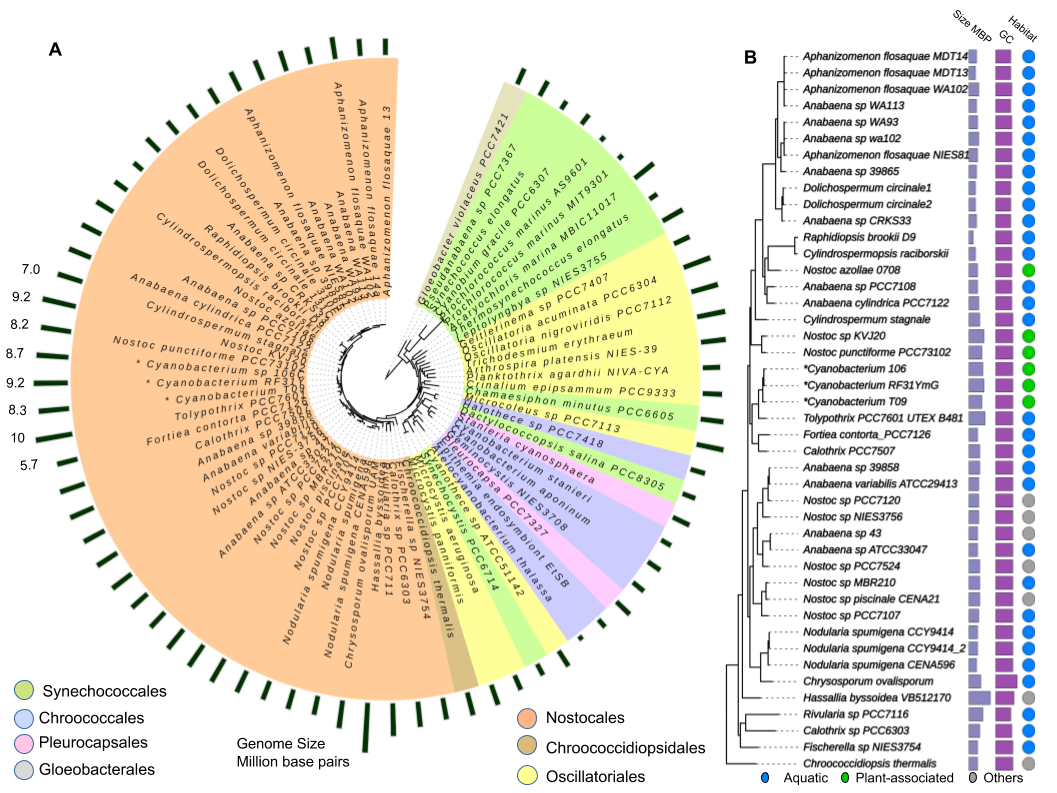
\includegraphics[angle = 0,scale = .45]{chapter1/Nostoc.png}
  \caption[Arbol filogenético de $Nostoc$ construido utilizando  la selección de genes del $core~conservado$]{\footnotesize{Reconstrucción de 76 taxa provenientes de 7 órdenes de Cyanobacteria. La matriz final incluyó 45,475 aminoácidos curados de 198 familias de proteínas pertenecientes al $core~conservado$. A la derecha se muestra un zoom sobre el orden $Nostocales$. En este orden se incluyen algunas bacterias simbiontes de cícadas. Metadatos como el tamaño de genoma, contenido de GC y hábitat de origen muestran una posible tendencia de incremento de tamaño en los genomas provenientes del microbioma de plantas.}}
  \label{fig:ArbolNostoc}
  \end{figure}
  
  \subsection{\texorpdfstring{Identificación de genes marcadores de la
  bacteria del `cáncer del tomate' \emph{Clavibacter
  michiganensis}}{Identificación de genes marcadores de la bacteria del cáncer del tomate Clavibacter michiganensis}}\label{identificacion-de-genes-marcadores-de-la-bacteria-del-cancer-del-tomate-clavibacter-michiganensis}
  
  Los \emph{Micrococcales} es un orden de Actinobacteria que contiene a
  \emph{Clavibacter}, \emph{Micrococcus} y \emph{Microbacterium}, entre
  otros microorganismos. El género \emph{Clavibacter} comprende especies
  que pueden causar enfermedades en diversas plantas. En particular la
  especie \emph{Clavibacter michiganensis} es una bacteria causante de la
  enfermedad del cáncer del tomate. \emph{Clavibacter michiganensis} ha
  sido frecuentemente aislada en compañía de otros \emph{Micrococcales}
  morfológicamente parecidos. La distinción entre microorganismos debida a
  la comparación de la secuencia de 16S rRNA no era suficiente para
  distinguir entre \emph{Micrococales} del microbioma del tomate, por lo
  que una prueba de diagnóstico se hacía necesaria. Se habían utilizado
  como marcadores genes como \emph{tomA}, \emph{ppaC} y \emph{celA} entre
  otros, sin embargo estas elecciones en ocasiones resultaban en falsos
  positivos según árboles de especies de 16S rRNA, por lo que nuevos
  marcadores eran necesarios.
  
  \begin{figure}[h!tbp]
  \centering
  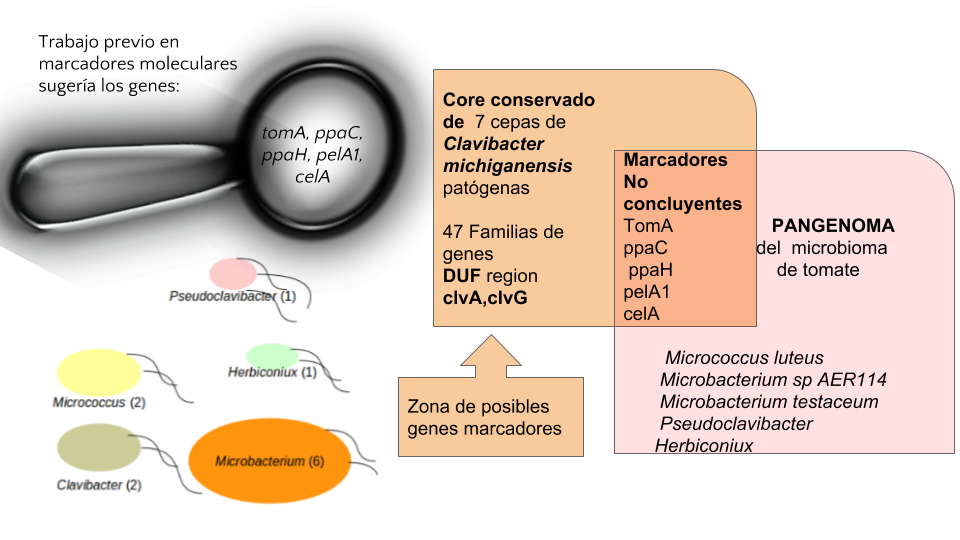
\includegraphics[angle = 0,scale = .5]{chapter1/Marcadores-Clavibacter.png}
  \caption[Los genes del cluster biosintético clv son marcadores de $Clavibacter$]{\footnotesize{Los marcadores moleculares previos a este trabajo no permitían diferenciar correctamente a $Clavibacter~michiganensis$ respecto al microbioma del tomate en invernaderos mexicanos. Arriba a la izquierda se muestran los antiguos marcadores $tomA, ppaC, ppaH, pelA1, celA$. Abajo organismos pertenecientes al microbioma del tomate. Orthocore obtuvo el core conservado de siete cepas de $Cmm$ patógenas, y este core se utilizó para definir nuevos marcadores. Aunque $tomA$ pertenecía al core conservado de $Cmm$, estaba también incluido en el pangenoma del microbioma del tomate. Después de calcular la intersección core conservado de $Cmm$ y pangenoma del microbioma se obtuvieron entre las familias marcadoras genes $clv$ parte del cluster biosintético de clavidicina (michiganina).}}
  \label{fig:Marcadores}
  \end{figure}
  
  Al analizar en Orthocore genomas de \emph{Microbacterium} y
  \emph{Micrococcus} aislados de tomate se encontró que \emph{tomA} y los
  otros marcadores propuestos previamente no eran exclusivos de
  \emph{Clavibacter michiganensis} ( \emph{Cmm} ). Al utilizar Orthocore
  en siete genomas de \emph{Cmm} encontramos que varios genes del cluster
  biosintético de michiganina (BGC0000528 en MIBiG) codificado por los
  genes \emph{clvAFGLKM} pertenecían al core conservado, pero que al
  agregar los genomas no \emph{Cmm} del resto del microbioma del tomate
  los genes \emph{clv} se pierden. El descubrimiento de que \emph{clv}
  pertenecía al core de \emph{Cmm} se realizó con secuencias de genomas
  muy fragmentados, en la\autoref{fig:Marcadores} se muestran las cepas
  originales que fueron analizadas.
  
  \begin{figure}[h!tbp]
  \centering
  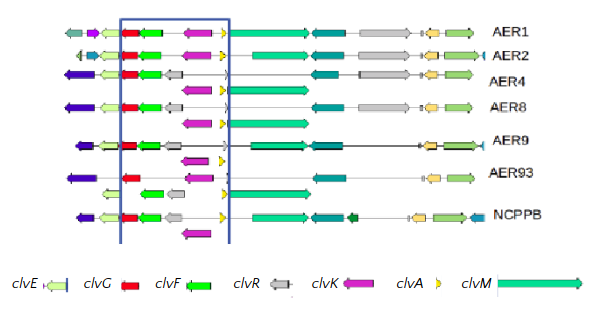
\includegraphics[angle = 0,scale = .6]{chapter1/clv.png}
  \caption[ El Cluster $clv$ es un marcador de la especie $Clavibacter~michiganesis$ en el orden $Micrococcales$.]{\footnotesize{El Cluster $clv$ es un marcador de la especie $Clavibacter~michiganesis$ en el orden $Micrococcales$. Los genes $clvEGAM$ que son una proteína de membrana, un transportador y dos proteína de síntesis del BGC $clv$ están muy conservados en la especie $Clavibacter~michiganensis$. $clvFRK$, es decir un transportador y el sistema de dos componentes están presentes en otros $Micrococcales$ pero con baja identidad de secuencia y nunca enel contexto del BGC de clavidicina}}
  \label{fig:clv-Marcadores}
  \end{figure}
  
  Esta observación se corroboró con más genomas,
  \autoref{fig:clv-Marcadores} en este caso se muestran como ejemplo 10
  genomas de bacterias del microbioma del tomate, entre ellas siete
  \emph{Clavibacter}, seis de tomates de invernadero y uno
  \emph{Clavibacter} proveniente de tomate silvestre y \emph{Clavibacter}
  RA1B. Con Orthocore vemos que el tamaño del core decrece al ir agregando
  genomas de \emph{Clavibacter} y decrece aún más rápido al agregar los
  genomas de \emph{Micrococcus} y \emph{Microbacterium} La reconstrucción
  filogenética de este microbioma, ubica a \emph{Clavibacter} RA1B cerca
  de los otros \emph{Cmm} pero no en un clado junto con ellos. Una
  búsqueda por blast revela que los genes marcadores de \emph{Cmm}:
  \emph{clvF}, \emph{clvR} son también marcadores de \emph{Clavibacter}
  RA1B pero no así \emph{clvA} y \emph{clvG} que solamente están presentes
  en el core de \emph{Cmm}. Sin embargo \emph{clvF} y \emph{clvR} no están
  en el contexto del cluster de michiganina en RA1B y su similitud de
  secuencia es menor que la que se observa entre los otros \emph{Cmm}.
  
  De hecho al considerar más genomas dentro del microbioma del tomate, la
  familia \emph{clvF} no solo no está en el core conservado de
  \emph{Microbacterium} y \emph{Micrococcus}, sino que no está presente en
  ningún otro genoma distinto a \emph{Clavibacter}. Con distintos niveles
  de conservación de secuencia los genes \emph{clv} son un buen marcador
  para distinguir \emph{Cmm} de otras especies, por esta razón estos genes
  aún se encuentran en uso como genes marcadores de \emph{Cmm}.
  Previamente se reportó que las familias \emph{clvA, clvF} y \emph{clvG}
  son exclusivas de \emph{Cmm}, de acuerdo a evidencia experimental
  {[}\protect\hyperlink{ref-yasuhara-bell_genes_2014}{111}{]} pero sin
  análisis genómicos que confirmaran que esos genes no estaban presentes
  en otras especies sin ser expresados. Este descubrimiento ha permitido
  bajar los costos de identificación de \emph{Clavibacter}, ya que ahora
  en lugar de enviar a secuenciar el genoma es suficiente identificar por
  PCR \emph{clvF} en conjunto con otros marcadores.\\
  Con Orthocore además de obtener los genes marcadores podemos obtener
  también la matriz del core conservado para realizar la reconstrucción
  filogenética de especies cercanas de \emph{Clavibacter}
  \autoref{fig:Clavibacter-EvoMining} . Ya que los productores querían
  conocer de dónde provienen las bacterias que infectan al tomate con el
  fin de evitarlas, se determinó la organización taxonómica de cepas de
  \emph{Cmm} y de otras bacterias del microbioma de tomate. Para esto se
  han secuenciado y mantenido como datos privados unos doscientos genomas
  provenientes del microbioma del tomate y se han analizado con Orthocore
  para obtener matrices multilocus que pueden diferenciar entre cepas de
  \emph{Clavibacter} de la misma o de diferente especie.
  
  \begin{figure}[h!tbp]
  \centering
  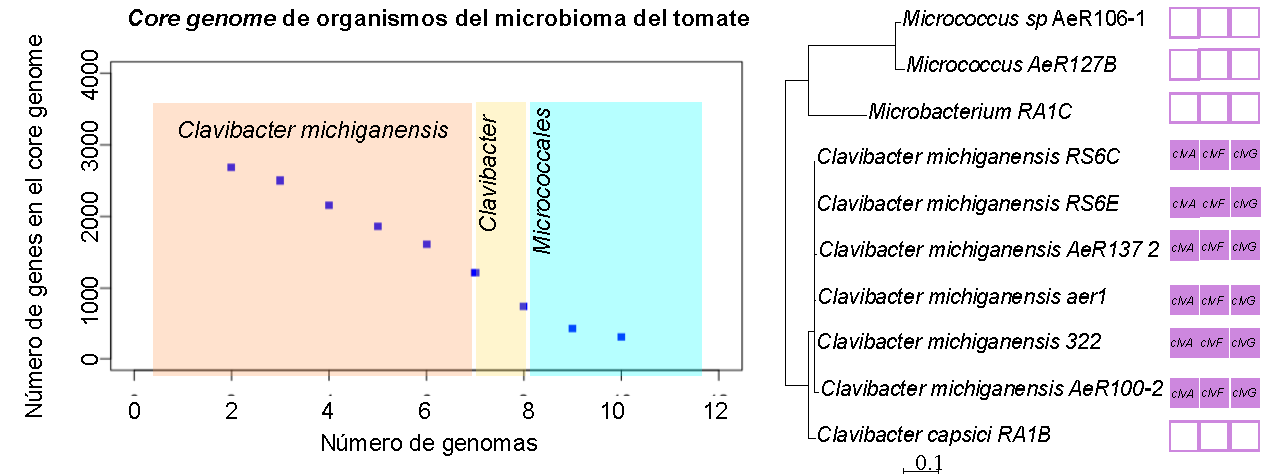
\includegraphics[angle = 0,scale = .7]{chapter1/CoreGenomeMicrobioma.pdf}
  \caption[El $core~genome$ de $Micrococcales$ ayuda a identificar genes marcadores ]{\footnotesize{El $core~genome$ de $Micrococcales$ ayuda a identificar genes marcadores. El $core~genome$ de siete organismos del microbioma del tomate muestra  de }}
  \label{fig:Clavibacter-EvoMining}
  \end{figure}
  
  Debido al intercambio génico por transferencia horizontal en las
  bacterias, es posible que los genes marcadores actuales alguna vez
  aparezcan en otros organismos. También las bacterias pierden
  continuamente genes, por lo que es posible que algún gen marcador de
  \emph{Cmm} se pierda en una cierta cepa . Esto hace que la definición de
  estar presentes en el core del grupo de interés y ausentes totalmente de
  cada uno de los genomas de otro linaje ya no funcione completamente. Sin
  embargo, en estas dos situaciones presentadas, ganancia de genes
  marcadores de organismos externos al linaje original o pérdida de genes
  marcadores en algunas cepas, se sigue cumpliendo que los ex genes
  marcadores, estarán presentes en la mayoría de los organismos del linaje
  de interés y ausentes de la mayoría de los organismos del linaje
  externo. Por ello, se pensó que está definición de genes marcadores se
  podía generalizar clasificando a grupos de genes ortólogos acorde a sus
  porcentajes de ocurrencia. Esta idea se desarrolló en la herramienta
  clavisual, explicada en la siguiente sección.
  
  \subsubsection{Clavisual: Identificación de genes marcadores a un cierto
  porcentaje de grupos
  seleccionados}\label{clavisual-identificacion-de-genes-marcadores-a-un-cierto-porcentaje-de-grupos-seleccionados}
  
  La idea de que Orthocore puede ser usado para obtener los genes
  marcadores de un grupo taxonómico frente a otro fue generalizada en el
  software Clavisual. Ya se ha explicado previamente que el core puede
  salir vacío por diversas razones, entre ellas baja calidad de los
  genomas, o que éstos provengan de organismos muy divergentes, verdaderas
  razones biológicas como dinámica génica o un core no convergente. Así
  pues, es posible que si sólo se utiliza el core no se obtengan
  marcadores. Pero el core puede relajarse de varias maneras una de ellas
  es el Pseudocore, donde en lugar de multidireccional hits se toman BBH a
  un genoma de referencia. Otra forma es establecer un porcentaje de
  presencia /ausencia de interés. El pseudocore consiste en utilizar
  información previa específica del core de un linaje para obtener los
  genes de y la metodología está depositada en github integrada en el
  repositorio
  \href{https://github.com/nselem/clavigenomics}{clavigenomics}. El blast
  fue optimizado cambiando hacer un blast todos contra todos por archivos
  genómicos individuales genomai\_vs\_genomaj.blast que luego son
  concatenados según se necesiten.
  
  Los porcentajes de genomas son diferentes porque al no bastar los
  mejores hits bidireccionales conservados, todo el pangenoma es decir
  todos los genes contenidos en los genomas del grupo de interés necesitan
  ser clasificados por familias, para de ahí obtener las familias que
  tienen presencia en un porcentaje \%p y ausencia en un porcentaje a\%
  del grupo externo. Estos perfiles fueron desarrollados para Clavisual
  \autoref{fig:Clavisual} utilizando FasthOrtho para clasificar las
  familias y de ahí obtener los grupos. Con ellos se consiguieron
  marcadores para \emph{Kurtobacterium}.
  
  Finalmente Clavisual despliega un árbol realizado con el Pseudocore
  respecto a un conjunto de genes de \emph{Cmm} NCPP previamente
  seleccionados. En este árbol clavisual permite la visualización de
  metadatos, como año, género de la bacteria, estado de salud de la planta
  e invernadero donde fue aislada.
  
  \begin{figure}[h!tbp]
  \centering
  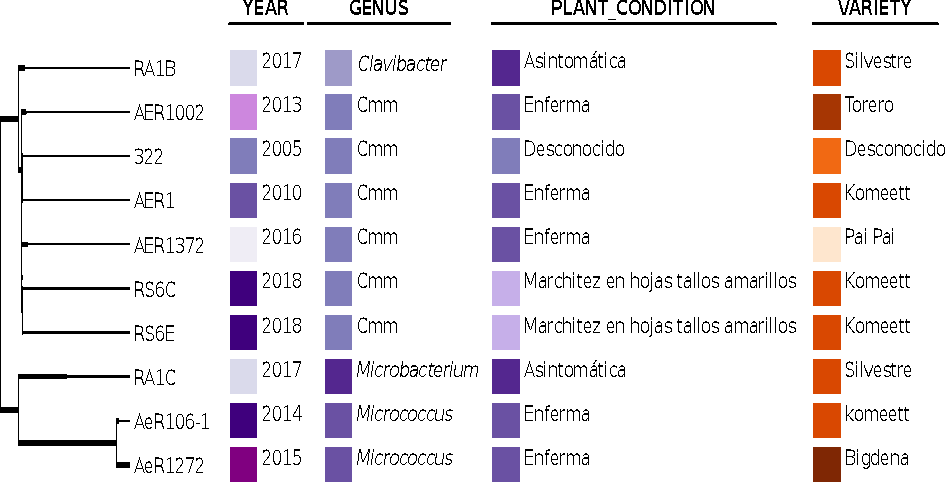
\includegraphics[angle = 0,scale = .7]{chapter1/Clavisual.pdf}
  \caption[Clavisual organiza cepas de $Clavibacter$ con sus metadatos. ]{\footnotesize{Clavisual organiza filogenéticamente cepas de $Clavibacter$ y generaliza orthocore. Clavisual no se restringe a la búsqueda del core conservado, permite la identificación de familias conservadas sólo en un cierto porcentaje. Además puede filtrar estas familias permitiendo sólo las que estén ausentes en una proporcion mínima de un grupo de genomas de interés. Además orthocore optimiza el funcionamiento de Clavisual ya que fue utilizado para proveer un conjunto de familias génicas conservadas en el género $Clavibacter$. Estas familias son buscadas cada vez que ingresa un genoma nuevo y con ellas se contruye un árbol filogenético. Los metadatos disponibles son desplegados al lado de la cepa correspondiente del árbol.}}
  \label{fig:Clavisual}
  \end{figure}
  
  \subsubsection{\texorpdfstring{El pangenoma de \emph{Clavibacter
  Michiganensis} es
  abierto}{El pangenoma de Clavibacter Michiganensis es abierto}}\label{el-pangenoma-de-clavibacter-michiganensis-es-abierto}
  
  Después de desarrollar métodos de identificación de genes marcadores y
  generalizarlo a obtener grupos con patrones de presencia/ausencia
  definidos por el usuario, quedaba por responder la pregunta cómo es el
  pangenoma de \emph{Cmm}. Algunos autores consideran que el pangenoma de
  patógenos es reducido porque sus genomas suelen sufrir proceso de
  reducción de tamaño debido a la pérdida de genes. Como \emph{Cmm} es un
  patógeno de planta quedaba por investigar cómo es su pangenoma. ¿Es
  posible saturar el contenido génico de \emph{Cmm} con sólo secuenciar
  más genomas?. Aunque actualmente existen ya herramientas web para el
  análisis de pangenoma, en su momento se utilizó el software
  \emph{Bacterial PanGenome Analysis Tool} que se corre desde la terminal.
  Para facilitar su instalación se desarrolló un contenedor Docker (ver
  abajo, descripciones técnicas). Como ejemplo de su funcionamiento, se
  analizó el pangenoma de los mismos diez genomas del tomate utilizados en
  la visualización de clavisual \autoref{fig:bpga-pangenoma} . Tomando
  otros siete genomas del género \emph{Clavibacter}, utilizando OrthoVenn
  tenemos la misma observación, el número de familias de genes agregadas
  al adicionar genomas, es después de siete genomas casi tan grande como
  su core \autoref{fig:Venn-Chart}.
  
  \begin{figure}[h!tbp]
  \centering
  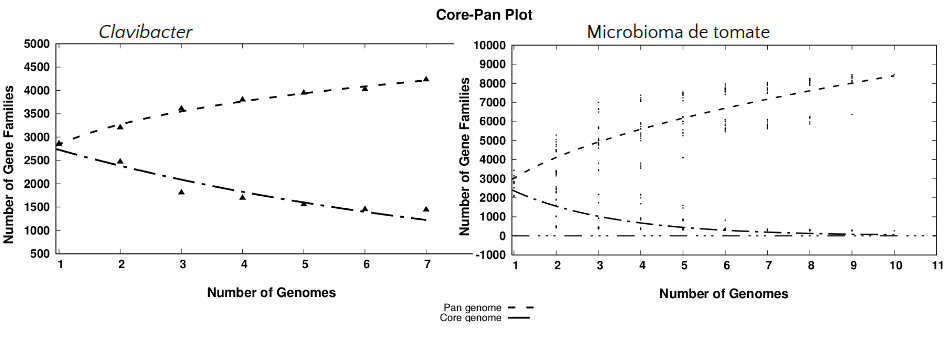
\includegraphics[angle = 0,scale = .5]{chapter1/bpga-pangenoma.png}
  \caption[El pangenoma de $Clavibacter$ es abierto según el análisis de BPGA.]{\footnotesize{El pangenoma de $Clavibacter$ es abierto según el análisis de BPGA. En este ejemplo el pangenoma de Clavibacter se mantiene creciente mientras que el core no alcanza el cero. En contraste, al ampliar el rango taxonómico el $core~genome$ sí se acerca a cero según BPGA}}
  \label{fig:bpga-pangenoma}
  \end{figure}
  
  \begin{figure}[h!tbp]
  \centering
  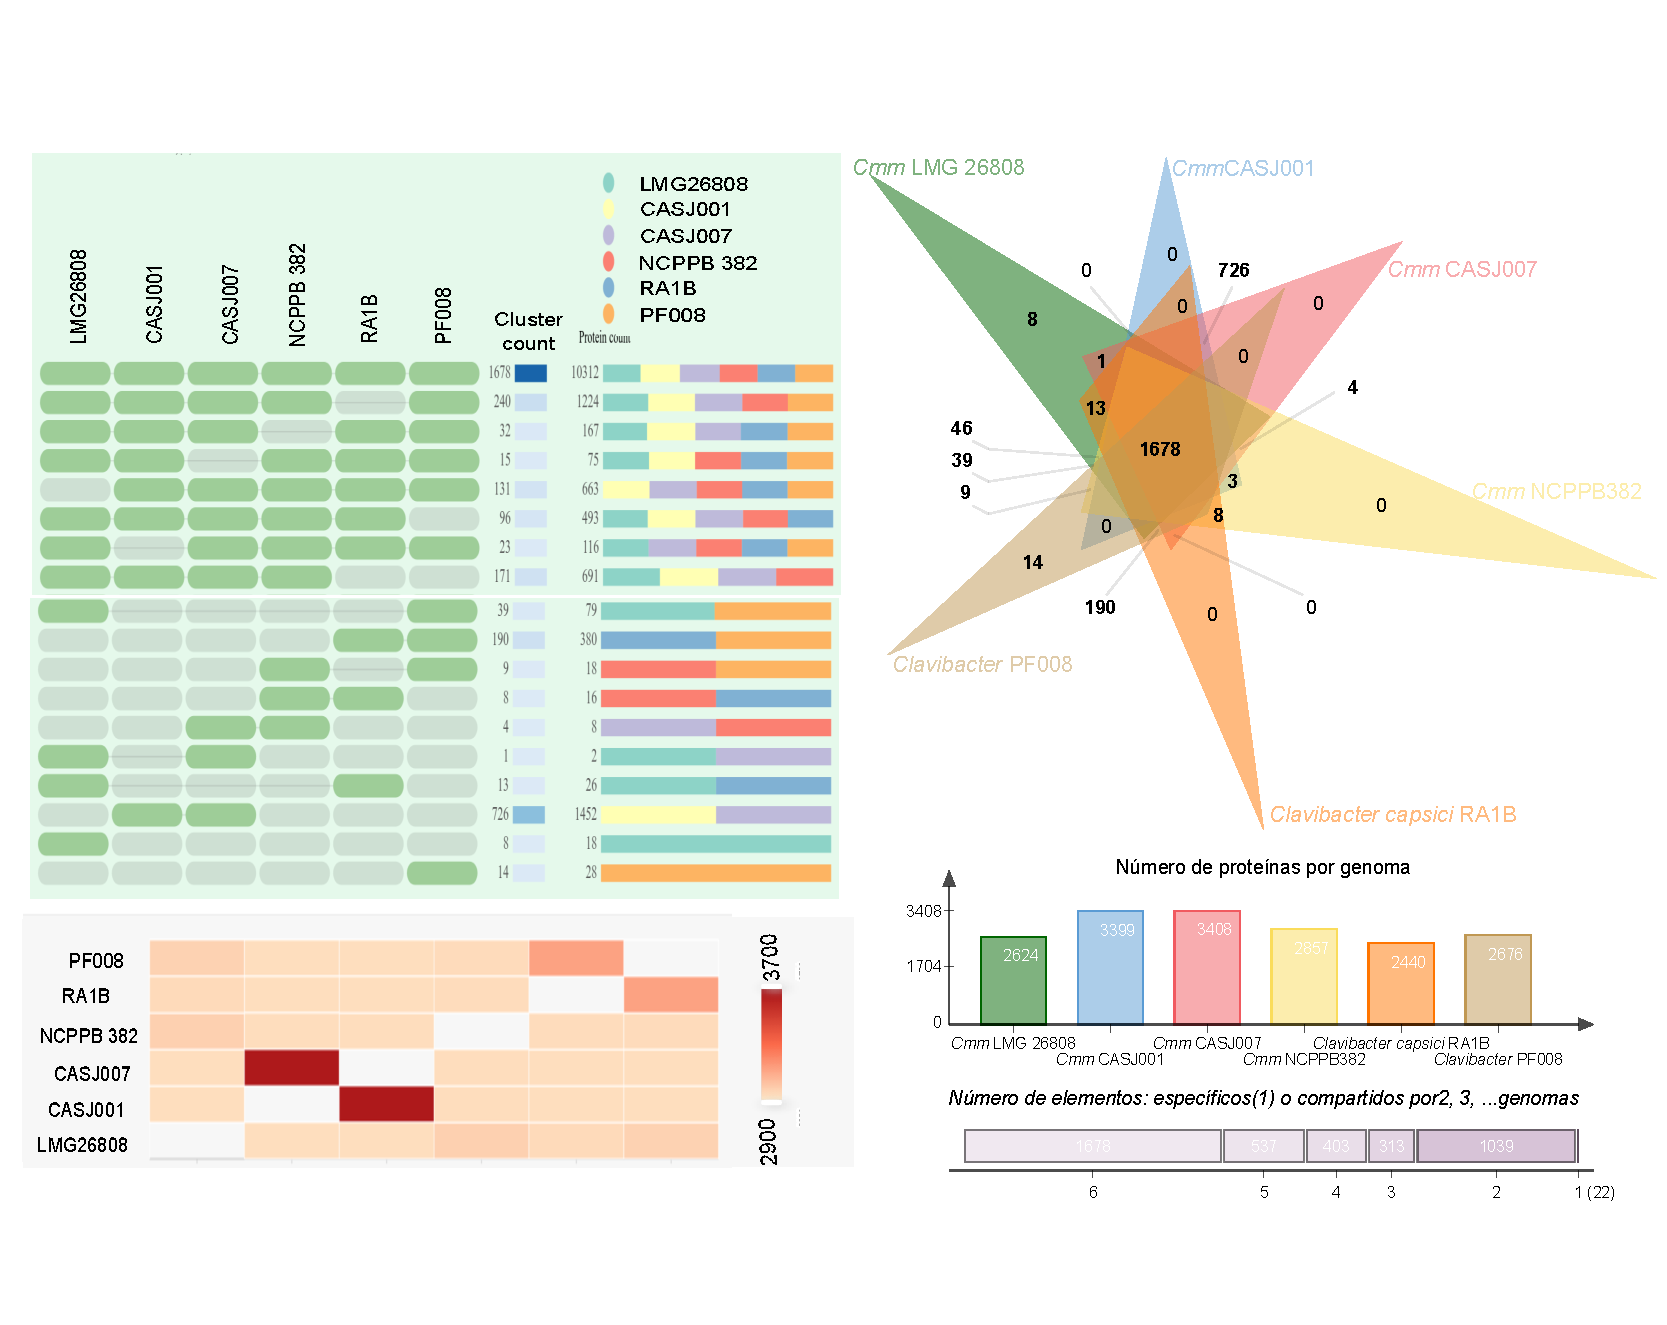
\includegraphics[angle = 0,scale = .6]{chapter1/Venn_chart.pdf}
  \caption[Diagrama de Venn del pangenoma de genomas selectos del género $Clavibacter$ ]{\footnotesize{Diagrama de Venn del pangenoma de genomas selectos del género $Clavibacter$. Venn-Chart permite visualizar la distribucion de las familias génicas mediante un diagrama de Venn siempre que sean pocos genomas. En la parte superior izquierda se muestra el número de familias compartidas entre distintos grupos de genomas. Por ejemplo existen 1678 familias génicas compartidas entre los seis genomas. Entre los grupos de cinco genomas, el más abundante es el que no contiene a RA1B con 243 familias, así pues RA1B es de los genomas más divergentes de este grupo.}}
  \label{fig:Venn-Chart}
  \end{figure}
  
  \section{Relación entre genes marcadores, Orthocore y la promiscuidad
  enzimática.}\label{relacion-entre-genes-marcadores-orthocore-y-la-promiscuidad-enzimatica.}
  
  Orthocore es pues una herramienta para detectar el \emph{core
  conservado}, es decir los genes del \emph{core genome} que o bien no
  tienen copias extra o éstas son tan diferentes de la copia primaria que
  no pueden ser confundidas con ella. En este capítulo aprendimos que los
  genes marcadores son parte del \emph{core conservado} de un grupo
  taxonómico, pero no necesariamente se dedican a lo que se entiende como
  metabolismo central en procariontes. Es decir el \emph{core conservado}
  no sólo está compuesto por rutas centrales como la síntesis de
  aminoácidos o la glicólisis. Como ejemplo de ello se mostraron familias
  pertenecientes al cluster de clavidicina \emph{clvABCDEF} que pertenecen
  al \emph{core conservado} de la especie \emph{Clavibacter michiganesis}
  pero que salen del core cuando se considera todo el linaje de
  \emph{Microccocales}, i.e.~no son parte del metabolismo central de ese
  orden. Estas consideraciones nos explican que no hay una relación uno a
  uno entre metabolismo central y genes del core. Según el linaje que se
  considere existen genes del core que no son esenciales, y existen
  también genes de metabolismo conservado en Bacteria que no están en el
  core de un linaje, como por ejemplo TrpF en Actinobacteria.
  
  Así pues en este capítulo aprendimos que con Orthocore podemos detectar
  los genes del \emph{core genome} que no tienen copias extra. En
  oposición, en el siguiente capítulo veremos qué pasa con los otros genes
  del core, los que sí tienen copias extra. Estas familias de genes como
  se mencionó en la introducción son interesantes porque pueden presentar
  promiscuidad enzimática debido a la retención de la función ancestral.
  Sin embargo, las familias expandidas no necesariamente tienen que
  provenir del core. El siguiente capítulo veremos que el \emph{shell
  genome} también puede presentar expansiones y que varias de ellas han
  sido reclutadas al metabolismo especializado. Esta búsqueda y
  clasificación de familias que han sido expandidas mediante copias extra
  fue sistematizada en el desarrollo de la herramienta EvoMining que es de
  lo que trata el siguiente capítulo.
  
  \chapter{EvoMining como herramienta para identificar el origen y el
  destino metabólico de familias
  enzimáticas}\label{evomining-como-herramienta-para-identificar-el-origen-y-el-destino-metabolico-de-familias-enzimaticas}
  
  \section{Introducción}\label{introduccion-1}
  
  \subsection{Las copias extra de familias enzimáticas que son reclutadas
  para una nueva función están relacionadas con la
  promiscuidad.}\label{las-copias-extra-de-familias-enzimaticas-que-son-reclutadas-para-una-nueva-funcion-estan-relacionadas-con-la-promiscuidad.}
  
  La promiscuidad enzimática puede buscarse en familias envueltas en
  procesos de divergencia funcional
  {[}\protect\hyperlink{ref-jensen_enzyme_1976}{1}{]}. Uno de dichos
  procesos es la expansión de familias pertenecientes a rutas metabólicas
  conservadas y su posterior reclutamiento hacia nuevo metabolismo
  {[}\protect\hyperlink{ref-caetano-anolles_origin_metabolism_2009}{82}{]}.
  Dentro de cada familia los niveles de promiscuidad pueden variar en cada
  ortólogo {[}\protect\hyperlink{ref-khanal_differential_2015}{40}{]}.
  Cuando se identifica que en una misma familia de enzimas existe un
  subgrupo de homólogos con una función del metabolismo central bien
  caracterizada y al menos otro homólogo con evidencia experimental de
  poseer otra función bioquímica, se puede inferir que la
  neofuncionalización probablemente ocurrió a través de promiscuidad
  enzimática. Los homólogos con la función `secundaria' suelen ser
  producto de expansiones previas de genes con la función `primaria'
  {[}\protect\hyperlink{ref-huang_enzyme_2012}{71}{]}. Muchas mutaciones
  son neutrales a la función
  primaria{[}\protect\hyperlink{ref-bloom_neutral_2007}{15}{]}, por lo que
  esta puede ser retenida temporalmente cuando se está ganando una nueva
  función. EvoMining es un algoritmo que sigue esta estrategia para
  sugerir cambios en la promiscuidad de una familia de enzimas dentro de
  un linaje definido por el usuario. Al cambiar la familia de enzimas en
  la que se buscan neofuncionalizaciones se puede encontrar cuáles
  familias han sido más frecuentemente promiscuas dentro de un linaje,
  mientras que si se busca cómo han evolucionado las funciones conocidas
  de una misma familia en distintos linajes se pueden descubrir los
  patrones característicos de cada grupo de organismos. Además de que
  EvoMining permite analizar los orígenes y destinos metabólicos de las
  familias enzimáticas para entender la evolución del metabolismo, también
  permite la identificación de rutas de metabolismo especializado que
  frecuentemente conduce al descubrimiento de nuevos productos naturales.
  
  Los productos naturales o metabolitos especializados son sintetizados
  generalmente por \emph{clusters} de genes distribuidos en un pequeño
  porcentaje de los organismos de un linaje taxonómico. Estos
  \emph{clusters}, conocidos como BGC ( \emph{Biosynthetic Gene Clusters}
  ), contienen copias extras de genes de familias que pertenecen al
  metabolismo conservado. En este trabajo aprovechamos que en la
  actualidad es posible predecir nuevos BGC mediante estrategias
  bioinformáticas gracias a la gran cantidad de secuencias disponibles
  públicamente así como la facilidad para secuenciar nuevos genomas. La
  similitud de secuencia de los genes que pertenecen a los BGC así como su
  sintenia en diversos organismos de un linaje hacen que genómica
  comparativa sea de utilidad para intentar localizarlos.
  
  En este capítulo se explica el desarrollo de EvoMining como plataforma
  bioinformática dedicada a presentar una visualización del origen y
  destino de todas las copias de familia escitonemina enzimáticas
  provenientes del metabolismo conservado. Se discutirá también la
  evolución de las expansiones de familias génicas en cuatro linajes
  genómicos Actinobacteria Cyanobacteria, \emph{Pseudomonas} y Archaea.
  Finalmente se analizarán BGC que fueron detectados a partir del uso de
  EvoMining con énfasis en el de la escitonemina.
  
  \subsection{EvoMining es un paradigma que permite ubicar copias extra de
  familias enzimáticas y organizarlas visualmente acorde a eventos
  evolutivos para encontrar BGC no
  tradicionales}\label{evomining-es-un-paradigma-que-permite-ubicar-copias-extra-de-familias-enzimaticas-y-organizarlas-visualmente-acorde-a-eventos-evolutivos-para-encontrar-bgc-no-tradicionales}
  
  Existen varias clases de BGC que son arquetipos de los productos
  naturales. Entre ellas se encuentran las clases \emph{non ribosomomal
  peptide synthetase} (NRPS), \emph{poliketide synthase} (PKS), terpenos,
  péptidos ribosomales modificados post-traduccionalmente (RIPPs),
  alcaloides, etc. En estas clases, hay enzimas cuya presencia lleva a la
  detección de los BGC. Por ejemplo, las sintetasas no ribosomales son las
  que al encontrarlas dan nombre a los BGC tipo NRPS y las policétido
  sintasas son las que dan nombre a los BGC de la clase PKS. No todos los
  productos naturales están dentro de los BGC clásicos. Dentro de MIBiG
  v1.3 (la base de datos de BGC caracterizados experimentalmente) hay 231
  BGC {[}\protect\hyperlink{ref-medema_minimum_2015}{112}{]} (\(12.7\%\))
  clasificados como ``otros'', que de hecho carecen de PKS, NRPS o
  cualquiera de las otras clases de enzimas características del
  metabolismo especializado. Como ejemplo se muestra la
  \autoref{fig:other} donde se aprecia que un porcentaje de los BGC
  reportados tanto en Actinobacteria como en Cyanobacteria pertenece al
  grupo ``otros''. La ausencia de enzimas biosintéticas conocidas hace que
  estos BGC sean ``atípicos'', difíciles de identificar. Los BGC no
  tradicionales suelen pasar desapercibidos porque no hay conocimiento
  previo de ellos que permita reconocerlos.
  
  EvoMining implementa una estrategia de búsqueda de divergencia del
  metabolismo conservado en lugar de la estrategia de búsqueda de
  similitud con metabolismo especializado, lo que permite identificar BGC
  que no pertenecen a ninguna categoría del metabolismo secundario
  previamente descritos. Para ello facilita la identificación de las ramas
  divergentes en el registro de secuencias de una familia de enzimas
  analizada a través de la evolución y las utiliza como una marca que
  sugiere funciones divergentes del metabolismo conservado. De esta forma
  se puede localizar alguna enzima de un BGC no clasificado Como ya se
  mostró en EvoMining 1.0 encontramos una enzima que ya no hace le
  reacción sobre el metabolito con fósforo sino con un análogo que tiene
  arsénico en su lugar \autoref{fig:Arseno} . Luego de identificar esta
  enzima divergente de su homóloga de metabolismo central pudimos
  identificar que era parte de una región que además mantiene la sintenia
  en un clado de los \emph{Streptomyces}. Este descubrimiento constituyó
  el primer caso de un BGC con química nueva predicho a partir de
  secuencias de enzimas que eran divergentes de sus homólogas de
  metabolismo central {[}\protect\hyperlink{ref-cruz_tesis_2013}{113}{]}.
  Otro ejemplo de este escenario es el BGC de la escitonemina
  {[}\protect\hyperlink{ref-garciapichel_evidence_1992}{114}{]}, un
  pigmento cianobacteriano que absorbe luz UV. Su biosíntesis requiere de
  ScyB y ScyA, dos enzimas que sostienen la síntesis de este metabolito
  especializado
  {[}\protect\hyperlink{ref-balskus_investigating_2008}{115}{]}.
  Curiosamente, ScyB y ScyA son homólogos distantes de la glutamato
  deshidrogenasa (GDH) y la acetolactato sintasa (ALS), que participan en
  la desaminación oxidativa reversible del glutamato a
  \(\alpha-\)ketoglutarato y amoníaco
  {[}\protect\hyperlink{ref-engel_glutamate_2014}{117}{]} y en la síntesis
  de aminoácidos de cadena ramificada
  {[}\protect\hyperlink{ref-liu_acetohydroxyacid_2016}{118}{]},
  respectivamente. Una descripción amplia del origen y destino de las
  enzimas del BGC de escitonemina será provista en este capítulo.
  
  \begin{figure}[h!tbp]
  \centering
  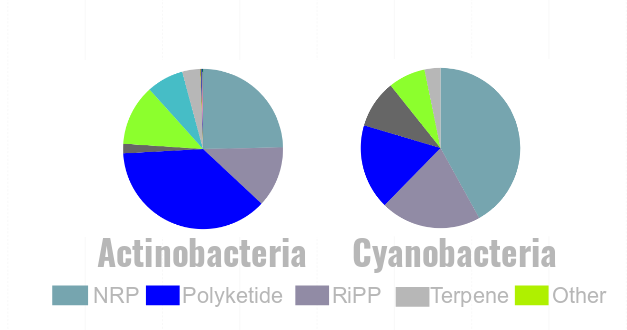
\includegraphics[angle = 0,scale = .7]{chapter2/other.png}
  \caption[Existen cluster biosintéticos no clasificados (other) entre los reportados en MIBiG]{\footnotesize{Existen cluster biosintéticos no clasificados (other) entre los reportados en MIBiG}}
  \label{fig:other}
  \end{figure}
  
  \section{Algoritmos y bases de datos de EvoMining
  2.0}\label{algoritmos-y-bases-de-datos-de-evomining-2.0}
  
  EvoMining está compuesto de dos algoritmos: el primero que utiliza a la
  familia semilla para encontrar todos miembros de la familia entre todos
  los genomas blanco para así detectar genomas donde haya habido
  expansiones e identificar a todos los miembros de la Familia Expandida
  (FE) y luego busca cuáles homólogos seguramente tienen la misma función
  que las secuencias semilla y cuales otros miembros de la familia son más
  similares a genes que han sido reclutados por BGCs de acuerdo a reportes
  previos. El segundo algoritmo permite la visualización de todas las
  copias de una familia expandida en un árbol clasificadas según sus
  posibles destinos metabólicos. Para ello, los algoritmos EvoMining
  necesitan tres bases de datos: i) los genomas blanco, ii) las secuencias
  de enzimas semilla, y iii) la de productos naturales verificados.
  
  \begin{figure}[h!tbp]
  \centering
  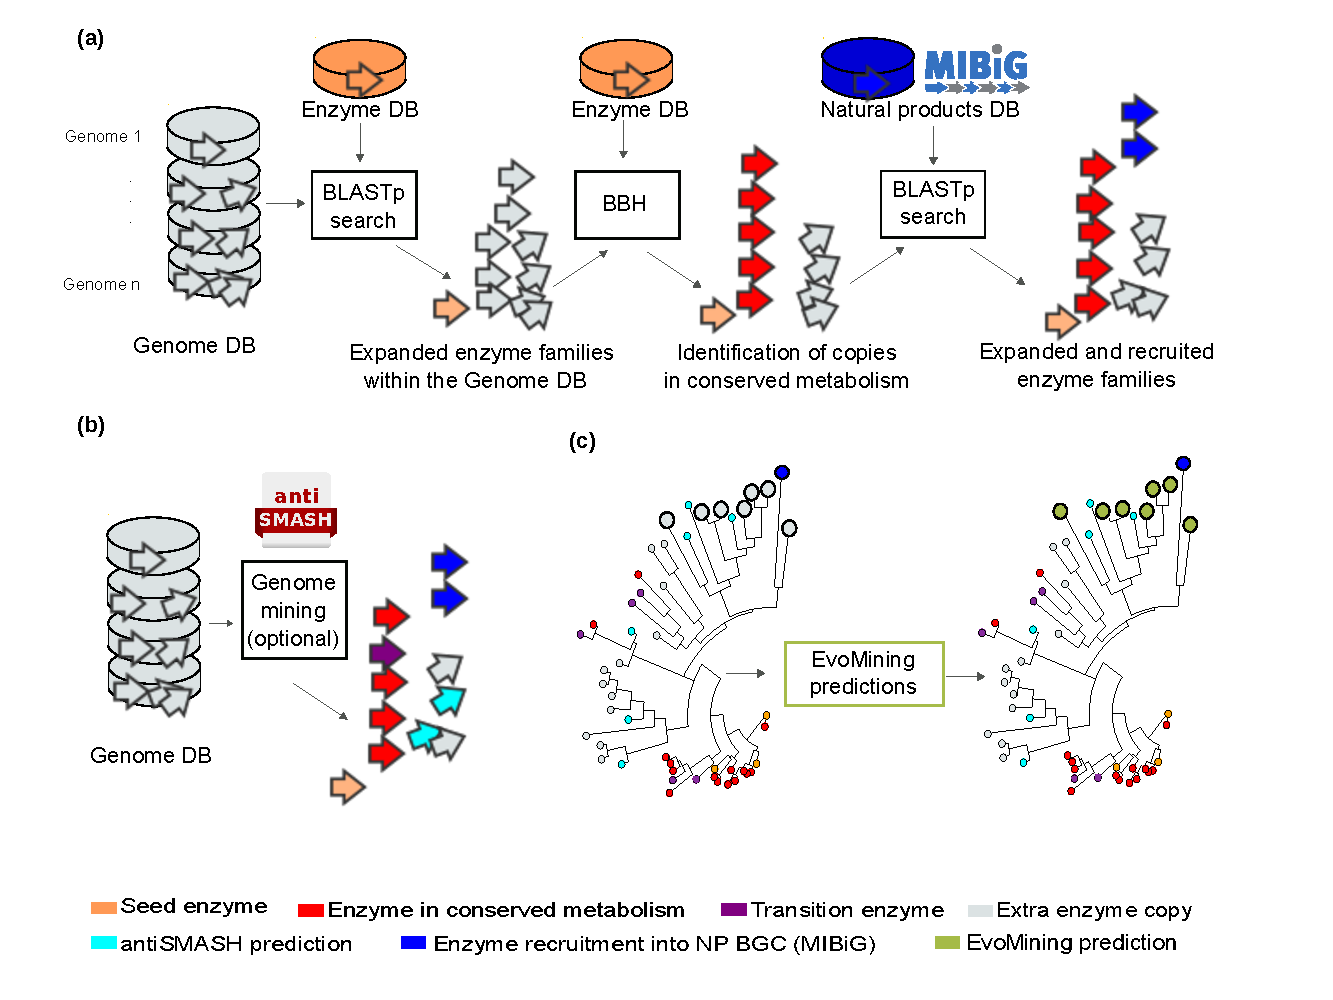
\includegraphics[angle = 0,scale = .8]{chapter2/FigurasPaper/Figure1.pdf}
  \caption[EvoMining Algorithm]{\footnotesize{Representación de la tubería bioinformática de los dos algoritmos que componen EvoMining. a) Algoritmo de expansión - clasificación/reclutamiento. Se ingresan la Enzima DB (cilindro anaranjado) y la Genome DB (cilindros grises) para identificar por medio de BlastP a todos los que sean miembrios de la Familia de las enzimas en Enzima DB, luego se identifican los ortólogos de la base de datos de enzimas (Flechas rojas), finalmente se buscan homólogos de la familia similares a genes reclutados a BGC (Flechas azules),  b) EvoMining toma en cuenta las predicciones de antiSMASH. Cuando un  gen es encontrado como miembro de un BGC predicho por antiSMASH se colorea de cian, o bien de morado si había sido detectado también como parte del metabolismo central (rojo). c) El Algoritmo de visualización muestra un árbol donde cada homólogo de la familia expandida tiene una código de color que lo clasifica como se describe en la leyenda}}
  \label{fig:EvoMiningAlgorithms}
  \end{figure}
  
  \subsection{Algoritmo de expansión y clasificación de grupos de
  homólogos.}\label{algoritmo-de-expansion-y-clasificacion-de-grupos-de-homologos.}
  
  La primera parte de la minería genómica evolutiva de EvoMining consiste
  en detectar las expansiones de la familia semilla y clasificar los
  homólogos que son muy similares a la secuencia de las enzimas con la
  función primaria separándolos de los que son más similares a genes que
  han sufrido reclutamientos a BGC. Este algoritmo requiere las siguientes
  entradas:
  
  \begin{enumerate}
  \def\labelenumi{\alph{enumi})}
  \item
    Secuencia semilla (Enzyme DB). Es una secuencia o un conjunto de
    secuencias de la misma familia que serán interpretadas como las
    enzimas con una función primaria. Por esta razón es importante que el
    usuario haga una curación minuciosa en la que se sugiere que utilice
    genes con evidencia experimental que sí sean de una familia enzimática
    única y conservada. La implementación actual de EvoMining 2.0 permite
    que se introduzcan en el archivo de entrada varias familias bien
    identificadas simultáneamente, sin embargo el algoritmo procesa una
    familia a la vez.
  \item
    Base de datos de genomas blanco (Genome DB). Son las secuencias
    genómicas de todos los organismos en los que se quiera realizar el
    análisis. Se recomienda que los genomas incluidos pertenezcan a un
    mismo linaje taxonómico.
  \item
    Base de datos de genes reclutados a BGC (NP DB). La versión actual
    utiliza MIBiG, que contiene genes de BGC que se han demostrado
    experimentalmente.
  \end{enumerate}
  
  La primera parte de este algoritmo consiste en identificar las Familias
  Expandidas (FE). Una FE consiste en todas las copias detectadas mediante
  una búsqueda con BLASTp, e-value de 0.001 y bitscore de 100, usando como
  \emph{query} las secuencias de aminoácidos de las enzimas semilla
  (Enzyme DB) y como base de datos de búsqueda las secuencias de genomas
  blanco de un linaje taxonómico (Genome DB). En la primera versión de
  nuestro trabajo definimos que un organismo poseía una expansión si el
  número de copias de una familia estaba por encima del promedio mas dos
  desviaciones estándar. Siguiendo esta definición EvoMining colorea en un
  heat plot las expansiones de las familias enzimáticas respecto a un
  linaje taxonómico, señalando explícitamente el número de copias de cada
  familia que se haya agregado como semilla
  (\autoref{fig:ExpansionPatterns} panel b).
  
  Una vez detectados todos los homólogos de la FE sigue encontrar a los
  ortólogos más parecidos a las enzimas semilla de la Enzyme DB mismos que
  son identificados por \emph{Best Bidirectional Hit} (BBH). Estos
  ortólogos serán considerados parte del metabolismo conservado y serán
  posteriormente identificados con color rojo en la visualización. Se
  infiere que son enzimas que tienen la misma función que las semillas.
  Por otra parte, las copias extra de la familia expandida hasta este
  punto son enzimas de las que no se conoce el destino metabólico. Es
  posible que en los pasos subsecuentes de EvoMining sean reconocidas como
  posibles reclutamientos a metabolismo especializado con el uso de
  antiSMASH y MIBiG. En otro caso permanecerán como copias extra con
  destino metabólico desconocido.
  
  El último paso de este algoritmo consiste en encontrar miembros de la
  familia que se encuentren reclutados a BGC reportados anteriormente. En
  este paso definimos un reclutamiento como una copia extra de una familia
  de metabolismo conservado que ahora participa en un \emph{cluster} de
  metabolismo especializado. Ejemplos de reclutamientos conocidos han sido
  observados en BGC reportados en MIBiG. En esta parte, los homólogos de
  la FE que tengan alta similitud con algún gen de MIBiG se clasifican
  como casos de reclutamiento. Una vez obtenidas las FEs expandidas e
  identificado los ortólogos del metabolismo central, se conduce una nueva
  búsqueda con BLASTp, E-value 0.001, utilizando las EFs como
  \emph{queries} contra la base de datos NP DB, la de enzimas
  biosintéticas presentes en BGC. Podrían utilizarse otras bases de datos
  que contengan enzimas con un destino metabólico conocido en lugar de NP
  DB. Hasta este punto se tienen clasificados los genes con la función
  primaria y en este paso se designan los que tendrían una función
  divergente. Es posible agregar un análisis opcional en el que se agregan
  predicciones de los genes que están en BGC de acuerdo a las predicciones
  de antiSMASH. AntiSMASH busca secuencias con dominios conocidos de BGC
  tradicionales en la base de datos de genomas blanco (Genome DB) y además
  busca entre los genes circundantes la presencia de otras enzimas que ya
  hayan sido reclutadas a BGC conocidos. Si alguna enzima de la FE es
  detectada por antiSMASH nos será también útil para identificarla como el
  producto de una expansión que está en proceso o se ha neofuncionalizado.
  La minería genómica tradicional realizada por antiSMASH no es parte de
  la tubería de EvoMining, pero las predicciones de antiSMASH pueden ser
  calculadas previamente por el usuario y utilizadas por EvoMining. En
  este trabajo antiSMASH
  3.0{[}\protect\hyperlink{ref-weber_antismash3_2015}{119}{]} fue
  utilizado en los secuencias de los genomas de la Genome DB
  \autoref{fig:EvoMiningAlgorithms} panel (b).
  
  Los usuarios de EvoMining, por lo tanto, deben definir de antemano las
  familias enzimáticas semilla más apropiadas para un determinado grupo
  taxonómico. El Enzyme DB seleccionado debe contener un conjunto de
  familias donde se puedan detectar los patrones de expansión. A su vez,
  las familias con una distribución restringida a un pequeño porcentaje de
  genomas no son adecuados para el análisis de EvoMining, situación que se
  puede detectar en el heat plot en el primer paso del primer algoritmo de
  EvoMining. También es importante determinar qué familias enzimáticas
  están compartidas por la mayoría de los genomas dentro de los linajes
  genómicos de interés, y si esto es importante para el tipo de análisis
  de EvoMining que se realizarán. El EvoMining DB original incluía las
  familias curadas manualmente que solo incluían enzimas metabólicas
  centrales, pero éstas no representaban el repertorio enzimático central
  de Actinobacteria. Esto se relaciona con la dificultad de definir qué es
  el metabolismo central; por lo tanto, preferimos utilizar el término
  enzimas centrales en diferentes umbrales de conservación. En nuestro
  caso, usamos \(50\%\) para definir las enzimas del \emph{shell}. Esta
  noción implica la posibilidad de automatizar la integración de Enzyme DB
  mediante la selección de familias enzimáticas en cualquier linaje
  genómico dado, evitando la necesidad de definir arbitrariamente qué es
  el metabolismo central.
  
  En conclusión el algoritmo de expansión - clasificación/reclutamiento
  trabaja para identificar tres clases de copias en las familias
  enzimáticas expandidas y tiene como resultado tres salidas. La primera
  es una matriz que contiene el número de genes de cada familia semilla
  por cada genoma que se haya provisto y que puede ser visualizado e
  interpretado independientemente de los otros resultados y procesos de
  EvoMining. La segunda es una tabla por cada FE que enlista todos los
  homólogos pertenecientes a ella así como su identificador de a qué
  categoría pertenece, (i) copias altamente conservadas con algún miembro
  en el metabolismo conservado; (ii) reclutamientos conocidos en BGC de
  productos naturales; y (iii) copias extra que no son reclutamientos
  conocidos ni parte obvia del metabolismo conservado, quedando por
  definir su destino metabólico. La última salida son las secuencias de
  los genes de la FE, que servirán para hacer un análisis de su evolución
  mediante una filogenia en el siguiente algoritmo de visualización.
  
  \subsection{Algoritmo de reconstrucción filogenética y
  visualización}\label{algoritmo-de-reconstruccion-filogenetica-y-visualizacion-1}
  
  Una vez que se tienen definidos los genes de una familia expandida (FE)
  de enzimas y que ya se conoce cuáles de los homólogos realizan la
  función primaria así como los que han sido reclutados a BGC para
  realizar una función divergente, en este algoritmo se visualiza esa
  información junto con la inferencia de los genes que no han sido
  clasificados todavía. Para eso se alinean las secuencias de la FE y se
  construye un árbol filogenético para luego visualizar cada uno de los
  homólogos como una hoja del árbol con un código de color que clasifica
  de acuerdo a la inferencia de origen-destino.
  
  Las secuencias de la FE detectadas por el algoritmo de búsqueda -
  clasificación/reclutamiento se alinean con muscle v3.2 y son curadas con
  Gblocks. Las posiciones ausentes en más del \(50\%\) de las secuencias
  se filtran y remueven del alineamiento final. Para reconstruir
  filogenéticamente la historia de las enzimas se utiliza FastTree
  \(2.1\){[}\protect\hyperlink{ref-price_fasttree_2010}{120}{]} que es un
  método muy rápido pensado para miles de secuencias que utiliza un
  algoritmo definido como ``aproximadamente máxima verosimilitud''. Así se
  obtiene un árbol en formato newick, mismo que puede ser utilizado con el
  software de visualización de
  Microreact{[}\protect\hyperlink{ref-argimon_microreact_2016}{121}{]} y
  que también es usado por EvoMining para ser visualizado en su propia
  plataforma.
  
  Los árboles visualizados en EvoMining diferencian entre la función
  metabólica de cada miembro de una familia génica mediante un código de
  color \autoref{fig:EvoMiningAlgorithms} panel (b, c) . Las secuencias
  más conservadas se identifican mediante BBH contra la Enzyme DB, los
  hits de este proceso son considerados copias de metabolismo central, y
  son marcadas en rojo. En el otro extremo están los reclutamientos
  conocidos con alguna evidencia experimental que fueron reportados en
  MIBiG{[}\protect\hyperlink{ref-medema_minimum_2015}{112}{]}. Estos
  reclutamientos son marcados en azul. Una vez definidos estos dos grupos,
  una predicción de EvoMining es definida como aquellas hojas sin una
  categoría definida en el primer algoritmo y que están más cerca de una
  hoja azul que de una hoja roja. Es decir, son los homólogos que están en
  ramas del árbol que contienen genes descritos como reclutados por BGC y
  que no están en ramas de los homólogos con la función primaria. Estas
  predicciones consideradas con más posibilidades de pertenecer al
  metabolismo especializado que al conservado, son coloreadas en verde
  \autoref{fig:EvoMiningAlgorithms} panel (c).
  
  Además de los tres destinos metabólicos descritos marcados
  respectivamente en rojo, azul y verde, se puede opcionalmente agregar
  información predicha por antiSMASH. Cuando el usuario provee resultados
  de antiSMASH sobre qué genes pertenecen a un BGC que contiene una enzima
  típica de metabolismo especializado, estos se colorean en cían y son
  llamados predicciones antiSMASH. Si una secuencia es al mismo tiempo
  predicción EvoMining y predicción antiSMASH se colorea cían y se ignora
  el verde para enfatizar en los verdes las posibles novedades químicas.
  Cuando una secuencia está en la intersección de las reconocidas como
  metabolismo conservado marcada como roja y predicción de antiSMASH es
  decir color cían entonces es coloreada de púrpura. Estas enzimas de
  intersección entre metabolismo conservado y metabolismo especializado
  son definidas como enzimas de transición ya que se podrían pertenecer al
  metabolismo conservado, al especializado o a ambos. Además las enzimas
  de transición suelen estar en ramas intermedias entre ramas de
  metabolismo conservado y ramas de metabolismo especializado. Finalmente
  para todas las copias extra que no fueron marcadas como rojas, azules,
  verdes, cianes o púrpuras se les asigna el color gris. Así pues gris son
  aquellas hojas del árbol de las que no se tiene un clave sobre su
  destino metabólico, estas secuencias son llamadas de destino metabólico
  desconocido.
  
  En este trabajo se diseñó e implementó el código para hacer el
  visualizador de EvoMining que permite hacer zoom en las ramas de interés
  además de que tiene links en las hojas azules que llevan al BGC en la
  página de MIBiG. También tiene la función de que cuando se seleccionan
  hojas de otro color se expande un recuadro que muestra un mapa del
  contexto genómico de ese homólogo. Finalmente, este algoritmo también
  produce archivos de salida con otros metadatos como el número de copias
  por organismo y para que los árboles producidos por EvoMining sean
  compatible con la visualización de
  Microreact{[}\protect\hyperlink{ref-argimon_microreact_2016}{121}{]}.
  
  \subsection{Actualizaciones de las bases de datos de
  EvoMining}\label{actualizaciones-de-las-bases-de-datos-de-evomining}
  
  Tres bases de datos son requeridas como variables de inicio de
  EvoMining, la primera es el conjunto de secuencias de genomas de un
  linaje, esta base fue llamada Genome DB. La segunda es un grupo de
  secuencias de enzimas de metabolismo conservado llamada Enzyme DB. La
  base de datos se secuencias de genes que pertenecen a un cluster
  biosintético de metabolismo especializado es abreviada como base de
  datos de productos naturales o por sus siglas en inglés NP DB. Las
  transformaciones que sufrieron estas bases de datos desde la primera
  versión de EvoMining hasta este trabajo están resumidas en la tabla uno
  y serán descritas a continuación.
  
  -\textbf{Genome DB} La primera versión tenía 230 genomas de
  Actinobacteria, incluyendo 50 géneros diferentes. Gracias a la explosión
  de datos genómicos disponibles, en EvoMining 2.0 ahora tiene 1245
  genomas, incluyendo 193 géneros diferentes. Así pues, adicional a la
  actualización de Actinobacteria donde fue la primera vez que una prueba
  de concepto de EvoMining fue probada, tres nuevas bases de datos Genome
  DBs fueron integradas, incluyendo Cianobacteria (416 genomas),
  \emph{Pseudomonas} (219 genomas) y Archaea (876 genomas). estas bases
  están disponibles en el repositorio de datos público Zenodo con
  identificador
  \href{https://doi.org/10.5281/zenodo.1219709}{
\includegraphics{chapter2/zenodo_1219709.png}}.
  Estos taxa fueron elegidos por su diversidad de exploración respecto a
  BGC, por ejemplo Actinobacteria posee 602 MIBiG BGC, Cianobacteria
  cuenta con 60 MIBiG BGC y \emph{Pseudomonas} 53 MIBiG BGC. Estos tres
  taxa han sido ampliamente explorados experimentalmente y su riqueza
  metabólica está fuera de duda; en contraste Archaea sólo posee 1 BGC en
  la nueva versión MIBiG (v.1.4), y no había ninguno al tiempo de la
  realización de este trabajo (v.1.3). Por esta razón, incluir el dominio
  Archaea en los análisis permitía explorar espacios metabólicos
  previamente ignorados en la minería genómica.
  
  Las predicciones de EvoMining se basan en identificar expansiones de
  familias de enzimas en lugar de buscar BGC completos, por esta razón los
  borradores de genomas con un promedio de al menos 5 genes por contig
  también pudieron ser incluidos en la base de datos Genome DB. Los
  genomas elegidos fueron recopilados de la base de datos pública NCBI tal
  y como estaba disponible en Enero de 2017. Las secuencias de DNA de
  estos genomas fueron anotadas como aminoácidos por la plataforma
  RAST{[}\protect\hyperlink{ref-overbeek_seed_2014}{92}{]} que a su vez
  realiza anotaciones funcionales basadas en la homología con otras
  secuencias con funciones descritas. Estos genomas, previo al análisis de
  EvoMining fueron minados por
  antiSMASH{[}\protect\hyperlink{ref-weber_antismash3_2015}{119}{]} con un
  parámetro \texttt{cf\_threshold\ de\ 0.7}. Estos resultados fueron
  suministrados como una base de datos interna, la antiSMASH DB para
  finalmente esta información ser incorporada a los árboles de EvoMining.
  
  -\textbf{Enzyme DB} La versión previa de la base de datos de EvoMining
  Enzyme DB comprendía 106 FEs, de metabolismo central de acuerdo a
  reconstrucciones metabólicas de los organismos \emph{Streptomyces
  coelicolor}, \emph{Mycobacterium tuberculosis} y \emph{Corynebacterium
  glutamicum}
  {[}\protect\hyperlink{ref-cruz-morales_phylogenomic_2016}{61}{]}. Estos
  106 EFs comprenden 339 secuencias de aminoácidos de Actinobacteria, que
  fueron usadas como secuencias semilla. En la versión actual, las 106
  familias fueron filtradas hasta quedar sólo 42 que están presentes en
  Cianobacteria, \emph{Pseudomonas} y Archaea. Durante el proceso de
  selección se escogieron genomas semilla que estuvieran contenidos en un
  sólo contig para evitar excluir familias debido a huecos debidos a
  problemas técnicos relacionados a la secuenciación o al ensamble de los
  genomas. Los genomas semillas son los proveedores de las secuencias
  semilla que conforman la base de datos Enzyme DB. Para Cyanobacteria,
  los genomas seleccionados son \emph{Cianothece} sp. ATCC 51142 ,
  \emph{Synechococcus} sp. PCC 7002 y \emph{Synechocystis} sp. PCC 6803;
  para el género \emph{Pseudomonas}, se escogieron \emph{Pseudomonas
  fluorescens} pf0-1, \emph{Pseudomonas protegens} Pf5, \emph{Pseudomonas
  syringae} y \emph{Pseudomonas fulva} 12-X; y para el dominio Archaea,
  los elegidos son \emph{Natronomonas pharaonis}, \emph{Methanosarcina
  acetivorans}, \emph{Sulfolobus solfataricus} y \emph{Nanoarchaeum
  equitans} Kin4-M. Las enzimas semilla que conforman la base Enzyme DB,
  fueron determinadas en los genomas semilla de cada linaje mediante BBH
  contra la base de datos de secuencias de metabolismo conservado original
  de EvoMining, la Actinobacteria Enzyme DB
  {[}\protect\hyperlink{ref-cruz-morales_phylogenomic_2016}{61}{]}. La
  herramienta Metaphor
  {[}\protect\hyperlink{ref-van_der_veen_metaphor_2014}{81}{]} fue
  implementada para obtener los BBH, se filtraron aquellas secuencias con
  menos del \(30\%\) de identidad en un alineamiento del \(80\%\) de la
  secuencia de las dos proteínas. Como resultado, las 106 familias de
  Actinobacteria quedaron reducidas a 42 FEs, compartidas por los genomas
  semilla de Actinobacteria, Cianobacteria, \emph{Pseudomonas} y Archaea.
  Las bases de datos Enzyme DBs de todos los linajes están disponibles en
  Zenodo con número de identificación
  \href{https://doi.org/10.5281/zenodo.1219709}{
\includegraphics{chapter2/zenodo_1219709.png}}
  
  -\textbf{NP DB} (Base de datos de genes biosintéticos de productos
  naturales). Los primeros análisis realizados con EvoMining incluían un
  base de datos de productos naturales NP DB de 226 BGC reunidos de la
  literatura y curados manualmente
  {[}\protect\hyperlink{ref-cruz-morales_phylogenomic_2016}{61}{]}. En
  este trabajo la base NP DB que se utilizó para los análisis es MIBiG
  v1.3{[}\protect\hyperlink{ref-medema_minimum_2015}{112}{]}. La base que
  viene incluida con el contenedor de EvoMining fue actualizada a la
  siguiente versión MIBiG v.1.4 liberada en Agosto de 2018. Esta nueva
  versión comprende 1813 NP BGC y un total de \(31,023\) secuencias de
  proteínas.
  
  \section{EvoMining detecta distintas dinámicas evolutivas de las enzimas
  metabólicas que dependen de la familia enzimática y del linaje
  taxonomíco.}\label{evomining-detecta-distintas-dinamicas-evolutivas-de-las-enzimas-metabolicas-que-dependen-de-la-familia-enzimatica-y-del-linaje-taxonomico.}
  
  \subsection{Los perfiles de expansión de las proteínas dependen del
  linaje.}\label{los-perfiles-de-expansion-de-las-proteinas-dependen-del-linaje.}
  
  Para entender la evolución de las enzimas y rutas metabólicas se
  seleccionaron cuatro linajes de diversas características los phyla
  Actinobacteria y Cianobacteria , el género \emph{Pseudomonas} y el
  dominio Archaea. Todos los resultados en las figuras son presentados en
  este orden. Estos taxa fueron seleccionados para tener un espectro de
  análisis que abarcara tanto microorganismos ampliamente reconocidos como
  productores de NP, es decir Actinobacteria (602 MIBiG BGC),
  Cyanobacteria (60 MIBiG BGC) y \emph{Pseudomonas} (53 MIBiG BGC); como
  también Archaea (0 BGC en MIBiG versión 1.3), que representa un dominio
  poco explorado en lo que respecta a los genes que forman parte de
  metabolismo especializado
  {[}\protect\hyperlink{ref-charlesworth_untapped_2015}{122}{]}.
  
  Basándonos en estas bases de datos de genomas blanco (Genome DB), como
  es explicado en la \autoref{fig:SeedGenomes} panel (a), un conjunto de
  familias enzimáticas comunes fue identificado. Notablemente, de las 106
  familias actinobacteriales menos del 50\% están conservadas en los
  nuevos taxa. Cada base de datos, una para cada taxon, contiene sólo 42
  FEs (Table S1). La observación de que 64 FEs no están conservadas en los
  cuatro taxa refleja lo específico del metabolismo en cada linaje con
  respecto a los otros
  {[}\protect\hyperlink{ref-jordan_lineage-specific_2001}{123}{]}.
  
  Ya que la cantidad de expansiones de un gen en un organismo sería
  proporcional al tamaño de su genoma, verificamos cómo cambia el número
  de copias de los genes que pertenecen a las 42 FEs conservadas con
  respecto al tamaño de los genomas en los cuatro linajes. Todos los
  linajes tienen patrones de expansión similares en las 42 FEs analizadas
  hasta un tamaño de genoma 5 Mbp. En genomas más grandes, el número total
  de secuencias crece más en \emph{Pseudomonas} que en el phylum
  Actinobacteria, que a su vez es más grande que el phylum Cianobacteria y
  que el dominio Archaea \autoref{fig:SeedGenomes} panel(b). Se observa
  cómo \emph{Pseudomonas} es el linaje en el que su tamaño de genoma crece
  tanto como el número de copias de genes de familias muy conservadas
  (Glucólisis, síntesis de aminoácidos, Ciclo de Krebs, etc.). El
  resultado en Archaea se debe a que no se han descubierto organismos
  tamaños de genoma Archaea de tamaño comparable a los de
  \emph{Streptomyces} o \emph{Pseudomonas} (\(> 5\)Mbp). Actinobacteria y
  Cianobacteria aunque tienen genomas \(>5\)Mbp, el incremento en tamaño
  podría ser porque tienen expansiones de genes que no son del metabolismo
  más conservado, porque obtienen más genes por transferencia horizontal u
  otros mecanismos por los que se incremente el tamaño del genoma.
  Cianobacteria a pesar de tener genomas grandes no tiene tantas
  expansiones en estas FEs Esta observación, es posible que sea
  generalizable a todas las FEs de metabolismo conservado o bien que se
  deba a un sesgo en la selección de las familias que componen a las FEs.
  
  \begin{figure}[h!tbp]
  \centering
  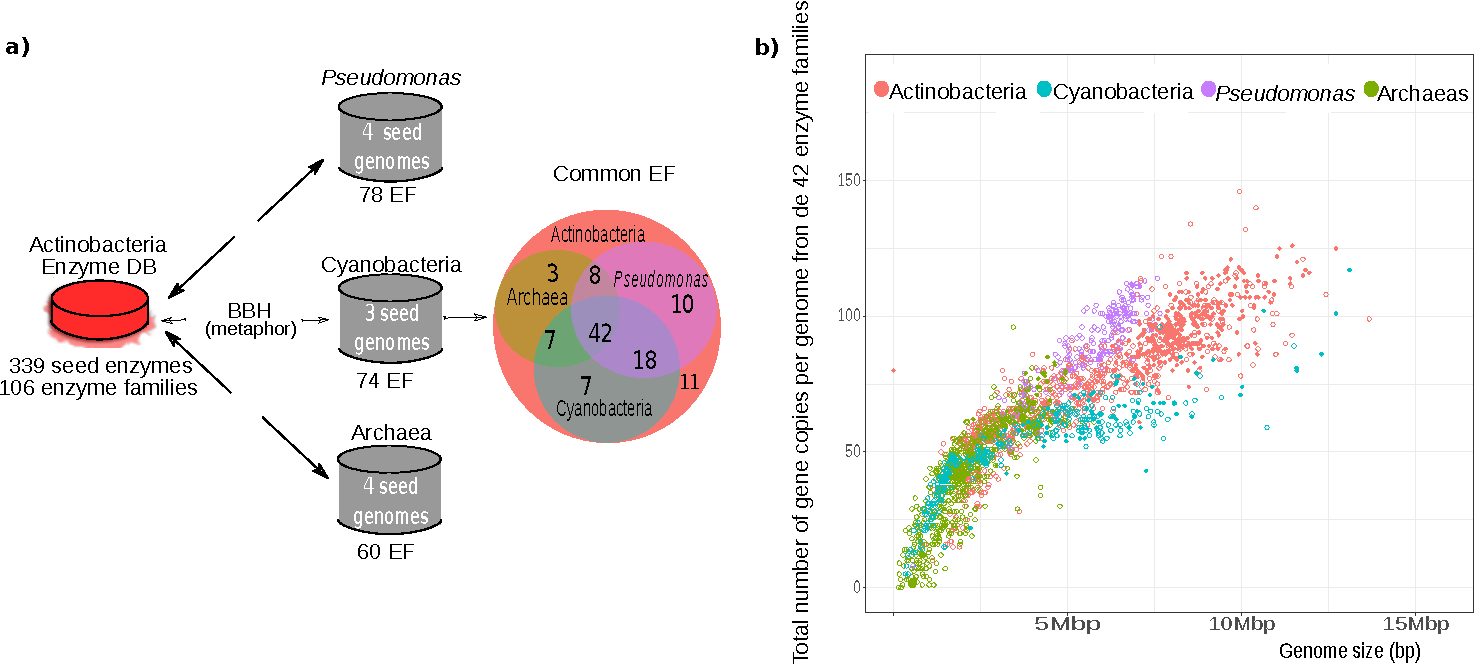
\includegraphics[angle = 0,scale = .6]{chapter2/FigurasPaper/Figure2.pdf}
  \caption[Contrucción de la base de datos Enzyme DB de enzimas semilla.]{\footnotesize{ EvoMining Enzyme DB. (a) La base de datos de enzimas de la versión previa de EvoMining se filtró para establecer un conjunto común de 42 familias enzimáticas conservadas para los phyla Actinobacteria y Cyanobacteria, el género $Pseudomonas$ y el dominio Archaea. (b) Todos los taxones muestran expansiones de familias enzimáticas que correlacionan con el tamaño del genoma. Las diferencias en las tasas de expansión entre los taxones se observan principalmente después de un tamaño de genoma superior a 5 Mbp. En este umbral, $Pseudomonas$ supera las expansiones de Actinobacteria, que a su vez supera a Cyanobacteria en las 42 familias seleccionadas.}}
  \label{fig:SeedGenomes}
  \end{figure}
  
  Los órdenes con mayor número de copias fueron en las expansiones de las
  familias de la Enzyme DB fueron \emph{Streptomycetales} y
  \emph{Nostocales}, en Actinobacteria y Cianobacteria respectivamente.
  Esta observación es congruente con que estos órdenes tienen un tamaño de
  genoma grande en sus linajes correspondientes, y además están
  ampliamente representados en MIBiG como sintetizadores de productos
  naturales. Interesantemente la clase Halobacteria es la que muestra
  mayor número de expansiones en Archaea, aunque no es la clase con mayor
  tamaño de genoma en promedio \autoref{fig:SizeGenomes}.
  
  \begin{figure}[h!tbp]
  \centering
  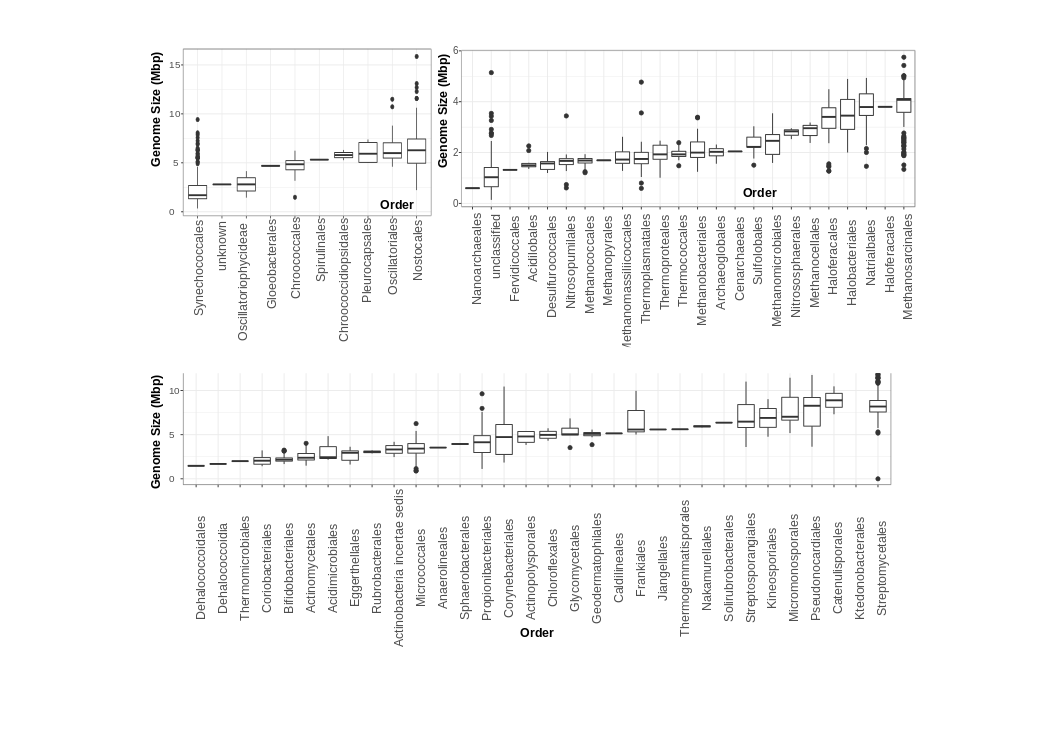
\includegraphics[angle = 0,scale = .5]{chapter2/Genomesize.png}
  \caption[Tamaño de genoma en órdenes de Actinobacteria y Cianobacteria y en clases De Archaea.]{\footnotesize{Tamaño de genoma en órdenes de Actinobacteria y Cianobacteria y en clases De Archaea. Actinobacteria y Cianobacteria tienen algunos genomas con tamaños superiores a 6 Mbp, que es el máximo que se encuentra en Archaea. El tamaño promedio en el género $Pseudomonas$ es de 5.8 MBbp con un máximo de 7.6Mbp entre los genomas utilizados en este trabajo.
  (no se muestra en la figura)}}
  \label{fig:SizeGenomes}
  \end{figure}
  
  Esta observación es congruente con que las archaeocinas,
  dicetopiperazinas, carotenoides y otros productos naturales de Archaea
  fueron aislados de especies de Halobacteria, los genes, probablemente en
  BGC, que sintetizan de estos metabolitos no han sido caracterizados
  {[}\protect\hyperlink{ref-charlesworth_untapped_natural_products_Archaea_2015}{86}{]}.
  Por ello EvoMining una herramienta de minería genómica que puede ayudar
  a explorar linajes poco minados con el potencial de descubrir nuevas
  rutas metabólicas.
  
  Es claro que en las familias conservadas seleccionadas el número de
  copias extra correlaciona con el tamaño de genoma los perfiles de
  expansiones son diferentes en cada grupo taxonómico y que este
  incremento parece cambiar su patrón en todos los linajes a partir de
  5Mbp \autoref{fig:SeedGenomes} (2b). Por ello se concluye que para
  ensamblar una base de datos genómica para EvoMining se debe considerar
  que las expansiones dependen tanto de los distintos linajes taxonómicos
  como de la diversidad del tamaño de genoma.
  
  \subsection{\texorpdfstring{El \emph{shell} genome posee expansiones en
  sus familias
  enzimáticas}{El shell genome posee expansiones en sus familias enzimáticas}}\label{el-shell-genome-posee-expansiones-en-sus-familias-enzimaticas}
  
  La figura muestra que \emph{Pseudomonas} posee en promedio más copias
  por genoma que los otros taxa. De las 42 familias analizadas el
  \(54.8\%\) tiene su máximo número promedio de copias por genoma en este
  linaje. \autoref{fig:DataTabla42} . En contraste, Actinobacteria es el
  máximo en \(26.2\%\) de las FEs, mientras que Archaea y Cianobacteria
  empatan en ser el linaje con expansiones sólo en el \(9.5\%\) de los
  casos. Aunque existen familias como la acetylornitino aminotransferasa o
  la acetolactato sintasa (ALS) que están expandidas en todos los linajes
  (coordenadas A1 y E1, \autoref{fig:DataTabla42},
  \autoref{fig:42Expansiones} ). En esta figura, para cada familia en los
  ejes horizontales siempre se muestran en orden cuatro barras:
  Actinobacteria, Cianobacteria, \emph{Pseudomonas} y Archaea. El código
  de color es el mismo que el de los árboles de EvoMining, con excepción
  del verde, pues aun no hay árbol filogenético. Así pues es como sigue:
  rojo para el metabolismo conservado, azul para los reclutamientos
  anotados en MIBiG, cían para predicciones de antiSMASH de pertenencia a
  un BGC de metabolismo especializado, púrpura para la intersección entre
  el metabolismo conservado y predicciones antiSMASH y gris para
  expansiones sin destino metabólico conocido. La letra en la parte
  inferior y los números a la izquierda son coordenadas para facilitar la
  identificación de la familia en la Tabla S1. Los triángulos indican el
  linaje con el mayor número de copias por genoma en promedio, y los
  círculos representan la menor cantidad de copias. Aunque Archaea tiende
  a ser los taxones menos expandidos, esta tendencia revierte en las
  familias A4, C4, G4 (GDH) y B5. GDH y ALS (E1) están encerradas en una
  cuadro, estas enzimas son el origen de los reclutamientos en el BGC de
  escitonemina. Muchas otras familias exhiben expansiones sólo en ciertos
  linajes. Tal es el caso de la fumarato reductasa subunidad de
  hierro-azufre, cordenada C3 de la figura, muy expandida en
  Actinobacteria pero con menos de una copia por genoma en promedio en
  Cianobacteria.
  
  \begin{figure}[h!tbp]
  \centering
  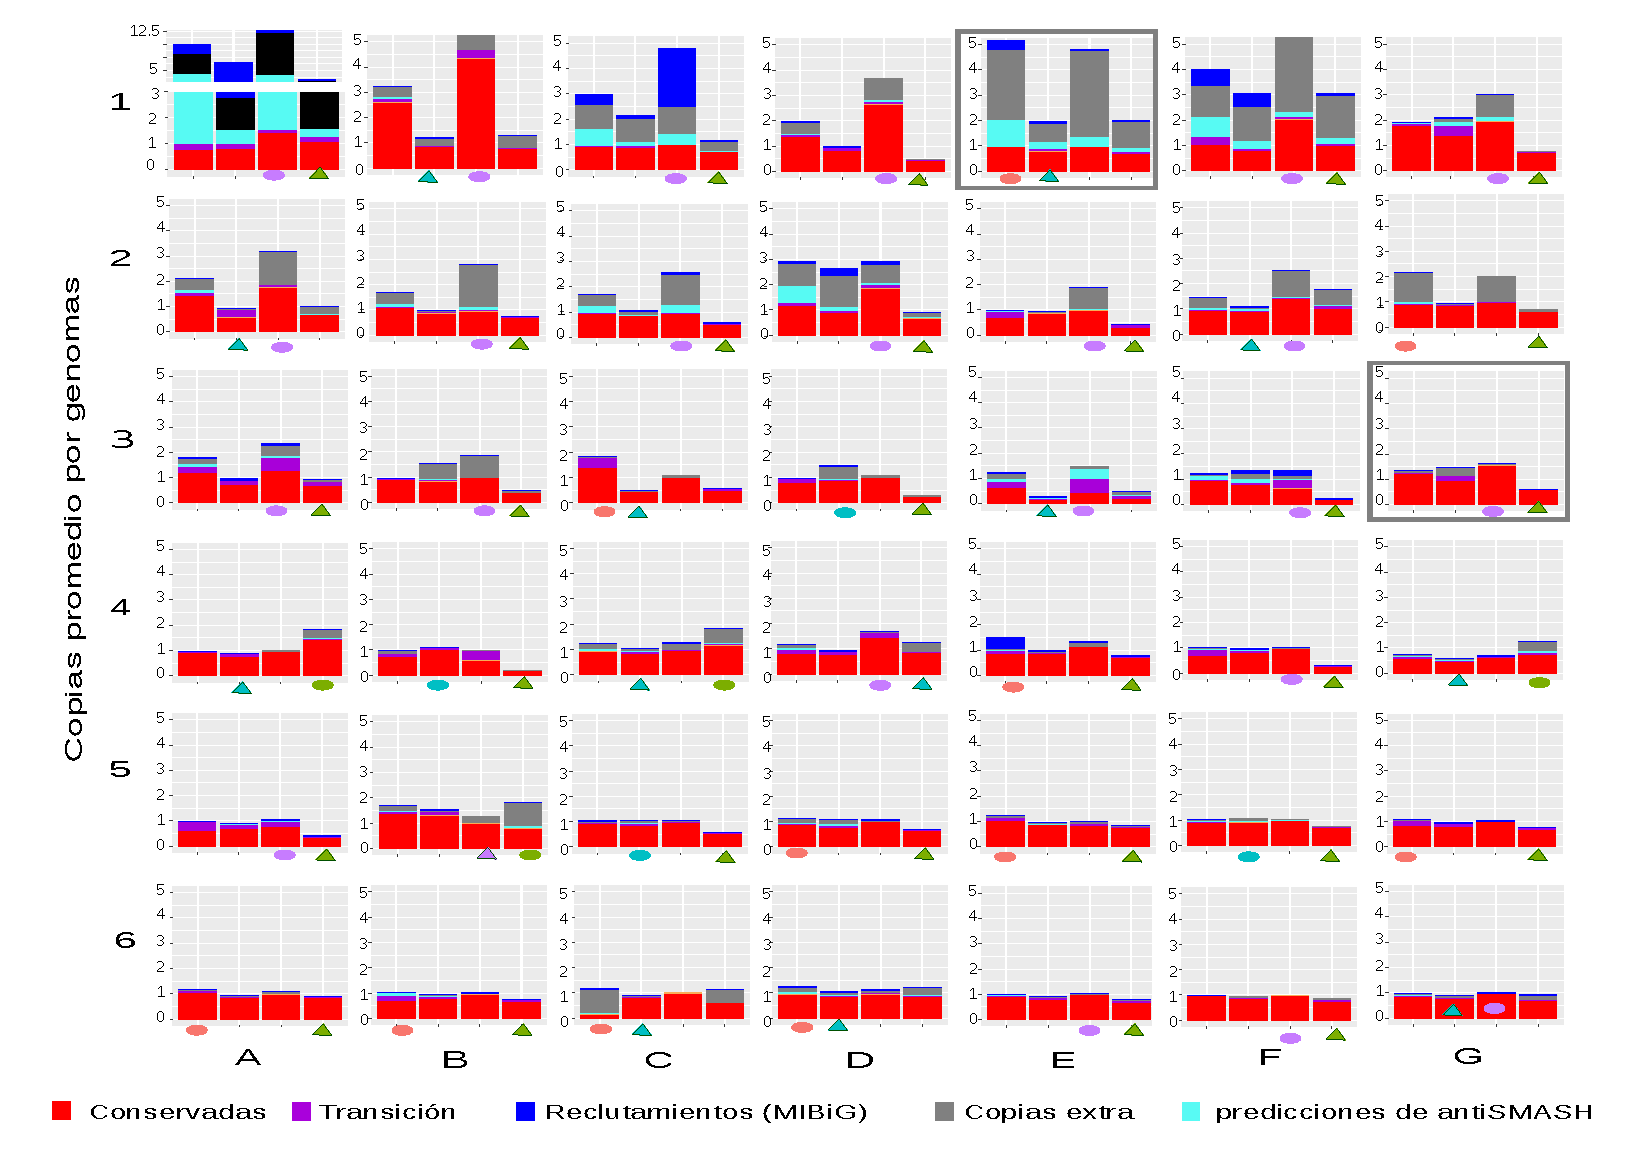
\includegraphics[angle = 0,scale = .6]{chapter2/FigurasPaper/Figure3S.pdf}
  \caption[Expansiones de las 42 enzimas comunes en Actinobacteria, Cyanobacteria, $Pseudomonas$ y Archaea]{\footnotesize{Perfiles de EvoMining  de las 42 enzimas conservadas en linajes genómicos seleccionados. Las coordenadas en forma de letras A-G y los números 1-6 se muestran en esta figura para
  Localice fácilmente la familia y sus propiedades en la Tabla S1.}}
  \label{fig:42Expansiones}
  \end{figure}
  
  No todas las FEs están expandidas, aunque las 42 familias conservadas
  están presentes en alguno de los genomas semilla de cada linaje, varias
  de ellas no se encuentran en la mayoría de los genomas del resto de su
  base de datos. Este es el caso de AroB en Archaea, donde tiene muy poca
  representación. Sin embargo, un gran porcentaje de familias muestra
  perfiles de expansión acordes a la tendencia del número total de copias
  extra, \autoref{fig:DataTabla42}. Por familia, \emph{Pseudomonas} suele
  ser el linaje con el mayor número de expansiones mientras que Archaea
  suele ser el linaje menos expandido. Entre las excepciones a esta
  tendencia está GDH una familia incluida dentro de los ocho casos
  seleccionados. Para ilustrar esta diversidad que son mostrados en la
  figura \autoref{fig:ExpansionPatterns}
  
  panel (a). En esta figura los máximos están marcados con un círculo
  mientras que los mínimos con un triángulo, los colores de estas formas
  geométricas representan los mismos linajes que los mostrados en la
  \autoref{fig:SeedGenomes}. Del total de las 42 familias, GDH es una de
  las cuatro FEs en las que el mayor número de expansiones se encuentra en
  Archaea. De hecho, GDH tiene menos de una copia por genoma en promedio
  en los otros taxa, probando que no se encuentra dentro del \emph{core}
  genómico de estos linajes. Esto contrasta con AroB, que muestra una
  tendencia opuesta, no es parte del \emph{core} de Archaea pero muestra
  copias extra y una presencia mayor que uno en promedio en los otros tres
  taxa analizados \autoref{fig:ExpansionPatterns} panel (b). Los ocho
  casos mostrados en la figura son todos parte de un cluster biosintético
  de Cianobacteria, descrito en las secciones posteriores de este trabajo.
  
  \begin{figure}[h!tbp]
  \centering
  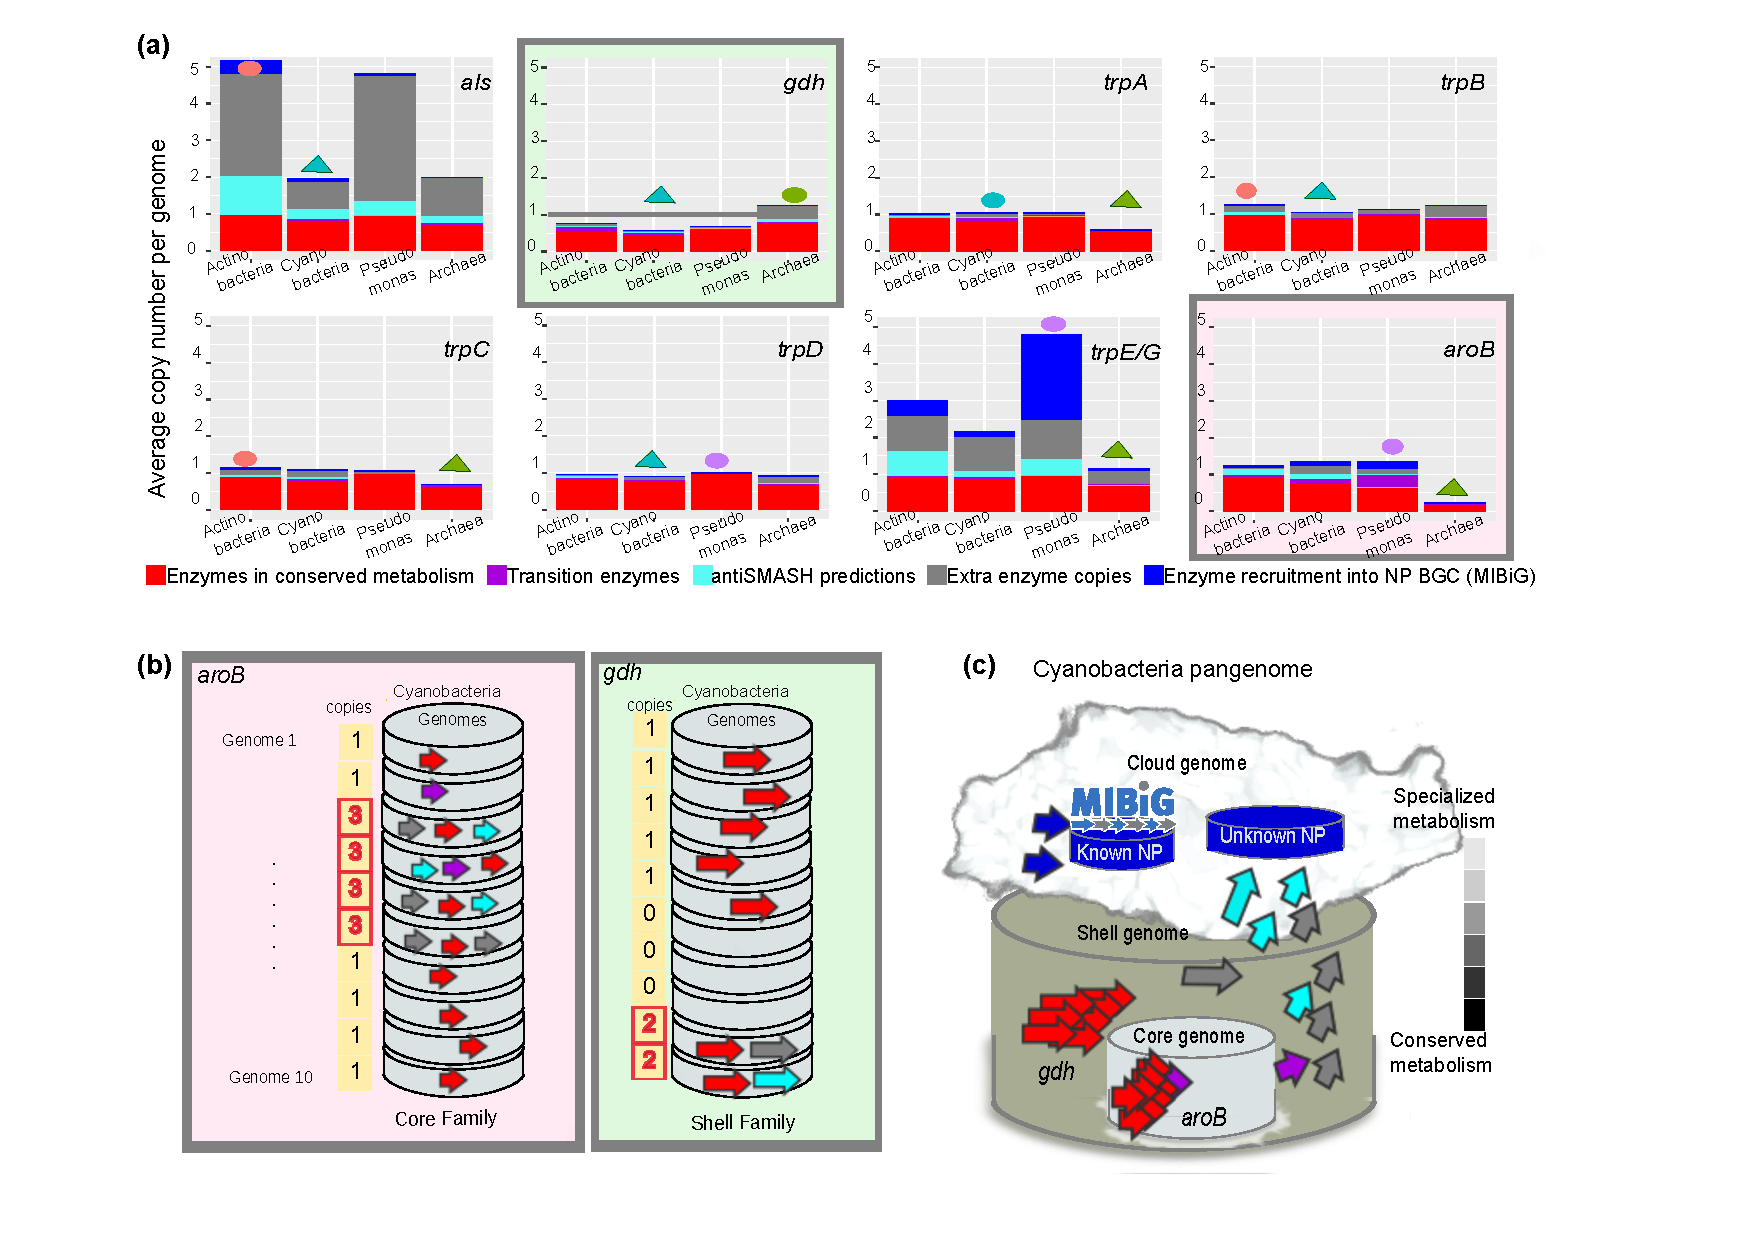
\includegraphics[angle = 0,scale = .6]{chapter2/FigurasPaper/Figure3.pdf}
  \caption[Patrones de expansión de familias que participan en la síntesis de escitonemina]{\footnotesize{Perfiles de expansiones de EvoMining de enzimas conservadas seleccionadas. (a) Patrones de expansión de las ocho familias conservadas cuyas copias adicionales participan en la biosíntesis de escitonemina. El conjunto completo de 42 EF se muestra en la figura anterior. La codificación de colores es la siguiente: rojo para el metabolismo conservado, azul para los reclutamientos anotados en MIBiG, cian para las predicciones antiSMASH de metabolismo especializado, púrpura para la intersección entre el metabolismo conservado y las predicciones antiSMASH, y gris para las expansiones sin destino metabólico conocido. El orden en el eje x es Actinobacteria, Cianobacteria, $Pseudomonas$ y Archaea. Los triángulos indican el linaje con el mayor número de copias por genoma en promedio, y los círculos representan el linaje menos expandido. Aunque Archaea tiende a ser los taxones menos expandidos, esta tendencia se revierte en la familia GDH. (b) Se proporciona un ejemplo de un $core$ frente a una familia enzimática $shell$. AroB es un EF básico porque tiene al menos una copia por genoma, mientras que GDH es un familia del $shell$ debido a su ausencia en tres genomas. A pesar de ser una familia $shell$, GDH tiene copias adicionales que pueden ser reclutadas en un metabolismo especializado. (c) Modelo para la $nube$ o genoma variable compuesto parcialmente por enzimas que pertenecen a BGC de productos naturales. En este modelo, el metabolismo conservado se compone de familias tanto del $shell$ como del $core~genome$. Estas familias pueden sufrir eventos de expansión, y algunas de las copias adicionales son reclutadas para realizar nuevas funciones en el metabolismo especializado.}}
  \label{fig:ExpansionPatterns}
  \end{figure}
  
  Con estas observaciones sospechamos que GDH es miembro del \emph{shell
  genome} (Ver capítulo 1)
  {[}\protect\hyperlink{ref-koonin_genomics_2008}{124}{]} en los taxa
  Actinobacteria , Cianobacteria y \emph{Pseudomonas}, ya que en promedio
  está cerca de tener una copia promedio por genoma. El promedio no es
  suficiente para decir que una familia pertenece al \emph{shell}, podrían
  suceder casos sobre todo cuando hay mucha variación en un taxon como en
  el caso de un domino o un phylum en contraposición con taxones
  conservados como géneros en los que para una cierta familia la mitad de
  los genomas de un linaje tuviera dos copias y la otra mitad cero. Sin
  embargo en el caso de la GDH si es consistente en que está presente en
  más del \(50\%\) de los genomas de cada linaje
  \autoref{fig:ExpansionPatterns} panel (a). Las modas de número de copias
  también son informativas, una sola copia extra puede ser la que sea
  reclutada en metabolismo especializado.
  
  En la figura \autoref{fig:ExpansionPatterns} se muestra un ejemplo donde
  AroB es una enzima \emph{core} en oposición a GDH que es una enzima
  \emph{shell}. En este esquema conceptual, en algunos de los genomas que
  contienen a AroB existen copias que se dedican al metabolismo
  especializado marcadas en color cían, otras copias no tienen un destino
  metabólico conocido por lo que están marcadas en gris, y otras más
  marcadas en púrpura son enzimas de transición que están llevando a cabo
  simultáneamente una función en metabolismo central y otra en metabolismo
  especializado. En contraste a AroB se muestra GDH, que a pesar de no
  tener copias en algunos genomas y con un promedio de copias por genoma
  menor a uno y una moda de uno en esta muestra, GDH existe por duplicado
  en dos genomas. En uno de esos genomas donde GDH tiene una copia extra,
  más allá de la moda, esa copia se muestra como un reclutamiento al
  metabolismo especializado en cían. \autoref{fig:ExpansionPatterns} panel
  (b) .
  
  Las expansiones encontradas por EvoMining en la familia GDH incluían
  predicciones de antiSMASH para Actinobacteria, Cianobacteria y Archaea,
  no así para \emph{Pseudomonas}. La secuencia del reclutamiento de GDH
  por los \emph{clusters} biosintéticos escitonemina y el policétido
  pactamycin {[}\protect\hyperlink{ref-kudo_cloning_2007}{125}{]}, es
  suficientemente parecida como para que EvoMining la detecte como
  expansión en Actinobacteria, Cianobacteria y Archaea, pero es tan
  divergente respecto a la familia GDH en \emph{Pseudomonas} que EvoMining
  lo deja fuera de la familia expandida en este linaje. Los árboles donde
  puede apreciarse esta observación pueden consultarse más adelante en la
  \autoref{fig:GenomicLinajes} de la siguiente sección.
  
  Los resultados anteriores sugieren que la evolución del metabolismo
  especializado es linaje dependiente, y más aún que tal y como ya se
  conocía en las FEs del \emph{core genome} las enzimas del \emph{shell}
  como GDH también poseen el potencial de ser reclutadas en NP BGC. A
  partir de estos resultados \autoref{fig:ExpansionPatterns} paneles
  (a,b), se realizó un esquema conceptual para explicar cómo en linajes
  genómicos diversos las familias de enzimas con origen en el metabolismo
  central que forman parte del \emph{core genome} o bien las familias en
  el metabolismo conservado que incluye tanto al \emph{core} como al
  \emph{shell genome}, evolucionan al metabolismo especializado que tiene
  una mayor representación en el \emph{cloud genome}
  \autoref{fig:ExpansionPatterns} panel (c) . Este modelo es relevante
  porque establece el papel de las familias del \emph{shell genome}, que
  no fue considerado en la primera iteración que explotó las capacidades
  de EvoMining como herramienta de minería genómica para encontrar BGC
  novedosos{[}\protect\hyperlink{ref-navarro-munoz_computational_2018}{110}{]}.
  
  \begin{figure}[h!tbp]
  \centering
  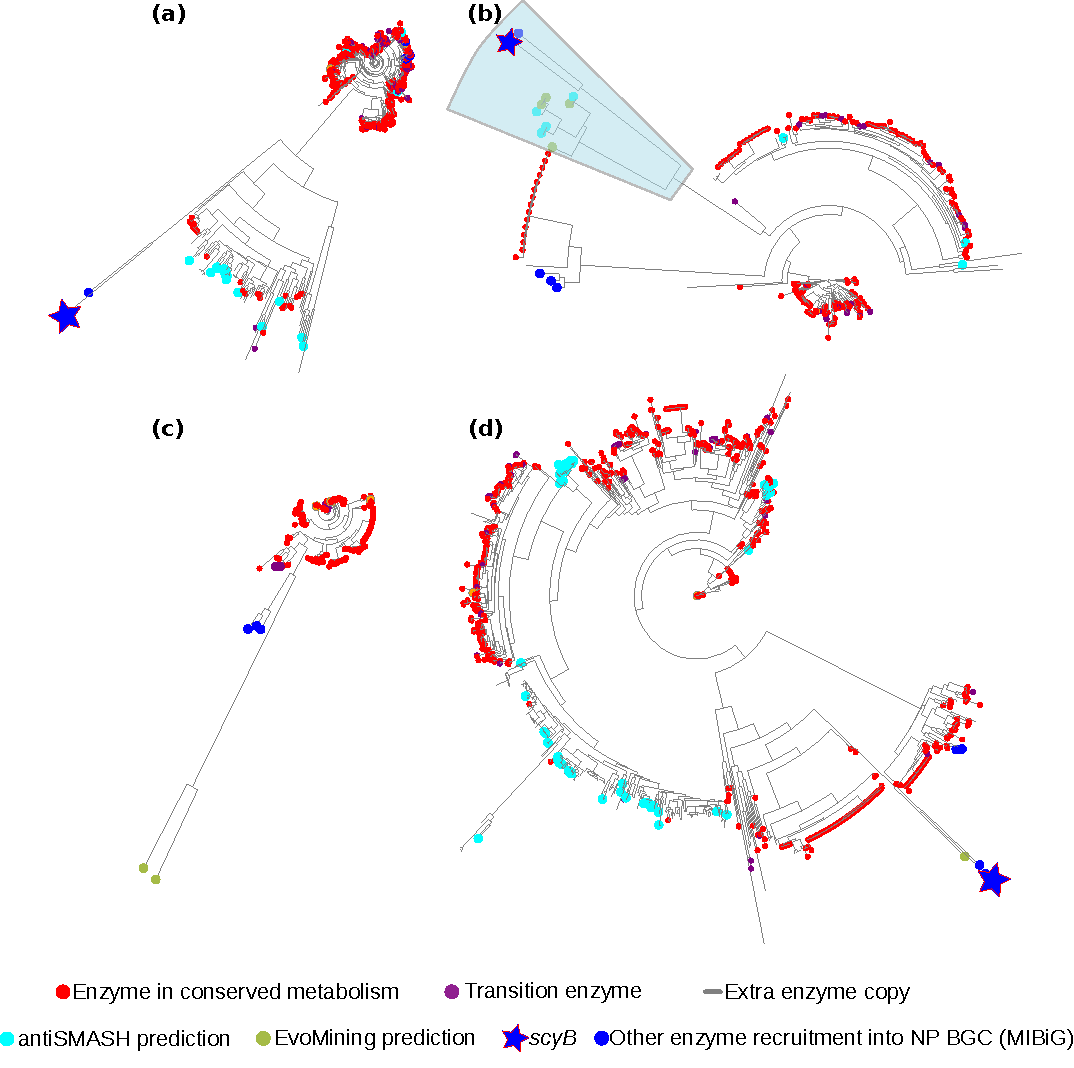
\includegraphics[angle = 0,scale = .8]{chapter2/FigurasPaper/Figure4.pdf}
  \caption[Árboles de EvoMining de glutamato deshidrogenasa en cuatro linajes genómicos]{\footnotesize{Árboles de EvoMining de glutamato deshidrogenasa en cuatro linajes genómicos. (a) Reconstrucciones filogenéticas específicas del linaje que muestran claras diferencias en los perfiles de expansión en Actinobacteria, Cyanobacteria, $Pseudomonas$ y Archaea. Actinobacteria no tiene predicciones de EvoMining, ya que su rama de expansión principal carece de reclutamientos de MIBiG. Sin embargo, es posible que se produzca un metabolito especializado dentro de esas copias de destino desconocido (gris). (b) El árbol de Cyanobacteria posee cuatro predicciones de EvoMining y cuatro de antiSMASH. $scyB$ se encuentra junto a esta rama del metabolismo especializado. (c) La mayoría de las copias de $Pseudomonas$ están etiquetadas como metabolismo conservado, con solo dos predicciones de EvoMining ubicadas en una rama divergente. $Pseudomonas$ tiene un promedio de copias por genoma menor que uno en esta familia lo que se refleja en que casi todas las copias fueron etiquetadas como metabolismo central. (d) Archaea, el taxón más expandido, tiene una rama poblada con expansiones etiquetadas como hits de antiSMASH (cian), pero sin ninguna predicción de EvoMining. Los cuatro linajes tienen reclutamientos de MIBiG, pero $scyB$ solo fue reconocido por Actinobacteria, Cyanobacteria y Archaea. }}
  \label{fig:GenomicLinajes}
  \end{figure}
  
  En la siguiente sección se analizarán los patrones de expansión
  reclutamiento de GDH provistas por EvoMining para GDH y se describirán
  los árboles filogenéticos de cada linaje mostrados en la
  \autoref{fig:GDHGenomicLineages} , así como un árbol que incluye
  conjuntamente secuencias de todos los linajes \autoref{fig:GDHJunto} .
  En Archaea, GDH tiene en promedio 1.23 copias por genoma, mientras en
  Actinobacteria, Cianobacteria y \emph{Pseudomonas} esta media es de
  0.74, 0.56 y 0.65, respectivamente. En estos tres taxa GDH es parte del
  \emph{shell genome} \autoref{fig:DataTabla42}. Además de GDH se
  estudiaron las expansiones y los árboles filogenéticos de TrpA, TrpB,
  TrpC, TrpD, TrpEG, AroB y ALS, todas ellas parte de las 42 FEs
  conservadas entre los cuatro linajes y a la vez reclutadas en
  escitonemina
  {[}\protect\hyperlink{ref-balskus_investigating_2008}{115}{]} un cluster
  biosintético de Cyanobacteria.
  
  \begin{figure}[h!tbp]
  \centering
  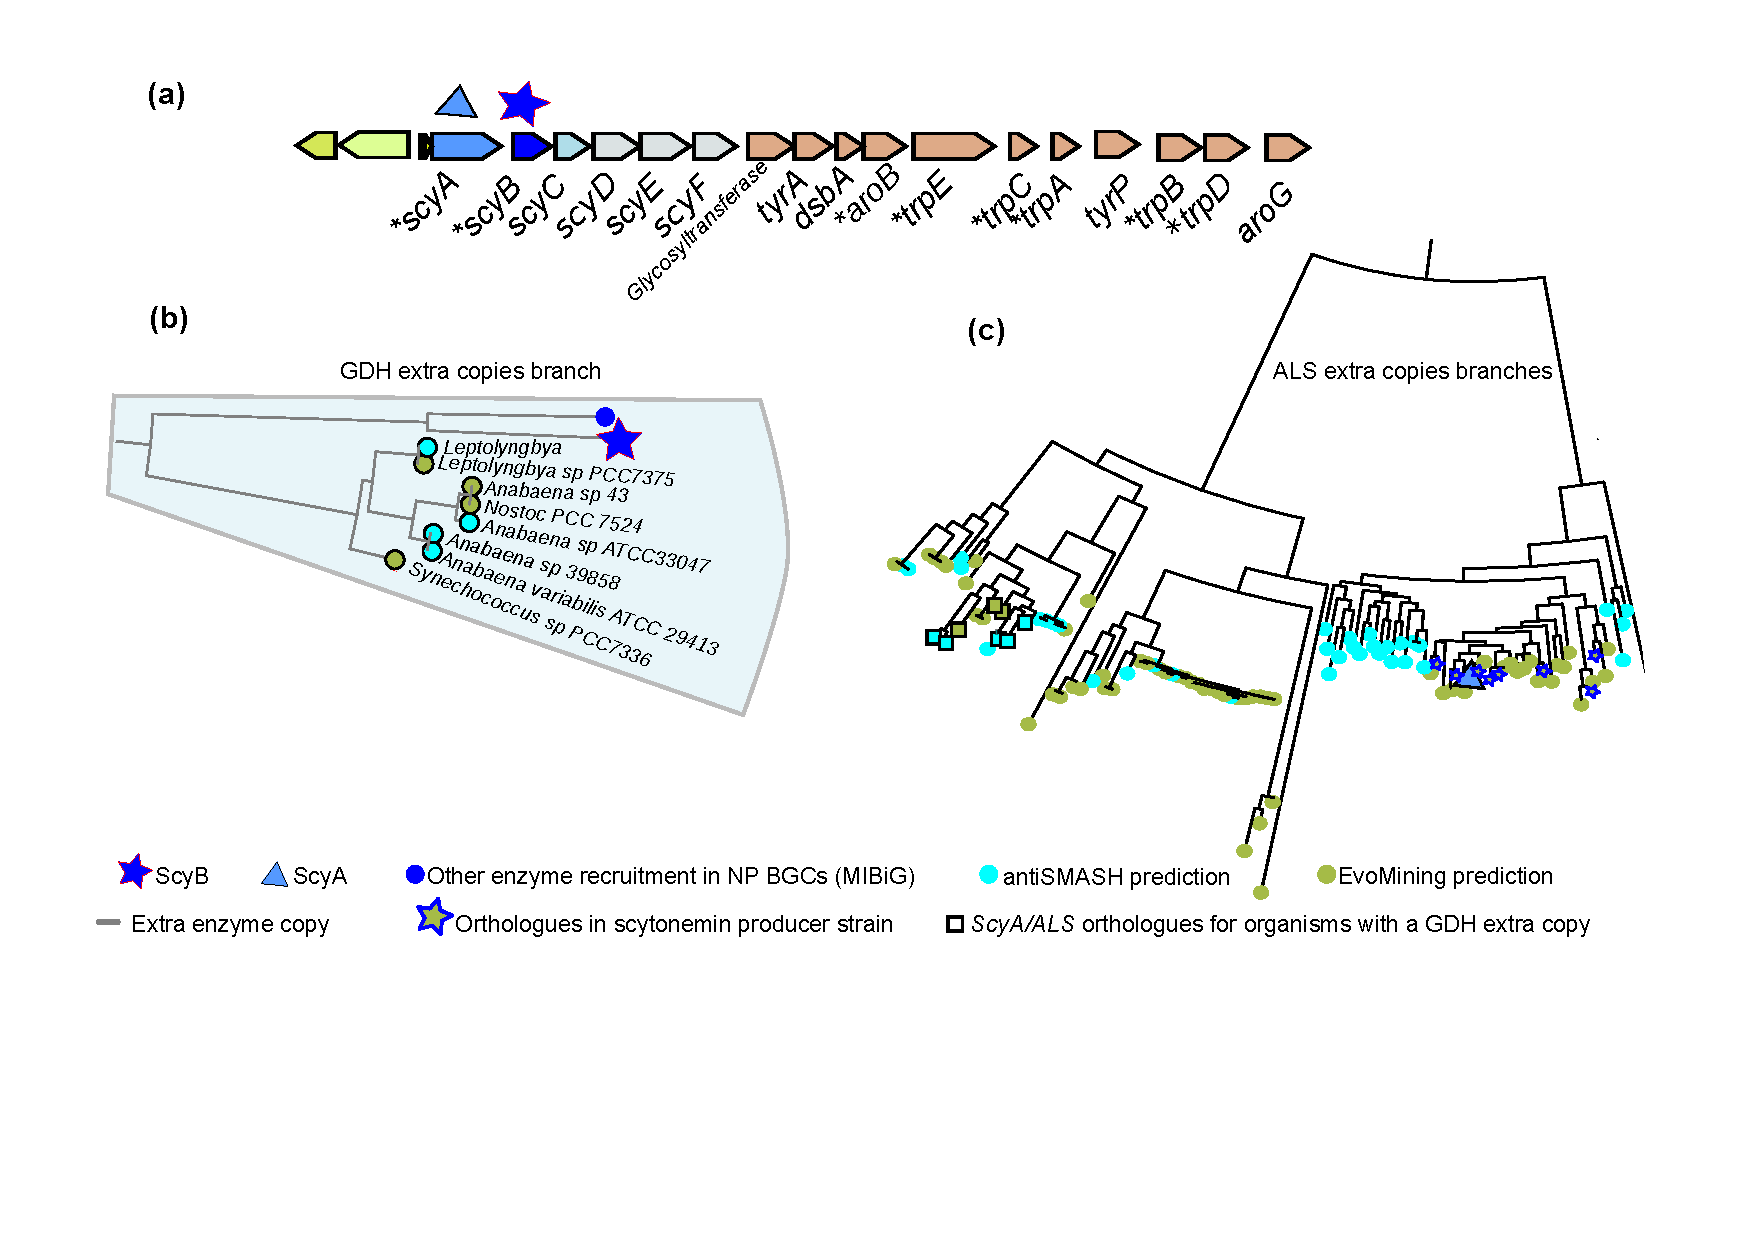
\includegraphics[angle = 0,scale = .6]{chapter2/FigurasPaper/Figure5.pdf}
  \caption[Escitonemina es un reclutamiento en las ramas divergentes de las familias GDH y ALS]{\footnotesize{Reclutamientos de GDH y ALS por el cluster biosintético de escitonemina. (a) El BGC de  escitonemina de $Nostoc punctiforme$ se compone de genes reguladores (verde), genes que participan en la biosíntesis de escitonemina (azul) y de genes dedicados al suministro de precursores (marrón). Se encontró que ocho familias enzimáticas del BGC de escitonemina tienen su origen dentro de las 42 familias enzimáticas conservadas. Estas ocho familias comunes están marcadas con asteriscos. (b) Acercamiento de la rama de expansión de Cyanobacteria GDH cerca de ScyB. Inesperadamente, muchos de los productores conocidos de escitonemina no se encuentran en esta rama. (c) Acercamiento de la rama ScyA, que muestra las expansiones de ALS correcta y exclusivamente marcadas por EvoMining como un destino en el metabolismo especializado. Los productores de escitonemina conocidos están marcados con estrellas. Los cuadrados indican expansiones dedicadas al metabolismo especializado ubicado en la vecindad genómica de las expansiones de GDH que coinciden con la rama ScyB. Los árboles de EvoMining de TrpA, TrpB, TrpC, TrpD, TrpE y AroB de Cyanobacteria están disponibles en Microreact.}}
  \label{fig:Scytonemin}
  \end{figure}
  
  \subsection{GDH y ALS en el cluster escitonemina ejemplifican como
  familias pertenecientes a un mismo BGC pueden tener distintos patrones
  de
  expansión.}\label{gdh-y-als-en-el-cluster-escitonemina-ejemplifican-como-familias-pertenecientes-a-un-mismo-bgc-pueden-tener-distintos-patrones-de-expansion.}
  
  La enzima GDH, se encuentra presente en muchos linajes debido tanto a su
  origen ancestral como a la transferencia horizontal
  {[}\protect\hyperlink{ref-andersson_evolution_2003}{126}{]}
  \autoref{fig:GDHJunto}. GDH cataliza la reacción reversible de
  desaminación oxidativa de glutamato en \(\alpha\)-cetoglutarato y
  amonio. De acuerdo al uso de cofactores, la GDH puede dividirse en tres
  clases, la primera usa NAD+ y es nombrada como GDH(NAD+). La segunda
  clase utiliza NADP+ y es conocida como GDH(NADP+). La tercera clase
  utiliza ambos cofactores NAD+ y NADP+; por lo que se le conoce como
  GDH(NAD+ y
  NADP+){[}\protect\hyperlink{ref-engel_glutamate_2014}{117}{]}.
  
  Aunque existen otras clasificaciones de la diversidad de enzimas GDH
  esta fue seleccionada porque se relaciona con la historia evolutiva de
  la enzima. GDH(NAD+) es utilizada para la oxidación del glutamato
  mientras que GDH(NADP+) para fijar amonio, algunas enzimas de Archaea
  funcionan bien con ambos cofactores, es decir tienen promiscuidad de
  cofactores{[}\protect\hyperlink{ref-engel_glutamate_2014}{117}{]}. La
  especificidad por NAD+ o NADP+ probablemente emergió en repetidas
  ocasiones, una evidencia a favor de esta hipótesis es que se ha mostrado
  que algunas mutaciones pueden revertir la
  especificidad{[}\protect\hyperlink{ref-lilley_partial_1991}{127}{]}.
  Esto sugiere que en los cofactores análogamente al caso de promiscuidad
  por sustrato, la similitud de secuencia no siempre es suficiente para
  evidenciar la especificidad. En ocasiones la divergencia o cercanía
  filogenética de los organismos productores de la enzima es una
  información adicional a la similitud de secuencia, esta consideración es
  importante al analizar enzimas en linajes muy divergentes.
  
  La familia GDH muestra expansiones aunque no muy abundantes en
  \href{https://microreact.org/project/r1IhjVm6X?tt=cr}{Actinobacteria}
  \autoref{fig:GenomicLinajes} panel (a) ,y en
  \href{https://microreact.org/project/HyjYUN7pQ?tt=cr}{Cyanobacteria}
  \autoref{fig:GenomicLinajes} panel(b). Las expansiones están
  prácticamente ausentes en
  \href{https://microreact.org/project/HyjYUN7pQ?tt=cr}{\emph{Pseudomonas}}
  \autoref{fig:GenomicLinajes} panel (c). En contraste, un número
  significativo de expansiones es encontrado en
  \href{https://microreact.org/project/ByUcvNmaX?tt=cr}{Archaea}
  \autoref{fig:GenomicLinajes} panel(d) . El árbol de EvoMining de la
  familia GDH en Archaea fue enraizado con la secuencia semilla de
  \emph{Sulfolobus}, que fue predicha por RAST como una enzima dual en el
  uso de cofactores
  NAD(P)+{[}\protect\hyperlink{ref-consalvi_glutamate_1991}{128}{]}. En
  Archaea las tres clases de GDH alternan en las ramas del
  \href{https://microreact.org/project/ByUcvNmaX?tt=cr}{árbol}
  \autoref{fig:GDHFactor}.
  
  Muchas de las secuencias clasificadas como de metabolismo conservado se
  concentran volviendo rojas las ramas basales del árbol. Se observa otro
  clado más grande y diverso compuesto casi exclusivamente por enzimas
  específicas para
  NAD(P){[}\protect\hyperlink{ref-ferrer_nadp-glutamate_1996}{129}{]},
  incluyendo muchas predicciones de antiSMASH, y sólo dos marcadas como
  metabolismo conservado. Estas dos marcas pueden deberse a la pérdida
  real de una enzima de metabolismo central en las ramas centrales o bien
  a huecos debidos a la calidad del ensamblado y la secuenciación de los
  genomas. La anotación funcional de estos ortólogos de GDH apunta hacia
  reclutamientos en el metabolismo especializado. Estos reclutamientos
  fueron identificados en organismos de los genera \emph{Haladaptatus},
  \emph{Haloterrigena} , \emph{Natrialba} , \emph{Natrinema} ,
  \emph{Natrialbaceae} y \emph{Natronococcus}. Los genes se encuentran un
  contexto de posible síntesis de terpenos. Este contexto incluye enzimas
  relacionadas al geranil pirofosfato, un precursor de todos los terpenos
  y terpenoides{[}\protect\hyperlink{ref-tholl_terpene_2006}{130}{]}. Este
  árbol tiene también casos de divergencia reciente. Hay una pequeña rama
  indistinguible en la figura pero explorable en la plataforma microreact
  donde los parálogos aparecen junto a las secuencias de metabolismo
  central. Finalmente a pesar de la divergencia las últimas ramas
  corresponden a enzimas de metabolismo conservado, es decir son las
  copias más parecidas en esos organismos a las semillas provistas en la
  Enzyme DB \autoref{fig:GenomicLinajes} panel(d).
  
  En contraste con la amplia expansión de GDH relacionada a las
  adaptaciones metabólicas en Archaea, el árbol de Cianobacteria tiene
  copias extra sólo en el \(4.5\%\) de sus genomas (
  \autoref{fig:GenomicLinajes} panel(b) , \autoref{fig:DataTabla42}). En
  esta rama expandida se encontraron cuatro predicciones de antiSMASH y
  cuatro predicciones de EvoMining en la rama que contiene a ScyB el
  homólogo de GDH que fue reclutado por el BGC escitonemina. ScyB es pues
  parte de la síntesis de escitonemina, un pigmento amarillo producido por
  muchas Cyanobacterias como protección contra la radiación UV-A
  solar{[}\protect\hyperlink{ref-balskus_genetic_2010}{131}{]}.
  \emph{Nostoc punctiforme} PCC 73102 es el organismo productor de
  escitonemina cuyo BGC fue caracterizado y anotado en MIBiG. EvoMining
  sólo unas pocas secuencias GDH copias extra de especies de \emph{Nostoc}
  aún cuando se conoce que homólogos de \emph{scyB} pueden encontrarse en
  estos genomas. Esta observación puede deberse a la gran divergencia de
  secuencia entre copias de metabolismo central y de metabolismo
  especializado en estos organismos.
  
  En la vecindad genómica de algunas expansiones de GDH se observó la
  secuencia de ALS, un gen identificado en la literatura como homólogo de
  \emph{scyA}. además, en los BGC conocidos de escitonemina se observó que
  \emph{scyB} se conserva cerca del gen \emph{scyA}
  \autoref{fig:Scytonemin} panel (a). \emph{scyA} es homólogo de la
  subunidad larga de ALS. Esta familia tiene un número promedio de copias
  de \(1.87\%\) en la base de datos Genome DB de Cyanobacteria. La media
  es de hecho de \(2.1\) copias en organismos que contienen al menos una
  copia ALS, pero la moda del número de copias es 1. Estos datos indican
  que muchos organismos tienen más de dos copias de ALS lo que puede
  correlacionar con que esta familia es más dispersa alrededor de la moda.
  
  Al generar el
  \href{https://microreact.org/project/B11HkUtdm?tt=cr.}{árbol de
  EvoMining de ALS en Cyanobacteria}, se observó que \emph{scyA} es un
  reclutamiento que se localiza en una rama repleta de secuencias de ALS
  provenientes de \emph{Nostoc spp.}, que fueron etiquetadas como
  predicciones de EvoMining \autoref{fig:Scytonemin} (c). Estas
  predicciones incluyen más de veinte organismos conocidos como
  productores de escitonemina
  {[}\protect\hyperlink{ref-balskus_investigating_2008}{115}{]}. Además,
  ramas cercanas muestran secuencias de ALS que son predicciones de
  antiSMASH, reforzando la sugerencia de que esta sección del árbol se
  dedica al metabolismo especializado. Una última rama contiene a los
  mismos organismos encontrados en el árbol de EvoMining de la familia
  GDH. Estos organismos son mostrados en el zoom de la rama de \emph{scyB}
  \autoref{fig:Scytonemin} panel(b).
  
  \begin{figure}[h!tbp]
  \centering
  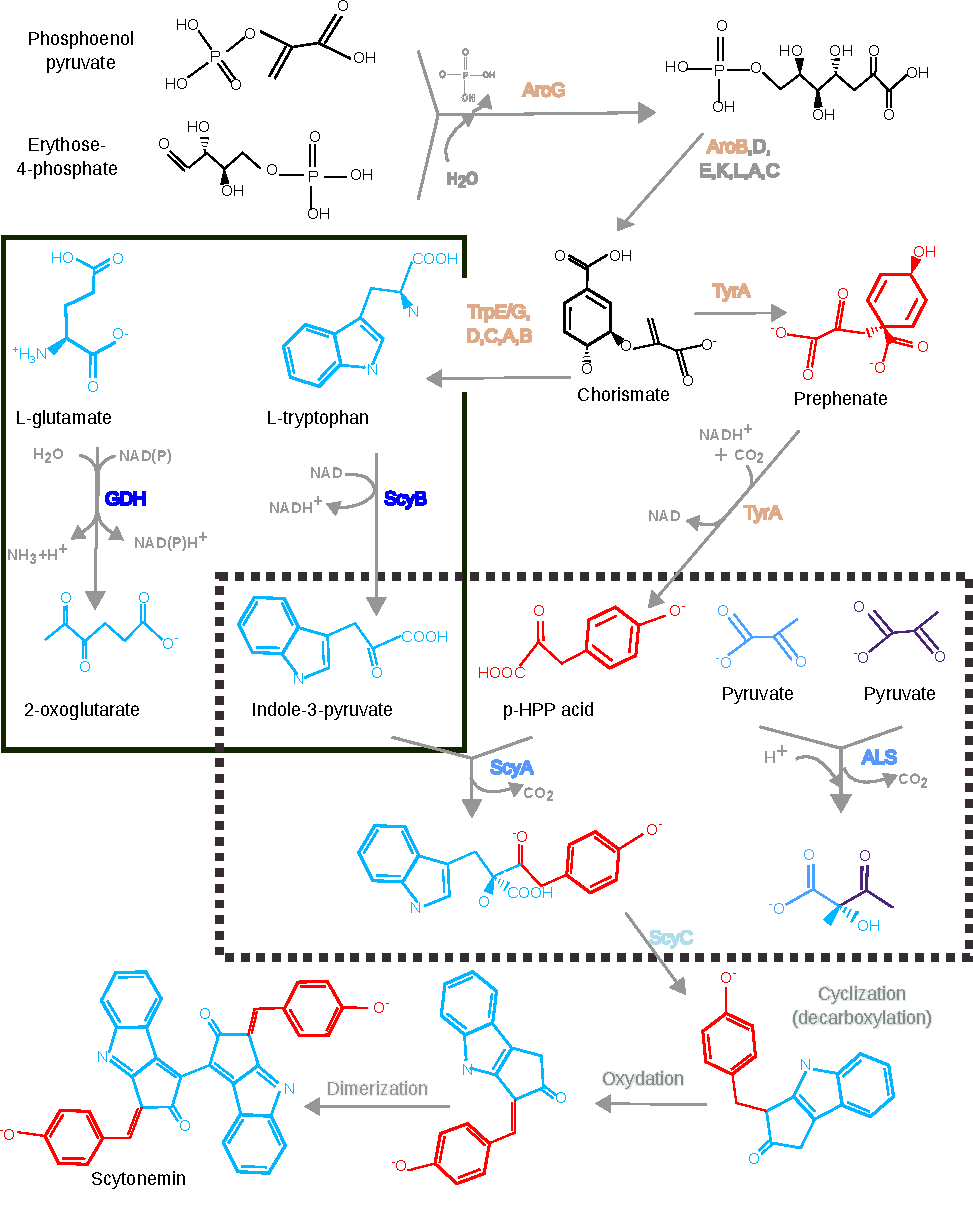
\includegraphics[angle = 0,scale = .8]{chapter2/FigurasPaper/Figure6.pdf}
  \caption[Origen metabólico y destino de GDH / ScyA y ALS / ScyB en la biosíntesis de escitonemina]{\footnotesize{Origen metabólico y destino de GDH / ScyA y ALS / ScyB en la biosíntesis de escitonemina. AroG y AroB participan en la síntesis de corismato, un intermediario que se transforma en los precursores que conducen a sustratos de ScyA, es decir, l-triptófano y prefenato. La reacción catalizada por ScyB que convierte el triptófano en indol-3-piruvato es similar a la conversión de l-glutamato en 2-oxoglutarato, catalizada por GDH (cuadrado con un contorno sólido). ScyA cataliza la descarboxilación de indol-3-piruvato y ácido p-hidroxi-fenil-pirúvico (p-HPP) para formar un dipéptido que sirve como un precursor de escitonemina. Esta reacción es análoga a la descarboxilación de dos piruvatos por la enzima ALS original (rectángulo con un contorno de puntos). ScyC realiza una ciclación seguida de pasos de oxidación y dimerización que concluyen con la ruta de scytonemin. Las enzimas del BGC de escitonemina dedicadas a la síntesis de precursores están coloreadas en marrón y las enzimas biosintéticas en azul.}}
  \label{fig:Ruta}
  \end{figure}
  
  Esta observación sugiere co-diversificación, vía un evento de expansión
  reclutamiento de ScyA y ScyB a partir de su origen en ALS y GDH,
  respectivamente. Los perfiles de expansión de estas familias difieren ya
  que a diferencia de la muy poblada rama de \emph{scyA} en el árbol de
  ALS, la similitud entre homólogos de la FE de GDH y homólogos de ScyB no
  fue suficiente para reconstruir una rama de \emph{scyB} con todas las
  expansiones sugeridas por la ocurrencia del cluster de escitonemina.
  Estas observaciones son una lección a usar EvoMining como herramienta de
  minería genómica, que enzimas cercanas pueden co-diversificarse en
  ocasiones formando parte de un mismo BGC pero a la vez estar sujetas a
  distintas restricciones evolutivas.
  
  \subsection{El cluster de escitonemina es una familia de clusters cuyas
  variantes en los genes accesorios muestran promiscuidad de
  producto.}\label{el-cluster-de-escitonemina-es-una-familia-de-clusters-cuyas-variantes-en-los-genes-accesorios-muestran-promiscuidad-de-producto.}
  
  Definimos \emph{cluster promiscuo} como una familia de BGC homólogos
  cuyos miembros sintetizan distintos productos naturales con la misma
  estructura base pero con algunas modificaciones que son específicas de
  cada organismo incluyendo aquellos BGC que en un mismo organismo pueden
  producir varias moléculas muy similares. Un cluster puede ser promiscuo
  ya sea por la promiscuidad de alguna de sus enzimas o por la diversidad
  en los genes accesorios particulares a cada organismo. En oposición
  tenemos los clusters u operones del metabolismo central, donde la
  selección ya ha actuado siempre obtener el mismo producto, por ejemplo
  algún aminoácido en particular. Como veremos más adelante el BGC de
  escitonemina presenta diversidad de productos.
  
  El \emph{cluster} de la escitonemina reportado en MIBiG y mostrado en la
  figura \autoref{fig:Scytonemin} panel (a) y en \autoref{fig:Ruta}
  comprende 18 genes
  {[}\protect\hyperlink{ref-soule_comparative_2009}{116}{]}. Además de
  genes reguladores, este BGC incluye a los genes genes biosintéticos
  \emph{scyABC}, los genes conservados con función desconocida
  \emph{scyDEF} y los proveedores de precursores: \emph{tyrA},
  \emph{dsbA}, \emph{aroB}, \emph{trpE/G}, \emph{trpC}, \emph{trpA},
  \emph{tyrP}, \emph{trpB}, \emph{trpD}, \emph{aroG}. Las familias
  enzimáticas TrpABCDEG y AroB son parte de las rutas de los aminoácidos
  aromáticos y del ácido shikímico, parecen haber sido reclutadas para
  proveer de los precursores L-triptofano y prefrenato, que son necesarios
  para la síntesis de escitonemina. En oposición a las enzimas del operón
  de triptofano y a AroB que siguen realizando su función de metabolismo
  conservado aún como parte de una ruta de metabolismo especializado están
  ScyA y ScyB. Estas dos familias también tienen un origen en el
  metabolismo conservado, ya se ha explicado que tienen su origen en las
  familias ALS y GDH, pero en este caso sí ha cambiado la especificidad
  por sustrato al momento de la incorporación al metabolismo especializado
  \autoref{fig:Ruta}. ALS une dos piruvatos, transformándolos en
  S-2-acetolactato
  {[}\protect\hyperlink{ref-liu_acetohydroxyacid_2016}{118}{]}, mientras
  que ScyB cataliza la unión de indol-3-piruvato con ácido p-hidroxi-fenil
  pirúvico. De forma análoga, GDH convierte L-glutamato en 2-oxoglutarato
  {[}\protect\hyperlink{ref-engel_glutamate_2014}{117}{]}, mientras que
  ScyA cataliza una desaminación oxidativa de triptofano. El producto de
  estas dos enzimas actuando secuencialmente e un dipéptido, el cual es
  ciclado por ScyC. La ruta metabólica culmina con una serie de
  oxidaciones y dimerizaciones hasta llegar al producto escitonemina, aún
  no es claro como se llevan a cabo estos últimos
  pasos{[}\protect\hyperlink{ref-balskus_investigating_2008}{115}{]}.
  
  \begin{figure}[h!tbp]
  \centering
  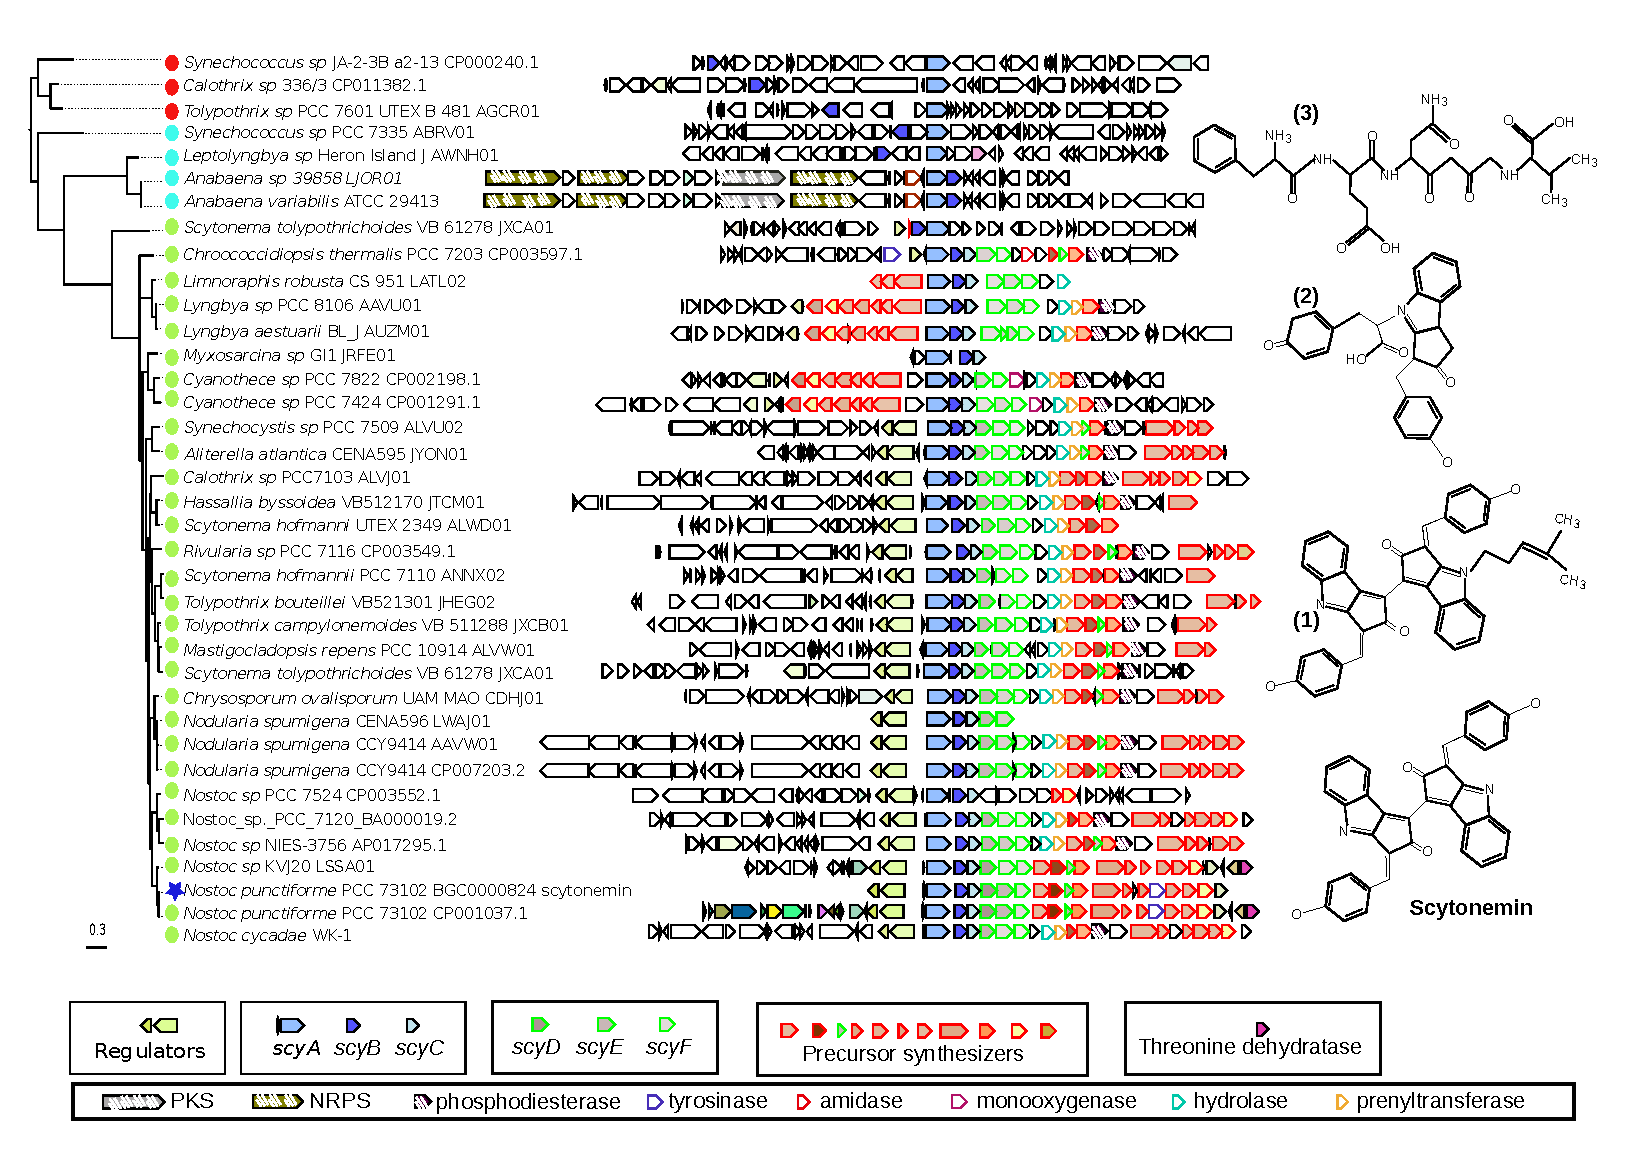
\includegraphics[angle = 90,scale = .8]{chapter2/FigurasPaper/Figure7.pdf}
  \caption[El cluster de scytonemina produce distintos metabolitos]{\footnotesize{El análisis filogenómico de scyA y sycB mostró una diversidad química en torno a la scytonemin BGC. Las proximidades genómicas que contienen tanto scyA como scyB en Cyanobacterias se muestran junto a una reconstrucción filogenética utilizando las secuencias de proteínas de estos dos genes.}}
  \label{fig:CorasonScytonemina}
  \end{figure}
  
  Además de GDH y ALS el BGC de escitonemina tiene seis familias que son
  parte de las 42 FEs analizadas aquí, es decir 8 de los genes que
  participan en la síntesis de escitonemina tienen un origen en
  metabolismo conservado y fueron reclutados en el cluster de escitonemina
  ( \autoref{fig:ExpansionPatterns}, \autoref{fig:Scytonemin}. De estas
  familias, seis de los siete árboles de EvoMining contienen copias extras
  identificadas como predicciones de EvoMining, debido a que en su rama de
  expansión se encuentra el correspondiente gen de escitonemina del
  cluster reportado en MIBiG. Los reclutamientos incluyen AroB y todos los
  genes de la ruta del L-triptofano excepto \emph{trpF}. Estos árboles
  pueden ser consultados interactivamente, los links de microreact están
  anotados en la \autoref{tab:Microreact}.
  
  \begin{figure}[h!tbp]
  \centering
  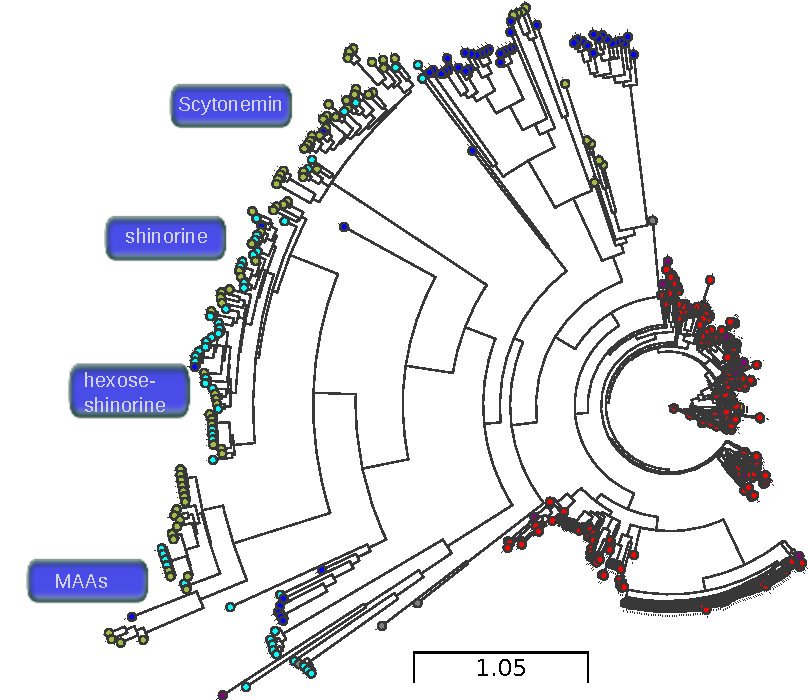
\includegraphics[angle = 0,scale = .9]{chapter2/AroB.pdf}
  \caption[AroB en Cianobacteria]{\footnotesize{Árbol de EvoMining de AroB. El número promedio de copias de esta familia es 1.3, la moda es uno con 29.5 porciento del total de los genomas superando este umbral. Estas características se reflejan en tres ramas llenas de copias adicionales marcadas ya sea como predicciones de antiSMASH o como predicciones de EvoMining. La primera rama de abajo hacia arriba tiene los compuestos MAA como reclutamientos. La segunda rama fue reclutada para la síntesis de shinorine y la tercera rama para la de escitonemina. Estos tres productos naturales MAAs, shinorine y escitonemina son protectores solares. En contraste a las familias del operón de triptofano, AroB no tiene Welwitindolinone, Ambiguine o fischerindoline como reclutamientos}}
  \label{fig:AroB}
  \end{figure}
  
  Los árboles de EvoMining de estas familias incluyen ramas marcadas por
  reclutamientos que son enzimas que forman parte de las rutas de síntesis
  de otros pigmentos protectores solares. Entre ellos la shinorina y los
  aminoácidos de tipo mycosporina (MAAs)\autoref{fig:AroB}
  {[}\protect\hyperlink{ref-balskus_genetic_2010}{131}{]}. Entre los
  reclutamientos también están otros no relacionados a la protección
  solar, como la welwitindolinona
  {[}\protect\hyperlink{ref-hillwig_identification_2014}{132}{]}, la
  ambiguina
  {[}\protect\hyperlink{ref-li_hapalindole_ambiguine_2015}{133}{]} y la
  fischerindolina {[}\protect\hyperlink{ref-li_decoding_2017}{134}{]}.
  Estos resultados ilustran como EvoMining puede complementar a antiSMASH
  mediante la identificación de secuencias que pertenecen de BGC no
  tradicionales.
  
  \begin{longtable}[]{@{}cc@{}}
  \caption{Links de Microreact de árboles relacionados a escitonemina
  \label{tab:Microreact}}\tabularnewline
  \toprule
  Enzima & Familia\tabularnewline
  \midrule
  \endfirsthead
  \toprule
  Enzima & Familia\tabularnewline
  \midrule
  \endhead
  TrpA &
  \url{https://microreact.org/project/SyZMprKum?tt=cr}\tabularnewline
  TrpB &
  \url{https://microreact.org/project/H1jW0rFdX?tt=cr}\tabularnewline
  TrpC &
  \url{https://microreact.org/project/rkN1THFum?tt=cr}\tabularnewline
  TrpE/G &
  \url{https://microreact.org/project/rkv20SFOm?tt=cr}\tabularnewline
  TrpD &
  \url{https://microreact.org/project/H1UuQE0qm?tt=cr}\tabularnewline
  AroB &
  \url{https://microreact.org/project/SkT1Wp_dm?tt=cr}\tabularnewline
  GDH &
  \url{https://microreact.org/project/HyjYUN7pQ?tt=cr}\tabularnewline
  ALS &
  \url{https://microreact.org/project/B11HkUtdm?tt=cr}\tabularnewline
  \bottomrule
  \end{longtable}
  
  Para investigar la coocurrencia de ScyA y ScyB, que son necesarias
  juntas para producir escitonemina, reconstruimos su historia evolutiva
  conjunta. Para ello se obtuvieron las secuencias de lo genomas donde
  ambas tenían presencia, se concatenaron sus secuencias y se realizó una
  filogenia con ellas. Las variantes de la vecindad genómica del BGC de
  escitonemina fueron visualizadas mediante el uso de CORASON
  {[}\protect\hyperlink{ref-navarro-munoz_computational_2018}{110}{]}. En
  el siguiente capítulo será explicado con más detalle este software de
  visualización y organización de vecindades genómicas. Los análisis
  filogenómicos resultaron en 34 Cyanobacterias con diversidad química en
  el BGC de escitonemina. Es decir en conclusión escitonemina es un
  ejemplo de cluster promiscuo, ya que parece haber un \emph{core
  conservado}, pero diversidad en enzimas accesorias y por tanto en sus
  productos finales.
  
  Se pudieron predecir cinco estructuras putativas que son variantes de
  escitonemina y correlacionan con episodios de pérdida y ganancia de
  genes en este locus \autoref{fig:CorasonScytonemina}. En esta figura la
  clasificación de EvoMining para la familia ALS se muestra en un círculo
  acorde con los colores de EvoMining. Al \emph{core} de genes
  \emph{scyABCD} se incorporan genes que realizan ornamentos como
  hidrolasas, prenil-transferasas , fosfodiesterasas y monooxigenasas ,
  para formar congéneres de escitonemina como los compuestos 1 y 2. La
  pérdida de los genes \emph{scyDEF} y la aparición de otras enzimas como
  la tyrosinasa y o la amidasa pueden derivar en la síntesis de los
  compuestos 3 y 4. Además encontramos que homólogos de \emph{scyA} y
  \emph{scyB} son parte de otro BGC que contiene un híbrido NRPS-PKS.
  Siguiendo las reglas biosintéticas de estas enzimas se propuso el
  compuesto 5. La diversidad química sugerida en estas predicciones sólo
  puede ser validada mediante trabajo experimental, sin embargo si existen
  variantes reportadas de la molécula de escitonemina
  {[}\protect\hyperlink{ref-grant_scytonemin-imine_2013}{135}{]}. Las
  variantes producidas por la dinámica evolutiva del metabolismo
  especializado fueron sugeridas mediante el sólo uso de ScyA y ScyB como
  semillas de búsqueda. Estos resultados sugieren el poder predictivo de
  EvoMining para explorar espacios metabólicos típicamente ignorados por
  métodos de búsqueda tradicionales de BGC que no consideran la evolución
  dentro de sus algoritmos de minería genómica.
  
  \section{EvoMining aplicado a TauD, enzima común de los BGC Rimosamide y
  Detoxin sugieren otra clase de clusters con promiscuidad de
  producto.}\label{evomining-aplicado-a-taud-enzima-comun-de-los-bgc-rimosamide-y-detoxin-sugieren-otra-clase-de-clusters-con-promiscuidad-de-producto.}
  
  Además del ejemplo de las familias del BGC de escitonemina ampliamente
  discutido en este capítulo, y de las 42 familias de metabolismo
  conservado apliqué EvoMining para estudiar las expansiones de otras
  familias enzimáticas. Una de ellas es TauD una enzima del \emph{shell
  genome} de Actinobacteria que cuya contraparte homóloga en
  Enterobacteria forma parte del operón de \emph{E. coli} metabolismo de
  taurina. En Actinobacteria una copia de \emph{tauD} pertenece a este
  operón que está parcialmente conservado, mientras que otras copias, cuyo
  destino metabólico nos muestra EvoMining aparecen en una rama marcada
  por reclutamientos de MIBiG, \autoref{fig:tauD}. EvoMining también
  encuentra expansiones de esta familia en \emph{Pseudomonas} donde además
  el contexto genómico de la copia secundaria se conserva cerca de una
  PKS, sugiriendo la pertenencia de \emph{tauD} a BGC de productos
  naturales. En Actinobacteria \emph{tauD} es parte de 15 BGCs
  \autoref{tab:tauD}, entre ellos los \emph{clusters} que producen los
  metabolitos rimosamide y detoxin. Estos metabolitos comparten un
  \emph{core} molecular y difieren en ornamentaciones. Esta observación y
  el hecho de que estos BGC comparten más genes además de la rimosamide,
  nos pueden sugerir que los BGC de rimosamide y detoxin, también pueden
  considerarse como parte de una sola clase de BGCs que presentan
  promiscuidad de producto. El estudio de las variantes de
  rimosamide-detoxin BGC será objeto del siguiente capítulo donde
  cambiaremos de estudiar las variaciones a nivel secuencia de enzimas a
  estudiar variantes de clusters biosintéticos.
  
  \begin{figure}[h!tbp]
  \centering
  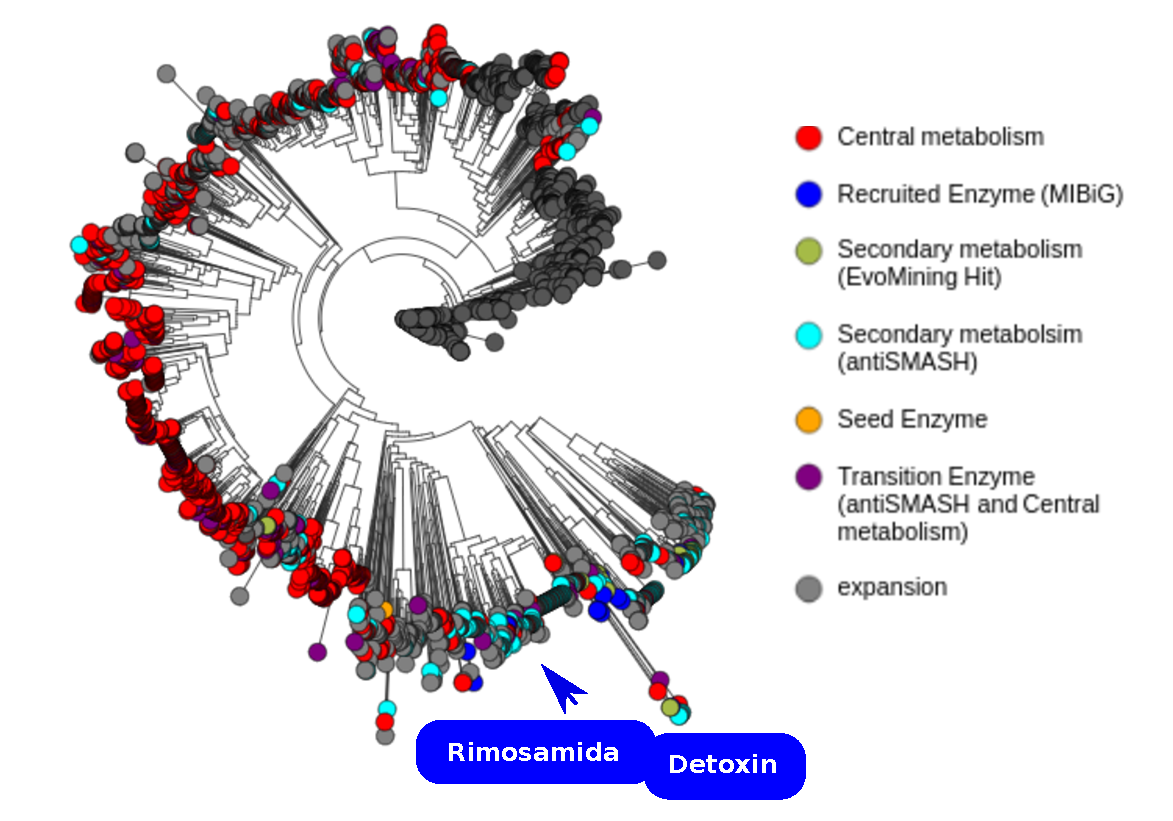
\includegraphics[angle = 0,scale = 0.68]{chapter2/tauD.pdf}
  \caption[Árbol de EvoMining de TauD en Actinobacteria muestra que esta enzima fue reclutada por una familia de BGCs ]{\footnotesize{Análisis de EvoMining de las expansiones de la famila TauD. En Actinobacteria existe una rama dedicada al metabolismo especializado. Dentro de esta rama hay copias extra en géneros como $Streptomyces$, $Rhodococcus$, $Frankia$ y $Amycolatopsis$ . Esta figura muestra un clado dentro de las expansiones de la familia que contiene quince  homólogos de $tauD$ que pertenecen a clusters biosintéticos experimentalmente caracterizados y depositados en MIBiG, incluyendo los de detoxin y rimosamidas. La variedad de BGC mostrada en este clado abre la posibilidad de encontrar variantes moleculares de estas familias.}}
  \label{fig:tauD}
  \end{figure}
  
  \begin{longtable}[]{@{}llll@{}}
  \caption{Homólogos de \emph{tauD} en BGC reportados en
  MIBiG.\label{tab:tauD}}\tabularnewline
  \toprule
  \begin{minipage}[b]{0.19\columnwidth}\raggedright\strut
  MIBiG BGC\strut
  \end{minipage} & \begin{minipage}[b]{0.20\columnwidth}\raggedright\strut
  Compuesto\strut
  \end{minipage} & \begin{minipage}[b]{0.15\columnwidth}\raggedright\strut
  Clase\strut
  \end{minipage} & \begin{minipage}[b]{0.34\columnwidth}\raggedright\strut
  Organismo productor\strut
  \end{minipage}\tabularnewline
  \midrule
  \endfirsthead
  \toprule
  \begin{minipage}[b]{0.19\columnwidth}\raggedright\strut
  MIBiG BGC\strut
  \end{minipage} & \begin{minipage}[b]{0.20\columnwidth}\raggedright\strut
  Compuesto\strut
  \end{minipage} & \begin{minipage}[b]{0.15\columnwidth}\raggedright\strut
  Clase\strut
  \end{minipage} & \begin{minipage}[b]{0.34\columnwidth}\raggedright\strut
  Organismo productor\strut
  \end{minipage}\tabularnewline
  \midrule
  \endhead
  \begin{minipage}[t]{0.19\columnwidth}\raggedright\strut
  653\_ADO85576\strut
  \end{minipage} & \begin{minipage}[t]{0.20\columnwidth}\raggedright\strut
  pentalenolactone\strut
  \end{minipage} & \begin{minipage}[t]{0.15\columnwidth}\raggedright\strut
  Terpene\strut
  \end{minipage} & \begin{minipage}[t]{0.34\columnwidth}\raggedright\strut
  \emph{Streptomyces arenae}\strut
  \end{minipage}\tabularnewline
  \begin{minipage}[t]{0.19\columnwidth}\raggedright\strut
  678\_BAC70706\strut
  \end{minipage} & \begin{minipage}[t]{0.20\columnwidth}\raggedright\strut
  pentalenolactone\strut
  \end{minipage} & \begin{minipage}[t]{0.15\columnwidth}\raggedright\strut
  Terpene\strut
  \end{minipage} & \begin{minipage}[t]{0.34\columnwidth}\raggedright\strut
  \emph{Streptomyces avermitilis} NBRC 14893\strut
  \end{minipage}\tabularnewline
  \begin{minipage}[t]{0.19\columnwidth}\raggedright\strut
  163\_ACR50790\strut
  \end{minipage} & \begin{minipage}[t]{0.20\columnwidth}\raggedright\strut
  tetronasin\strut
  \end{minipage} & \begin{minipage}[t]{0.15\columnwidth}\raggedright\strut
  Polyketide\strut
  \end{minipage} & \begin{minipage}[t]{0.34\columnwidth}\raggedright\strut
  \emph{Streptomyces longisporoflavus}\strut
  \end{minipage}\tabularnewline
  \begin{minipage}[t]{0.19\columnwidth}\raggedright\strut
  961\_ABC36162\strut
  \end{minipage} & \begin{minipage}[t]{0.20\columnwidth}\raggedright\strut
  bactobolin\strut
  \end{minipage} & \begin{minipage}[t]{0.15\columnwidth}\raggedright\strut
  NRP-Polyketide\strut
  \end{minipage} & \begin{minipage}[t]{0.34\columnwidth}\raggedright\strut
  \emph{Burkholderia thailandensis} E264\strut
  \end{minipage}\tabularnewline
  \begin{minipage}[t]{0.19\columnwidth}\raggedright\strut
  287\_AAG05698\strut
  \end{minipage} & \begin{minipage}[t]{0.20\columnwidth}\raggedright\strut
  2-amino-4-methoxy- trans-3- butenoic acid\strut
  \end{minipage} & \begin{minipage}[t]{0.15\columnwidth}\raggedright\strut
  NRP\strut
  \end{minipage} & \begin{minipage}[t]{0.34\columnwidth}\raggedright\strut
  \emph{Pseudomonas aeruginosa} PAO1\strut
  \end{minipage}\tabularnewline
  \begin{minipage}[t]{0.19\columnwidth}\raggedright\strut
  846\_ctg1\_orf9\strut
  \end{minipage} & \begin{minipage}[t]{0.20\columnwidth}\raggedright\strut
  tabtoxin\strut
  \end{minipage} & \begin{minipage}[t]{0.15\columnwidth}\raggedright\strut
  Other\strut
  \end{minipage} & \begin{minipage}[t]{0.34\columnwidth}\raggedright\strut
  \emph{Pseudomonas syringae}\strut
  \end{minipage}\tabularnewline
  \begin{minipage}[t]{0.19\columnwidth}\raggedright\strut
  1183\_AGC09526\strut
  \end{minipage} & \begin{minipage}[t]{0.20\columnwidth}\raggedright\strut
  lobophorin\strut
  \end{minipage} & \begin{minipage}[t]{0.15\columnwidth}\raggedright\strut
  Polyketide\strut
  \end{minipage} & \begin{minipage}[t]{0.34\columnwidth}\raggedright\strut
  \emph{Streptomyces} sp. FXJ7.023\strut
  \end{minipage}\tabularnewline
  \begin{minipage}[t]{0.19\columnwidth}\raggedright\strut
  1156\_ADD83004\strut
  \end{minipage} & \begin{minipage}[t]{0.20\columnwidth}\raggedright\strut
  platencin\strut
  \end{minipage} & \begin{minipage}[t]{0.15\columnwidth}\raggedright\strut
  Terpene\strut
  \end{minipage} & \begin{minipage}[t]{0.34\columnwidth}\raggedright\strut
  \emph{Streptomyces platensis}\strut
  \end{minipage}\tabularnewline
  \begin{minipage}[t]{0.19\columnwidth}\raggedright\strut
  1140\_ACO31277\strut
  \end{minipage} & \begin{minipage}[t]{0.20\columnwidth}\raggedright\strut
  platensimycin- platencin\strut
  \end{minipage} & \begin{minipage}[t]{0.15\columnwidth}\raggedright\strut
  Terpene\strut
  \end{minipage} & \begin{minipage}[t]{0.34\columnwidth}\raggedright\strut
  \emph{Streptomyces platensis}\strut
  \end{minipage}\tabularnewline
  \begin{minipage}[t]{0.19\columnwidth}\raggedright\strut
  1140\_ACO31282\strut
  \end{minipage} & \begin{minipage}[t]{0.20\columnwidth}\raggedright\strut
  platensimycin- platencin\strut
  \end{minipage} & \begin{minipage}[t]{0.15\columnwidth}\raggedright\strut
  Terpene\strut
  \end{minipage} & \begin{minipage}[t]{0.34\columnwidth}\raggedright\strut
  \emph{Streptomyces platensis}\strut
  \end{minipage}\tabularnewline
  \begin{minipage}[t]{0.19\columnwidth}\raggedright\strut
  715\_ABW87795\strut
  \end{minipage} & \begin{minipage}[t]{0.20\columnwidth}\raggedright\strut
  spectinomycin\strut
  \end{minipage} & \begin{minipage}[t]{0.15\columnwidth}\raggedright\strut
  Saccharide\strut
  \end{minipage} & \begin{minipage}[t]{0.34\columnwidth}\raggedright\strut
  \emph{Streptomyces spectabilis}\strut
  \end{minipage}\tabularnewline
  \begin{minipage}[t]{0.19\columnwidth}\raggedright\strut
  1205\_KGO40485\strut
  \end{minipage} & \begin{minipage}[t]{0.20\columnwidth}\raggedright\strut
  communesin\strut
  \end{minipage} & \begin{minipage}[t]{0.15\columnwidth}\raggedright\strut
  Polyketide\strut
  \end{minipage} & \begin{minipage}[t]{0.34\columnwidth}\raggedright\strut
  \emph{Penicillium expansum}\strut
  \end{minipage}\tabularnewline
  \begin{minipage}[t]{0.19\columnwidth}\raggedright\strut
  1205\_KGO40482\strut
  \end{minipage} & \begin{minipage}[t]{0.20\columnwidth}\raggedright\strut
  communesin\strut
  \end{minipage} & \begin{minipage}[t]{0.15\columnwidth}\raggedright\strut
  Polyketide\strut
  \end{minipage} & \begin{minipage}[t]{0.34\columnwidth}\raggedright\strut
  \emph{Penicillium expansum}\strut
  \end{minipage}\tabularnewline
  \begin{minipage}[t]{0.19\columnwidth}\raggedright\strut
  1183\_AGC09525\strut
  \end{minipage} & \begin{minipage}[t]{0.20\columnwidth}\raggedright\strut
  lobophorin\strut
  \end{minipage} & \begin{minipage}[t]{0.15\columnwidth}\raggedright\strut
  Polyketide\strut
  \end{minipage} & \begin{minipage}[t]{0.34\columnwidth}\raggedright\strut
  \emph{Streptomyces} sp. FXJ7.023\strut
  \end{minipage}\tabularnewline
  \begin{minipage}[t]{0.19\columnwidth}\raggedright\strut
  654\_ABB69741\strut
  \end{minipage} & \begin{minipage}[t]{0.20\columnwidth}\raggedright\strut
  phenalinolactone\strut
  \end{minipage} & \begin{minipage}[t]{0.15\columnwidth}\raggedright\strut
  Saccharide-Terpene\strut
  \end{minipage} & \begin{minipage}[t]{0.34\columnwidth}\raggedright\strut
  \emph{Streptomyces} sp. Tu6071\strut
  \end{minipage}\tabularnewline
  \begin{minipage}[t]{0.19\columnwidth}\raggedright\strut
  1070\_CAN89617\strut
  \end{minipage} & \begin{minipage}[t]{0.20\columnwidth}\raggedright\strut
  kirromycin\strut
  \end{minipage} & \begin{minipage}[t]{0.15\columnwidth}\raggedright\strut
  NRP - Polyketide\strut
  \end{minipage} & \begin{minipage}[t]{0.34\columnwidth}\raggedright\strut
  \emph{Streptomyces collinus} Tu 365\strut
  \end{minipage}\tabularnewline
  \bottomrule
  \end{longtable}
  
  \section{Consideraciones finales sobre el uso de
  EvoMining}\label{consideraciones-finales-sobre-el-uso-de-evomining}
  
  EvoMining fue desarrollado como una herramienta de minería genómica
  descargable que puede ser aplicada a bases de datos de secuencias de
  metabolismo conservado (Enzyme DB) provenientes de familias enzimáticas
  de distintos phyla. Nuestros análisis llevaron a la conclusión de que
  los patrones de expansión reclutamiento dependen tanto de la familia
  enzimática como del linaje genómico en el que se analiza. Una
  consideración importante al usar EvoMining es que el tamaño de genoma
  correlaciona con el número de copias extra de familias expandidas.
  Aunque el tamaño de genoma es importante, también encontramos
  excepciones donde EvoMining pudo predecir enzimas de BGC no
  tradicionales en genomas relativamente pequeños, sugiriendo que hacen
  falta más análisis para estudiar esta relación. En este sentido, optamos
  por comparar linajes genómicos que no solo son altamente divergentes y,
  en algunos casos, poco conocidos con respecto a la biosíntesis de NP,
  sino también desproporcionados en cuanto a su resolución taxonómica y
  distancias. Por lo tanto, es posible que estos factores hayan impuesto
  un sesgo al establecer relaciones entre el tamaño del genoma, la tasa de
  expansión de genes y la diversidad metabólica.
  
  Es interesante observar que las familias más expandidas según los
  análisis de prueba de concepto anteriores de EvoMining
  {[}\protect\hyperlink{ref-cruz-morales_phylogenomic_2016}{61}{]} fueron
  asparagina sintasa, 2-dehidro-3-deoxifosfoheptanoato aldolasa y
  3-fosfosquimato-1-carboxivinil transferasa, que son las que llevaron al
  descubrimiento de enzimas biosintéticas de arsenolípidos. Cabe destacar
  que ninguna de estas enzimas formaba parte de los 42 FE analizados en el
  presente documento, lo que refuerza la idea de que no solo las enzimas
  conservadas, sino también las enzimas del \emph{shell} con copias
  adicionales, pueden servir como semillas para el descubrimiento de
  nuevos BGC. Después de observar que la familia de la GDH tiene numerosas
  expansiones en Archaea pero no en otros taxones, proporcionamos un
  ejemplo de un reclutamiento de una enzima metabólica central por un BGC
  en Cianobacteria, donde no hay tantas expansiones, lo que sugiere que
  las predicciones en Arhea deben ser exploradas experimentalmente. Estas
  observaciones enfatizan la naturaleza predictiva de EvoMining.
  
  En este punto conviene enfatizar cómo fue clave el papel de MIBiG
  {[}\protect\hyperlink{ref-medema_minimum_2015}{112}{]} para esta versión
  de EvoMining ya que permite incrementar consistentemente y sin esfuerzo
  de curación manual a los BGC reportados por investigadores de todo el
  mundo. La versión previa de EvoMining no incluía por ejemplo ningún BGC
  de Cianobacteria o de Archaea. Gracias a esta actualización que la nueva
  versión de EvoMining pudo identificar correctamente secuencias de genes
  del BGC de la escitonemina. Sin la presencia de la señal de los BGC de
  Cianobacteria en MIBiG estas hojas habrían sido catalogadas como de
  destino metabólico desconocido.
  
  En este capítulo se describió el funcionamiento de EvoMining y sus
  aplicaciones como una herramienta de minería genómica que permite
  relacionar la historia evolutiva de familias enzimáticas con su función.
  Específicamente, lo empleamos para señalar familias de genes con
  expansiones que sugieren la presencia de elementos con promiscuidad.
  También, EvoMining fue utilizado para ubicar a los homólogos de familias
  expandidas que probablemente forman parte de BGC. Estos últimos
  seguramente producen nuevos productos naturales, razón por la cual,
  abordaremos el estudio de la conservación de estos BGC a partir de estas
  enzimas en el siguiente capítulo. Se mostró también que el metabolismo
  se puede expandir a partir de genes de metabolismo conservado
  considerando tanto el metabolismo \emph{shell}, como el metabolismo
  \emph{core}. Se ilustró con el ejemplo de escitonemina que en un BGC se
  encuentran genes provenientes de la expansión de distintas familias de
  enzimas, que una misma expansión puede ser utilizada para producir
  distintos análogos con estructuras similares y que los patrones de
  expansión son específicos de cada familia y linaje. Queda por explorar
  los patrones de neofuncionalización de forma exhaustiva con todas las
  familias del \emph{shell genome} así como el determinar de los BGCs
  conocidos en MIBiG qué familias del metabolismo conservado fueron las
  que les dieron origen. En el siguiente capítulo retomaremos el ejemplo
  de \emph{tauD} para describir el descubrimiento de 3 nuevos BGC cuyo
  producto natural fue sido demostrado por colaboradores.
  
  \chapter{Desarrollo de CORASON como herramienta para organizar clusters
  biosintéticos y otras vecindades genómicas
  conservadas.}\label{desarrollo-de-corason-como-herramienta-para-organizar-clusters-biosinteticos-y-otras-vecindades-genomicas-conservadas.}
  
  En este capítulo presento CORASON, \emph{CORe Analysis of Syntenic
  Orthologs to prioritize Natural products biosynthetic gene clusters},
  una herramienta para explorar la diversidad en el contenido de los
  \emph{Clusters} de Genes Biosintéticos (BGC por sus siglas en inglés)
  así como su distribución en un linaje proporcionado por el usuario.
  CORASON es una herramienta en línea de comandos para organizar
  filogenéticamente la variación de una familia de clusters, Figura
  \autoref{fig:Corason-pipe}. Ya que sabemos que hay variantes de BGC que
  producen productos naturales similares dentro de los linajes genómicos.
  Otros métodos de minado de genomas han acelerado el descubrimiento de
  nuevos BGC. Casi cada nueva bacteria que es secuenciada aporta alguna
  novedad al pangenoma bacteriano conocido. Una fracción de estos genes
  descubiertos formará parte de variantes de BGC previamente conocidos
  aportando diversidad a las familias de clusters biosintéticos. La
  diversidad genética que existe en las familias de BGCs está relacionada
  con cambios moleculares, incluso pequeñas variantes en un metabolito
  pueden ocasionar diferencias en su función biológica por lo que es de
  interés identificar análogos de productos naturales tanto como entender
  su evolución. Se diseñó CORASON que identifica el \emph{core} génico de
  un BGC y genera una visualización de las variantes de la familia
  organizadas filogenéticamente.
  
  \begin{figure}[h!tbp]
  \centering
  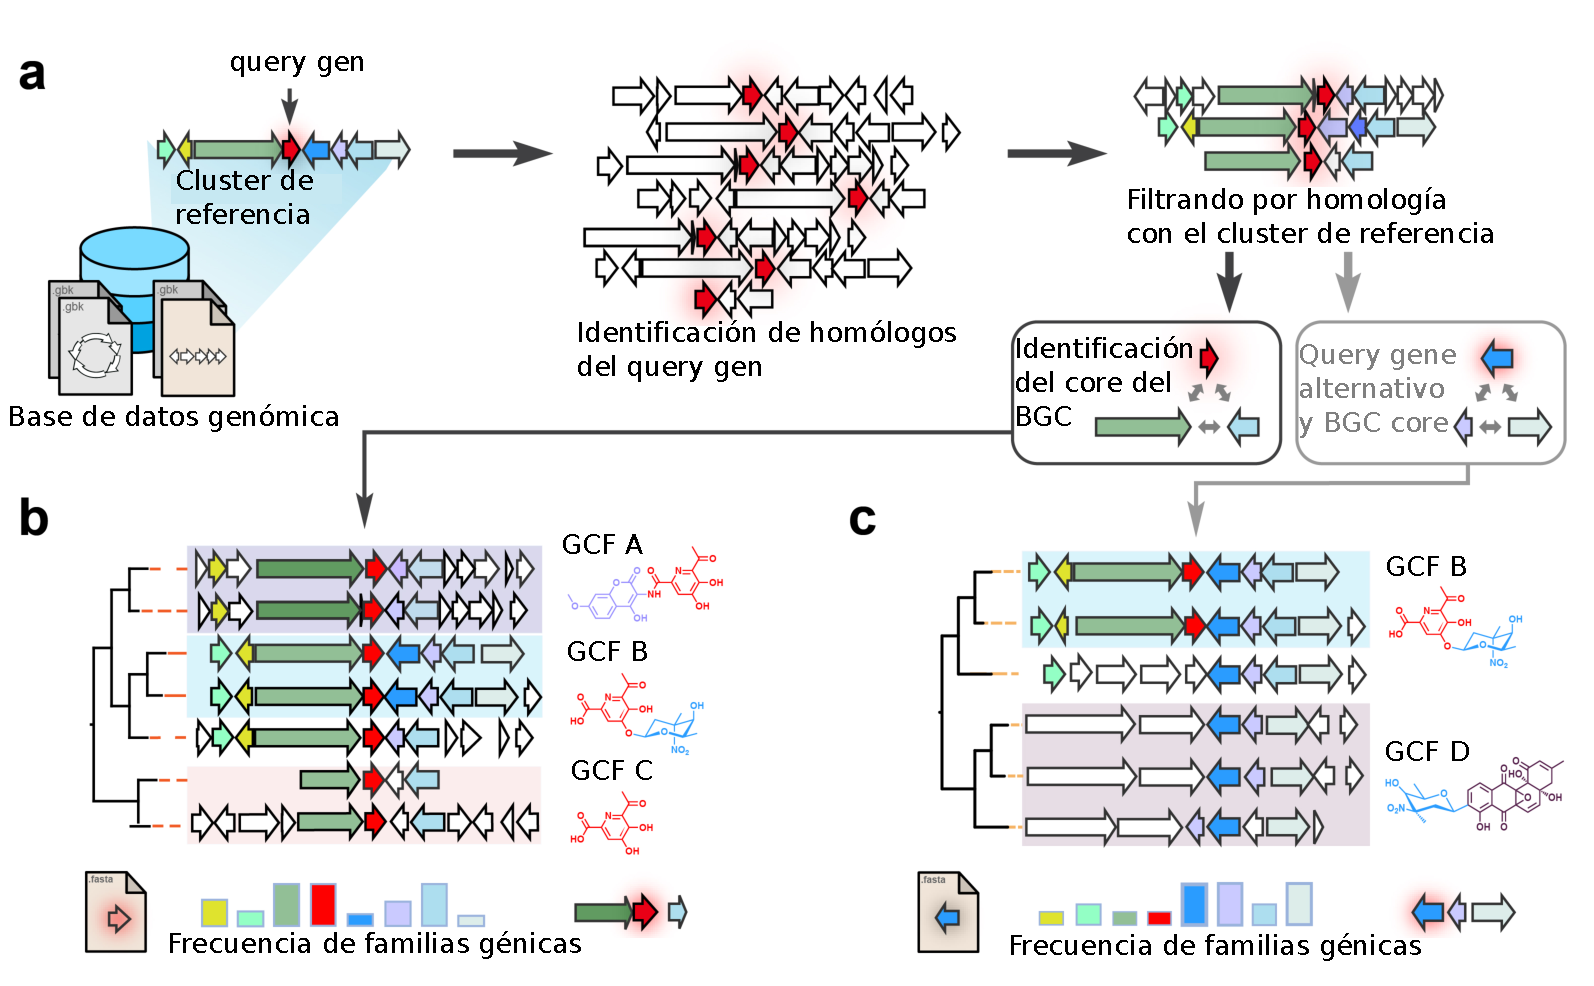
\includegraphics[angle = 0,scale = .6]{chapter3/Corason-pipe.pdf}
  \caption[La herramienta corason localiza familias de clusters biosintéticos en un linaje genómico partiendo de un cluster y un gen de referencia.]{\footnotesize{La herramienta corason localiza familias de clusters biosintéticos en un linaje genómico partiendo de un cluster y un gen de referencia. Todos los contextos genómicos que contengan ese gen y algún otro gen del cluster de referencia serán encontrados en el linaje seleccionado por el usuario. CORASON identifica el $core$ génico de la familia. La información del $core$ se utiliza para organizar filogenéticamente todos los miembros de la familia del BGC, es decir todas las variantes del BGC serán organizadas. El core génico está relacionado con el $core$ de la molécula, la parte variable del BGC codifica enzimas accesorias que producen ornamentos. Al cambiar de gen de referencia CORASON permite explorar otras familias de BGC que contengan las mismas modificaciones. Los resultados se presentan en una visualización que permite al mismo tiempo apreciar variación a nivel de presencia-ausencia de genes entre miembros de una familia de BGCs, como también apreciar variación a nivel de secuencia a través de un gradiente de color entre genes conservados entre una variante y el BGC de referencia.}}
  \label{fig:Corason-pipe}
  \end{figure}
  
  \section{Algoritmo y características de
  CORASON}\label{algoritmo-y-caracteristicas-de-corason}
  
  La herramienta corason, como se muestra en la \autoref{fig:Corason-pipe}
  localiza familias de BGC en un linaje genómico partiendo de un
  \emph{cluster} y un gen de referencia. Para ello el usuario debe proveer
  una base de datos de genomas (Genome DB) de un linaje definido con las
  mismas características y precauciones descritas para EvoMining el
  capítulo anterior. También debe poner como entrada un BGC y un gen de
  referencia que sea parte de ese BGC. El algoritmo de CORASON busca los
  homólogos de ese gen en cada genoma de la base de datos y luego también
  detecta a los otros genes del BGC de referencia si es que se encuentran
  en la vecindad del gen de referencia. Esto lo repite para todas las
  secuencias del linaje seleccionado por el usuario. Posteriormente,
  CORASON identifica el \emph{core} génico de la familia con el algoritmo
  de Orthocore. La información del \emph{core} se utiliza para organizar
  filogenéticamente todos los miembros de la familia del BGC. Ya que el
  \emph{core} génico está relacionado con el \emph{core} de la molécula,
  CORASON permite detectar en la parte variable del BGC a las enzimas
  accesorias que producen ornamentos i.e.~variantes moleculares. Los
  resultados son un árbol en formato Newick junto con una visualización
  que permite al mismo tiempo apreciar variación a nivel de
  presencia-ausencia de genes entre miembros de una familia de BGCs así
  como la divergencia a nivel de secuencia entre genes conservados entre
  una variante y el BGC de referencia, mismo que se distingue con un
  código de color.
  
  CORASON fue diseñado con las siguientes características: (i) Se
  implementa en una interfaz de línea de comando simple. (ii)
  Identificación de todos los homólogos de un gen de referencia en una
  base de datos de genomas. (iii) Identificación del \emph{core} génico
  del BGC. (iv) Reconstrucción filogenética de la familia de BGCs
  utilizando la información del \emph{core}. (v) Salida visual en formato
  SVG, que muestra tanto la anotación funcional de los genes como como la
  distancia respecto a sus ortólogos del \emph{cluster} de referencia.
  
  \section{Las familias de BGC son variantes del BGC de
  referencia.}\label{las-familias-de-bgc-son-variantes-del-bgc-de-referencia.}
  
  Así como existen familias génicas, un gen y todos sus homólogos,
  incluidos parálogos, ortólogos y xenólogos, también existen familias de
  BGCs. Sin embargo no es trivial definir los límites de un BGC porque no
  tiene un codón de inicio y un codón de paro como un gen. En algunas
  ocasiones como en el caso de escitonemina todos los genes del BGC se
  expresan al recibir un estímulo, como los rayos UV en este caso. Otras
  veces en la producción del metabolito participan genes que no son
  necesariamente contiguos, y por ello al cambiar el BGC de organismo y
  realizar expresión heteróloga no se obtiene el mismo metabolito.
  
  Así pues, cuando se habla de un BGC no se debe pensar que este es igual
  en todos los organismos del linaje, es decir que tiene el mismo
  contenido génico. Hay variación tanto a nivel de contenido génico como a
  nivel de secuencia entre los genes ortólogos. Esta variación produce la
  promiscuidad de producto, una familia de BGC produce distintos productos
  a partir de precursores similares. En este trabajo tomamos como BGC de
  referencia a los anotados en MIBiG, que son de los que se tienen
  productos reportados con datos experimentales. Para CORASON consideramos
  como parte de la familia del BGC todas las variantes de BGC que
  contengan al menos dos genes en común, uno de referencia seleccionado
  por el usuario y otro cualquiera pero común con el BGC de referencia.
  
  Como ejemplo de familias de BGC conviene pensar en analogía con los
  operones. Un operón es el conjunto de genes dedicados a la síntesis de
  un mismo proceso que regulan de forma coordinada su propia expresión,
  estos genes suelen ser contiguos y transcribirse simultáneamente desde
  un solo promotor. Ejemplos de estos operones son los que producen los
  aminoácidos histidina y triptófano. Estos ``BGC'' hace millones de años
  fueron posiblemente parte del metabolismo especializado y debido a su
  éxito se fijaron en lo que ahora vemos como BGCs conservados en ciertos
  linajes genómicos. En estos casos las fronteras son claras y la
  variación génica es poca. Aún así existen otros ejemplos donde puede
  constatarse variación en las rutas de síntesis de mecanismos centrales
  de metabolismo procariota. En el caso de histidina y triptófano, como
  hablaremos en el siguiente capítulo, es la variación a nivel de
  secuencia y no tanto a nivel de composición génica la que produce
  diversidad de producto. En oposición a los BGCs u operones de
  metabolismo conservado, están los BGCs del metabolismo especializado,
  así como se encuentran familias con mucha variación génica pueden
  encontrarse otras muy conservadas.
  
  En las siguientes secciones presento cuatro ejemplos que ilustran como
  CORASON puede ser utilizado tanto para priorizar nuevos BGCs como para
  ligar la variación génica de familias de BGCs con diversidad
  estructural. Asimismo se describe cómo este algoritmo es una expansión
  de las habilidades de EvoMining para encontrar enzimas en el proceso de
  diversificación funcional. En resumen, CORASON encuentra familias de
  BGCs, y presenta una rápida visualización de sus variantes. Con esta
  herramienta podemos expandir nuestro conocimiento sobre nuevas variantes
  químicas mediante la genómica comparativa. CORASON está disponible en su
  contenedor de docker en github \url{https://github.com/nselem/corason}.
  
  \section{Aplicaciones de CORASON en Actinobacteria y
  Pseudomonas}\label{aplicaciones-de-corason-en-actinobacteria-y-pseudomonas}
  
  En el capítulo anterior las variantes del BGC escitonemina en
  Cyanobacteria fueron encontradas al aplicar CORASON a dicho linaje. En
  este capítulo presento ejemplos del uso de CORASON para investigar los
  patrones de conservación/variación en familias de BGCs en los linajes
  Actinobacteria y \emph{Pseudomonas}. Primero, las versiones iniciales de
  CORASON fueron usadas junto con cromatografía y espectrometría de masas
  (LC-MS) para estudiar la ecología y evolución de los sideróforos del
  tipo desferroxiaminas en
  Actinobacteria{[}\protect\hyperlink{ref-cruz-morales_actinobacteria_2017}{136}{]}.
  En un segundo ejemplo, CORASON fue utilizado para investigar la
  existencia de variantes en Actinobacteria del cluster productor de
  arsenolípidos que se encuentra en \emph{Streptomyces lividans}.
  Finalmente, un tercer ejemplo es presentado: el de los contextos
  genómicos del metabolismo secundario de \emph{tauD}. Esta enzima
  proviene de una dioxigenasa involucrada en el metabolismo de taurina en
  su papel de enzima del metabolismo conservado. En Actinobacteria
  \emph{tauD} es parte de 15 BGC reportados en MIBiG, aunque en
  \emph{Pseudomonas} no existen BGCs reportados EvoMining predice
  expansiones en este linaje genómico y CORASON predice conservación en
  los contextos genómicos de estas copias extra que guardan cierta
  similitud con variantes de los BGC conocidos en Actinobacteria
  \autoref{fig:PseudomonasTauD} .
  
  \section{Detectamos variantes de sideróforos en Actinobacterias de vida
  libre}\label{detectamos-variantes-de-sideroforos-en-actinobacterias-de-vida-libre}
  
  El hierro es necesario en el metabolismo de muchos seres vivos. Para
  poder utilizarlo las bacterias han desarrollado moléculas captadoras de
  hierro llamadas sideróforos. Un ejemplo de sideróforo es la molécula de
  desferroxiamina sintetizada por los genes \emph{des} en Actinobacteria.
  Usamos CORASON para identificar variantes del cluster biosintético de
  desferroxiamina \autoref{fig:des} Actinobacterias de cuatro ciénegas. En
  particular, encontramos una variante del BGC que se diferencia del
  cluster reportado por la ganancia de un miembro de la familia
  penicilina-amidasa. Al gen que codifica esa función se le llamó
  \emph{desG} y es responsable de la arilación de desferroxiaminas en
  actinomicetos acuáticos
  {[}\protect\hyperlink{ref-cruz-morales_actinobacteria_2017}{136}{]}. Ya
  fue verificado que la variación génica está ligada con la variación
  molecular.
  
  \begin{figure}[h!tbp]
  \centering
  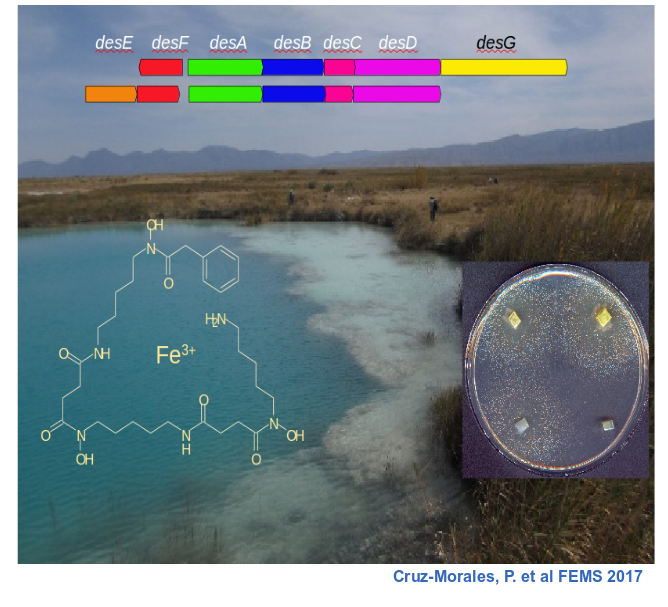
\includegraphics[angle = 0,scale = .4]{chapter3/des.png}
  \caption[EvoMining Algorithm]{\footnotesize{Variantes del cluster biosintético de desferroxiamina fueron identificadas por CORASON en Actinobacterias de cuatro ciénegas. Una variante del BGC de desferroxiamina fue identificada. Esta variante se diferencia del cluster reportado por la ganancia de una penicilin amidasa. A este gen extra se le llamó $desG$.}}
  \label{fig:des}
  \end{figure}
  
  \section{Un BGC de metabolismo de arsénico tiene variantes que conforman
  una familia de
  BGCs}\label{un-bgc-de-metabolismo-de-arsenico-tiene-variantes-que-conforman-una-familia-de-bgcs}
  
  Analizamos los patrones de expansión-reclutamiento de la
  3-fosfoshikimato-1-carboxivinyl transferasa (AroA) en el linaje de
  \emph{Streptomyces} usando EvoMining. Se encontró un cambio de función
  en esta familia tal que en una de las ramas de expansiones se detectó
  específicamente una arsenoenol piruvato sintasa. Estudios de mutagénesis
  y de expresión diferencial génica en presencia de arsénico confirmaron
  que en \emph{Streptomyces coelicolor} y en \emph{Streptomyces lividans}
  esta enzima pertenece a un BGC que sintetiza arsenolípidos
  {[}\protect\hyperlink{ref-cruz-morales_phylogenomic_2016}{61}{]}.
  Mediante curación manual se descubrió por la diversidad en las
  secuencias de aminoácidos que el contexto genómico de AroA en estos
  organismos incluye una enzima PKS localizada a seis genes de distancia.
  AntiSMASH predice los BGCs tipo PKS de estas enzimas pero no incluye en
  ellos a la arsenoenol piruvato sintasa. El valor de EvoMining fue
  descubrir que esta copia extra de AroA estaba dedicada al metabolismo
  especializado y por tanto bien podía tener su propio BGC o dada la
  cercanía con las PKS podía ser parte de estos PKS-BGCs. Nos preguntamos
  si la diversidad de secuencia a nivel de BGC, si se encuentran variantes
  con distintos patrones de presencia/ausencia en los genes que componen
  al BGC de \emph{S coelicolor}. O más aun, quedaba por investigar si el
  BGC tenía cierto grado de conservación o era exclusivo de estos dos
  organismos \emph{S. coelicolor y S. lividans}
  
  El contexto genómico conservado en las expansiones de AroA puede
  apreciarse en la \autoref{fig:Coelicolor}. La arsenoenol piruvato
  sintasa fue descubierta en un árbol de EvoMining como parte de una rama
  de expansiones de AroA en Actinobacteria. El contexto genómico de la
  arsenoenol piruvato sintasa de \emph{S. coelicolor } tiene un \emph{core
  conservado} en Actinobacteria. Este BGC está dedicado a la síntesis de
  metabolitos secundarios de tipo arsenolípidos. Primero se identificaron
  en otras secuencias genómicas contextos que contengan el homólogo de
  AroA y algún otro gen de su vecindad en \emph{S. coelicolor}. A
  continuación, se ordenaron manualmente los contextos obtenidos y se pudo
  identificar al menos cuatro diferentes subclases de BGC. La primera
  clase mostrada en un rectángulo morado no contiene PKS o NRPS, la
  segunda enmarcada en verde contiene una PKS-NRPS híbrida. Los otros dos
  subgrupos solo contienen una PKS, en un caso está río arriba y en otro
  río abajo de AroA. La tercera clase incluye una PKS a la izquierda y a
  más de cinco genes de distancia de la arsenoenol piruvato sintasa;
  finalmente la última clase contiene una PKS a la derecha a sólo un gen
  de distancia de esta enzima. Así, se muestra que existen variantes de un
  BGC que contienen un \emph{core} común, presumiblemente pueden producir
  variantes de arseno compuestos.
  
  \begin{figure}[h!tbp]
  \centering
  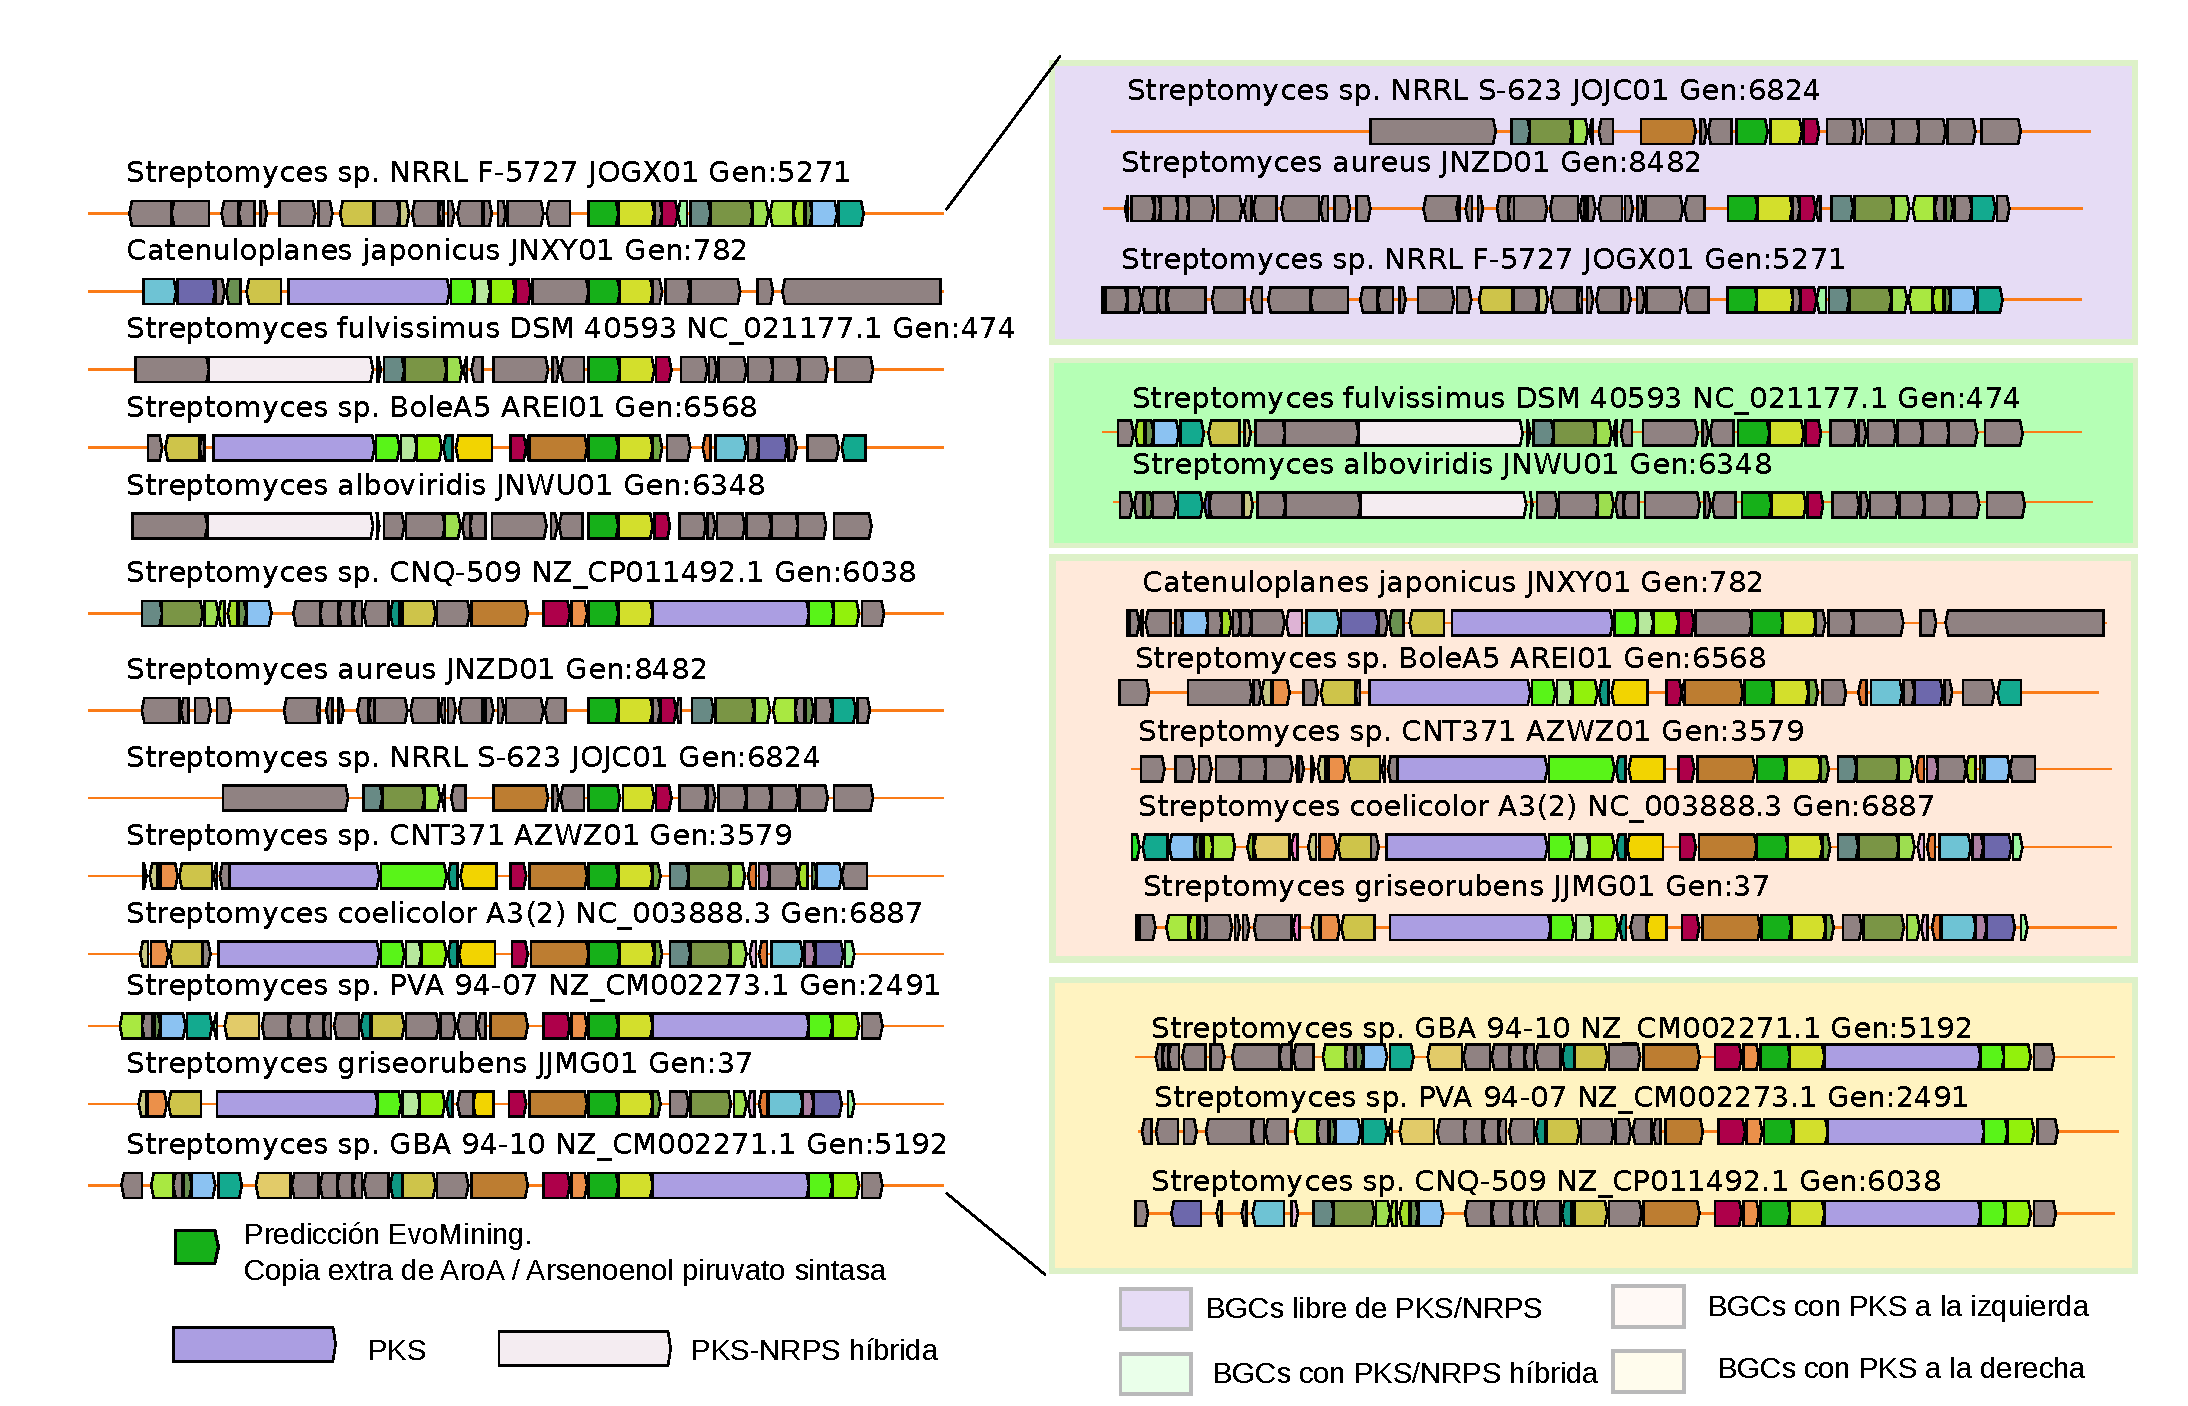
\includegraphics[angle = 0,scale = .4]{chapter3/Coelicolor.pdf}
  \caption[EvoMining Algorithm]{\footnotesize{El contexto genómico conservado en las expansiones de AroA sugiere que es una familia de BGC con promiscuidad de productos. El contexto genómico de la arsenoenol piruvato sintasa de $S.~coelicolor$ tiene un $core~conservado$ en Actinobacteria que produce arsenolípidos. Se identificaron cuatro clases de BGCs. La primera clase en morado no contiene PKS o NRPS, la segunda enmarcada en verde contiene una PKS-NRPS híbrida. La tercera clase incluye una PKS a la izquierda y a más de cinco genes de distancia de la Arsenoenol piruvato sintasa y finalmente la última clase contiene una PKS a la derecha y a sólo un gen de distancia de esta enzima.}}
  \label{fig:Coelicolor}
  \end{figure}
  
  Hasta esta versión de CORASON la visualización realizada para los
  arsenolípidos no incluía ningún tipo de orden y era difícil distinguir
  grupos de BGCs. Por esta razón se pensó que el orden filogenético ya no
  de una enzima sino del \emph{core} del BGC ordenaría las variantes del
  BGC. Este orden mostraría en un continuo la dinámica genómica del BGC
  establecida por los procesos evolutivos. En el caso de los arsenolípidos
  se utilizó Orthocore para la identificación del \emph{core} del BGC. En
  las siguientes versiones de CORASON esta característica fue implementada
  como parte del algoritmo.
  
  \section{Combinamos CORASON y BiG-SCAPE para mejorar la clasificación de
  BGC y logramos predecir dos nuevos compuestos de la familia
  rimosamide-detoxin que fueron caracterizados
  experimentalmente}\label{combinamos-corason-y-big-scape-para-mejorar-la-clasificacion-de-bgc-y-logramos-predecir-dos-nuevos-compuestos-de-la-familia-rimosamide-detoxin-que-fueron-caracterizados-experimentalmente}
  
  BIG-SCAPE es una herramienta bioinformática para clasificar un conjunto
  de BGC en familias de acuerdo al contenido, conservación y distribución
  de sus dominios
  {[}\protect\hyperlink{ref-navarro-munoz_computational_2018}{110}{]}. Un
  dominio es una región conservada de una proteína que evoluciona y
  funciona independientemente del resto de la proteína. La identificación
  de dominios es particularmente importante en los BGC porque las
  modificaciones químicas que catalizan los genes de los BGC
  frecuentemente están codificadas en dominios que pueden o no ser parte
  del mismo gen conservado pero que de cualquier forma repiten la misma
  reacción. Es decir un dominio con la función conservada, puede realizar
  el mismo paso de una ruta biosíntética formando parte de genes que no
  son homólogos. BIG-SCAPE usa la conservación de dominios (no de genes)
  para agrupar BGC en diferentes familias de \emph{clusters}, sin embargo
  no permite una visualización eficiente su evolución. Por ello se utilizó
  una parte del algoritmo de CORASON que al proporcionar un algoritmo para
  ordenar la diversidad dentro de la familia usando el \emph{core} de
  dominios conservados \autoref{fig:CORASONAlgorithm} . Así se consigue
  proponer la filogenia de los BGC y en ocasiones conectar mediante la
  evolución a familias de BGC aparentemente separadas por BiGSCAPE.
  
  \begin{figure}[h!tbp]
  \centering
  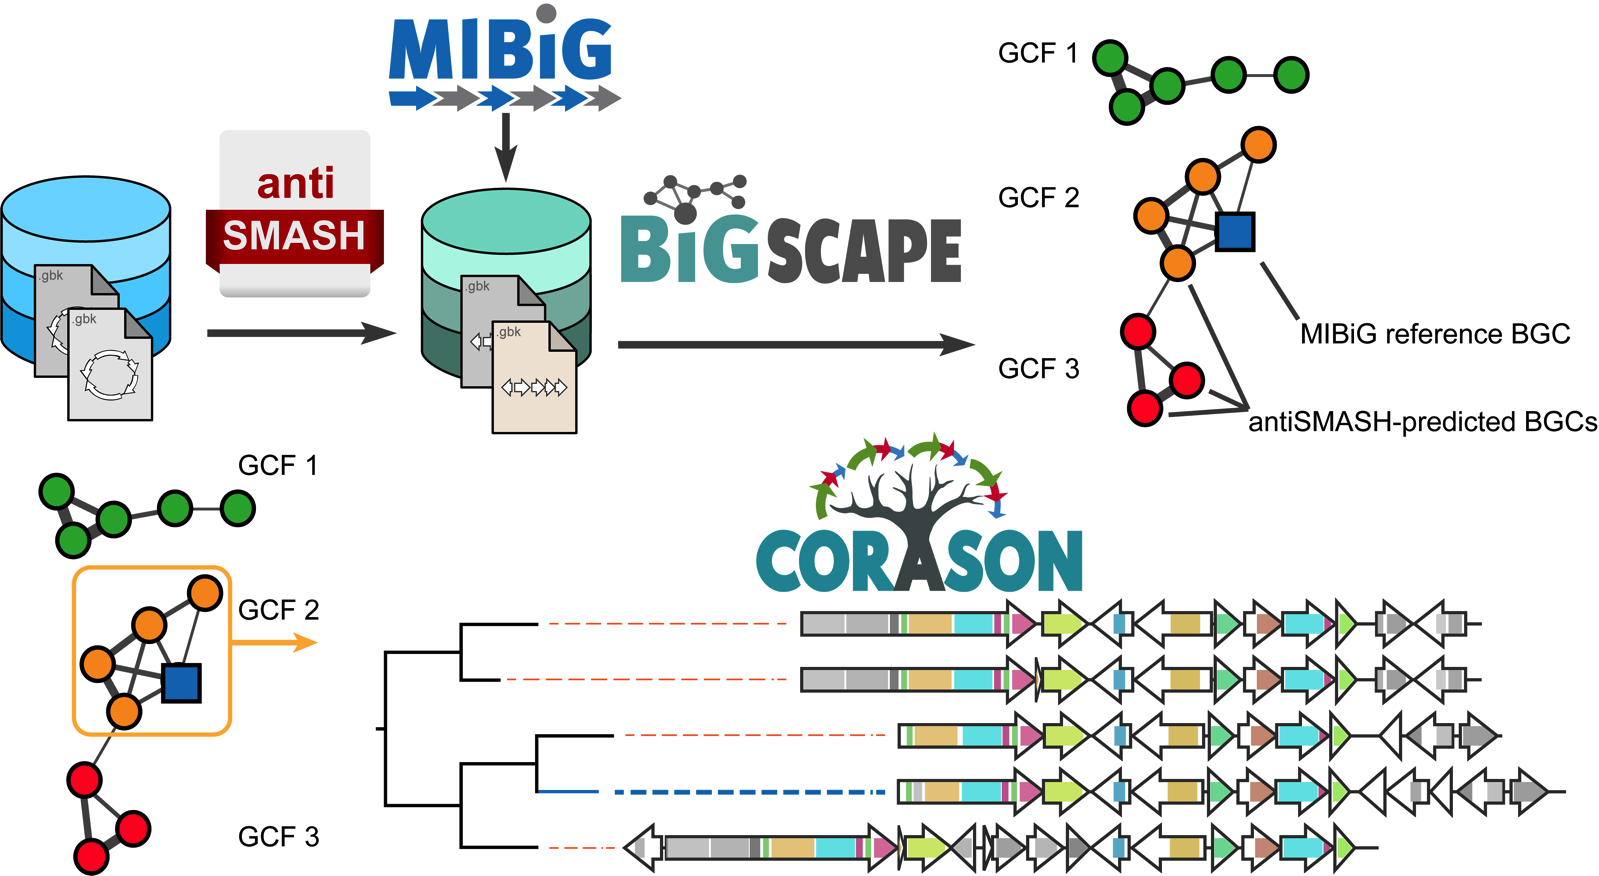
\includegraphics[angle = 0,scale = .3]{chapter3/corason_fig1.png}
  \caption[Algoritmo de CORASON Algorithm]{\footnotesize{CORASON permite ordenar visualizar las familias de genes propuestas por BIG SCAPE. BIG SCAPE toma BGC que pueden provenir de MIBiG, de AntiSMASH y los clasifica en familias (GCF1, GCF2 y GCF3) que comparten dominios conservados. Con corason encontramos el $core$ de dominios para hacer la filogenia de los BGC con ellos y visualizar su evolución }}
  \label{fig:CORASONAlgorithm}
  \end{figure}
  
  \subsection{Identificamos nuevos productos variantes de la familia de
  BGCs Rimosamide - Detoxin en Actinobacteria integrando BiG SCAPE y
  CORASON}\label{identificamos-nuevos-productos-variantes-de-la-familia-de-bgcs-rimosamide---detoxin-en-actinobacteria-integrando-big-scape-y-corason}
  
  Ya que el TauD fue sugerida por un análisis de EvoMining como una
  familia con expansiones reclutadas a productos naturales de distintas
  subfamilias en Actinobacterias, en esta sección utilizamos CORASON y
  BIG-SCAPE para analizar una base de datos de miles de genomas. Con estas
  herramientas se organizó la diversidad biosintética de las familias de
  BGC detoxin y rimosamide
  {[}\protect\hyperlink{ref-mcclure_elucidating_2016}{137}{]}. El análisis
  reveló diversidad tanto en los géneros de los organismos que contienen a
  esta familia, y en la composición génica del BGC. Entre los géneros con
  alguna variante del BGC están \emph{Amycolatopsis}, \emph{Streptomyces}.
  El \emph{core conservado} de los BGCs detoxin y rimosamide está
  compuesto por una NRPS, una NRPS/PKS híbrida, y un homólogo de
  \emph{tauD}. En \emph{E.coli} tauD se encuentra en el operón
  \emph{tauABCD}. La ruta de síntesis de rimosamide difiere de la de
  detoxins porque tiene una NRPS adicional, que codifica para una
  modificación del \emph{core} de molécula detoxin/rimosamide con
  isobutirato y glicina.
  
  El hecho de que el gen \emph{tauD} estuviera presente en todos los
  miembros de la familia \autoref{fig:Rimosamide} captó nuestra atención.
  El TauD pertenece a la super familia de enzimas hidroxilasas
  dependientes de Fe(II)/\(\alpha\)-ketoglutarato. En particular
  \emph{tauD} codifica una taurina dioxigenasa dependiente de
  \(\alpha\)-ketoglutarato involucrada en la asimilación de sulfito por la
  liberación oxigenolítica del aminoácido taurina. Interesantemente, esta
  familia también está presente en linajes como hongos, bacterias y
  plantas. Dichas enzimas catalizan hidroxilaciones, desaturaciones,
  expansiones y formaciones de anillos entre otras transformaciones
  químicas. A la fecha, el rol de TauD en la biosíntesis de los
  metabolitos detoxin y rimosamide aún es desconocido, se ha sugerido que
  es responsable de la oxidación de la prolina observada en algunos
  análogos.
  
  Para identificar variantes de los BGC relacionados a detoxin y
  rimosamide dentro de la rama de metabolismo especializado los 1175 BGC
  que contenían un homólogo de \emph{tauD} se pasaron por un análisis
  combinado de BiG-SCAPE/CORASON. Se uso \emph{tauD} como gen de
  referencia en CORASON ya que es el único gen miembro del `BGC core' que
  está presente en todos los genomas. Es importante notar que el
  \emph{core} del BGC podría contener hasta 3 genes porque la NRPS, y la
  NRPS-PKS híbrida quedan fuera en este ejemplo debido a que algunos
  genomas no están completamente secuenciados y justamente hay huecos a
  los extremos de los contigs que contienen estos BGC. Este es el caso de
  los organismos \emph{Streptomyces humi}, \emph{Streptomyces spectabilis}
  y \emph{Amycolatopsis vancoresmycina}{]}
  
  \begin{figure}[h!tbp]
  \centering
  \includegraphics[angle = 0,scale = .8]{chapter3/figura5.pdf}
  \caption[Rimosamide]{\footnotesize{Visualización de la Familia Expandida de BGC de TauD detectada por CORASON y sus 5 subfamilias de BGC detectadas por BIG SCAPE. A la derecha se muestra la molécula producida por cada subfamilia.}}
  \label{fig:Rimosamide}
  \end{figure}
  
  \subsection{CORASON sugiere que las familias detoxin y rimosamide
  pertenecen a un amplio grupo de familias dedicadas a la síntesis de
  péptidos.}\label{corason-sugiere-que-las-familias-detoxin-y-rimosamide-pertenecen-a-un-amplio-grupo-de-familias-dedicadas-a-la-sintesis-de-peptidos.}
  
  El análisis de CORASON reveló que las familias de los BGC detoxin y
  rimosamide identificados en BiG-SCAPE eran parte de una familia
  expandida de BGC de biosintesis de péptidos que incluía clados
  inexplorados del phylum Actinobacteria \autoref{fig:Rimosamide}. La
  organización filogenética de los BGCs provista por CORASON, reveló
  familias de BGCs que fueron omitidas debido al umbral utilizado por el
  algoritmo de clustering de BiG-SCAPE. Esto debido a la cercanía de genes
  biosintéticos detectados por antiSMASH como suficientemente diferentes
  como para ser clasificados en otras familias.
  
  Hipotetizamos que las detoxins codificadas por los BGCs en los clados
  inexplorados contendrán cierta novedad química relacionada con las
  variaciones genéticas. Afortunadamente, 40 de las 152 cepas
  identificadas como portadoras de un BGC estaban representadas en
  nuestros datos metabolómicos de 363--cepas por LC-MS/MS. Los análisis de
  redes moleculares de estos datos indicaron la presencia de tres detoxin
  conocidas, cuatro rimosamide conocidas y otras 103 variantes de detoxin
  o rimosamide, el basto universo químico sugerido por el análisis
  BiG-SCAPE/CORASON.
  
  \subsection{Aglunos clados selectos del árbol de CORASON que contiene a
  las familias rimosamide/detoxin contienen diversidad génica que
  correlaciona con novedad
  química.}\label{aglunos-clados-selectos-del-arbol-de-corason-que-contiene-a-las-familias-rimosamidedetoxin-contienen-diversidad-genica-que-correlaciona-con-novedad-quimica.}
  
  Tres de los clados que codifican para detoxin BGC fueron identificados
  por BiG-SCAPE dentro del árbol de CORASON capturaron nuestro interés
  (ver las cajas coloreadas de la \autoref{fig:Rimosamide}). En esta
  sección se describe el trabajo experimental realizado por Michael
  Mulloney del grupo de colaboradores de West Chicago, de los tres clados
  y específicamente de los organismos que seleccioné como candidatos a
  presentar diversidad química.
  
  \subsubsection{El clado P450/enoyl agrega una heptanamida al core
  molecular
  detoxin/rimosamide}\label{el-clado-p450enoyl-agrega-una-heptanamida-al-core-molecular-detoxinrimosamide}
  
  El primer clado es el `P450/enoyl clade' contiene genes como el
  citocromo P450 y una enoil-CoA hydratasa/isomerasa dentro de cada uno de
  sus BGC. Este clado está marcado en rojo \autoref{fig:Rimosamide}.
  Análisis de datos por tandem MS de extractos de \emph{Streptomyces} sp.
  NRRL S-325, que se encuentra dentro de este clado, llevó al
  descubrimiento de la detoxin S1. Este nuevo análogo contiene una cadena
  lateral de heptanamide, una estructura única entre las detoxins y
  rimosamides cuya instalación posiblemente depende de la enzima enoyl-CoA
  hydratase/isomerase.
  
  \subsubsection{El superclado spectinomycin/ detoxin-rimosamide produce
  cinco variantes de
  detoxin.}\label{el-superclado-spectinomycin-detoxin-rimosamide-produce-cinco-variantes-de-detoxin.}
  
  El segundo clado de interés,fue nombrado el `supercluster clade'
  (\autoref{fig:Rimosamide}, en verde claro), comprende los BGCs con genes
  de detoxin adyacentes al cluster que produce espectinomycina. El cluster
  de espectinomycina (MIBiG BGC0000715) contiene en su periferia al gen
  \emph{tauD} como se muestra en la línea gris punteada de la
  \autoref{fig:Rimosamide}. La secuencia del cluster de spectinomycin
  depositada en MIBiG es la única secuencia disponible de
  \emph{Streptomyces spectabilis} NRRL 2792. Como no se sabe que tauD
  participe en la síntesis de spectinomycin se hipotetizó que pueden
  existir los genes del cluster de detoxin al lado de los genes del BGC de
  espectinomycina en \emph{S. spectabilis} NRRL 2792. Adquirimos esta cepa
  para determinar si el análisis de CORASON podía ayudar a la predicción
  de detoxin basado solamente en la presencia del gen de referencia pero
  en ausencia completa de la secuencia del BGC de detoxin. El análisis en
  tandem de espectrometría de masas de extracto \emph{S. spectabilis} NRRL
  2792 reveló la presencia de cinco compuestos tipo detoxin.
  
  Los tiempos de retención de iones y los patrones de fragmentación de los
  últimos dos compuestos también fueron observados en extractos de
  \emph{Streptomyces} sp. NRRL B-1347 parte del clado del supercluster.
  Esto confirma la habilidad de CORASON para guiar un descubrimiento
  mediante la utilización de la filogenia a pesar de lo limitado de los
  datos en la cepa NRRL-2792. El análisis de LC-MS de cultivos de
  NRRL-2792 suplementados con isotopos estables etiquetados de amino
  acidos corroboraron las predicciones estructurales basadas en los
  análisis de la cepa cercana \emph{Streptomyces} sp. NRRL B-1347. Aunque
  los datos de MS fueron insuficientes para desenmascarar esta estructura,
  el compuesto 2 fue producido por \emph{S. spectabilis} NRRL 2792 en
  suficiente abundancia para el aislamiento y la elucidación estructural
  por NMR.
  
  \subsubsection{\texorpdfstring{El clado \emph{Amycolatopsis P450}
  produce cinco variantes de
  detoxin.}{El clado Amycolatopsis P450 produce cinco variantes de detoxin.}}\label{el-clado-amycolatopsis-p450-produce-cinco-variantes-de-detoxin.}
  
  El tercer clado que se estudió es al que pertenecen las familias
  rimosamide-detoxin, contiene BGCs casi enteramente provenientes del
  género \emph{Amycolatopsis}. Este clado está marcado en morado en la
  (\autoref{fig:Rimosamide}. Este clado de BGCs también contienen un gen
  P450 único entre los BGCs del árbol, así que fue llamado el clado
  `\emph{Amycolatopsis} /P450 clade'. Aunque no se contaba con datos
  metabolómicos de las cepas del clado de BGC definidos por BiG-SCAPE como
  una \emph{Gen Cluster Family} (GCF), la visualización filogenética de
  CORASON permitió la selección de una cepa de \emph{Amycolatopsis} de la
  que se tenían datos metabolómicos con un BGC muy similar, y que también
  contiene el gen P450 ((\autoref{fig:Rimosamide}, línea gris cerca del
  clado \emph{Amycolatopsis}/P450 ). Los análisis de los datos de tandem
  MS de extracto fermentado de \emph{Amycolatopsis jejuensis} NRRL B-24427
  reveló isómeros de detoxins P1 que contienen tirosina, P2 mostrando
  fenilalanina y una valina hidroxilada, así como la detoxin P3, un
  análogo cercano libre de hidroxilación. Además se consiguió validar la
  asignación de aminoácidos observados en los patrones de fragmentación de
  MS/MS mediante el uso de experimentos de incorporación de isótopos
  estables etiquetados de aminoácidos.
  
  \section{CORASON permitió explorar la promiscuidad de familias de BGCs
  de enzimas divergentes de metabolismo
  central.}\label{corason-permitio-explorar-la-promiscuidad-de-familias-de-bgcs-de-enzimas-divergentes-de-metabolismo-central.}
  
  Nuestros resultados ilustran como BiG-SCAPE puede identificar conjuntos
  de BGCs relacionados, en un gran número de secuencias de genomas. Además
  al usar CORASON para reconstruir las filogenias de BGC para ordenar
  visualmente la evolución de un cluster biosintético y su diversidad
  proveen herramientas poderosas para el descubrimiento de nuevos clados
  de BGC que codifican en consecuencia para nueva química. Respecto a los
  BGCs detoxin/rimosamide, CORASON mostró habilidad para ayudar a minar
  bases de datos genómicas y descubrir siete nuevas detoxins.
  Específicamente, la organización de de las variantes de los BGC facilitó
  la identificación de los correspondientes variaciones en la estructura
  química -la presencia de un enoyl-CoA hidratasa/isomerasa corresponde a
  la familia de amida ácido graso detoxin S1 y la presencia de un gen P450
  corresponde a la presencia de hidroxilaciones en detoxins P1--P3.
  
  Estos resultados demuestran una forma alternativa en la que la minería
  genómica permite identificar cómo se genera la diversidad de funciones
  ahora a nivel de BGC. Al identificar cómo es la evolución de los genes
  conservados de los \emph{clusters} y diferenciarlos de los cambios en
  los genes accesorios de los rodean fue posible guiar el descubrimiento
  de nuevos productos naturales. También este análisis nos permitió
  observar que existen distintos niveles de variación que generan
  diversidad química y que pueden ser entendidos como promiscuidad. Dicha
  variación se puede originar debido a la divergencia a nivel de secuencia
  de dominios proteicos pasando por variación a nivel de la variación
  entre genes de la misma familia enzimática y llega hasta grupos de genes
  que varían en cuanto a presencia/ausencia de algunos los genes que los
  componen. Por si esto fuera poco, además detectamos que hay familias de
  BGC que a su vez forman superfamilias de BGC o que están compuestas por
  subfamilias de BGC y cuya diversidad a todos esos niveles correlaciona
  con la diversidad de los productos naturales que producen.
  
  \chapter{La familia PriA/HisA}\label{la-familia-priahisa}
  
  PriA es la familia de enzimas de Actinobacteria homóloga a la familia
  HisA existente en Enterobacteria, Cyanobacteria, \emph{Pseudomonas} y
  Archaea. Según las definiciones de este trabajo PriA es una familia
  promiscua ya que se ha encontrado que varios miembros de PriA \emph{in
  vitro} tienen la capacidad de catalizar tanto la reacción
  correspondiente a su homólogo HisA en la síntesis de histidina como la
  isomerización que cataliza TrpF cuya reacción está involucrada en la
  producción de triptofano. Es decir, se ha mostrado mediante cinéticas
  enzimáticas y análisis de complementación genética que en en varias
  Actinobacterias PriA participa a la vez en las rutas de síntesis de
  histidina y triptofano mediante la isomerización de un anillo de cinco
  carbonos \autoref{fig:isomerizacion}. Los primeros miembros
  caracterizados como promiscuos en esta familia fueron \emph{Streptomyces
  coelicolor} y \emph{Mycobacterium tuberculosis}
  {[}\protect\hyperlink{ref-baronagomez_occurrence_2003}{9}{]} en 2003. La
  mayoría de las actinobacterias han perdido el gen \emph{trpF} aunque su
  actividad es escencial. Además conservan el resto del operón de
  triptofano, por lo que se cree que la promiscuidad de PriA está
  extendida en un gran subconjunto de Actinobacteria. En la ruta de
  histidina PriA isomeriza el sustrato ProFAR en PRFAR, realizando la
  función HisA. En la ruta de triptofano PriA lleva a cabo la
  isomerización de PRA en CdRP catalizando la reacción de TrpF en la ruta
  del triptofano. La vecindad genómica de PriA en \emph{Streptomyces
  coelicolor} y en otras Actinobacterias contiene genes tanto del operón
  de histidina como del de triprofano.
  
  \begin{figure}[h!tbp]
  \centering
  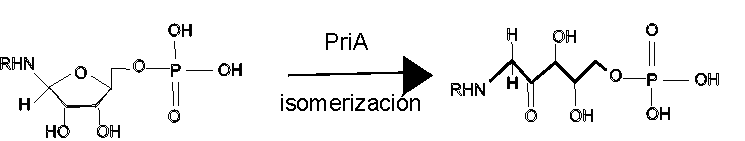
\includegraphics[angle = 0,scale = 1]{chapter4/isomerizacion.pdf}
  \caption[La reacción que cataliza PriA es una isomerización donde abre un anillo de cinco carbonos.]{\footnotesize{La reacción que cataliza PriA es una isomerización donde abre un anillo de cinco carbonos.}}
  \label{fig:isomerizacion}
  \end{figure}
  
  En este capítulo usamos como modelo de una familia promiscua la familia
  de PriA/HisA porque además PriA ha mostrado un gradiente funcional en
  Actinobacteria. Esta variación divide a la familia en varias subfamilias
  según su capacidad catalítica en los sustratos ProFAR y PRA. La
  evolución de las subfamilias de PriA y sus funciones es compleja y
  muestra dinámicas distintas en cada linaje (ver introducción). Por
  ejemplo incluye a los de miembros de PriB, la subfamilia ubicada en el
  género \emph{Streptomyces} con baja capacidad de catálisis para la
  función TrpF. Varios \emph{Streptomyces} con un ortólogo en la familia
  PriB, se diferencian de otras Actinobacterias en que contienen en su
  genoma un gen \emph{trpF} localizado fuera del contexto genómico
  inmediato de los operones de histidina y triptofano. Otra subfamilia de
  PriA es subHisA, que ha perdido totalmente la actividad TrpF, existen
  miembros de subHisA en \emph{Corynebacteria} y en \emph{Actinomyces}.
  Finalmente en Actinomyces también encontramos la subfamilia
  \emph{subTrpF} que ha perdido la actividad de HisA.
  
  En este capítulo se exploran cuatro apectos de la familia PriA.
  \emph{i)} La distribución y el contexto genómico de PriA en diversos
  linajes genómicos. \emph{ii)} La información contenida a nivel de
  aminoácidos en variantes de PriA como medio de estudio de rutas
  evolutivas y su relación con la reconstrucción de su estructura
  tridimensional. \emph{iii)} Las posibles afinidades de PriA por otros
  sustratos con métodos bioinformáticos, y finalmente \emph{iv)} La
  validación experimental de la actividad de PriA con sus sustratos PRA,
  ProFAR o combinaciones de los dos.
  
  \section{La familia PriA cambió su función y sus patrones de
  promiscuidad en los cuatro linajes
  analizados}\label{la-familia-pria-cambio-su-funcion-y-sus-patrones-de-promiscuidad-en-los-cuatro-linajes-analizados}
  
  \subsection{Las expansiones no son condición necesaria para la
  promiscuidad}\label{las-expansiones-no-son-condicion-necesaria-para-la-promiscuidad}
  
  Para explorar PriA en diversos linajes genómicos se utilizaron las
  herramientas EvoMining y CORASON descritas en los capítulos previos. Se
  investigaron las expansiones de la familia PriA en los linajes
  Actinobacteria, Cyanobacteria, \emph{Pseudomonas} y Archaea. En la
  \autoref{fig:PriA_Expansiones} se muestra el número promedio de copias
  por genoma en los linajes genómicos seleccionados. En Actinobacteria,
  donde se sabe que PriA es promiscua no se detectaron copias extra. Según
  EvoMining en Actinobacteria no hay expansiones, prácticamente todas las
  copias son reconocidas como de metabolismo central (rojo o morado)
  aunque algunas PriA además son marcadas por antiSMASH como parte de
  algún cluster biosintético (morado). En cambio en Cyanobacteria,
  \emph{Pseudomonas} y Archaea la figura muestra en negro las copias extra
  de las que no se conoce su destino metabólico. El caso de Archaea es
  llamativo porque las copias de metabolismo central llegan en promedio
  hasta .5 copias por genoma, es decir muchos genomas de Archaea no
  cuentan con una copia de PriA, y en cambio, contrario a Actinobacteria,
  un 50\% de la copias es marcado en negro, es decir varios de los genomas
  que tienen al menos una copia de PriA en realidad tienen dos copias.
  Esta figura muestra que en Actinobacteria PriA consituye un ejemplo de
  familia promiscua mayoritariamente distribuida con una sola copia por
  genoma por lo que es evidente que para que una familia sea promiscua no
  es imperativo tener copias extra con marcas de reclutamiento en
  metabolismo especializado. Aunque las copias extra suelen ser una
  indicación de promiscuidad, no son una condición necesaria. Tanto
  EvoMining como CORASON mostraron que existen excepciones de organismos
  donde PriA tiene doble copia, tanto en Actinobacteria como en otros
  linajes genómicos.
  
  \begin{figure}[h!tbp]
  \centering
  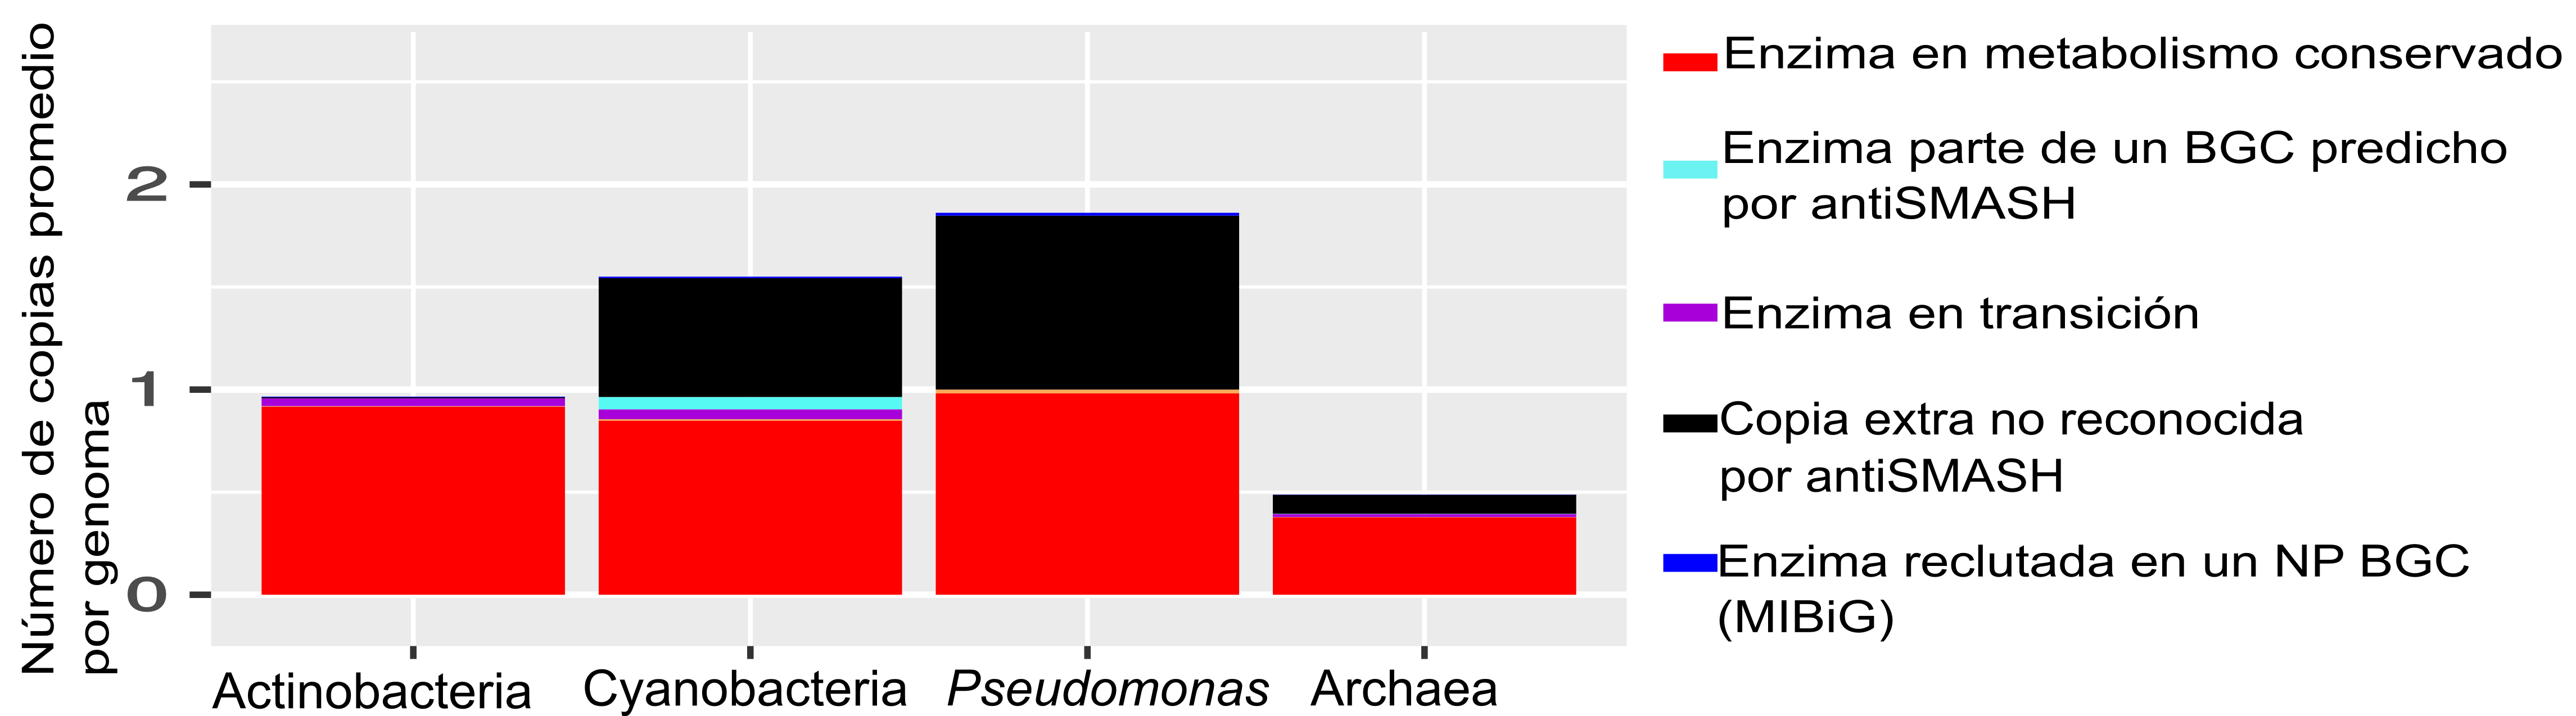
\includegraphics[angle = 0,scale = 0.8]{chapter4/PriAExpansiones.png}
  \caption[Expansiones de PriA en Actinobacteria, Cyanobacteria, Pseudomonas y Archaea]{\footnotesize{Número promedio de copias por genoma de PriA en Actinobacteria, Cyanobacteria, Pseudomonas y Archaea. Los colores muestran el destino metabólico asignado a cada copia según EvoMining. En rojo están los BBH a las enzimas semilla de metabolismo central. En morado las enzimas de metabolismo central también reconocidas por antiSMASH como parte de unBGC y en negro las copias sin un destino metabólico conocido.}}
  \label{fig:PriA_Expansiones}
  \end{figure}
  
  \subsection{Las expansiones condujeron a la creación de la subfamilia
  HisF}\label{las-expansiones-condujeron-a-la-creacion-de-la-subfamilia-hisf}
  
  Después del conteo de número de copias promedio, se analizaron los
  árboles de PriA de EvoMining coloreados de acuerdo al número de copias,
  \autoref{fig:PriAEvoMiningCopies}En Actinobacteria la mayoría de las
  hojas son verdes mostrando que existe sólo una copia por genoma en ese
  organismo. Sin embargo, existen varias hojas de color amarillo, lo que
  indica que hay dos copias en algunos genomas. En Cyanobacteria,
  \emph{Pseudomonas} y Archaea en contraste con Actinobacteria, se
  muestran una mezcla entre organismos que poseen una (verdes) o dos
  copias (amarillos) de PriA. Sin embargo al analizar detalladamente los
  árboles producidos por EvoMining en los distintos linajes, tanto en
  Cyanobacteria como en \emph{Pseudomonas} la copia extra está en una rama
  divergente y muy poblada del árbol de esta Familia Expandida, lo que
  indica que esas copias extra son en realidad miembros de otra subfamilia
  enzimática que aun guarda cierta similitud de secuencia con PriA. Esta
  segunda copia está en su mayoría anotada por RAST como imidazol glicerol
  fosfato sintasa ciclasa en ambos linajes. En Archaea sin embargo,
  diversas especies de la clase Methanomicrobia sí tienen dos copias
  cercanas a PriA.
  
  \begin{figure}[h!tbp]
  \centering
  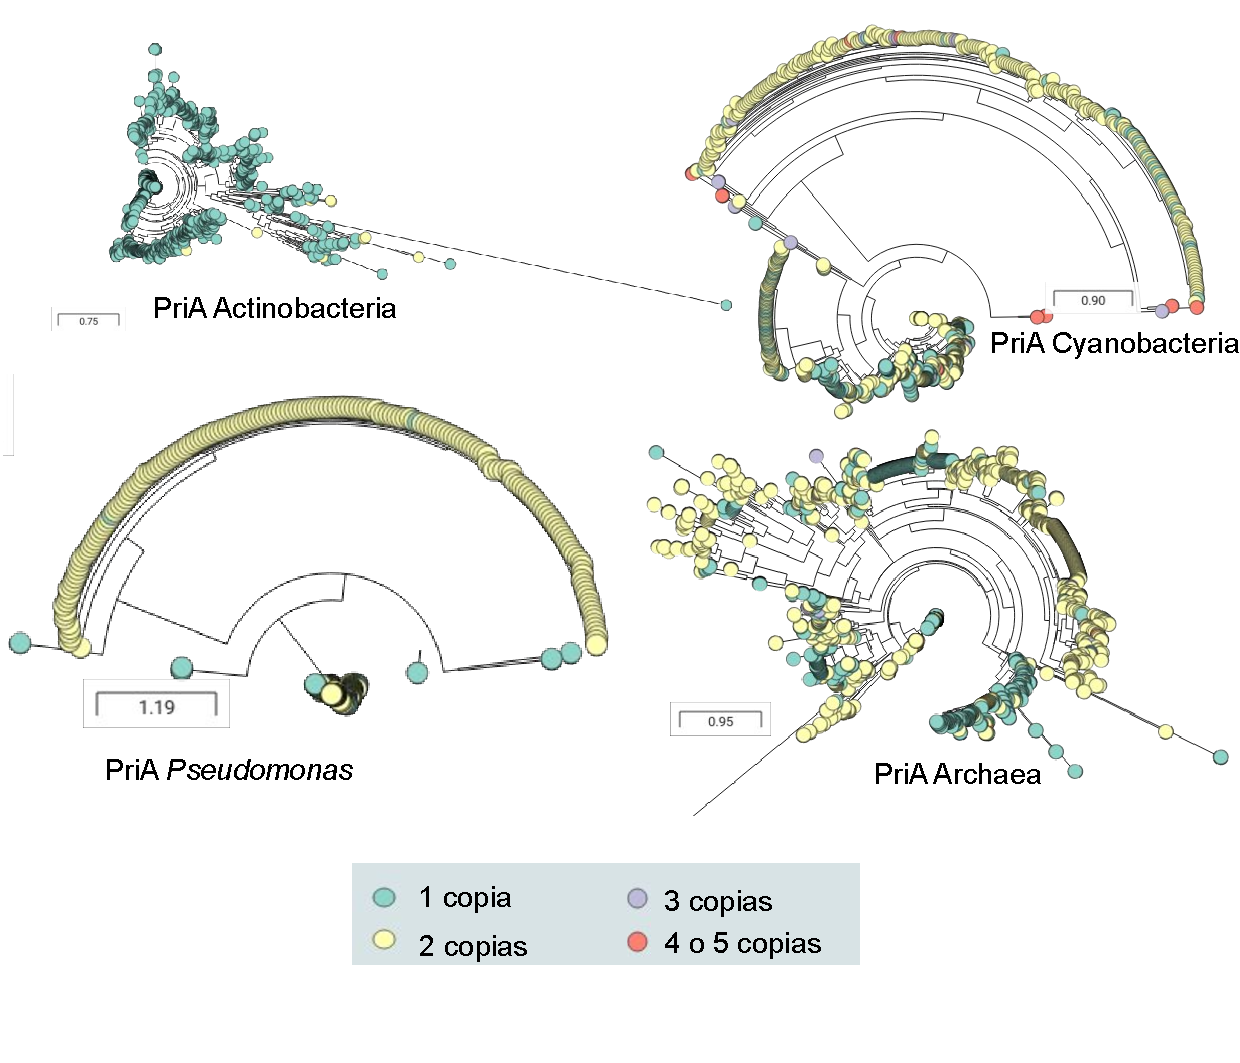
\includegraphics[angle = 0,scale = 0.8]{chapter4/PriAEvoMiningCopies.pdf}
  \caption[Copias extras de PriA en Actinobacteria, Cyanobacteria, {Pseudomonas} y Archaea]{\footnotesize{Número de copias de PriA en Actinobacteria, Cyanobacteria, {Pseudomonas} y Archaea. En Actinobacteria, donde se ha comprobado su promiscuidad enzimática la moda en el número de copias es uno (verde). En Cyanobacteria y Archaea se observa una mezcla de hojas verdes y hojas amarillas, donde las amarillas son nodos que pertenecen a organismos con dos copias. También en estos linajes algunos organismos poseeen tres copias (morado) y cuatro o cinco (rojo). En {Pseudomonas} la mayoría de los organismos muestran dos copias}}
  \label{fig:PriAEvoMiningCopies}
  \end{figure}
  
  \subsection{Cada linaje tiene distintos destinos metabólicos de
  PriA}\label{cada-linaje-tiene-distintos-destinos-metabolicos-de-pria}
  
  Después de explorar cuáles organismos tienen expansiones de PriA,
  analizamos el posible destino metabólico de las copias extra de la
  familia como se muestra en la \autoref{fig:PriATrees}. El árbol de
  Actinobacteria está poblado de hojas rojas \autoref{fig:PriATrees}, es
  decir de PriA dedicadas al metabolismo conservado, en este caso
  relacionado a las rutas de Histidina y Triptofano. Sin embargo hay
  algunas hojas grises, como es el caso de los dos \emph{Serenicoccus}. Es
  posible que estas PriA puedan tener funciones alternativas o ser otros
  eventos con cambio de promiscuidad. Además, en Actinobacteria la PriA de
  \emph{Janibacter hoilley}, la rama más larga del árbol, es muy
  divergente. Esto se debe a que existe una fusión de PriA con HisH. La
  fusión de genes bacterianos es un mecanismo común para formar proteínas
  multidominio {[}\protect\hyperlink{ref-pasek_gene_2006}{138}{]}. De
  hecho, dentro del operon de histidina existen fusiones reportadas HisNB
  y HisIE con proteínas bifuncionales en ciertas proteobacterias
  {[}\protect\hyperlink{ref-fani_origin_2005}{139}{]}. La fusión aquí
  presentada no parece ser un artefacto de anotación ya que hay otros
  genomas de \emph{Janibacter} con secuencias de PriA más grandes que el
  promedio. Los árboles que se produjeron por EvoMining están disponibles
  para exploración interactiva en Microreact en los links de la
  \autoref{tab:arboles}:
  
  En Cyanobacteria hay pocas predicciones de EvoMining, lo que se muestra
  en escasas hojas verdes \autoref{fig:PriATrees} que además no están
  localizadas cerca de su reclutamiento la HisA de saxitoxin, el BGC
  proveniente de Cyanobacteria. Varias de las copias extra de
  Cyanobacteria corresponden a HisF, la subunidad enzimática imidazol
  glicerol fosfato sintasa parte también del operón de histidina. HisA
  proviene de una duplicación de un ancestro común de la mitad de su
  tamaño y HisF proviene de la duplicacion de HisA
  {[}\protect\hyperlink{ref-fani_evolution_1994}{140}{]}. Por ello puede
  considerarse que EvoMining en efecto está encontrando una expansión de
  HisA que consiste en la familia HisF en el linajes Cyanobacteria, lo
  mismo ocurre en \emph{Pseudomonas}. En su momento HisF fue parte del
  \emph{dispensable genome}, no todos los organismos poseían esta
  expansión, posteriormente, al parecer antes del último ancestro común de
  Archaea, Bacteria y Eukarya, la síntesis de histidina fue fijada
  {[}\protect\hyperlink{ref-fondi_evolution_2009}{44}{]}. Este es un caso
  donde lo que alguna vez fue \emph{dispensable genome} / metabolismo
  secundario, se ha vuelto \emph{shell genome} / metabolismo conservado y
  donde se muestra que en estos linajes Cyanobacteria y \emph{Pseudomonas}
  EvoMining aún es capaz detectar esa marca de expansión. De hecho se ha
  reconstruido una HisF ancestral con el objetivo de probar si retenía la
  actividad de HisA, es decir si poseía promiscuidad enzimática
  {[}\protect\hyperlink{ref-merkl_reconstruction_2016}{142}{]}. LUCA-HisF
  mostró no ser promiscua para los sustratos de HisA ni tampoco para su
  similar el sustrato TrpF.
  
  En \emph{Pseudomonas} hay una gran población de predicciones de
  EvoMining, pero el árbol tiene similitudes con Cyanobacteria, la rama
  divergente corresponde en su mayoría a copias de HisF. De hecho, el
  reclutamiento que hace que el árbol de \emph{Pseudomonas} tenga una rama
  verde está anotado funcionalmente no como una HisA, sino como una
  \href{https://www.ncbi.nlm.nih.gov/protein/CAB65215.1/}{HisF} parte de
  un BGC que produce un lipopolisacárido en la Proteobacteria
  \emph{Legionella pneumophila}. En Archaea, la rama central con una
  mezcla de hojas grises y rojas \autoref{fig:PriATrees} contiene también
  copias de HisF provenientes de genomas de \emph{Sulfolobus}. Al verficar
  en el árbol interactivo en Microreact \autoref{tab:arboles} el número de
  copias presente en organismos con un homólogo clasificado como HisF se
  comprobó que los \emph{Sulfolobus} sólo poseen una copia en este árbol.
  Sin embargo, tanto al explorar manualmente los genomas de
  \emph{Sulfolobus}, como al revisar la literatura sobre metabolismo de
  histidina en Archaea se encontró que sí se han encontrado homólogos de
  PriA en genomas de \emph{Sulfolobus}
  {[}\protect\hyperlink{ref-fondi_evolution_2009}{44}{]}. Por tanto este
  árbol sugiere que aunque existe tanto PriA como su expansión HisF en el
  género \emph{Sulfolobus}, la copia HisF es la más parecida a la semilla
  con que se generó este árbol. Además la similitud de secuencia del
  homólogo de HisA no fue suficiente para recuperar copias de HisA en este
  experimento computacional. Algunas de los hojas grises del árbol sin
  destino metabólico conocido serán exploradas en la siguiente sección.
  
  \begin{figure}[h!tbp]
  \centering
  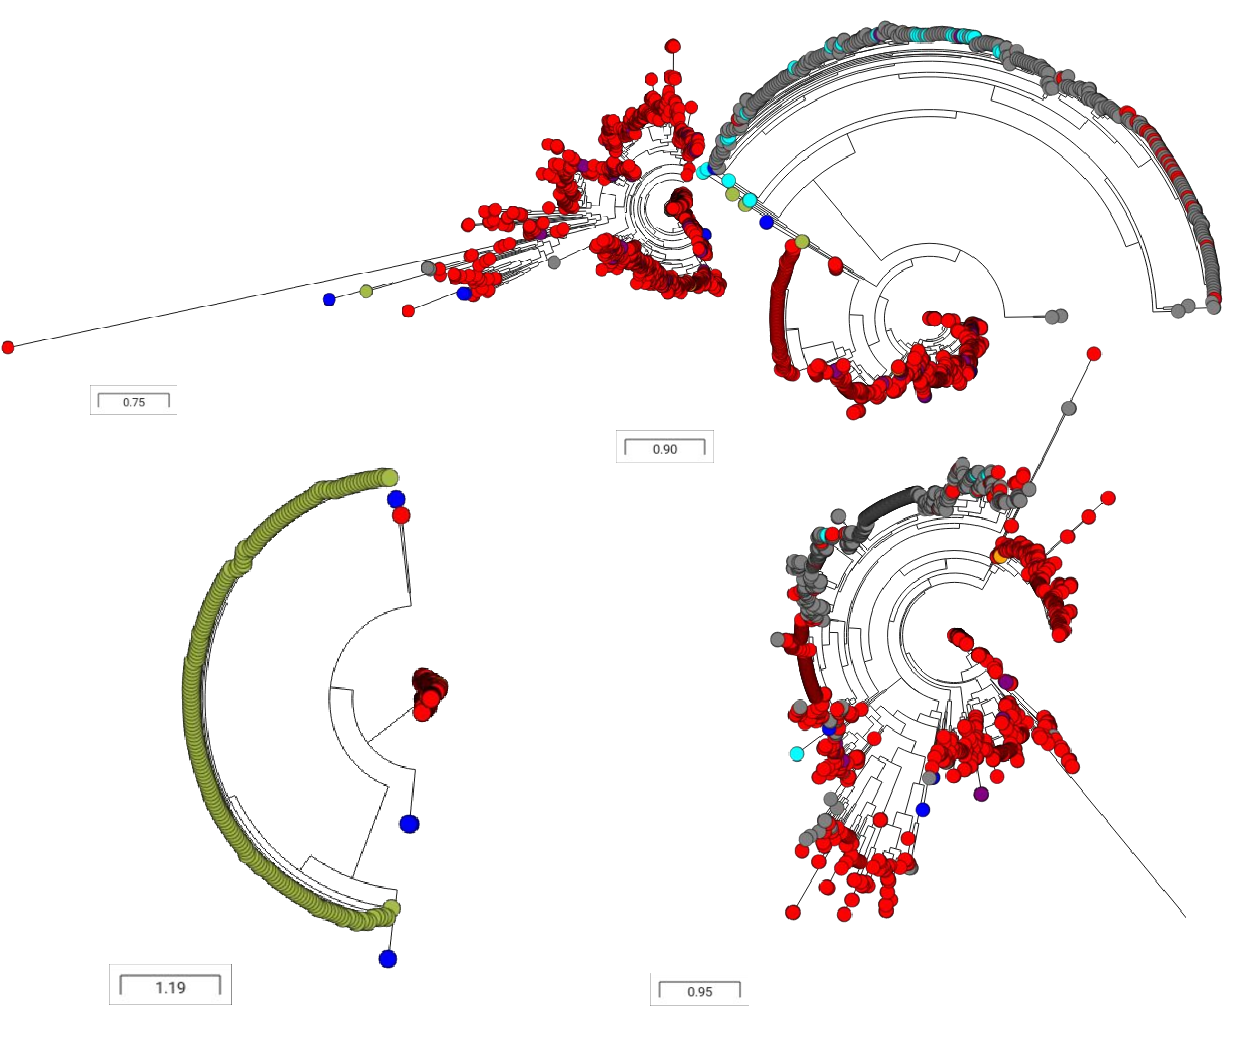
\includegraphics[angle = 0,scale = 0.8]{chapter4/PriAEvoMining.pdf}
  \caption[Árboles de destino metabólico de PriA en Actinobacteria, Cyanobacteria, {Pseudomonas} y Archaea según EvoMining]{\footnotesize{Árboles de destino metabólico de PriA en Actinobacteria, Cyanobacteria, {Pseudomonas} y Archaea según EvoMining}}
  \label{fig:PriATrees}
  \end{figure}
  
  \begin{longtable}[]{@{}lc@{}}
  \caption{Árboles EvoMining de PriA/HisA en MicroReact
  \label{tab:arboles}}\tabularnewline
  \toprule
  Linaje & Link al árbol de EvoMining en Microreact\tabularnewline
  \midrule
  \endfirsthead
  \toprule
  Linaje & Link al árbol de EvoMining en Microreact\tabularnewline
  \midrule
  \endhead
  Actinobacteria &
  \href{https://microreact.org/project/7g2IGfkv9}{7g2IGfkv9}\tabularnewline
  Cyanobacteria &
  \href{https://microreact.org/project/qF6jWRMox}{qF6jWRMox}\tabularnewline
  \emph{Pseudomonas} &
  \href{https://microreact.org/project/ydff6DWqs}{ydff6DWqs}\tabularnewline
  Archaea &
  \href{https://microreact.org/project/Ig-m9Cm6f}{Ig-m9Cm6f}\tabularnewline
  \bottomrule
  \end{longtable}
  
  \subsubsection{Homólogos de PriA han sido reclutados a clusters de
  metabolismo
  especializado}\label{homologos-de-pria-han-sido-reclutados-a-clusters-de-metabolismo-especializado}
  
  Se encontraron algunos homólogos reclutados a BGC conocidos, marcados en
  azul en el árbol, que son miembros de la familia expandida PriA/HisA en
  estos linajes genómicos. La información de dichos BGC está listada en la
  tabla \autoref{tab:reclutamientos}. Entre ellos se encuentran dos
  toxinas de Cyanobacteria
  {[}\protect\hyperlink{ref-moustafa_origin_2009}{143}{]}, un
  lipopolisacárido producido por una Proteobacteria y un BGC productor de
  cloro-pentostatina producido en Actinobacteria
  {[}\protect\hyperlink{ref-gao_biosynthesis_2017}{144}{]}.
  
  Table: Reclutamientos de expansiones de PriA en MIBiG
  \label{tab:reclutamientos}\\
  \[
  \resizebox{\columnwidth}{!}{%
  \begin{tabular}{ l c c c}
  \hline \\ [-1.5ex]  
  Compuesto & Organismo & BGC origen & Clase \\ [1ex]  
  \hline \\ [-1.5ex]
  \href{http://mibig.secondarymetabolites.org/repository/BGC0001484/index.html\#cluster-1}{Pentostatina}&\textit{Actinomadura} sp. ATCC 39365&Actinobacteria& Otros     \\ [1ex]  
  \href{http://mibig.secondarymetabolites.org/repository/BGC0000188/index.html\#cluster-1}{Saxitoxina}&\textit{Cylindrospermopsis~raciborskii} T3&Cyanobacteria&Alcaloide \\ [1ex]  
  \href{http://mibig.secondarymetabolites.org/repository/BGC0000928/index.html\#cluster-1}{Toxina }&\textit{Dolichospermum~circinale} AWQC131C & Cyanobacteria & Otros    \\ [1ex]  
  \href{http://mibig.secondarymetabolites.org/repository/BGC0000775/index.html\#cluster-1}{Lipopolisacárido}  &\textit{Legionella~pneumophila}    & Proteobacteria & Sac\'arido    \\ [1ex]  
  \hline
  \end{tabular}}
  %}
  \] \normalsize
  
  La pentostatina es un antibiótico nucleosídico derivado de adenosina,
  cuyo cluster es llamado \emph{ada} . La PriA del cluster \emph{ada} es
  llamada \emph{adaK} y sí parece participar del cluster, ya que muestra
  una isomerización sobre un sustrato similar a los nativos de PriA,
  \autoref{fig:ada}, con un anillo de 5 carbonos, dos OH, un oxígeno y un
  grupo fosfato . Esta isomerización es muy parecida a la que realiza PriA
  sobre ProFAR y PRA. Esta PriA no es una copia extra, sino la copia única
  de este organismo. Este contexto genómico no se encuentra conservado en
  las copias vecinas en el árbol. Es relevante mencionar que la mutante de
  PriA no suprime la producción de este antibiótico en \emph{Actinomadura}
  sp. ATCC 39365, por lo que los autores especulan que otra enzima podría
  estar realizando la isomerización redundantemente. \emph{Actinomadura}
  no posee una copia de TrpF que sería el candidato inmediato.
  
  \begin{figure}[h!tbp]
  \centering
  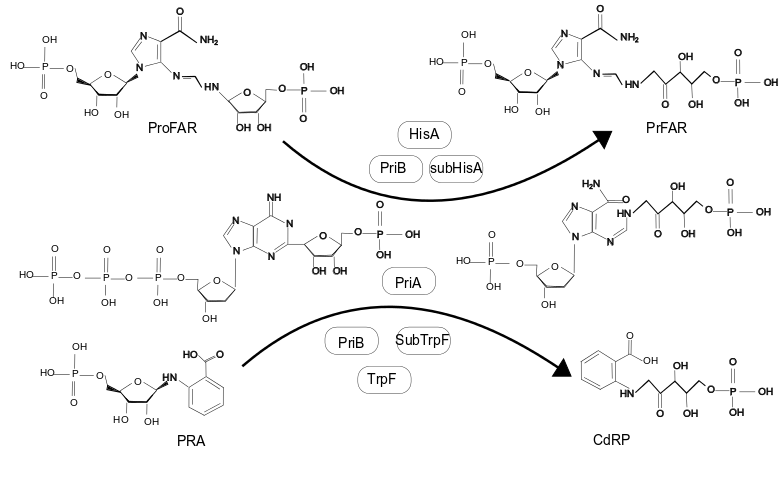
\includegraphics[angle = 0,scale = 0.6]{chapter4/ada.png}
  \caption[PriA participa en la síntesis del antibiótico {ada} en {Actinomadura} ]{\footnotesize{PriA participa en la síntesis del antibiótico {ada} en {Actinomadura}. Los sustratos nativos de Pria, ProFAR y PRA son isomerizados de manera muy similar a un paso en la ruta de síntesis de {ada} }}
  \label{fig:ada}
  \end{figure}
  
  \clearpage
  
  \section{Análisis de contextos genómicos de PriA/HisA en distintos
  linajes utilizando CORASON como herramienta de
  visualización.}\label{analisis-de-contextos-genomicos-de-priahisa-en-distintos-linajes-utilizando-corason-como-herramienta-de-visualizacion.}
  
  \subsection{Contextos genómicos de HisA en
  Actinobacteria}\label{contextos-genomicos-de-hisa-en-actinobacteria}
  
  En Actinobacteria, se observó que todos los \emph{Streptomyces} tienen
  el cluster de PriA parcialmente conservado con respecto al BGC de
  \emph{Streptomyces coelicolor}. Ejemplos de ello son \emph{S. roseous},
  \emph{S. sviceus}, \emph{S. sp C} y \emph{S. Mg1} donde genes tanto de
  la ruta de histidina como de triptofano rodean a PriA. Otros como
  \emph{S rimosus} , \emph{S HmicA12} y \emph{S. sp CT34} tienen los genes
  de triptofano más alejados \autoref{fig:ActinoCORASON} . Como ya se
  describió en la sección de EvoMining, el único organismo de este género
  con una copia extra de PriA es \emph{Streptomyces} CT34. Esta copia
  parece deberse a transferencia horizontal dado que su mejor hit en NCBI
  proviene de una \emph{Lentzea}. Aún así parece ser un homólogo lejano ya
  que tuvo 50\% de identidad en 98\% de cobertura con respecto a la copia
  de \emph{Lentzea}. Otro caso interesante en Actinobacteria son las
  Actinomaduras, ya que CORASON muestra que el cluster \emph{ada} no está
  conservado en ellas (datos no mostrados). Además, también en
  Actinobacteria CORASON muestra en \emph{Sporichthya polymorpha} DSM
  43042 una PriA precedida por una NRPS, una enzima por excelencia de
  productos naturales. En otros organismos antiSMASH predice que PriA
  forma parte de clusters putativos, por ejemplo en \emph{Modestobacter
  marinus} NC\_0179551, \emph{Geodermatophilus obscurus}, y en
  \emph{Streptacidiphilus jeojiense}. Los contornos de los genes
  reconocidos por antiSMASH como parte de un BGC son marcados en azul en
  las figuras de CORASON.
  
  \begin{figure}[h!tbp]
    \centering
    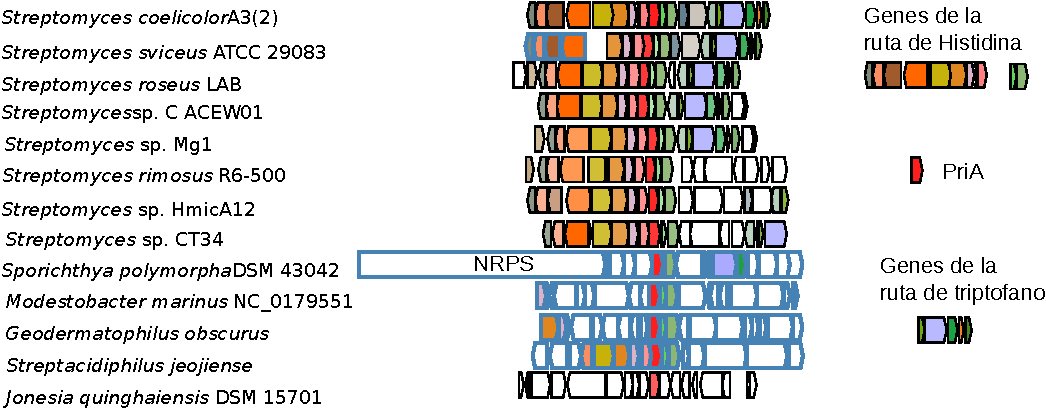
\includegraphics[angle = 0,scale = 0.9]{chapter4/CORASON/ActinoCORASON.pdf}
    \caption[Contextos de PriA en Actinobacteria]{\footnotesize{Contextos de PriA en Actinobacteria}}
    \label{fig:ActinoCORASON}
    \end{figure}
  
  \subsection{Contextos genómicos de HisA en
  Archaea}\label{contextos-genomicos-de-hisa-en-archaea}
  
  En cuanto al contexto de HisA en Archaea la \autoref{fig:ArchaeaCORASON}
  muestra que existen contextos como los de \emph{Thermococcus
  kodakarensis KOD1} y \emph{Thermococcus sp JCM 11816} donde \emph{hisA}
  está rodeada de genes tanto de histidina como de triptofano. Sin embargo
  esta configuración conjunta no es la generalidad. En Archaea, se conocen
  tres escenarios para la organización de los genes de síntesis de
  histidina. En el primero los genes de síntesis están dispersos en el
  genoma. El segundo escenario es la existencia de suboperones pequeños
  como \emph{hisHAF} y finalmente el tercer escenario es el operón con la
  mayoría de los genes juntos aunque no siempre en el mismo orden
  {[}\protect\hyperlink{ref-fondi_evolution_2009}{44}{]}.
  
  En efecto en Euryarchaeota están presentes los tres escenarios, en
  \emph{Archaeoglobales} y \emph{Halobacteriales} los genes del operón
  \emph{his} están distribuidos en el genoma, como muestran los contextos
  de \emph{hisA} en \emph{Halorubrum tebenquichense} y \emph{Halonotius
  sp.} sin ningún otro gen del operón cerca. En \emph{Thermosarcinales}
  donde ya se conocía la existencia del suboperón \emph{hisGBA}, se
  observó que éste se encuentra conservado en la mayoría de los miembros
  del orden como ejemplifica el contexto correspondiente a
  \emph{Methanosarcina lacustris}. En \emph{Thermococcales} se conocía la
  configuración \emph{hisGDBHAFIEC} que es confirmada por los tres
  \emph{Thermococcus} de la \autoref{fig:ArchaeaCORASON}, donde además se
  muestran dos contextos acompañados del su operón de triptofano
  \emph{trpCDEGF}, resultando un contexto total de
  \emph{hisGDBHAFIECXtrpCDEGF}. En el phylum Thaumarchaeota se habían
  estudiado sólo dos organismos y estos presentaban la configuración
  \emph{hisGDCXBHAI}. En contraste en este trabajo encontramos en el orden
  \emph{Nitrosopumilales} la configuración \emph{hisDCXBHAFIE}, donde
  además la \emph{hisX} es una fosfatasa homóloga a la \emph{hisX}
  presente en \emph{T. kodakarensis} . Este patrón es común en
  Thaumarchaeota, aunque también se muestra la existencia del suboperón
  \emph{hisAF} en \emph{Aigarchaeota} así como la configuración de genes
  dispersos en el genoma en \emph{Thaumarchaeota archaeon JGI OTU-1}. En
  Crenarchaeota \emph{hisCGABFDEHI} está presente según la anotación
  funcional de RAST, aunque no todos los genes aparecen en color en la
  figura debido a la baja identidad de secuencia que conservan con
  respecto al contexto de referencia de \emph{T. kodakarensis}. En
  \emph{Pyrobaculum neutrophilum} está parcialmente conservado el operón
  con la configuración \emph{hisCEDFBA}, nuevamente con algunos genes con
  baja identidad de secuencia respecto a \emph{T. kodakarensis}. La
  configuración genes dispersos en el cromosoma en el phylum Crenarchaeota
  es mostrada en el contexto de \emph{Ignicoccus islandicus}. Finalmente
  fue analizado el contexto de \emph{hisA} en Bathyarchaeota un phylum
  donde no se contaba con información previa. En Bathyarchaeota se
  conserva como en Thaumarchaeota el ordenamiento \emph{hisGDCXBHAI},
  aunque existen otras configuraciones como muestra \emph{Bathyarchaeota
  archaeon B25}.
  
  Otra característica interesante de la visualización de los contextos de
  HisA en Archaea es que los tamaños de \emph{hisA} son más variados que
  en Actinobacteria. Esta característica se debe tanto a variación
  intrínseca del tamaño de \emph{hisA} como a diversas fusiones. Por
  ejemplo en \emph{Halonotius sp J07HN6} \emph{hisA} se encuentra
  fusionada con \emph{flaJ} una proteína relacionada con la construcción
  de flagelos en Archaea. En Candidatus \emph{Bathyarchaeota archaeon
  B26-1} \emph{hisA} se muestra fusionada con \emph{hisF}.
  
  En conclusión, no encontramos una configuración conservada que
  prevalezca en todo Archaea. Esto puede deberse a que Archaea es un
  dominio, no un phylum como Actinobacteria, y por tanto hay una mayor
  distancia entre los organismos que la conforman. Queda por
  
  \begin{figure}[h!tbp]
  \centering
  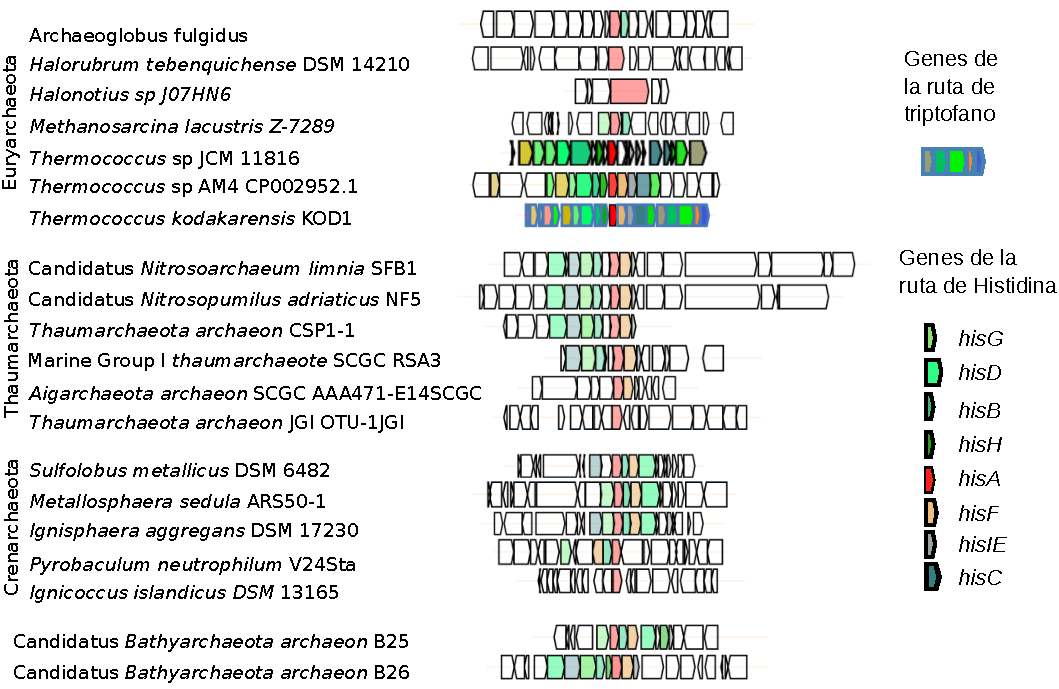
\includegraphics[angle = 0,scale = 0.8]{chapter4/CORASON/ArchaeaCORASON.pdf}
  \caption[Contextos de PriA en Archaea]{\footnotesize{Contextos de PriA en Archaea}}
  \label{fig:ArchaeaCORASON}
  \end{figure}
  
  \subsection{Contextos genómicos de HisA en
  saxitoxin}\label{contextos-genomicos-de-hisa-en-saxitoxin}
  
  Como se mostró en la sección de análisis de expansiones de HisA con
  EvoMining en Cyanobacteria, \emph{hisA} aparece dentro del cluster
  reportado como productor de saxitoxina en MIBiG. El contexto que rodea
  al reclutamiento de \emph{hisA} en el cluster de saxitoxina no está
  conservado en Cyanobacteria según la visualización de contextos
  producida por CORASON. Tomando como semilla la secuencia de HisA del BGC
  de saxitoxina y como referencia el cluster de saxitoxina, se muestra que
  si bien los reguladores del BGC saxitoxina sí están conservados en la
  vecindad genómica de HisA en otros organismos, este no es el caso para
  las enzimas biosintéticas del \emph{cluster}. Además en el lado
  izquierdo de la \autoref{fig:saxitoxin} se muestra que la HisA del BGC
  saxitoxina no está ubicada en una rama de PriA divergente, al contrario
  está embebida en la parte más conservada. Por estas razones es posible
  que PriA esté en la orilla del BGC de saxitosina y más bien no participe
  en la síntesis de este compuesto o bien que mantenga su función primaria
  y a la ve tenga una función aún desconocida teniendo un papel en la
  regulación de la producción de saxitosina.
  
  \begin{figure}[h!tbp]
  \centering
  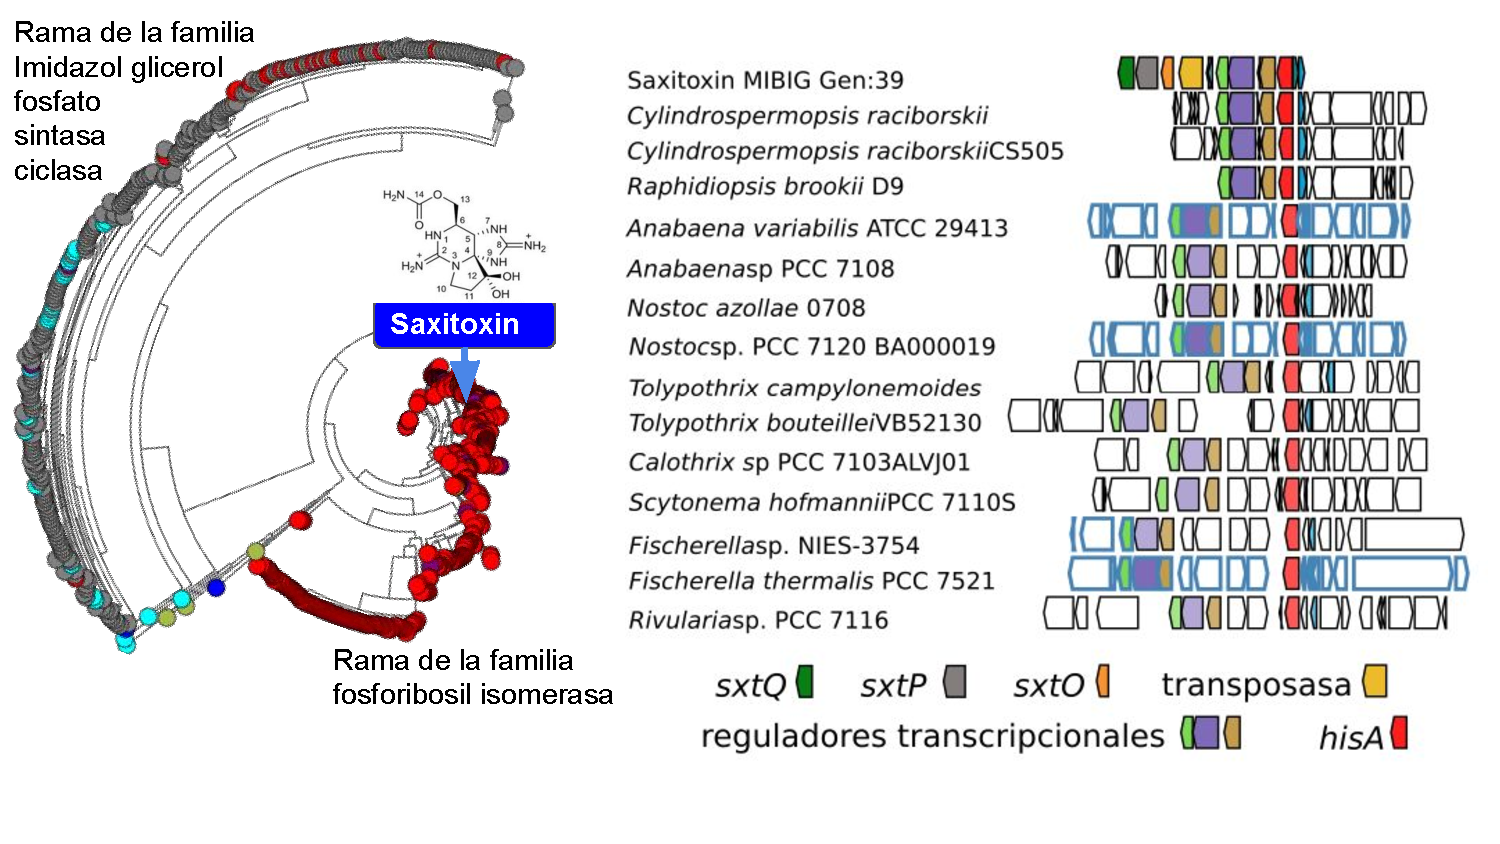
\includegraphics[angle = 0,scale = 0.7]{chapter4/CORASON/saxitoxin.pdf}
  \caption[HisA en saxitoxin, un cluster de Cyanobacteria ]{\footnotesize{HisA en saxitoxin, un cluster de Cyanobacteria }}
  \label{fig:saxitoxin}
  \end{figure}
  
  \section{Evolución molecular y estructural de
  PriA}\label{evolucion-molecular-y-estructural-de-pria}
  
  En esta segunda sección concerniente a la familia PriA se busca
  información contenida en la secuencia de aminoácidos. En la primera
  parte se discute cómo en datos de evolución dirigida en el laboatorio no
  se encontró ninguna trayectoria en donde algún paso incrementara la
  actividad de PriA en sus dos sustratos nativos. En la segunda parte se
  muestra una reconstrucción de la estructura tridimensional de PriA
  basada en la covarianza de sus aminoácidos en secuencias del registro
  evolutivo.
  
  \subsection{Al transformar una subHisA en una PriA mediante mutaciones
  no se observó ninguna trayectoria creciente para ambos
  sustratos}\label{al-transformar-una-subhisa-en-una-pria-mediante-mutaciones-no-se-observo-ninguna-trayectoria-creciente-para-ambos-sustratos}
  
  En esta sección analizamos cómo cambia la capacidad catalítica de PriA
  sobre un sustrato mientras se varía la del otro. Para ello se utilizaron
  datos de mutantes de subHisA de \emph{Corynebacterium diphteriae}. Estas
  mediciones de cinéticas enzimáticas fueron obtenidos del trabajo de
  tesis de Lianet Noda {[}\protect\hyperlink{ref-noda_tesis_2012}{75}{]}.
  A partir de la secuencia original que se mostró es una subHisA, se
  realizaron mutantes con el objetivo de alcanzar la promiscuidad, es
  decir de convertir la enzima subHisA en una PriA. Se comenzó con
  diferentes mutantes puntuales adicionando una mutación cada vez, hasta
  llegar a una con 11 mutaciones. En esta colección de mutantes varias
  ganaron la función de PRA isomerasa, a distintos niveles. La que alcanzó
  mayor actividad PRA isomerasa fue la \(9.3\), una variante con nueve
  mutaciones. En estos datos quedaba pendiente la exploración de los
  caminos mutacionales, es decir cómo es el camino desde una mutante
  sencilla hasta una múltiple ¿cuántas rutas son posibles? ¿Existe alguna
  tendencia en ciertos momentos de la ruta sobre el incremento/decremento
  de alguna de las dos funciones?
  
  Asi pues se desarrolló un
  \href{https://github.com/nselem/perlas/tree/master/LiaTrayectory}{programa}
  utilizando recursividad para reconstruir todas las rutas posibles. El
  total de rutas calculadas hasta la mutación 11 fue de 2928 caminos, las
  rutas posibles hasta la mutante 9.3 son 790. Estas rutas son mostradas
  en la \autoref{fig:PriARutas}.
  
  \begin{figure}[h!tbp]
  \centering
  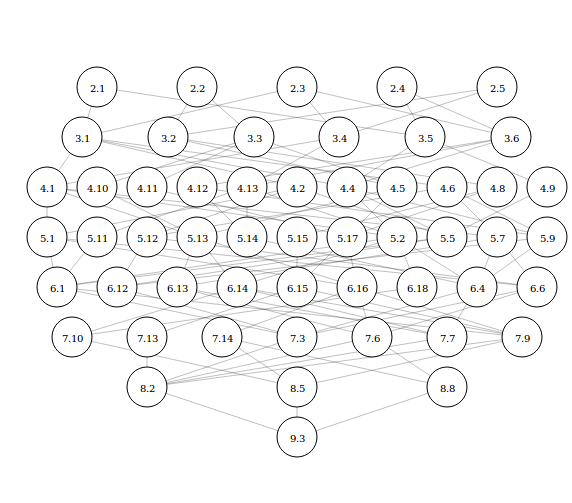
\includegraphics[angle = 0,scale = 0.6]{conclusion/Solocirculos.png}
  \caption[Rutas desde una subHisA hasta una variante con 9 mutaciones]{\footnotesize{Rutas desde una subHisA hasta una variante con 9 mutaciones. En cada círculo el primer dígito indica el número de mutaciones}}
  \label{fig:PriARutas}
  \end{figure}
  
  Al analizar todas las rutas que llevan a \(9.3\) se descubrió que no
  existe en ellas una trayectoria en la todos los pasos incrementen la
  actividad de TrpF. Por otra parte, se observa que a pesar de que la
  primera mutación siempre decrece la actividad de HisA, en pasos
  subsecuentes se observa que esta actividad se incrementa, lo que muestra
  que hay epistasis positiva o amortiguadora. Esto es que los efectos
  negativos que de las mutaciones sobre SubHisA pueden ser menos negativos
  o hasta positivos cuando las mismas mutaciones ocurren en una proteína
  que ya tiene otras mutaciones. Como ejemplo, en la
  \autoref{fig:PriARutas} se muestran las rutas donde cada mutante
  mantiene un nível mínimo de actividad de ProFAR isomerasa
  (\(\frac{K_{cat}}{K_m} PriA_{ProFAR} \ge .004\)). En azul sólido se ven
  los incrementos en PRA y en rojo sólido los incrementos en ProFAR. Las
  líneas punteadas indican que la actividad decreció en ese paso de la
  ruta. Entre una y cuatro mutaciones el azul sólido es predominante, es
  decir se incrementa la actividad para PRA, pero entre 4 y 5 mutaciones
  ningún paso incrementa la actividad de PRA y en cambio sí se incrementa
  la actividad para ProFAR, esta figura sugiere que al mejorar una
  actividad se compromete el mejoramiento de la otra. En este ejemplo, las
  mutaciones puntuales que llevan a una enzima monofuncional a adquirir
  promiscuidad no mantienen una tendencia no decreciente de principio a
  fin sobre ninguna ruta en ninguna de las dos reacciones isomerización de
  PRA e isomerización de ProFAR. Este tipo de trayectorias se conoce como
  no darwininana ya que siempre existe algún paso donde decrece alguna de
  las actividades.
  
  \begin{figure}[h!tbp]
  \centering
  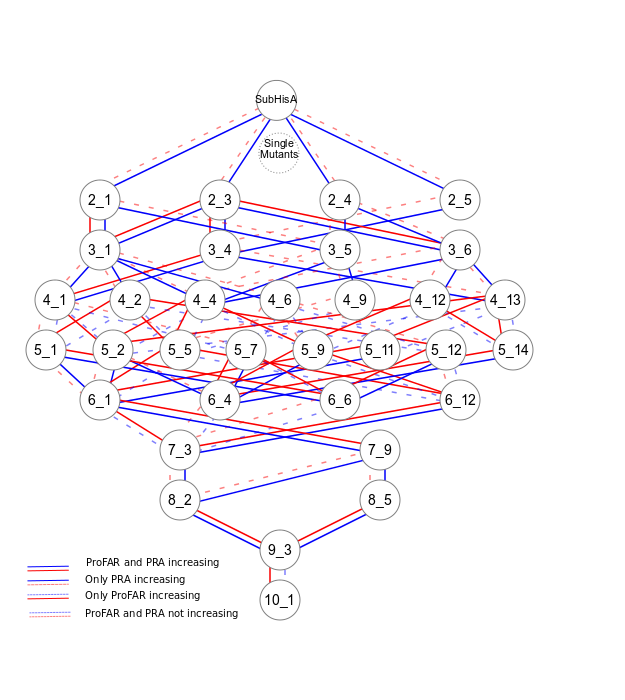
\includegraphics[angle = 0,scale = 0.7]{chapter4/LianetFiguras/SolocirculosPRA_PRO_RUTAS_10_1_r002.png}
  \caption[Positive increments on PRA]{\footnotesize{Rutas de evolución dirigida para ganar la función PRA. En la figura se muestra como la mayoría de los pasos que incrementan una función hacer decrecer la capacidad catalítica de la otra. El primer número de cada nodo indica cuántas mutaciones tiene esa variante y el segundo número es el identificador de esa combinación específica.}}
  \label{fig:PRARutas}
  \end{figure}
  
  \clearpage  
  
  \subsection{Los residuos que covarían en el registro evolutivo de PriA
  permiten una reconstrucción aproximada de su estructura
  tridimensional}\label{los-residuos-que-covarian-en-el-registro-evolutivo-de-pria-permiten-una-reconstruccion-aproximada-de-su-estructura-tridimensional}
  
  El estudio de la evolución de PriA en la sección anterior nos
  proporcionó el aprendizaje de que para adquirir una actividad el camino
  no es estrictamente creciente. En cambio, suele haber pasos donde alguna
  de las dos actividades baja. En esta sección utilizaremos el registro
  evolutivo resultado de millones de años, tomaremos miles de homólogos de
  PriA para inferir la estructura tridimensional de una secuencia.
  EVcouplings es un método que considera las secuencias génicas existentes
  como experimentos exitosos de la naturaleza. Con esta información
  obtiene la covariación entre pares de aminoácidos de las secuencias
  existentes en el registro evolutivo. Los pares fuertemente relacionados
  se denominan acoplamientos, estos acoplamientos a menudo están cerca
  físicamente en la estructura terciaria de la proteína. Se ha demostrado
  que muchas proteínas contienen suficientes acoplamientos distribuidos
  ampliamente en toda la secuencia, de forma que con ellos es posible la
  reconstrucción de su estructura tridimensional
  {[}\protect\hyperlink{ref-marks_protein_2011}{145}{]}. En esta sección
  se aplicará EVcouplings para reconstruir la estructura tridimensional de
  PriA.
  
  Las diferencias a nivel estructural pueden amplificar la información
  proporcionada por variaciones a nivel de secuencia. Una métrica común de
  distancia entre dos estructuras de proteínas es el \emph{root mean
  sqaured deviation} (RMSD). Esta distancia se obtiene después de alinear
  las estructuras calculando el promedio de las distancias al cuadrado
  entre los átomos de carbono primarios
  {[}\protect\hyperlink{ref-kufareva_methods_2012}{146}{]}. La información
  de las covariación entre residuos es suficiente para que el método
  EVcouplings genere estructuras con un error de 2.7--4.8 \({\AA}\)
  respecto a la estructura cristalográfica conocida
  {[}\protect\hyperlink{ref-marks_protein_2011}{145}{]}. Por este motivo
  se decidió implementar EVcouplings y aplicarlo a la familia PriA. Este
  método es de difícil instalación ya que requiere varias dependencias.
  Por ello, desarrollé un contenedor Docker donde dependencias, software y
  base de datos quedan instalados. Este desarrollo fue incluido por los
  autores de EVcouplings como sugerencia de instalación. El contenedor
  docker implementa el \emph{EVcouplings python framework}
  {[}\protect\hyperlink{ref-hopf_evcouplings_2019}{147}{]} que comprende
  cinco etapas para estudiar el análisis de coevolución de residuos de una
  familia de proteínas. Dichas etapas son i) Alineado, ii) análisis de
  acoplamiento, iii) plegamiento basado en acoplamientos iv) análisis de
  mutación y v) comparación con estructuras conocidas.
  
  EVcouplings fue aplicado a la secuencia de PriA de \emph{Streptomyces
  coelicolor} obtenida de la base de datos
  \href{https://www.uniprot.org/}{Uniprot} con identificador
  \href{https://www.uniprot.org/uniprot/P16250}{HIS4\_STRCO}. Los
  parámetros de EVcouplings se dejaron con su configuración inicial
  incluyendo el umbral de recuperación para las secuencias utilizadas en
  el alineamiento. Con este alineamiento, utilizando la información de los
  acoplamientos de sus aminoácidos, se obtuvo el modelo \emph{PriAEV} de
  la estructura tridimensional de PriA de \emph{S. coelicolor}.
  
  Ahora bien, \href{https://www.rcsb.org/structure/1vzw}{1VZW} es una
  estructura de PriA de \emph{S. coelicolor} obtenida mediante
  cristalografía {[}\protect\hyperlink{ref-kuper_twofold_2005}{148}{]}. En
  esta tesis calculé que el RMSD entre PriA
  (\href{https://www.rcsb.org/structure/1vzw}{1VZW}) y su homólogo lejano
  HisF (\href{http://www.rcsb.org/structure/2A0N}{2A0N} proveniente de
  \emph{Thermotoga maritima} es de 7.34\({\AA}\). Así mismo la distancia
  obtenida entre PriA (\href{https://www.rcsb.org/structure/1vzw}{1VZW}) y
  el modelo de TrpF \href{http://www.rcsb.org/structure/5LHE}{5LHE} de
  \emph{Thermococcus kodakaraensis} es de 12.088 \({\AA}\). Por tanto
  cualquier modelo existoso de PriA debe tener un RMSD menor que estas
  distancias con respecto al modelo 1VZW. La distancia entre la estructura
  PriAEV y HisF es de 5.603 \({\AA}\) y el RMSD entre PriAEV y TrpF es de
  12.554 \({\AA}\). Además, la distancia entre estas 1VZW y PriAEV medida
  utilizando el RSMD (pymol 2.2.3) entre ellas es de 3.362 \({\AA}\). Así
  pues PriAEV consigue diferenciarse de HisF y TrpF y estar a una
  distancia de 3.362 \({\AA}\) de 1VZW. Esta distancia es menor que que el
  3.730 \({\AA}\) el RMSD entre la estructura de PriA
  \href{https://www.rcsb.org/structure/1vzw}{1VZW} de \emph{S. coelicolor}
  y la estructura de PriA \emph{Streptomyces sviceus ATCC 29083} con
  identificador de PDB \href{https://www.rcsb.org/structure/4TX9}{4TX9}.
  Además, las estructuras cristalográficas tienen una resolución de 1-3
  \({\AA}\) como puede verse en la \autoref{tab:EnzymePDB}, por tanto un
  RMSD de 3 \({\AA}\) es aceptable para decir que las estructuras son
  similares. Sin embargo los RMSD entre otras estructuras cristalográficas
  de \emph{Streptomyces coelicolor} son menores a 2\({\AA}\), por ejemplo
  el (RMSD (2VEP, 1VZW) = 0.449\({\AA}\), RMSD (1VZW, 2X30)= 1.929
  \({\AA}\), RMSD (1VZW,5DN1)=2.802 \({\AA}\)). Así pues EVcouplings
  obtuvo una estructura de \emph{PriA} de \emph{S. coelicolor} similar a
  la cristalográfica 1VZW, pero aparentemente no mejor que otras
  estructuras cristalográficas de \emph{S. coelicolor}. La comparación de
  la estructura PriAEV lograda por EVcouplings con respecto a
  \href{https://www.rcsb.org/structure/1vzw}{1VZW} es mostrada en la
  \autoref{fig:CouplingsFoldingPriA}.
  
  La importancia de haber montado EVcouplings en el Laboratorio de
  Evolución de la diversidad metabólica es que ahora puede obtenerse un
  modelo tridimensional para cada secuencia de PriA disponible en horas,
  en contraste con otros métodos computacionales que pueden tardar días.
  Con estas secuencias se podría corroborar si diferenciar a nivel familia
  mediante la información de estructuras tridimensionales es posible para
  PriA en Actinobacteria. Sin emabrgo, es posible que el RMSD de la
  estructura de toda la proteína no sea suficiente para diferenciar por
  familia, ya sea porque las diferencias estructurales no son suficientes,
  porque los métodos de construcción de las estructuras necesiten
  mejorarse, porque se deba refinar la selección de proteínas en el
  alineamiento diferenciando entre secuencias conocidas de PriA, subHisA,
  PriB y subTrpF, o bien porque deban considerarse para el RMSD solo las
  regiones de la estructura con más diferencias conocidas incluyendo todos
  los átomos de esas regiones en lugar de sólo los átomos de carbono alfa.
  . En la siguiente sección mediante una colaboración se aborda un poco la
  dinámica molecular de la familia PriA que es un paso más allá de la
  comparación estructural.
  
  \begin{figure}[h!tbp]
  \centering
  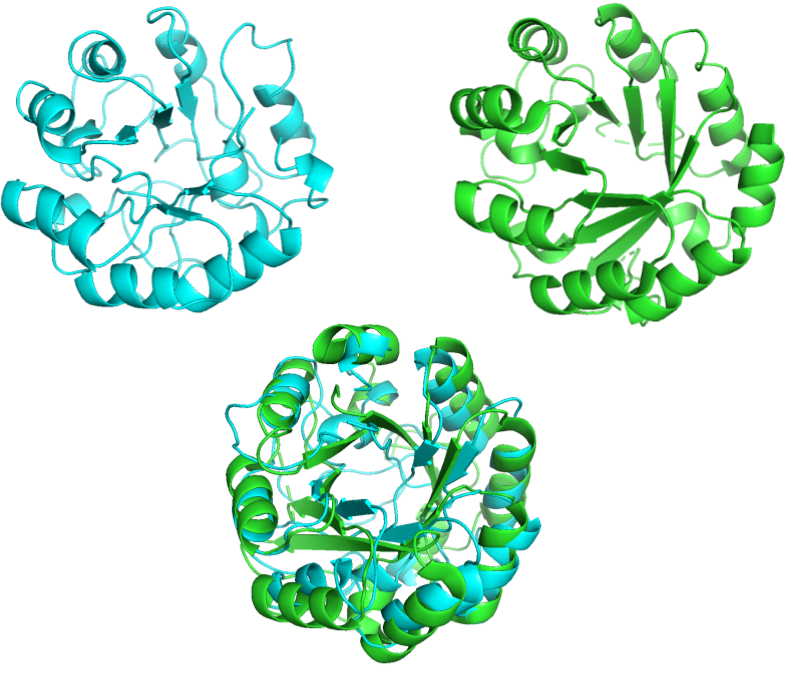
\includegraphics[angle = 0,scale = .5]{chapter4/Couplings/PriACouplingFoldings.png}
  \caption[Superposición de estructura de PriA generado por Folding con la estructura cristalográfica]{\footnotesize{Comparación de estructura tridimensional de PriA generada por EVcouplings con una estructura cristalográfica de {Streptomyces} {coelicolor}. En azul se muestra la estructura generada considerando acoplamientos de los aminoácidos de PriA según el registro evolutivo. En verde está la estructura 1vzw obtenida experimentalmente. En la parte inferior de la figura se muestran las dos estructuras alineadas. Su RMSD es de 3.362 
  {A}}}
  \label{fig:CouplingsFoldingPriA}
  \end{figure}
  
  Finalmente los aminoácidos utilizados en la evolución dirigida de la
  sección anterior fueron comparados con los provistos por EVcouplings
  como altamente partícipes en la covariación. Los 10 amnoácidos con más
  acoplamientos fueron 90L, 117V, 127V, 48W, 208I, 87D, 135T, 21V, 109E.
  El número indica la posición de la secuencia y la letra es el código de
  los aminoácidos. Por ejemplo 87D es la posición 87 el aminoácido ácido
  aspártico. Sólo el 21V es parte los aminoácidos mutados en el estudio
  previament descrito. En la \autoref{tab:aminoacidos} se muestra en la
  primera columna los aminoácidos variados en el estudio de mutación
  dirigida en \emph{Corynebacterium}, en la segunda columna el aminoácido
  correspondiente en la secuencia de \emph{Streptomyces coelicolor} y
  finalmente su correspondiente acoplamiento más significativo.\\
  
  \begin{longtable}[]{@{}ccc@{}}
  \caption{Árboles EvoMining de PriA en MicroReact
  \label{tab:aminoacidos}}\tabularnewline
  \toprule
  \emph{Corynebacterium} & \emph{Streptomyces} & Acoplamiento más
  relevante\tabularnewline
  \midrule
  \endfirsthead
  \toprule
  \emph{Corynebacterium} & \emph{Streptomyces} & Acoplamiento más
  relevante\tabularnewline
  \midrule
  \endhead
  D20V & 21V & 173T\tabularnewline
  L48I & 49L & 76I\tabularnewline
  F50L & 51L & 70V\tabularnewline
  M66I & 67I & 80L\tabularnewline
  T80S & 81S & 102N\tabularnewline
  A97C & 98C & 107A\tabularnewline
  D127A & 128G & 164V\tabularnewline
  A129D & 130D & 168I\tabularnewline
  T139L & 136L & 151T\tabularnewline
  Y214L & 211Y & -\tabularnewline
  E230A & 227A & 234E\tabularnewline
  \bottomrule
  \end{longtable}
  
  Una forma gráfica de ver esta tabla es la \autoref{fig:couplings}. Esta
  figura es simétrica porque los acoplamientos son simétricos. Los puntos
  negros indican acoplamientos entre pares de aminoácidos. Entre más cerca
  de la diagonal hay más acoplamientos porque son residuos cercanos en la
  secuencia lineal de la proteína. En las líneas naranjas muestro cómo el
  aminoácido 21D tiene un acoplamiento con el 173T, que está muy cerca del
  175D que ha sido asociado con la actividad de isomerización de PRA, pero
  no de ProFAR. A futuro, para obtener resultados más precisos sobre la
  covariación de residuos en Actinobacteria, se debe proveer un
  alineamiento exclusivo de Actinobacteria.
  
  Finalmente se investigó también la variación individual de los
  aminoácidos catalíticos D11, D130
  {[}\protect\hyperlink{ref-due_bisubstrate_2011}{149}{]} y D175
  reportados en \emph{Mycobacterium
  tuberculosis}{[}\protect\hyperlink{ref-verduzco-castro_co-occurrence_2016}{46}{]}.
  Estas posiciones corresponden en \emph{S coelicolor} a D11, D131 y D171.
  En este trabajo se econtró que existe un conjunto de secuencias donde
  estos residuos presentan variantes \autoref{fig:Alineamiento}. Los
  homólogos más relevantes de PriA/HisA abordados en este capítulo junto
  con las secuencias seleccionadas divergentes en los residuos mencionados
  fueron alineadas para mostrar la diversidad de las familias PriA/HisA a
  nivel de aminoácidos. Aunque existen variantes de 131D fuera del phylum
  Actinobacteria, como en \emph{Pseudomonas}, Cyanobacteria,
  Enterobacteria, Proteobacteria y Chloroflexi también en Actinobacteria
  se encontraron 159 \emph{Corynebacterium}, 49 \emph{Streptomyces} y 2
  \emph{Actinokineospora} con un residuo diferente al aspártico en la
  posición 131. Están depositados en la base pública NCBI hasta Enero de
  2019, 349 genomas públicos de \emph{Streptomyces} 2019, así pues
  aproximadamente un 14\% tiene una variante en la posición 131. Entre
  estos \emph{Streptomyces} están el ya mencionado \emph{Streptomyces } CT
  34 que posee dos copias de PriA una de ellas muy divergente y el
  \emph{Streptomyces rimosus} del que se habló en en capítulo anterior
  porque sintetiza rimosamidas. Es llamativo que las variantes de 131D se
  encuentran principalmente en \emph{Corynebacterium} y en
  \emph{Streptomyces} que corresponden a los géneros donde se han ubicado
  a la familia subHisA y a la familia PriB respectivamente. La
  variabilidad mostrada en estos géneros podría estar relacionada con la
  existencia de estas familias. Otros los \emph{Streptomyces} con una
  variante en 131D son \emph{S. oceani} , \emph{S. scabiei}, \emph{S.
  fradiae}, \emph{S. rimosus} , \emph{S. sp.} CT34 y \emph{S. } MUSC 14 y
  \emph{S. D11H} . De ellos los tres últimos son además los únicos
  \emph{Streptomyces} con la variante D11H que comparten con
  \emph{Actinokineospora auranticolor}. De hecho las tres posiciones
  conservadas en la mayoría de las PriA presentan variantes en estos
  cuatro organismos, por lo que sería interesante caracterizarlos
  bioquímicamente. Entre los organismos con doble copia de PriA están
  \emph{Serinicoccus marinus} , \emph{Serinicoccus profundi} y
  \emph{Ornithinimicrobium pekingense}, ambas copias fueron incluidas en
  el alineamiento. Estas seis secuencias de PriA tienen aspártico en las
  tres posiciones conservadas, las diferencias que muestran en otras
  posiciones indican que las copias primarias y las secundarias de cada
  organismo se agrupan entre sí. La secuencia de \emph{Actinomadura sp.}
  ATCC 39365 involucrada en el BGC \emph{ada} es similar a la PriA de
  \emph{S. coelicolor} por lo que posiblemente PriA de \emph{S.
  coelicolor} también podría presentar esta actividad. Se incluyó en el
  análisis una secuencia reconstruída del ancestro común de HisA en
  Bacteria {[}\protect\hyperlink{ref-plach_long-term_2016}{33}{]}, esta
  secuencia muestra el aspártico en las tres posiciones. En Cyanobacteria
  la HisA del BGC saxitoxina es prácticamente igual a la de
  \emph{Cylindrospermopsis raciborskii} CS50 y ambas conservan el
  aspártico en las tres posiciones. En Archaea las PriA más grandes
  encontradas \emph{Halorubrum tebenquichense} y \emph{Halonotius sp
  J07HN6} tienen la variante en D171E, que comparten con los
  \emph{Streptomyces} y la \emph{Actinokineospora} con variante D11H y con
  los \emph{Streptomyces} con la variante D130E. Finalmente también en
  Archaea \emph{Thermococcus sp JCM 11816} que comparte el contexto
  genómico con genes de triptofano presenta los tres reiduos conservados.
  
  \begin{figure}[h!tbp]
  \centering
  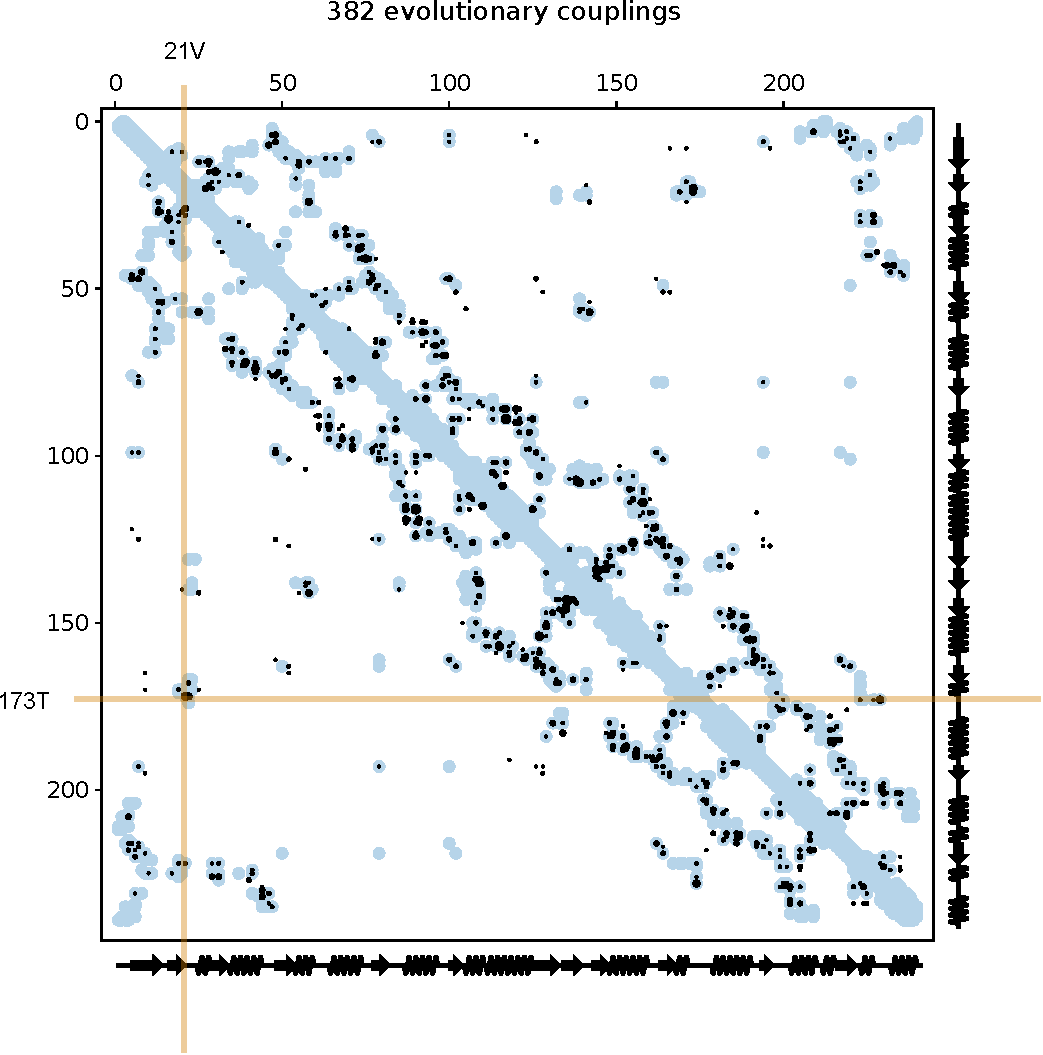
\includegraphics[angle = 0,scale = .5]{chapter4/Couplings/HIS4_STRCO_1-200/align/couplings.pdf}
  \caption[Visualización de los acoplamientos en la familia PriA]{\footnotesize{Visualización de los acoplamientos en la familia PriA}}
  \label{fig:couplings}
  \end{figure}
  
  \begin{figure}[h!tbp]
  \centering
  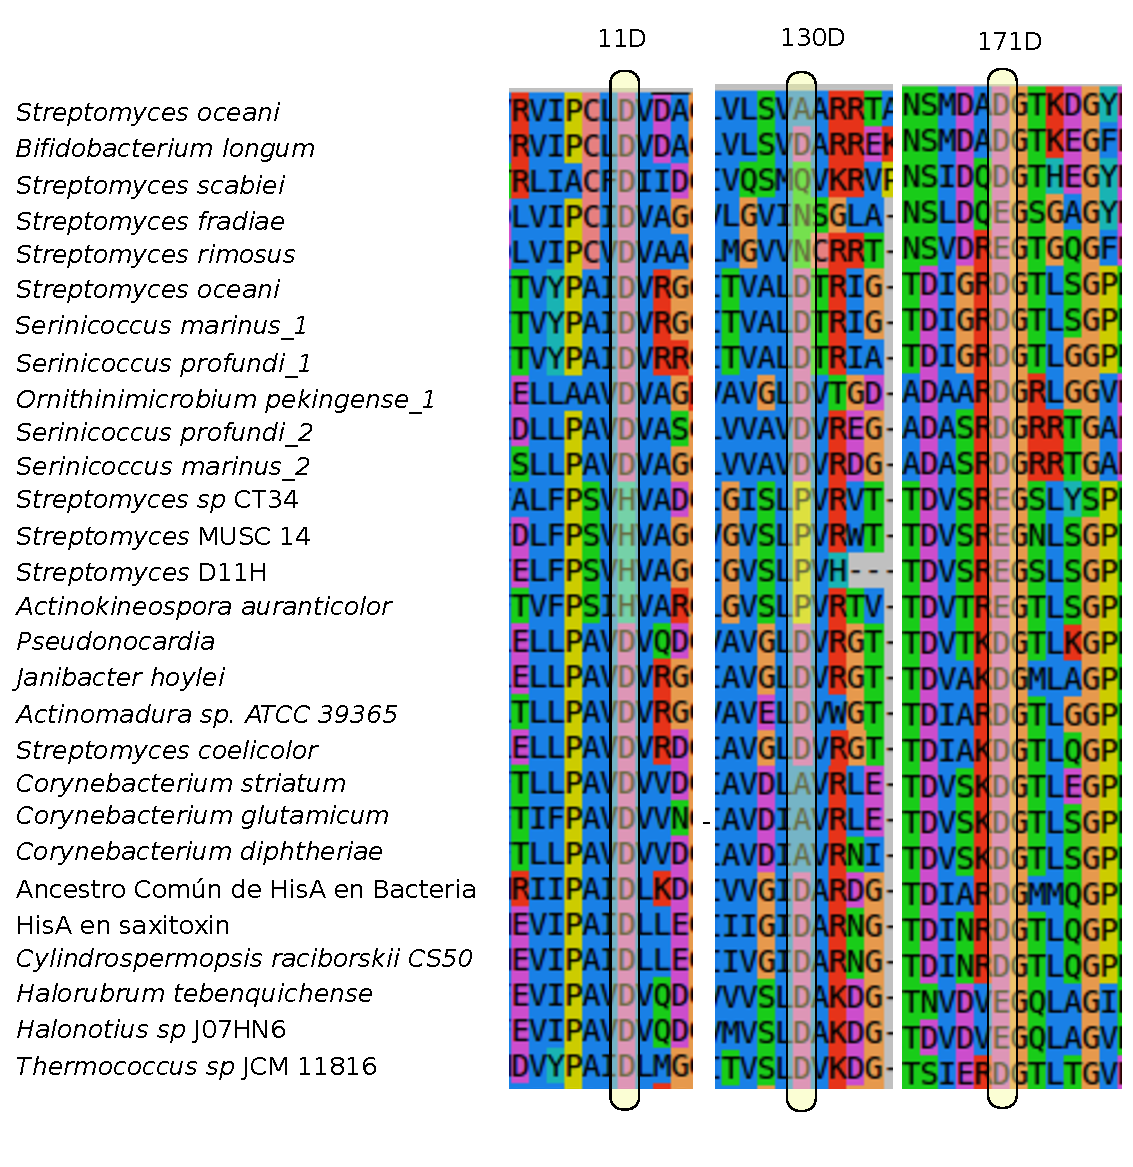
\includegraphics[angle = 0,scale = .8]{chapter4/Couplings/alineamiento.pdf}
  \caption[Miembros de PriA que poseen variantes los residuos catalíticos D11, D130]{\footnotesize{Miembros de PriA que poseen variantes los residuos catalíticos D11, D130}}
  \label{fig:Alineamiento}
  \end{figure}
  
  \clearpage
  
  \section{Afinidad de enzimas selectas por sustratos químicamente
  parecidos a PRA y
  PROFAR}\label{afinidad-de-enzimas-selectas-por-sustratos-quimicamente-parecidos-a-pra-y-profar}
  
  Además de los sustratos conocidos ProFAR y PRA en los que PriA es capaz
  de realizar una isomerización, es posible que PriA pueda ser promiscua
  en otros sustratos. De hecho, como se vio en la sección de EvoMining de
  este capítulo PriA parece participar en la síntesis del antibiótico
  pentostaina ( \emph{ada} BGC). Tomando este ejemplo como inspiración, se
  buscaron sustratos químicamente parecidos a ProFAR y PRA. Esta sección
  buscará probar la afinidad de sustratos parecidos a los nativos de PriA
  para posteriormente probar alguno en copias selectas de PriA
  provenientes de diversos organismos. Veinte sustratos (S1, S2, \ldots{}
  S20) fueron recolectados tanto de la literatura
  {[}\protect\hyperlink{ref-adams_promiscuous_2014}{42}{]} como de
  predicciones quimioinformáticas
  {[}\protect\hyperlink{ref-jeffryes_mines_2015}{151}{]}. Estos sustratos
  son mostrados en \autoref{fig:Eschema1},
  \autoref{fig:Eschema2},\autoref{fig:Eschema3},\autoref{fig:Eschema4}.
  Los sustratos nativos son PRA (S3) y el sustrato PROFAR es S7. Por otra
  parte, S13-S16 son sustratos activados por luz. Los sustratos S17 (PRAP)
  y S18 (Compuesto V) se encontraron en la literatura, mientras que S6
  (GMP), S11 (GTP) y otros fueron sugeridos por el grupo del dr. Chris
  Henry debido a sus similitudes quimioinformáticas. En la siguiente
  sección, posteriormente a la selección de sustratos seleccionaremos las
  secuencias de PriA con las cuales se realizará el docking
  enzima-sustrato.
  
  \begin{figure}[h!tbp]
  \centering
  \includegraphics[angle = 0,scale = .8]{chapter4/SustratosQuimicos.pdf}
  \caption[Substatos químicamente similares a los sustratos de PriA (parte 1)]{\footnotesize{Substatos químicamente similares a los sustratos de PriA (parte 1)}}
  \label{fig:Eschema1}
  \end{figure}
  
  \begin{figure}[h!tbp]
  \centering
  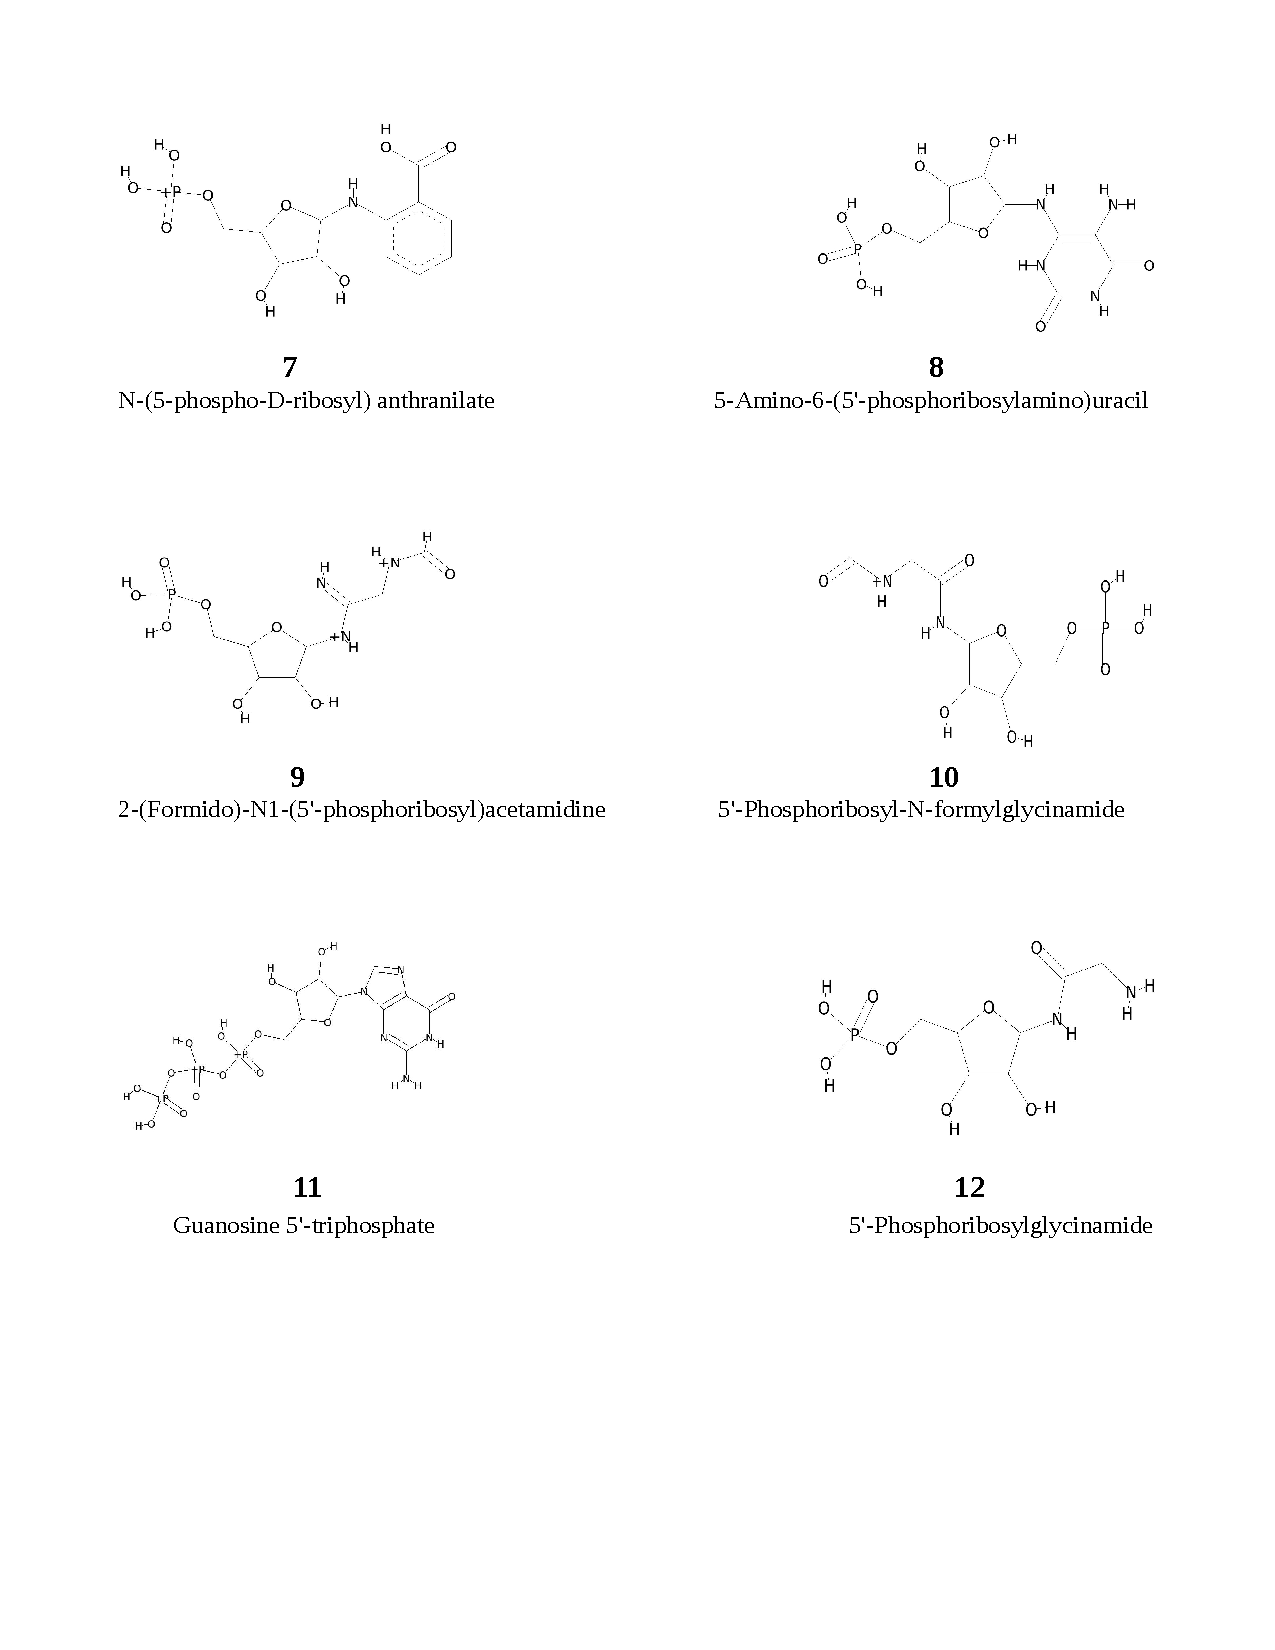
\includegraphics[angle = 0,scale = .8]{chapter4/esquema_quimico-2-2.pdf}
  \caption[Substatos químicamente similares a los sustratos de PriA (parte 2)]{\footnotesize{Substatos químicamente similares a los sustratos de PriA (parte 2)}}
  \label{fig:Eschema2}
  \end{figure}
  
  \begin{figure}[h!tbp]
  \centering
  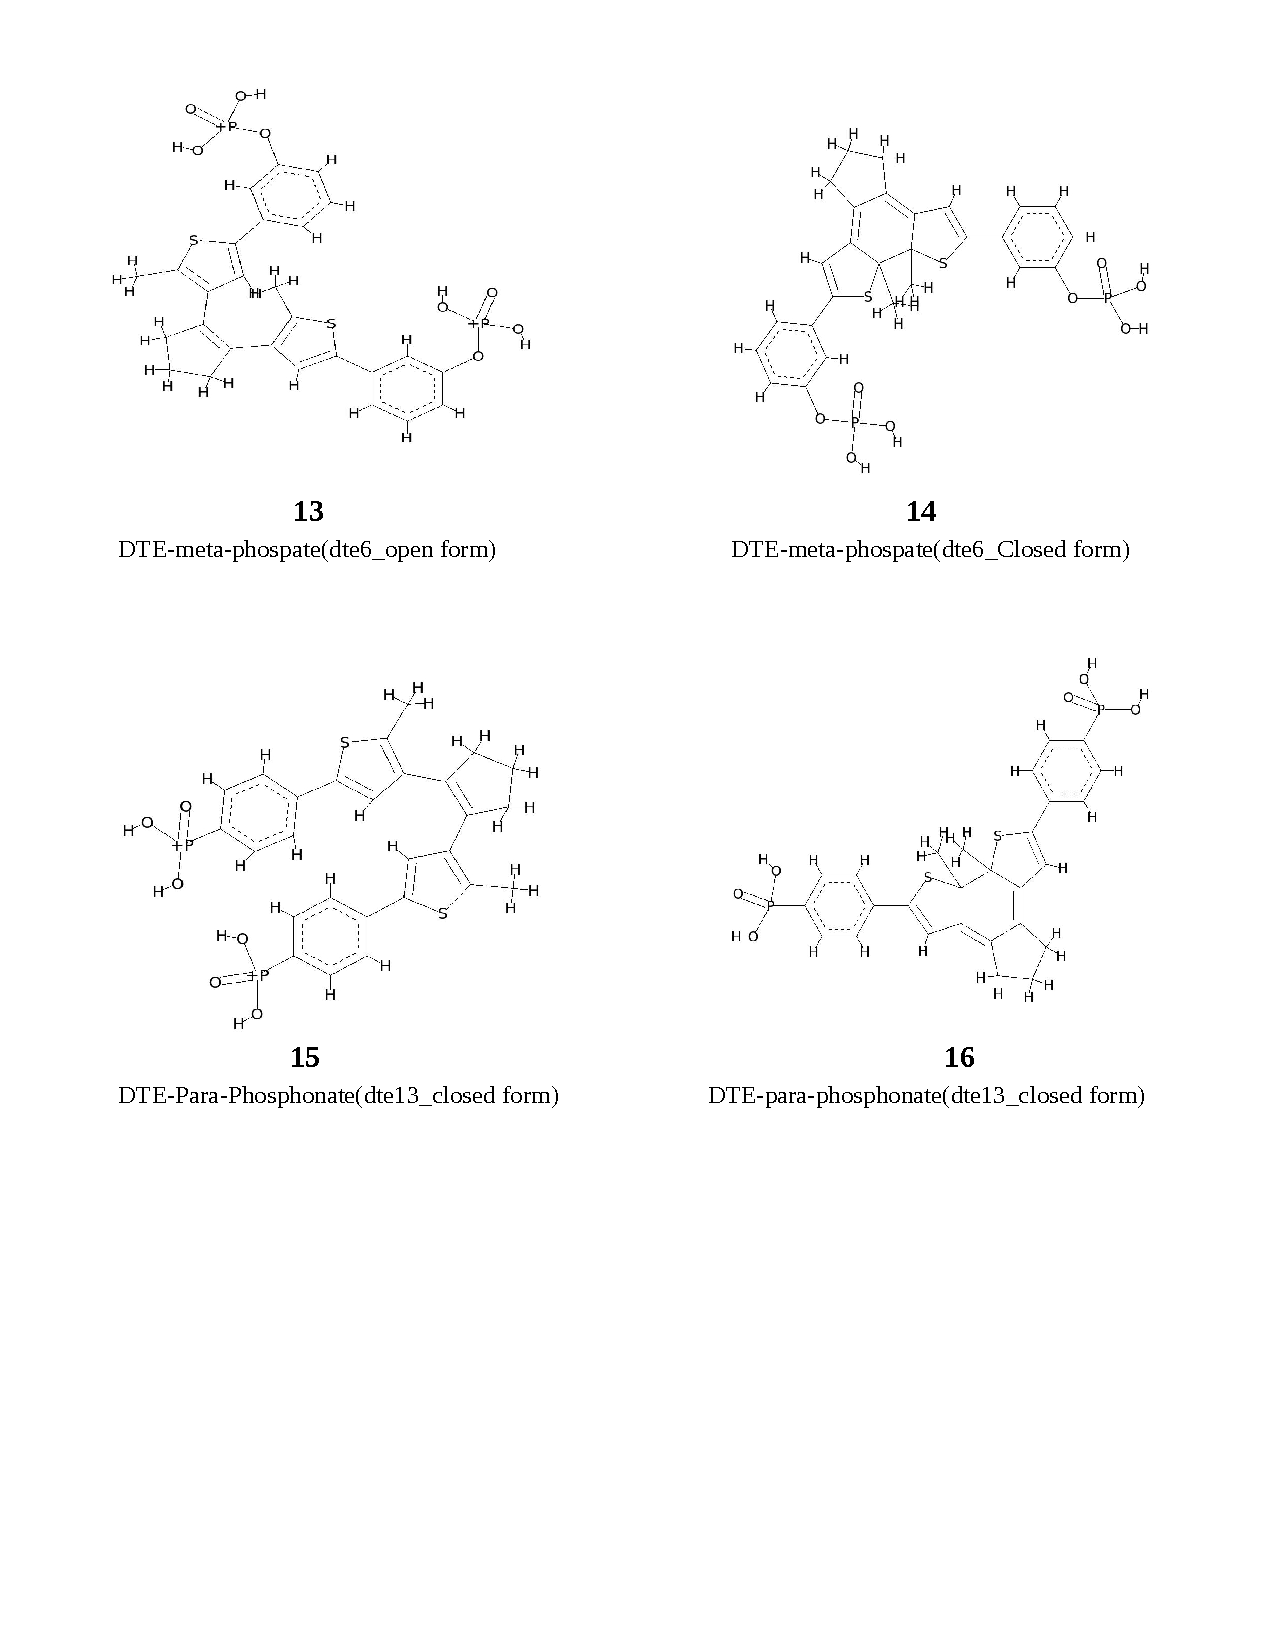
\includegraphics[angle = 0,scale = .8]{chapter4/esquema_quimico-3-3.pdf}
  \caption[Substatos químicamente similares a los sustratos de PriA (parte 3)]{\footnotesize{Substatos químicamente similares a los sustratos de PriA (parte 3)}}
  \label{fig:Eschema3}
  \end{figure}
  
  \begin{figure}[h!tbp]
  \centering
  \includegraphics[angle = 0,scale = .8]{chapter4/esquema_quimico-4-4.pdf}
  \caption[Substatos químicamente similares a los sustratos de PriA (parte 4)]{\footnotesize{Substatos químicamente similares a los sustratos de PriA (parte 4)}}
  \label{fig:Eschema4}
  \end{figure}
  
  \clearpage  
  
  \subsection{Selección de secuencias de PriA o familias relacionadas para
  docking con sustratos similares a lo
  nativos}\label{seleccion-de-secuencias-de-pria-o-familias-relacionadas-para-docking-con-sustratos-similares-a-lo-nativos}
  
  Una vez escogidos los sustratos quedaban por definir las secuencias con
  las que se llevaría a cabo el análisis bioinformático de acoplamiento
  enzima-sustrato, lo que hicimos en colaboración con el grupo del dr.
  Carillo-Trip. Para ello seleccioné 39 secuencias de la familia PriA y
  sus subfamilias, entre ellas incluí varios \emph{Streptomyces} para
  tener tanto secuencias perteneciantes a PriA y como a la subfamilia
  PriB. Estas secuencias seleccionadas de PriA / PriB están uniformemente
  distribuidas en \emph{Streptomyces} de acuerdo a un árbol de especies de
  \emph{Streptomyces} basado en la proteína RpoB. Además estos
  \emph{Streptomyces} tienen variedad en cuanto a la presencia / ausencia
  de \emph{trpF} en su genoma. Se incluyeron además otros homólogos de
  PriA que han sido caracterizados químicamente y finalmente se con el
  mismo criterio de carcaterización bioquímica se agregaron secuencias de
  HisA de \emph{Escherichia coli}, \emph{Arthrobacter Aurescens},
  \emph{Salmonella enterica} y \emph{Acidimicrobium ferrooxidans} y
  secuencias TrpF provenientes \emph{Jonesia denitrificans} y
  \emph{Streptomyces sp } Mg1 para ser utilizadas como controles.
  
  Para realizar el docking se requieren estructuras cristalográficas.
  Cuando existían estructuras cristalográficas de la secuencia específica
  de PriA del organismo se utilizó dicha estructura. En caso contrario, el
  grupo del Dr Carrillo-Tripp generó estructuras homólogas utilizando la
  técnica de modelado por homología mediante el software Rosseta. Para
  cada secuencia decidí usar como plantilla la estructura tridimensional
  del homólogo de PriA más cercano que sí contara estructura con
  estructura cristalográfica. Los organismos con estructura
  cristalográfica de alguna familia relacionada a PriA están descritos en
  la \autoref{tab:EnzymePDB}. Para este análisis fueron las secuencias con
  estructura(s) cristalográfica(s) seleccionadas fueron: para la familia
  HisA la Enterobacteria \emph{Salmonella enterica} (PDB:5AHE), para la
  familia subHisA la Actinobacteria \emph{Actinomyces urogenitalis}
  (PDB:4X2R), la estructura que representa a subTrpF es la de
  \emph{Arthrobacter aurescens} (PDB:4WD0). En cuanto a la familia PriA,
  varias estructuras cristalográficas de \emph{Mycobacterium tuberculosis}
  (Mtub PDB:2Y88,2Y89,2Y85,3ZS4) y \emph{Streptomyces coelicolor} (Scoe
  PDB:2VEP,2X30,1VZW) fueron incluidas. Las estructuras de PriB
  consideradas fueron las de \emph{Streptomyces sviceus} (PDB:4U28,4TX9) y
  las de \emph{Streptomyces sp} Mg1 (4W9T, 4X9S). Finalmente la estructura
  cristalográfica de TrpF corresponde a \emph{Jonesia denitrificans}
  (PDB:4WUI). \autoref{tab:EnzymeDocking}.
  
  Se incluyeron también enzimas TrpF provenientes de \emph{Streptomyces
  Mg1, Jonesia denitrificans}. Las estructuras cristalográficas
  disponibles de PriB provienen de de . . \emph{Streptomyces globisporus},
  \emph{Actynomyces urogenitalis} (4X2R) y \emph{Corynebacterium jeikeum}.
  De la familia subHisA se muestran \emph{Corynebacterium efficiens} y . y
  finalmente, \emph{Chlamidya thrachomatis}, \emph{Streptomyces sp. Mg1} y
  \emph{Actinomyces odontolyticus}. Las representantes de la familia TrpF
  son las Actinobacterias \emph{Jonesia denitrificans} y
  \emph{Streptomyces sp Mg1}. A continuación se muestra una tabla con las
  estructuras cristalográficas disponibles de PriA y familias
  relacionadas.
  
  \begin{longtable}[]{@{}ll@{}}
  \caption{Secuencias selectas de PriA y familias relacionadas para el
  análisis de docking \label{tab:EnzymeDocking}}\tabularnewline
  \toprule
  Abreviatura & Organismo\tabularnewline
  \midrule
  \endfirsthead
  \toprule
  Abreviatura & Organismo\tabularnewline
  \midrule
  \endhead
  Save & \emph{Streptomyces avellaneus}\tabularnewline
  Scar & \emph{Streptomyces carneus}\tabularnewline
  Spur & \emph{Streptomyces purpeofuscus}\tabularnewline
  Smeg & \emph{Streptomyces megasporus}\tabularnewline
  Sfrad & \emph{Streptomyces fradiae}\tabularnewline
  Svar & \emph{Streptomyces varsoviensis}\tabularnewline
  Satra & \emph{Streptomyces atratus}\tabularnewline
  Srim & \emph{Streptomyces rimosus} R6-500\tabularnewline
  SCT34 & \emph{Streptomyces sp.} CT34\tabularnewline
  S1813 & \emph{Streptomyces sp.} NRRL S-1813\tabularnewline
  Ssul & \emph{Streptomyces sulphureus} DSM 40104\tabularnewline
  Scla & \emph{Streptomyces clavuligerus} ATCC 27064\tabularnewline
  Stsu & \emph{Streptomyces tsukubaensis} NRRL18488\tabularnewline
  Sbik & \emph{Streptomyces bikiniensis}\tabularnewline
  Sven & \emph{Streptomyces venezuelae} ATCC 10712\tabularnewline
  Sful & \emph{Streptomyces fulvoviridis}\tabularnewline
  Scal & \emph{Streptomyces californicus}\tabularnewline
  Sbaa & \emph{Streptomyces baarnensis}\tabularnewline
  Salb & \emph{Streptomyces albus} J1074\tabularnewline
  Siak & \emph{Streptomyces iakyrus}\tabularnewline
  Sgha & \emph{Streptomyces ghanaensis} ATCC 14672\tabularnewline
  Sbic & \emph{Streptomyces bicolor}\tabularnewline
  Sipo & \emph{Streptomyces ipomoeae} 91-03\tabularnewline
  Sbot & \emph{Streptomyces bottropensis} ATCC 25435\tabularnewline
  SspC & \emph{Streptomyces sp.} C\tabularnewline
  SMg1 & \emph{Streptomyces sp.} Mg1\tabularnewline
  Sxan & \emph{Streptomyces xanthophaeus}\tabularnewline
  Skat & \emph{Streptomyces katrae}\tabularnewline
  Slav & \emph{Streptomyces lavendulae subsp. lavendulae}\tabularnewline
  Sery & \emph{Streptomyces erythrochromogenes}\tabularnewline
  Sniv & \emph{Streptomyces niveus} NCIMB 11891\tabularnewline
  Ssvi & \emph{Streptomyces sviceus} ATCC 29083\tabularnewline
  Sfla & \emph{Streptomyces flaveus}\tabularnewline
  Save & \emph{Streptomyces avermitilis} MA-4680 = NBRC
  14893\tabularnewline
  Scoe & \emph{Streptomyces coelicolor} A3(2)\tabularnewline
  ArTC1 & \emph{Arthrobacter aurescens} TC1\tabularnewline
  Sglob & \emph{Streptomyces globisporus} C-1027\tabularnewline
  Sgri & \emph{Streptomyces griseolus}\tabularnewline
  S34 & \emph{Streptomyces sp. } CT34 (paralogo)\tabularnewline
  \bottomrule
  \end{longtable}
  
  \begin{longtable}[]{@{}ccccc@{}}
  \caption{Estructuras cristalográficas disponibles de PriA y familias
  relacionadas \label{tab:EnzymePDB}}\tabularnewline
  \toprule
  Organismo & PDB & Familia & Resolución \({\AA}\) & Fecha\tabularnewline
  \midrule
  \endfirsthead
  \toprule
  Organismo & PDB & Familia & Resolución \({\AA}\) & Fecha\tabularnewline
  \midrule
  \endhead
  \emph{Salmonella enterica} & 5AHE & HisA & 1.7 & 2015\tabularnewline
  \emph{Salmonella enterica} & 5AB3 & HisA & 1.8 & 2016\tabularnewline
  \emph{Salmonella enterica} & 5ABT & HisA & 1.65 & 2016\tabularnewline
  \emph{Salmonella enterica} & 5AC7 & HisA & 1.9 & 2016\tabularnewline
  \emph{Salmonella enterica} & 5AC8 & HisA & 1.7 & 2016\tabularnewline
  \emph{Salmonella enterica} & 5AC6 & HisA & 1.99 & 2016\tabularnewline
  \emph{Salmonella enterica} & 5A5W & HisA & 1.6 & 2015\tabularnewline
  \emph{Salmonella enterica} & 5AHF & HisA & 2.2 & 2012\tabularnewline
  \emph{Thermotoga maritima} & 2W79 & HisA & 1.85 & 2008\tabularnewline
  \emph{Thermotoga maritima} & 1QO2 & HisA & 1.85 & 2000\tabularnewline
  \emph{Streptomyces sp.} Mg1 & 4X9S & PriB & 1.6 & 2014\tabularnewline
  \emph{Streptomyces sviceus} & 4TX9 & PriB & 1.6 & 2014\tabularnewline
  \emph{Streptomyces sviceus} & 4U28 & PriB & 1.33 & 2014\tabularnewline
  \emph{Streptomyces sp.} Mg1 & 4W9T & PriB & 1.57 & 2014\tabularnewline
  \emph{Arthrobacter aurescens} & 4WD0 & subTrpF & 1.5 &
  2014\tabularnewline
  \emph{Streptomyces coelicolor} & 5DN1 & PriA & 1.95 &
  2015\tabularnewline
  \emph{Streptomyces coelicolor} & 1VZW & PriA & 1.8 & 2004\tabularnewline
  \emph{Streptomyces coelicolor} & 2VEP & PriA & 1.8 & 2007\tabularnewline
  \emph{Streptomyces coelicolor} & 2X30 & PriA & 1.95 &
  2010\tabularnewline
  \emph{Mycobacterium tuberculosis} & 2Y85 & PriA & 2.4 &
  2011\tabularnewline
  \emph{Mycobacterium tuberculosis} & 2Y88 & PriA & 1.33 &
  2011\tabularnewline
  \emph{Mycobacterium tuberculosis} & 2Y89 & PriA & 2.5 &
  2011\tabularnewline
  \emph{Mycobacterium tuberculosis} & 3ZS4 & PriA & 1.9 &
  2012\tabularnewline
  \emph{Actinomyces urogenitalis} & 4X2R & SubHisA & 1.05 &
  2014\tabularnewline
  \emph{Corynebacterium efficiens} & 4AXK & SubHisA & 2.25 &
  2013\tabularnewline
  \emph{Thermococcus kodakaraensis} & 5LHE & TrpF & 1.85 &
  2016\tabularnewline
  \emph{Thermococcus kodakaraensis} & 5LHF & TrpF & 1.75 &
  2016\tabularnewline
  \emph{Thermus thermophilus} & 1V5X & TrpF & 2 & 2003\tabularnewline
  \emph{Thermotoga maritima} & 1DL3 & TrpF & 2.7 & 1999\tabularnewline
  \emph{Thermotoga maritima} & 1LBM & TrpF & 2.8 & 2002\tabularnewline
  \emph{Thermotoga maritima} & 1NSJ & TrpF & 2 & 1996\tabularnewline
  \emph{Jonesia denitrificans} & 4WUI & TrpF & 1.09 & 2014\tabularnewline
  \emph{Pyrococcus furiosus} & 4AAJ & TrpF & 1.75 & 2012\tabularnewline
  \bottomrule
  \end{longtable}
  
  \subsection{El análisis de PriA a nivel estructural sugiere que GTP es
  el sustrato más
  afín}\label{el-analisis-de-pria-a-nivel-estructural-sugiere-que-gtp-es-el-sustrato-mas-afin}
  
  Con las estructuras de las enzimas seleccionadas de PriA se realizaron
  simulaciones de docking respecto a los veinte sustratos descritos. El
  procedimiento puede ser consultado en
  \href{https://github.com/tripplab/Docking/wiki}{Docking Protocols}. En
  la \autoref{fig:HeatplodPriAdocking} presento una visualización de los
  resultados obtenidos. En esta figura se marcan en color los organismos
  de los que se tiene una caracterización bioquímica, en azul están las
  secuencias correspondientes a TrpF, en rojo las de HisA, en rosa las
  secuencias de PriA y subHisA y en verde las de PriB y subTrpF. Con un
  asterisco fueron marcadas las secuencias de las que se cuenta con
  estructura cristalográfica. En el caso de las secuencias que no contaban
  con estructura cristalográfica, la estructura que sirvió como base está
  anotada después de la abreviatura del organismo. Las abreviaturas
  corresponden a los organismos de la \autoref{tab:EnzymeDocking}. Los
  cuadrados grises son datos que faltaron de simular. Entre más azul es
  mayor la afinidad del sustrato por la secuencia, entre más rojo menor la
  afinidad de la enzima por este sustrato. Se requieren más controles para
  este experimento, pero una tendencia general es que la columna
  correspondiente a S11 (GTP) es el sustrato que tiene mayor afinidad. Por
  ello, aunque afinidad no tiene porque corresponder con capacidad
  catalítica, se decidió investigar la capacidad de secuencias de PriA
  para catalizar alguna reacción sobre el GTP, esa investigación es el
  objeto de la última sección de este capítulo.
  
  \begin{figure}[h!tbp]
  \centering
  \includegraphics[angle = 0,scale = .7]{chapter4/Figura1_4.pdf}
  \caption[Heatplot del docking de enzimas relacionadas a PriA vs posibles substratos]{\footnotesize{Heatplot del docking de enzimas relacionadas a PriA vs posibles substratos}}
  \label{fig:HeatplodPriAdocking}
  \end{figure}
  
  \clearpage
  
  \section{PriA en cinéticas enzimáticas no
  tradicionales.}\label{pria-en-cineticas-enzimaticas-no-tradicionales.}
  
  Después de la exploración genómica de PriA/HisA se trabajó en
  caracterizaciones experimentales no tradicionales de PriA. No se tuvo el
  tiempo ni la experiencia para tener réplicas de los resultados descritos
  a continuación, sin embargo se incluyen en esta tesis porque pueden ser
  un buen comienzo para luego retomar este trabajo. Los protocolos fueron
  cuidadosamente descritos y se encuentran incluidos en los anexos. Este
  capítulo se enfoca en el montaje de dos experimentos, el primero
  sugerido por la sección anterior: \emph{i)} Cinéticas de PriA en GTP.
  Mientras que el segundo está motivado por la curiosidad sobre el cambio
  en la capacidad catalítica según se provea primero un sustrato u otro,
  este experimento consiste en la \emph{ii)} Medición simultánea de la
  actividad de PriA sobre ProFAR y PRA.
  
  Lo primero que se realizó fue la sobre-expresión heteróloga de PriA. La
  secuencia de PriA fue clonada en cepas de \emph{E. coli} V68 donde se
  indujo la sobre expresión. A partir de este cultivo productor de PriA se
  purificó la proteína. Se corroboró el éxito de esta actividad mediante
  un gel de proteína en la que puede verse expresión en la barra
  correspondiente al tamaño de PriA \autoref{fig:gel}. La proteína
  purificada fue almacenada a -80° en esferas de proteína selladas con
  nitrógeno líquido para su mejor preservación, tal y como se describe en
  el anexo de los procedimientos. Con este \emph{stock} de proteína se
  realizaron cinéticas enzimáticas \emph{in vitro}.
  
  \begin{figure}[h!tbp]
  \centering
  \includegraphics[angle = 0,scale = 0.6]{chapter4/Geles/PriAAbril30.png}
  \caption[gel]{\footnotesize{Gel de proteína donde se muestra la banda correspondiente a PriA después de ser sobre-expresada y purificada}}
  \label{fig:gel}
  \end{figure}
  
  \subsection{PriA puede metabolizar
  GTP}\label{pria-puede-metabolizar-gtp}
  
  Como se sugirió en la sección anterior PriA puede tener actividad sobre
  GTP. Ahora bien, la actividad de PriA en ProFAR es medida en un ensayo
  estandarizado mediante la detección de cambio de fluorescencia. Para
  esta medición por fluorimetría se coloca la enzima en placas de 96 pozos
  (Nuc 96-Well Optical Botto Plates), se agrega el sustrato y utilizando
  un lector de fluorescencia de placas (TECAN infinite M1000) se mide el
  cambio de fluorescencia en el tiempo. Una variación de este ensayo
  permitió obtener información sobre la actividd PriA sobre dGTP. Los
  parámetros utilizados para la medición fueron tomados del trabajo no
  publicado de Verduzco-Castro en este laboratorio (exitación a 255 nm y
  emisión a 334 nm). Para comenzar esta investigación se utilizó primero
  dGTP en lugar de GTP esto debido a que el dGTP es un sustrato siempre
  disponible en cualquier laboratorio ya que es necesario para la reacción
  de PCR. Así pues, ensayos preliminares de actividad de PriA sobre este
  dGTP se realizaron en la proteína purificada de PriA de
  \emph{Streptomyces coelicolor}, activa en ambos sustratos nativos
  utilizando como control su mutante inactiva que sustituye en la posición
  11 el ácido aspártico por una alanina (D11A). La
  \autoref{fig:PriAActividaddGTP} muestra el resultado de este experimento
  donde se aprecia un decrecimiento mayor en la fluorescencia del pozo que
  contiene la proteína activa respecto del pozo que contiene a la mutante.
  
  \begin{figure}[h!tbp]
  \centering
  \includegraphics[angle = 0,scale = 0.8]{chapter4/MutantControl.png}
  \caption[PriA de {S.}{coelicolor} y su mutante no funcional sobre dGTP]{\footnotesize{PriA de {S.}{coelicolor} y su mutante no funcional sobre dGTP}}
  \label{fig:PriAActividaddGTP}
  \end{figure}
  
  Este experimento de detección de actividad de dGTP fue ampliado
  incluyendo ahora proteínas provenientes de otros organismos. Para ello
  se utilizaron los stocks disponibles de PriA provenientes de
  \emph{Streptomyces roseus} , \emph{Thermomonospora curvata} y
  \emph{Mycobacterium smegmatis}; los stocks de PriB provenientes de
  \emph{Streptomyces sp C}, \emph{Streptomyces sviceus} y de
  \emph{Streptomyces sp} Mg1 y finalmente el stocks de TrpF de
  \emph{Jonesia denitrificans}. El ensayo descrito arriba fue realizado en
  estas enzimas y el resultado es mostrado en
  \autoref{fig:dGTPActividadHomologos}. En la parte inferior derecha vemos
  que como debe ser el control negativo, el pozo con Buffer y sustrato no
  muestra ningún cambio en la fluorescencia. Sin embargo no es claro que
  exista una tendencia claramente decreciente en los pozos que contienen
  enzima. Posiblemente la pendiente que se observa en los datos de
  \emph{Thermomonospora curvata}, indique cierta actividad sobre dGTP.
  Este comportamiento también puede deberse a que las proteínas llevaban
  tiempo almacenadas. Los experimentos deben ser repetidos con proteína
  recién purificada.
  
  \begin{figure}[h!tbp]
  \centering
  \includegraphics[angle = 0,scale = 0.6]{chapter4/GTPCinetica.png}
  \caption[Homólogos de PriA y familias relacionadas no muestran actividad clara sobre dGTP]{\footnotesize{Actividad de PriA y familias relacionadas de distintos organismos sobre dGTP. Este experimento no muestra disminución de fluorescencia en las enzimas seleccionadas lo que implicaría que no existe actividad importante sobre dGTP, excepto poiblemente en el caso de {Thermomonospora} {curvata}}}
  \label{fig:dGTPActividadHomologos}
  \end{figure}
  
  Finalmente se probó con los mismos parámetros la actividad de PriA de
  \emph{Streptomyces coelicolor} sobre GTP. Se comprobó que la enzima
  estuviera activa mediante ensayos enzimáticos exitosos en sus otros dos
  sustratos. Sin embargo, no se pudo detectar cambio en la fluorescencia
  de GTP debido a la actividad de PriA. Es posible que la PriA de \emph{S
  coelicolor} no pueda catalizar ninguna reacción sobre el GTP por lo que
  una variante que a futuro podría aportar a este experimento es utilizar
  \href{https://www.jenabioscience.com/nucleotides-nucleosides/nucleotides-by-structure/fluorescent-nucleotides/guanosines-intrinsically-fluorescent}{análogos
  fluorescentes de GTP}.
  
  \begin{figure}[h!tbp]
  \centering
  \includegraphics[angle = 0,scale = 0.6]{chapter4/GTP.png}
  \caption[PriA no mostró actividad sobre GTP a diversas concentraciones]{\footnotesize{PriA no mostró actividad sobre GTP. El ensayo enzimático de PriA de {Streptomyces}{coelicolor} sobre GTP a distintas concentraciones no mostró cambios en la fluorescencia de GTP.}}
  \label{fig:GTP}
  \end{figure}
  
  \clearpage 
  
  \subsection{Cinéticas simultáneas para PRA y
  ProFAR}\label{cineticas-simultaneas-para-pra-y-profar}
  
  Otra pregunta que me surgió al investigar la promiscuidad enzimática es
  si esta es una propiedad de la población o de cada una de las enzimas
  existentes en la célula. En PriA esta pregunta puede traducirse a ¿cómo
  saber si cada molécula de PriA cataliza PRA y ProFAR \emph{in vivo}? o
  si en cambio, existe una subpoblación que cataliza la isomerización de
  PRA y otra subpoblación de moléculas que cataliza isomerización de
  ProFAR. Una buena aproximación \emph{in vitro} a este problema sería
  poder medir el comportamiento de una sola molécula en un medio con ambos
  sustratos. Una serie de estos experimentos mostraría si existen
  subpoblaciones dedicadas a la catálisis de uno u otro substrato, o bien
  si todas las enzimas de una población son igualmente promiscuas. La
  existencia de subpoblaciones podría deberse a interacciones de la enzima
  con el sustrato, como por ejemplo que agregar PRA primero al medio
  sesgue el comportamiento de la enzima y la haga mejor para catalizar PRA
  que ProFAR o visceversa.
  
  Para empezar a abordar este problema quisimos medir la actividad de una
  población de PriA sobre PRA y ProFAR. or separado, ambos ensayos están
  montados, pero nunca se ha intentado un ensayo simultáneo. Las
  constantes cataliticas de PriA para la isomerización de ProFAR se mide
  utilizando absorbancia mientras que el ensayo enzimático de
  isomerización de PRA se realiza mediante la medición de fluorescencia.
  En esta sección se empezó a desarrollar un método para medir
  simultáneamente las actividades de Pra y ProFAR. Primero intentamos
  medir ambas actividades secuencialmente pero monitorieando que la señal
  de la otra actividad no se viera afectada. Para esto agregamos la enzima
  entre los segundos 100 y 400 en los pozos que ya tienen todo para que se
  lleve a cabo la catálisis de PRA y observamos cómo la fluorescencia baja
  a todas las concentraciones mientras que la absorbancia se mantiene casi
  constante (FIGURA-N). Luego cerca del segundo 1500 agregué el sustrato
  ProFAR y se observa que la absorbancia cae mientras que la fluorescencia
  en los mismos pozos permanece casi constante. El siguiente paso fue
  medir simultáneamente la actividad de una población de PriA sobre PRA y
  ProFAR y aunque si lo medimos no pudimos optimizarlo lo suficiente para
  medir las constantes catalíticas (datos no mostrados). Las prubas piloto
  sugieren que es posible cuantificar la catálisis de ProFAR y PRA
  simultáneamente y en el caso de los homólogos que también toman a GTP se
  podrían medir incluso las tres actividades catalíticas para identificar
  si hay interacciones entre los sustratos.
  
  \begin{figure}[h!tbp]
  \centering
  \includegraphics[angle = 0,scale = 0.6]{chapter4/Conjunto.png}
  \caption[Se pueden medir las dos actividades de PriA simultáneamente.]{\footnotesize{Se pueden medir las dos actividades de PriA simultáneamente. Se midió secuencialmente la actividad de ProFAR isomerasa y de PRA isomerasa en la misma población de enzimas PriA. Se cuantificó la absorbancia (arriba) y la fluorescencia (abajo) durante casi 3000 segundos. entre los segundos 100 y 400 se agregó la enzima a un buffer que ya tenía PRA y al segundo 1400 se agregó el sustrato ProFAR a la misma preparación. }}
  \label{fig:Conjunto}
  \end{figure}
  
  En este capítulo estudiamos la familia PriA en varios niveles tanto su
  variación enzimática como la variación del contexto genómico. Vimos que
  PriA no habría sido sugerida por EvoMining como una familia promiscua ya
  que no tiene una marca de expansión por número de copias, y sin embargo
  sí es promiscua en Actinobacteria. EvoMining nos proporcionó en
  Cyanobacteria y Archaea un ejemplo donde recupera la historia de HisF
  como expansión ancestral de HisA, mostrando que no todas las expansiones
  van al metabolismo secundario, algunas expansiones son reclutadas por el
  metabolismo conservado. Sin embargo vale la pena reflexionar que en su
  momento HisF fue metabolismo especializado, ya que sólo los organismos
  con la expansión de PriA poseían esta copia que posteriormente fue
  fijada por la evolución. De esta forma tenemos un caso donde es el
  metabolismo ``secundario'' el que alimenta al metabolismo conservado.
  Otras estrategias deben abordarse para identificar familias promiscuas
  donde no sea claro un proceso de expansión. Finalmente encontramos las
  variantes más interesantes de PriA en los linajes seleccionados y
  analizamos residuos importantes de cada una de ellas. Finalmente se
  intentó caracterizar tanto nuevas actividades para PriA como la medición
  simultánea de las actividades nativas, aunque se avanzó en este camino,
  estos experimentos deben ser replicados para mayor validez.
  
  \chapter*{Perspectivas}\label{perspectivas}
  \addcontentsline{toc}{chapter}{Perspectivas}
  
  \setcounter{chapter}{4} \setcounter{section}{0} La promiscuidad ha
  redefinido cómo entendemos la función enzimática. Se ha transitado de
  considerar a todas las enzimas como altamente especialistas a entender
  que muchas de ellas pueden llevar a cabo más de una función metabólica.
  La promiscuidad parece parte del proceso evolutivo, provee material para
  que una posterior duplicación conlleve a la formación de nuevas familias
  enzimáticas. En este trabajo traté de entender la promiscuidad a
  diferentes escalas. Primero diferencié entre la existencia de familias
  promiscuas y la de ortólogos promiscuos miembros de dichas familias.
  Ahora bien, las enzimas suelen formar parte de clusters biosintéticos
  productores de metabolitos. Por ello generalicé el concepto de
  promiscuidad enzimática al de promiscuidad de una familia de BGC, es
  decir consideré ahora a una familia de BGC como una unidad de síntesis y
  me pregunté si podía ser promiscua en el sentido de que variantes del
  BGC, ya sea en la secuencia de los genes del core o en el contenido de
  genes accesorios, produjeran variantes del metabolito. Es decir me
  pregunte si un cluster podría tener promiscuidad por producto. Con estos
  tres niveles en mente: enzima, familia enzimática, y cluster
  biosintético desarrollé Orthocore, EvoMining y CORASON, tres
  herramientas de genómica comparativa con el objetivo de entender mejor
  la promiscuidad enzimática en los niveles descritos.
  
  Con Orthocore pude resolver la filogenia del orden
  \emph{Actinomycetales} utilizando los genes del \emph{core conservado} y
  esto permitió entender que en dicho orden los patrones de especiación
  están relacionados con la pérdida y ganancia de promiscuidad de la
  familia PriA. Además pude utilizar Orthocore para encontrar genes
  marcadores de la especie \emph{Clavibacter michiganensis} que permiten
  diagnosticar la presencia de esta especie en plantas de tomate. Una
  lección de este capítulo es que el \emph{core genome} no sólo contiene
  genes del core metabólico, también puede contener genes productores de
  metabolitos especializados, y este contenido incrementará entre más
  cercanos sean filogenéticamente los organismos del linaje seleccionado.
  Una vez desarrollado Orthocore quedaban por investigar las familias
  enzimáticas contrarias al \emph{core conservado} es decir aquellas que
  sí tienen marcas de cambio en el número de copias de su gen codificante
  en al menos algunos organismos de un linaje genómico. El cambio ya podía
  ser observado porque aplicando Orthocore pueden organizarse
  filogenéticamente organismos de genomas cercanos, por ejemplo los del
  género \emph{Streptomyces}.
  
  Así pues para estudiar no sólo los patrones de expansión sino también
  los de neofuncionalización, en particular los de reclutamiento a
  metabolismo especializado desarrolle a continuación la herramienta
  EvoMining. Las familias señaladas por EvoMining como expandidas y
  reclutadas son candidatos a ser familias promiscuas, y los miembros
  intermedios entre ortólogos dedicados a la función primaria y ortólogos
  dedicados al metabolismo especializado son candidatos, aunque no
  exclusivos a ser miembros promiscuos de la familia. En esta sección
  entendí que las familias del \emph{shell genome} también tienen
  reclutamientos y expansiones, que este comportamiento no es exclusivo de
  ciertas familias del \emph{core genome}. Después de esta observación
  queda pendiente realizar un estudio con todas las enzimas del
  \emph{shell genome} de un linaje para entender cómo son las tendencias
  generales por ejemplo por subsistema metabólico. Con EvoMining
  desarrollé dos ejemplos donde en efecto enzimas de metabolismo
  conservado ( \emph{shell o core} ) mostraban miembros reclutados en el
  metabolismo especializado. El primer ejemplo fueron familias del cluster
  de síntesis de escitonemina en Cyanobacteria. A la fecha este BGC no ha
  sido predicho por otros métodos bioinformáticos ya que está compuesto
  exclusivamente por familias que provienen de expansiones del metabolismo
  primario y no posee ninguna enzima catalogada como exclusivamente
  dedicada al metabolismo especializado. El segundo ejemplo es la familia
  TauD común en los BGC de Rimodamide y Detoxin. Este ejemplo tiene
  expansiones y reclutamientos tanto en Actinobacteria como en
  \emph{Pseudomonas}. El estudio de las variantes de estos BGC fue
  resuelto con el desarrollo de CORASON, una herramienta especializada en
  identificar variantes de contextos genómicos.
  
  Así pues desarrollé CORASON para ver el continuo de variantes de un BGC
  en un linaje genómico. Con esta herramienta, al observar la amplia
  variación en cuanto a presencia y ausencia de genes accesorios en
  Actinobacteria de la familia rimosamide-detoxin BGC pensé que esta
  familia de clusters debía ser promiscua. Además esta observación estaba
  soportada por el hecho de que rimosamide y detoxin compartían un core
  molecular común posiblemente relacionado con el core génico de la
  familia, pero tenían las moléculas se diferenciaban en ciertos
  ornamentos, probablemente debidos a los genes accesorios de la familia.
  Propuse pues que esta familia de BGC es promiscua, y que al seleccionar
  genomas de diversos clados del árbol del BGC se deberían encontrar
  nuevas variantes moleculares. Exitosamente,nuestro grupo de
  colaboradores pudo caracterizar dos nuevas variantes al core molecular
  rimosamide - detoxin comprobando así la amplia promiscuidad de esta
  familia.
  
  En este punto quedó pendiente tener una medida de la diversidad de los
  clusters, pienso que así como un pangenoma de un linaje se puede
  clasificar como abierto o cerrado según pueda o no saturarse el número
  de familias génicas al agregar más genomas del linaje, este concepto
  podemos generalizarlo a una medida de la variabilidad génica del
  \emph{pancluster}. Entre más familias de genes distintos aparezcan en la
  vecindad del core del cluster mayor será la apertura de esta familia de
  BGC. Custers muy conservados con poca variación en los genes accesorios
  tendrán un ``pancluster'' cerrado, como ejemplo de este caso está el
  operón de histidina en ciertas clases de Archaea. Las mismas medidas de
  apertura de pangenoma pueden aplicarse al \emph{pancluster}, entre más
  abierto sea un cluster es posible que presente mayor promiscuidad por
  producto por concepto de variación en sus genes accesorios. Otra
  posibilidad para que un BGC sea promiscuo a pesar de tener muy poca
  variación en los genes accesorios es que alguna de las enzimas
  conservadas sea promiscua.
  
  Finalmente, estudiamos diversos aspectos de la familia PriA, una familia
  promiscua en Actinobacteria que en ese phylum no pasó por un proceso de
  duplicación reciente y por tanto no sería sugerida por EvoMining como
  una familia promiscua. En este último capítulo vimos el ejemplo de HisF
  como resultado de una expansión de HisA y su posterior reclutamiento
  reclutamiento en el cluster de síntesis de histidna. Con ello EvoMining
  nos revelaba que el destino metabólico de una nueva función no tiene que
  permanecer en el metabolismo especializado, ese destino también puede
  ser fijado en metabolismo conservado. Además también en Actinobacteria
  encontramos una PriA que parece catalizar una reacción de un sustrato
  parecido a sus sustratos nativos en un cluster de síntesis de la
  pntostatina. Esta secuencia es similar a la de \emph{S coelicolor} por
  lo que posiblemente hemos dado con una nueva ganancia de promiscuidad de
  PriA que podemos probar en los critales de proteína ya producidos. Con
  CORASON vimos que a pesar de la nueva disponibilidad de genomas, los
  patrones del operón his observados en los primeros estudios de Archaea
  se mantienen. Después estudiamos PriA a nivel de aminoácidos, montamos
  un método para aprovechar el registro evolutivo para generar estructuras
  tridimensionales de PriA. Quedó pendiente generar estructuras para todos
  las secuencias de la familia PriA para buscar diferencias que
  correlacionen con las subfamilias. Con las tres herramientas EvoMining,
  CORASON y EVcouplings seleccioné homólogos interesantes de PriA, ya sea
  porque tienen dos copias enn su genoma de origen, porque poseen
  contextos genómicos atípicos o bien porque tienen variantes en los
  aminoácidos catalíticos. Queda pendiente la caracterización bioquímica
  de esta selección.
  
  Además una mezcla entre Orthocore y EvoMining me permitió descubrir que
  PriA no sólo no está expandida en Actinobacteria sino que ni siquiera es
  parte del \emph{core genome}. Debido a la ausencia tanto de PriA como
  del resto de los genes de la ruta ciertos grupos de Actinobacteria
  parecen ser auxótrofos para histidina. Entre ellos están
  \emph{Atopobium}, \emph{Molibuncus} y \emph{Tropheryma}, así como
  ciertos \emph{Bifidobacterium} y \emph{Actinomyces} e incluso algunos
  \emph{Corynebacterium}. Los géneros \emph{Molibuncus} y
  \emph{Tropheryma} carecen de la mayoría de genes de síntesis tanto de
  histidina como de triptofano. Los \emph{Corynebacterium} en cambio sí
  poseen genes de síntesis de triptofano, lo que sugiere que podría estar
  subfuncionalizándose reteniendo sólo la función TrpF. Esto es una
  novedad para \emph{Corynebacterium} donde ya se conoce la ocurrencia de
  homólogos pertenecientes a subHisA pero no se ha detectado hasta ahora
  la presencia de la familia subtrpF. Además en \emph{Saccharomonospora
  halophila} , \emph{Streptomyces sp.} NRRL B-2790, \emph{Streptomyces
  sp.} NRRL S-1777, \emph{Streptomyces sp. NRRL WC-3549} y
  \emph{Streptomyces sp.} NRRL WC-3704 tampoco fue encontrada PriA y sí
  genes de los operones de histidina y triptofano. En los últimos tres se
  localiza una doble copia de HisF. Esto puede deberse tanto a problemas
  técnicos de secuenciación como a una verdadera observación biológica
  donde se sugiere que HisF puede ser multifuncional rescatando al menos
  la función de HisA y posiblemente la de TrpF.
  
  Posteriormente en PriA parece que detecté una nueva interacción con el
  sustrato dGTP, aunque estos experimentos no son conclusivos ya que no
  fueron replicados. Finalmente una pregunta obligada es si así como la
  promiscuidad varía entre ortólogos de una familia, también varía entre
  cada una de las moléculas provenientes del mismo gen del mismo
  organismos. Es decir si la promiscuidad es una propiedad de cada
  molécula, o si es una propiedad de una población de moléculas, donde
  unas se dedican a un sustrato y otras a la catálisis de otro. Esta
  pregunta se debe abordar con una técnica de medición molécula por
  molécula. Di un primer paso intentando medir la actividad de una
  población de PriA simultáneamente tanto sobre ProFAR como sobre PRA.
  
  Considero que con los desarrollos pude abordar la búsqueda de familias
  de enzimas candidatas a tener cambios en promiscuidad acotandome a
  aquellas cuyo cambio de estado era debido a un proceso de
  neofuncionalización que dejó como huella un cambio en el número de
  copias respecto a organismos cercanos. CORASON como herramienta de
  vecindad genómica ayudó a identificar cambios en las vecindades en el
  sentido de que no sólo la secuencia de la copia secundaria de la enzima
  era divergente de la copia central, sino también la vecindad genómica de
  la nueva copia era divergente de la vecindad genómica de la copia
  primaria. Estas herramientas, además de tratar la promiscuidad
  enzimática me ayudaron también a minar el pangenoma de linajes genómicos
  en busca de nueva química en clusters biosintéticos de metabolitos
  secundarios.
  
  \chapter{Protocolos}\label{protocolos}
  
  \begin{verbatim}
  \setcounter{section}{1}
                        
  \end{verbatim}
  
  \section{Protocolos para usar Orthocore, myRAST, fastOrtho,
  Clavigenomics, y
  BPGA}\label{protocolos-para-usar-orthocore-myrast-fastortho-clavigenomics-y-bpga}
  
  Anotación genómica con el docker myRAST
  
  Esta es una distribución de myRAST en un contenedor de docker. Para
  usarla se necesita una cuenta del anotador genómico RAST. el docker
  myRAST permite hacer anotación genómica y funcional masiva mediante el
  uso de la terminal en el anotador RAST. Después de anotar los resultados
  pueden descargarse y procesarse en una terminal
  
  Descargar myrast docker distribution
  
  Una vez con docker instalado en la computadora, se hace pull al docker
  myrast.
  
  docker pull nselem/myrast\\
  Abrir myRast en la terminal
  
  docker run -i -t -v \$(pwd):/home nselem/myrast /bin/bash
  
  Usar myRast
  
  -Ejemplo subir un archivo fasta
  
  svr\_submit\_RAST\_job -user -passwd -fasta -domain Bacteria -bioname
  ``Organism name'' -genetic\_code 11 -gene\_caller rast
  
  -Para bajar un archivo de anotación genómica funcional:
  
  svr\_retrieve\_RAST\_job table\_txt \textgreater{} \$ID.txt
  
  Una lista completa de archivos puede ser procesada usando bash. Por
  ejemplo para bajar una lista de archivos de RAST se deben guardar los
  identificadores de RAST en una columna de un archivo, (Rast\_ID en este
  ejemplo) y usar un while para obtenerlos:
  
  En este caso la variable ``line'' contendrá el identificador RAST Id, y
  cada archivo fasta de aminácidos podrá ser obtenido mediante su
  identificador de RASTy será guardado en el archivo ``\$line.faa''
  
  cut -f1 Rast\_ID \textbar{} while read line; do svr\_retrieve\_RAST\_job
  \$line amino\_acid \textgreater{} \$line.faa ; done\\
  Formatos de RAST para descargar archivos
  
  Puedes cambiar el formato table\_txt por el que tú necesites.
  
  \begin{longtable}[]{@{}ll@{}}
  \caption{Formatos de descarga disponibles en myRAST
  \label{tab:myrast}}\tabularnewline
  \toprule
  \begin{minipage}[b]{0.22\columnwidth}\raggedright\strut
  Atributo\strut
  \end{minipage} & \begin{minipage}[b]{0.72\columnwidth}\raggedright\strut
  Descripción\strut
  \end{minipage}\tabularnewline
  \midrule
  \endfirsthead
  \toprule
  \begin{minipage}[b]{0.22\columnwidth}\raggedright\strut
  Atributo\strut
  \end{minipage} & \begin{minipage}[b]{0.72\columnwidth}\raggedright\strut
  Descripción\strut
  \end{minipage}\tabularnewline
  \midrule
  \endhead
  \begin{minipage}[t]{0.22\columnwidth}\raggedright\strut
  genbank\strut
  \end{minipage} & \begin{minipage}[t]{0.72\columnwidth}\raggedright\strut
  GenBank (con funciones y enriquecimiento de SEED)\strut
  \end{minipage}\tabularnewline
  \begin{minipage}[t]{0.22\columnwidth}\raggedright\strut
  genbank\_stripped\strut
  \end{minipage} & \begin{minipage}[t]{0.72\columnwidth}\raggedright\strut
  Genbank con EC-numbers removidos de las funciones\strut
  \end{minipage}\tabularnewline
  \begin{minipage}[t]{0.22\columnwidth}\raggedright\strut
  embl\strut
  \end{minipage} & \begin{minipage}[t]{0.72\columnwidth}\raggedright\strut
  EMBL (con funciones y enriquecimiento de SEED)\strut
  \end{minipage}\tabularnewline
  \begin{minipage}[t]{0.22\columnwidth}\raggedright\strut
  embl\_stripped\strut
  \end{minipage} & \begin{minipage}[t]{0.72\columnwidth}\raggedright\strut
  EMBL con EC-numbers removidos de las funciones\strut
  \end{minipage}\tabularnewline
  \begin{minipage}[t]{0.22\columnwidth}\raggedright\strut
  gff3\strut
  \end{minipage} & \begin{minipage}[t]{0.72\columnwidth}\raggedright\strut
  GFF3\strut
  \end{minipage}\tabularnewline
  \begin{minipage}[t]{0.22\columnwidth}\raggedright\strut
  gff3\_stripped\strut
  \end{minipage} & \begin{minipage}[t]{0.72\columnwidth}\raggedright\strut
  GFF3 con EC-numbers removidos de las funciones\strut
  \end{minipage}\tabularnewline
  \begin{minipage}[t]{0.22\columnwidth}\raggedright\strut
  gtf\strut
  \end{minipage} & \begin{minipage}[t]{0.72\columnwidth}\raggedright\strut
  GTF\strut
  \end{minipage}\tabularnewline
  \begin{minipage}[t]{0.22\columnwidth}\raggedright\strut
  gtf\_stripped\strut
  \end{minipage} & \begin{minipage}[t]{0.72\columnwidth}\raggedright\strut
  GTF con EC-numbers removidos de las funciones\strut
  \end{minipage}\tabularnewline
  \begin{minipage}[t]{0.22\columnwidth}\raggedright\strut
  rast\_tarball\strut
  \end{minipage} & \begin{minipage}[t]{0.72\columnwidth}\raggedright\strut
  Archivo comprimido (gzipped) con todo el directorio de las anotaciones
  de RAST sobre el genoma\strut
  \end{minipage}\tabularnewline
  \begin{minipage}[t]{0.22\columnwidth}\raggedright\strut
  nucleic\_acid\strut
  \end{minipage} & \begin{minipage}[t]{0.72\columnwidth}\raggedright\strut
  Fasta de DNA de genes\strut
  \end{minipage}\tabularnewline
  \begin{minipage}[t]{0.22\columnwidth}\raggedright\strut
  amino\_acid\strut
  \end{minipage} & \begin{minipage}[t]{0.72\columnwidth}\raggedright\strut
  Fasta de DNA de aminoácidos\strut
  \end{minipage}\tabularnewline
  \begin{minipage}[t]{0.22\columnwidth}\raggedright\strut
  table\_txt\strut
  \end{minipage} & \begin{minipage}[t]{0.72\columnwidth}\raggedright\strut
  Gene data in tab-separated format\strut
  \end{minipage}\tabularnewline
  \begin{minipage}[t]{0.22\columnwidth}\raggedright\strut
  table\_xls\strut
  \end{minipage} & \begin{minipage}[t]{0.72\columnwidth}\raggedright\strut
  Preserve the original gene calls and use RAST\strut
  \end{minipage}\tabularnewline
  \bottomrule
  \end{longtable}
  
  Referencia \autoref{tab:myrast}.
  
  \section{Orthocore}\label{orthocore}
  
  El umbral de e-value de Orthocore es por default 1e-6. Todas las
  secuencias son alineadas usando MUSCLE v3.8.31 con los parámetros
  default y curadas utilizando Gblocks con 5 posiciones como longitud
  mínima del bloque, 10 como máximo número de posiciones contiguas no
  conservadas y sólo considerando posiciones con gaps menores que el 50\%
  de las secuencias en el alineamiento final. Después de esta curación las
  secuencias son concatenadas en una matriz final
  
  \appendix
  
  \chapter{Figuras suplementarias de
  EvoMining}\label{figuras-suplementarias-de-evomining}
  
  \begin{figure}[h!tbp]
  \centering
  \includegraphics[angle = 0,scale = .8]{Anexos/Tabla42.pdf}
  \caption[Expansiones de las 42 enzimas en los cuatro linajes genómicos]{\footnotesize{Función y número de copias promedio en los cuatro linajes taxonómicos de las enzimas de las 42 familias de la base de datos de enzimas de EvoMining}}
  \label{fig:DataTabla42}
  \end{figure}
  
  \begin{figure}[h!tbp]
  \centering
  \includegraphics[angle = 0,scale = .8]{Anexos/HeatMapsytonemin.pdf}
  \caption[HeatMap de EvoMining de enzimas relacionadas a escytonemina en el linaje Cyanobacteria]{\footnotesize{HeatMap de EvoMining de enzimas relacionadas a escytonemina en el linaje Cyanobacteria}}
  \label{fig:HeatMapsytonemin}
  \end{figure}
  
  \begin{figure}[h!tbp]
  \centering
  \includegraphics[angle = 0,scale = .8]{Anexos/GDHJunto.png}
  \caption[Árbol de GDH en Actinobacteria, Cyanobacteria, $Pseudomonas$ y Archaea donde se muestra la transferencia horizontal ocurrida en esta familia.]{\footnotesize{Árbol de GDH en Actinobacteria, Cyanobacteria, $Pseudomonas$ y Archaea donde se muestra la transferencia horizontal ocurrida en esta familia.}}
  \label{fig:GDHJunto}
  \end{figure}
  
  \begin{figure}[h!tbp]
  \centering
  \includegraphics[angle = 0,scale = .8]{Anexos/GDHFactor.pdf}
  \caption[Árbol de GDH en los cuatro linajes donde se muestra la alternancia en el uso de cofactores.]{\footnotesize{Árbol de GDH en los cuatro linajes donde se muestra la alternancia en el uso de cofactores.}}
  \label{fig:GDHFactor}
  \end{figure}
  
  \section{Figuras suplementarias de
  CORASON}\label{figuras-suplementarias-de-corason}
  
  \subsection{\texorpdfstring{El contexto de una rama divergente de
  \emph{tauD} está conservado en
  Pseudomonas}{El contexto de una rama divergente de tauD está conservado en Pseudomonas}}\label{el-contexto-de-una-rama-divergente-de-taud-esta-conservado-en-pseudomonas}
  
  En Pseudomonas el gen \emph{tauD} tiene un contexto que incluye genes de
  metabolismo especializado. Variantes de este contexto están distribuidas
  en varios organismos. Parecen ser diferentes de los rimosamides y
  detoxins reportados en Actinobacteria.
  
  \begin{figure}[h!tbp]
  \centering
  \includegraphics[angle = 0,scale = .9]{chapter3/PseudomonasTauD.pdf}
  \caption[EvoMining Algorithm]{\footnotesize{En Pseudomonas el gen $tauD$ tiene un contexto que incluye genes de metabolismo especializado. Variantes de este contexto están distribuidas en varios organismos. En particular  }}
  \label{fig:PseudomonasTauD}
  \end{figure}
  
  \chapter{El tercer apéndice, comandos de Docker y Git y
  R}\label{el-tercer-apendice-comandos-de-docker-y-git-y-r}
  
  \section{Docker}\label{docker}
  
  -Create a new repository\\
  \texttt{docker\ build\ .\ -t\ evomining}\\
  \texttt{docker\ push\ nselemevomining}
  
  Restart docker and free all ports\\
  \texttt{sudo\ service\ docker\ restart}
  
  list containers\\
  \texttt{docker\ ps\ -a}
  
  ssh or bash into a running docker container\\
  \texttt{sudo\ docker\ exec\ -i\ -t\ romantic\_brahmagupta\ /bin/bash}
  \texttt{docker\ exec\ -it\ \textless{}mycontainer\textgreater{}\ bash}
  
  Stop all containers\\
  \texttt{docker\ rm\ \$(docker\ ps\ -a\ -q)}
  
  Remove stopped containers\\
  \texttt{docker\ rm\ \$(docker\ ps\ -q\ -f\ status=exited)}
  
  Remove all images\\
  \texttt{docker\ rmi\ \$(docker\ images\ -q)}
  
  uninstall docker from ubuntu (Fresh start)\\
  \texttt{sudo\ apt-get\ purge\ docker-engine}\\
  \texttt{sudo\ apt-get\ autoremove\ -\/-purge\ docker-engine}\\
  \texttt{rm\ -rf\ /var/lib/docker} \# This deletes all images,
  containers, and volumes
  
  Run Evomining container using nselem/newevomining image\\
  \texttt{docker\ run\ -i\ -t\ -v\ /home/nelly/GIT/EvoMining/:/var/www/html/EvoMining/exchange\ -p\ 80:80\ nselem/newevomining\ /bin/bash}
  
  Start evomining inside this container\\
  \texttt{perl\ startevomining}
  
  Vizualice a tree\\
  \texttt{http://10.10.100.234/EvoMining/cgi-bin/color\_tree.pl?9\&\&/var/www/html/EvoMining/exchange/CyanosBBH\_MiBIG\_DB.faa\_CYANOS}
  file 9.new must be on folder volume CyanosBBH\_MiBIG\_DB.faa\_CYANOS
  
  Find a perl module\\
  \texttt{perl\ -MList::Util\ -e\textquotesingle{}print\ \$\_\ .\ "\ =\textgreater{}\ "\ .\ \$INC\{\$\_\}\ .\ "\textbackslash{}n"\ for\ keys\ \%INC\textquotesingle{}}
  EvoMining notes\\
  Gblocks only runs inside folder /var/www/html/EvoMining
  
  \section{Git}\label{git}
  
  \texttt{git\ add\ -\/-all}\\
  \texttt{git\ commit\ -m\ "Some\ message"}\\
  \texttt{git\ push\ -u\ origin\ master}\\
  \texttt{git\ clone}
  
  \section{Connect GitHub and
  DockerHub}\label{connect-github-and-dockerhub}
  
  automated builds The Dockerfile is available to anyone with access to
  your Docker Hub repository. Your repository is kept up-to-date with code
  changes automatically.
  
  \chapter{Apendice 3 Dinámica molecular vs datos
  experimentales}\label{apendice-3-dinamica-molecular-vs-datos-experimentales}
  
  En las tablas \autoref{tab:PriAPRA} , \autoref{tab:PriAProFAR} se
  muestra a detalle la comparación entre las dinámicas moleculares de PriA
  respecto a PRA y ProFAR. Estos datos sugirieron que GTp es el sustrato
  con mayor afinidad y por ello en la última sección se avanzó en la
  realización de cinéticas enzimáticas con GTP.
  
  Table: Actividad de PriA en S3 PRA \label{tab:PriAPRA}
  
  \[ 
  \resizebox{\columnwidth}{!}{%
  \begin{tabular}{ l c r l l l l l}
  \hline \\ [-1.5ex]
  organism  &Family & $K_M    $     & $k_{cat}$        & $\frac{k_{cat}}{K_M}$ &Pre MD & Pos MD & Reference  \\ [1ex]
  \hline \\ [-1.5ex]
  Afer        &HisA   & $1.1\pm0.2$   &$  0.05\pm0.001    $& 0.045                  &-10.1    &-12.3       &Noda-García L et al 2015\\ [1ex]
  Ecoli       &HisA   &$  1.6         $&$         4.9       $&3.1                   &-9.9   &-16       &Henn-Sax et al. (2002)\\ [1ex]
  Sent        &HisA   &$  17.0 \pm0.1 $&$ 7.8 \pm 2.4   $&$4.5 × 10^5          $&-10.3  &-20.1     &Söderholm A et al (2015)\\ [1ex]
  Aaur        &PriB   &$  2.1 \pm 0.5 $& $    1.8 \pm 0.2     $&0.9                   &-7.4   &              &verduzco-castro 2016\\ [1ex]
  Sipo        &PriB   &$  3.8\pm0.2     $&$0.82\pm0.02        $&0.21                  &-8.2     &-14.7       &verduzco-castro 2016\\ [1ex]
  SspC        &PriB   &$  11.4\pm3.4  $&$2.53\pm0.74      $&0.22                  &   -8.5    &-12.7     &verduzco-castro 2016\\ [1ex]
  SMg1        &PriB   &$  13.2\pm3.4  $&$0.92\pm0.19      $&0.069                 &-8     &-15.2     &verduzco-castro 2016\\ [1ex]
  Ssvi        &PriB   &$  3.9\pm0.89  $&$0.69\pm0.04      $&0.18                  &-8.2     &-16.7     &verduzco-castro 2016\\ [1ex]
  Scoe        &PriA   &$  3.6\pm0.7     $&$ 1.3\pm0.2     $  &0.4                   &-8.4   &-15       &Noda-García et al (2010)\\ [1ex]
  Sglob       &PriA   & $4.2\pm0.8     $ & $0.74\pm0.03    $   &0.18                  &-9.2     &-16.7       &verduzco-castro\\ [1ex]
  Mtub 2Y85   &priA   &$  19  0.23      $&$0.012  -9.7          $&                      &       &          &Due et al 2011\\ [1ex]
  Mtub 3ZS4   &priA   &$  ?                 $&$-9.9               $&                      &       &          &Due et al 2011 (To be published)\\ [1ex]
  Auro        &priA   &$  4.0 \pm 0.9 $&$0.2 \pm 0.03   $&0.04                    &-9.2       &          &Vazquez-Juarez (2016)\\ [1ex]
  Cjei        &PriA   &$  2.3 \pm 0.2 $&$0.9 \pm 0.08   $&0.39                    &-8.5       &          &Noda-García et al (2013)\\ [1ex]
  Cdip        &subHisA&$  4.4 \pm 0.5 $&$2.6 \pm 0.3      $&0.59                  &-9.2       &          &Noda-García et al (2013)\\ [1ex]
  SMg1 TrpF   &TrpF3  &   -                &-                &-                       &-6.9     &-9.6      &verduzco-castro 2016\\ [1ex]
  Jden        &TrpF3  &   -                &-                &-          -7.2         &-9.4     &$16.8\pm3.3$&    Verduzco-Castro E et al  2016\\ [1ex]
  Acar      &SubHisA& 0.02                     &                 &                        &       &          &            \\ [1ex]
  Aodo        &SubTrpF&       -              &-                  &-                     &       &          &\\ [1ex]
  \hline
  \end{tabular}}
  \label{tab:PriAPRA}  
  %}
  \]
  
  \clearpage   La siguiente tabla es análoga a la anterior pero con el
  sustrato ProFAR
  
  Table: Actividad de PriA en S7 ProFAR \label{tab:PriAProFAR}
  
  \[ 
  \resizebox{\columnwidth}{!}{%
  \centering 
  \begin{tabular}{ l c r l l l l l}
  \hline \\ [-1.5ex]
  organism  &Family  &  $K_M$ & $k_{cat}$& $\frac{k{cat}}{K_M}$ &Pre MD &Pos MD &Reference  \\ [1ex]
  \hline \\ [-1.5ex]
  Afer      &HisA    &-            &-                &-          &-9.2    &-9        &Noda-García L et al. (2015)   \\ [1ex]
  Ecoli     &HisA    &-            &-                &-          &-9      &-11.1     &Henn-Sax et al. (2002)\\ [1ex]
  Sent      &HisA    &-            & -               &-          &-9.6    &-10.2     &Söderholm A et al (2015)\\ [1ex]
  Aaur      &PriB    &$26.3\pm6.3$ & $0.37\pm 0.09$  & 0.014     &-7.1    &-         &verduzco-castro 2016\\ [1ex]
  Sipo      &PriB    &$60.8\pm1.1$ &$8.25\pm0.4 $    &0.14       &-8      &-8.5      &verduzco-castro 2016 \\ [1ex]
  SspC      &PriB    &$149.9\pm29$ &$1.4\pm0.12 $    &0.009      &-8.5    &-10.8     &verduzco-castro 2016\\ [1ex]
  SMg1      &PriB    &$129.6\pm34$ &$0.29\pm0.04$    &0.0022     &-7.5    &-11       &verduzco-castro 2016\\ [1ex]
  Ssvi      &PriB    &$24.5\pm4.0$ &$1.6\pm0.29 $    &0.067      &-8      &-9.7      &verduzco-castro 2016 \\ [1ex]
  Scoe      &PriA    &$5.0\pm0.08$ &$3.4\pm0.09  $   &0.7        &-8      &-9.4      &Noda-García et al (2010)   \\ [1ex]
  Sglob     &PriA    &$11\pm1.0$  &$3.8\pm0.2  $     &0.34       &-8.7    &-9.4      &verduzco-castro 2016  \\ [1ex]
  Mtub2Y85  &priA    &21         &3.6         &0.17       &-8.6    &          &Due et al 2011                        \\ [1ex] 
  Mtub3ZS4  &priA    &           &            &           &-9.3    &          &Due et al 2011 (To be published)      \\ [1ex] 
  Auro      &priA    &$23 \pm 6.5 $  &$0.5\pm0.05 $&0.02       &-9.3    &          &Vazquez-Juarez (2016)                 \\ [1ex] 
  Cjei      &PriA    &$5.1 \pm1.0$  &$1.6 \pm 0.16 $&0.31       &-9      &          &Noda-García et al (2013)              \\ [1ex]
  Cdip      &subHisA &-          &-           &-          &-8.8    &          &Noda-García et al (2013)              \\ [1ex]
  SMg1 TrpF &TrpF3   &$8.4\pm1.7$    &$10.5\pm2.4$    &1.25       &-7.6    &-9        &verduzco-castro     \\ [1ex] 
  Jden      &TrpF3   &$16.8\pm3.3$   &$27\pm1.6$      &1.6        &-7.6    &-7.7      &verduzco-castro     \\ [1ex] 
  Acar      &SubHisA &Na         &Na          &0.02       &Na      &Na        &Na                                    \\ [1ex] 
  Aodo      &SubTrpF &-          &-           &-          &-       &Na        &Na                                    \\ [1ex]
  \hline
  \end{tabular}}
  \label{tab:PriAProFAR}    
  %}  
  \]
  
  \clearpage  
  
  \begin{table}[t]
  
  \caption[Enzymes docking ]{\label{tab:docking_table_out}Enzymes docking \label{tab:docking}}
  \centering
  \resizebox{\linewidth}{!}{
  \begin{tabular}{l|r|r|r|r|r|r|r|r|r|r|r|r|r|r|r|r|r|r|r|r}
  \hline
  Enzima & S13 & S15 & S14 & S16 & S10 & S12 & S9 & S18 & S5 & S4 & S8 & S17 & S7 & S6 & S11 & S1 & S2 & S3 & S19 & S20\\
  \hline
  Srub\_2VEP & -7.4 & -7.3 & -7.5 & -7.1 & -6.5 & -6.2 & -6.5 & -7.7 & -9.4 & -9.3 & -7.9 & -7.2 & -8.3 & -8.6 & -8.9 & -9.0 & -7.1 & -8.9 & -7.8 & -7.7\\
  \hline
  Saver\_2VEP & -7.4 & -7.2 & -7.0 & -6.5 & -7.3 & -6.4 & -7.0 & -7.5 & -9.6 & -8.5 & -7.9 & -7.6 & -8.4 & -8.7 & -9.8 & -8.3 & -7.9 & -8.6 & -7.7 & -7.6\\
  \hline
  Scoe\_2VEP & -7.5 & -7.5 & -7.9 & -7.0 & -7.0 & -6.2 & -6.5 & -7.8 & -8.8 & -9.2 & -7.8 & -7.9 & -8.0 & -8.9 & -10.3 & -9.2 & -9.3 & -8.4 & -8.1 & -8.2\\
  \hline
  Scoe\_2X30 & -8.1 & -7.4 & -7.6 & -6.9 & -6.7 & -6.8 & -7.1 & -7.9 & -9.1 & -9.0 & -8.3 & -8.6 & -8.5 & -9.0 & -10.6 & -10.0 & -10.3 & -10.2 & -8.1 & -7.9\\
  \hline
  Scoe\_1VZW & NA & NA & NA & NA & NA & NA & NA & NA & NA & NA & NA & NA & NA & NA & NA & NA & NA & NA & NA & NA\\
  \hline
  Sfla\_2VEP & -7.1 & -7.6 & -7.2 & -7.3 & -7.2 & -6.8 & -6.9 & -8.1 & -8.2 & -7.2 & -8.2 & -7.2 & -8.4 & -8.3 & -8.5 & -7.9 & -7.8 & -6.0 & -7.5 & -7.3\\
  \hline
  Sgha\_2VEP & -9.2 & -8.7 & -6.7 & -6.7 & -7.4 & -7.7 & -7.2 & -7.5 & -9.8 & -8.9 & -8.2 & -7.8 & -8.8 & -8.7 & -10.1 & -9.1 & -9.0 & -9.5 & -8.0 & -7.5\\
  \hline
  Siak\_2VEP & -6.6 & -7.3 & -7.0 & -7.1 & -7.1 & -7.1 & -6.8 & -8.0 & -9.2 & -8.7 & -7.8 & -7.6 & -8.3 & -8.4 & -9.1 & -5.8 & -5.3 & -8.5 & -7.3 & -7.4\\
  \hline
  Sbic\_2VEP & -7.2 & -6.7 & -6.8 & -6.5 & -6.2 & -6.6 & -5.9 & -7.8 & -8.5 & -7.8 & -7.8 & -7.2 & -8.2 & -8.0 & -9.6 & -8.2 & -8.0 & -9.4 & -7.7 & -7.5\\
  \hline
  Sbot\_2VEP & -9.6 & -10.9 & -8.9 & -7.1 & -6.0 & -6.2 & -6.7 & -8.1 & -9.1 & -8.8 & -8.3 & -7.9 & -8.9 & -9.3 & -9.4 & -9.8 & -10.0 & -8.9 & -8.2 & -8.0\\
  \hline
  Sipo\_2VEP & -6.6 & -6.6 & -7.3 & -6.9 & -6.5 & -6.3 & -6.5 & -8.1 & -8.6 & -9.1 & -8.0 & -7.9 & -8.0 & -8.4 & -8.5 & -7.2 & -8.4 & -8.2 & -7.9 & -7.6\\
  \hline
  Ssvi & NA & NA & NA & NA & NA & NA & NA & NA & NA & NA & NA & NA & NA & NA & NA & NA & NA & NA & NA & NA\\
  \hline
  Ssvi\_4U28 & NA & NA & NA & NA & NA & NA & NA & NA & NA & NA & NA & NA & NA & NA & NA & NA & NA & NA & NA & NA\\
  \hline
  Ssvi\_4TX9 & -5.9 & -8.2 & -7.1 & -6.6 & -6.8 & -7.0 & -7.6 & -7.9 & -8.4 & -8.3 & -8.2 & -8.1 & -8.4 & -8.7 & -7.7 & -8.2 & -8.2 & -6.7 & -8.0 & -7.5\\
  \hline
  Salb\_2VEP & -6.3 & -7.1 & -7.4 & -6.8 & -7.7 & -6.9 & -6.6 & -8.0 & -9.6 & -8.9 & -8.6 & -7.9 & -8.6 & -8.4 & -9.1 & -7.4 & -7.2 & -8.8 & -8.1 & -7.8\\
  \hline
  Sbik\_2VEP & -7.4 & -6.7 & -7.4 & -7.3 & -7.7 & -6.5 & -6.8 & -8.5 & -9.9 & -9.8 & -8.3 & -7.8 & -8.2 & -8.4 & -10.5 & -7.1 & -6.3 & -8.3 & -8.1 & -7.9\\
  \hline
  Stsu\_2VEP & -6.9 & -7.5 & -7.9 & -7.8 & -7.5 & -7.3 & -7.7 & -8.1 & -10.0 & -9.7 & -8.7 & -7.8 & -8.8 & -8.8 & -10.6 & -7.8 & -8.7 & -9.2 & -7.9 & -7.8\\
  \hline
  Sven\_2VEP & -8.3 & -7.6 & -7.5 & -6.8 & -6.4 & -7.0 & -6.2 & -8.2 & -9.6 & -9.0 & -7.9 & -7.4 & -8.3 & -8.6 & -10.0 & -8.2 & -8.2 & -8.1 & -7.6 & -7.4\\
  \hline
  Scal\_2VEP & -7.3 & -8.8 & -7.5 & -6.7 & -7.0 & -6.5 & -6.5 & -8.7 & -10.0 & -9.7 & -8.8 & -7.7 & -8.2 & -8.6 & -10.5 & -8.1 & -9.2 & -8.9 & -7.6 & -7.6\\
  \hline
  Sbaa\_2VEP & -8.9 & -6.6 & -6.7 & -6.8 & -7.2 & -7.2 & -6.2 & -7.7 & -9.6 & -9.5 & -8.4 & -7.4 & -8.5 & -8.2 & -9.7 & -8.5 & -8.4 & -9.3 & -7.4 & -7.7\\
  \hline
  Sglo\_2VEP & -6.1 & -6.8 & -6.9 & -6.5 & -6.7 & -6.3 & -6.7 & -7.5 & -9.6 & -9.6 & -8.6 & -7.8 & -8.7 & -8.7 & -9.9 & -6.2 & -5.1 & -9.2 & -7.8 & -7.7\\
  \hline
  Sful\_2VEP & -9.0 & -6.9 & -7.1 & -6.8 & -6.3 & -7.2 & -6.6 & -8.1 & -9.8 & -9.3 & -7.7 & -8.0 & -8.7 & -8.8 & -10.5 & -7.6 & -9.1 & -10.5 & -7.1 & -7.4\\
  \hline
  Sgri\_2VEP & -6.6 & -8.2 & -7.1 & -6.4 & -7.1 & -7.4 & -7.1 & -7.4 & -9.4 & -8.5 & -8.6 & -7.5 & -8.8 & -8.4 & -9.6 & -8.8 & -8.8 & -8.7 & -7.7 & -7.5\\
  \hline
  S34\_2VEP & -7.8 & -7.2 & -7.6 & -7.3 & -6.2 & -6.5 & -6.9 & -8.0 & -8.8 & -8.6 & -7.7 & -7.1 & -7.7 & -7.9 & -7.2 & -7.1 & -6.7 & -7.1 & -7.7 & -7.7\\
  \hline
  Srim\_2VEP & -7.4 & -6.8 & -7.1 & -7.2 & -7.2 & -7.4 & -7.8 & -8.6 & -9.7 & -9.3 & -8.8 & -7.7 & -8.9 & -8.7 & -10.2 & -6.8 & -8.2 & -9.0 & -7.5 & -7.8\\
  \hline
  Satr\_2VEP & -7.6 & -7.1 & -7.5 & -7.4 & -6.2 & -6.5 & -6.9 & -8.0 & -8.9 & -8.7 & -7.7 & -7.4 & -7.7 & -7.8 & -6.5 & -7.0 & -6.3 & -7.7 & -7.7 & -7.7\\
  \hline
  S1813\_2VEP & -7.5 & -6.7 & -6.8 & -6.6 & -6.8 & -7.0 & -6.7 & -7.9 & -9.9 & -9.7 & -8.3 & -7.7 & -8.5 & -8.6 & -10.0 & -7.6 & -7.5 & -8.6 & -7.3 & -7.5\\
  \hline
  Svar\_2VEP & -6.3 & -6.8 & -7.0 & -6.3 & -6.9 & -6.9 & -6.6 & -7.8 & -9.3 & -7.4 & -8.5 & -7.3 & -8.0 & -8.7 & -8.5 & -7.4 & -6.3 & -6.0 & -7.9 & -7.5\\
  \hline
  Sfra\_2VEP & -7.3 & -7.0 & -6.8 & -6.6 & -6.5 & -7.3 & -6.6 & -8.6 & -9.1 & -8.7 & -8.9 & -7.7 & -8.9 & -9.0 & -8.7 & -6.0 & -6.3 & -7.9 & -8.2 & -7.8\\
  \hline
  Smeg\_2VEP & -8.0 & -7.3 & -6.9 & -6.6 & -7.2 & -6.7 & -6.1 & -7.6 & -9.2 & -9.1 & -7.8 & -7.4 & -8.2 & -8.5 & -9.6 & -9.2 & -9.2 & -8.6 & -7.7 & -7.5\\
  \hline
  Ssul\_2VEP & -7.5 & -7.0 & -6.9 & -6.6 & -6.6 & -6.7 & -6.9 & -7.7 & -8.4 & -8.2 & -8.2 & -7.5 & -8.1 & -7.7 & -8.2 & -6.7 & -7.1 & -7.7 & -7.6 & -7.4\\
  \hline
  Slav\_4X9S & -8.0 & -7.1 & -6.7 & -6.9 & -6.6 & -6.8 & -6.7 & -8.2 & -9.5 & -9.1 & -8.6 & -8.0 & -8.4 & -8.7 & -9.1 & -9.5 & -9.3 & -8.1 & -8.1 & -7.6\\
  \hline
  Sery\_4X9S & -7.8 & -7.2 & -7.6 & -7.2 & -7.4 & -6.9 & -7.4 & -8.5 & -9.4 & -9.4 & -8.6 & -7.6 & -8.4 & -8.6 & -9.1 & -10.0 & -10.1 & -9.0 & -7.8 & -8.2\\
  \hline
  SspC\_4X9S & -7.4 & -6.9 & -7.3 & -6.8 & -7.3 & -6.6 & -7.5 & -8.0 & -9.8 & -9.3 & -8.7 & -7.6 & -8.5 & -8.4 & -10.6 & -9.1 & -8.9 & -8.5 & -8.1 & -8.0\\
  \hline
  Sxan\_4X9S & -7.5 & -6.9 & -6.8 & -6.8 & -6.5 & -6.6 & -6.5 & -8.3 & -8.0 & -8.1 & -7.6 & -7.4 & -8.7 & -8.1 & -8.1 & -8.5 & -8.0 & -7.6 & -7.7 & -7.4\\
  \hline
  Skat\_4X9S & -6.4 & -7.0 & -7.1 & -6.7 & -7.7 & -6.3 & -6.2 & -8.1 & -8.5 & -9.2 & -8.3 & -7.6 & -9.0 & -8.5 & -9.7 & -9.5 & -9.9 & -9.2 & -7.4 & -7.5\\
  \hline
  SMg1\_4X9S & -6.5 & -6.9 & -7.2 & -7.1 & -6.5 & -6.9 & -6.4 & -7.3 & -7.8 & -7.7 & -8.3 & -7.5 & -7.9 & -8.4 & -9.5 & -7.6 & -5.2 & -7.5 & -7.6 & -7.7\\
  \hline
  SMg1\_W9T & NA & NA & NA & NA & NA & NA & NA & NA & NA & NA & NA & NA & NA & NA & NA & NA & NA & NA & NA & NA\\
  \hline
  Sniv\_2VEP & -6.2 & -6.8 & -7.4 & -6.5 & -7.8 & -6.8 & -6.7 & -9.5 & -9.6 & -9.4 & -8.7 & -8.2 & -8.6 & -9.1 & -9.9 & -5.4 & -5.5 & -9.2 & -8.0 & -7.5\\
  \hline
  Scla\_2VEP & -6.4 & -7.7 & -7.4 & -7.2 & -7.6 & -7.5 & -7.2 & -8.5 & -10.1 & -10.0 & -8.7 & -7.9 & -8.8 & -9.1 & -10.2 & -6.9 & -8.1 & -8.5 & -7.7 & -7.7\\
  \hline
  Save\_2VEP & -7.6 & -6.7 & -7.1 & -7.2 & -7.1 & -6.5 & -6.6 & -7.8 & -8.6 & -10.0 & -8.6 & -7.5 & -8.3 & -8.5 & -8.8 & -5.3 & -5.2 & -5.8 & -7.7 & -7.4\\
  \hline
  Spur\_2vEP & -6.8 & -7.3 & -6.9 & -6.7 & -8.0 & -7.9 & -7.7 & -8.5 & -9.5 & -9.8 & -8.1 & -7.8 & -8.7 & -9.7 & -10.0 & -5.3 & -6.2 & -8.2 & -7.6 & -7.4\\
  \hline
  Scar\_2Y89 & -6.9 & -6.8 & -7.5 & -7.1 & -7.8 & -7.3 & -7.2 & -8.3 & -9.2 & -8.3 & -8.9 & -8.4 & -8.9 & -9.3 & -9.4 & -5.3 & -5.2 & -7.1 & -8.5 & -8.6\\
  \hline
  Mtub\_2Y88 & -10.0 & -7.8 & -8.9 & -5.4 & -8.6 & -7.3 & -7.8 & -9.5 & -10.9 & -10.3 & -9.5 & -9.0 & -9.8 & -9.8 & -11.3 & -10.1 & -10.2 & -11.3 & -9.5 & -8.8\\
  \hline
  Mtub\_2Y89 & -8.7 & -8.6 & -9.6 & -9.4 & -6.4 & -5.9 & -5.6 & -7.1 & -7.0 & -7.5 & -7.3 & -6.8 & -7.4 & -8.4 & -7.5 & -8.1 & -8.6 & -7.5 & -7.7 & -7.3\\
  \hline
  Mtub\_2Y85 & -8.2 & -7.9 & -9.2 & -7.4 & -7.6 & -7.5 & -7.6 & -8.4 & -9.7 & -9.5 & -9.3 & -7.8 & -8.6 & -8.6 & -10.2 & -9.8 & -9.9 & -10.1 & -7.3 & -7.4\\
  \hline
  Mtub\_3ZS4 & -10.0 & -10.5 & -11.4 & -6.4 & -8.2 & -7.2 & -7.0 & -9.6 & -10.2 & -10.2 & -9.9 & -8.5 & -9.3 & -9.6 & -10.9 & -10.0 & -10.7 & -9.9 & -8.8 & -8.9\\
  \hline
  S34\_3ZS4 & -7.4 & -8.0 & -7.6 & -6.4 & -5.2 & -5.4 & -5.2 & -6.1 & -6.8 & -6.4 & -5.7 & -6.4 & -6.3 & -6.3 & -7.1 & -7.4 & -7.1 & -6.4 & -7.1 & -6.6\\
  \hline
  Cdip\_4AXK & -9.2 & -7.8 & -10.9 & -7.2 & -7.5 & -7.6 & -7.7 & -8.9 & -9.0 & -9.8 & -9.0 & -8.3 & -8.8 & -9.2 & -10.1 & -9.5 & -9.9 & -9.2 & -8.0 & -7.9\\
  \hline
  Cjei\_4AXK & -7.5 & -6.9 & -7.2 & -6.5 & -8.4 & -8.0 & -8.5 & -8.7 & -9.5 & -9.6 & -9.4 & -8.8 & -9.0 & -9.5 & -9.3 & -8.1 & -9.3 & -8.5 & -7.9 & -7.7\\
  \hline
  Aaur & NA & NA & NA & NA & NA & NA & NA & NA & NA & NA & NA & NA & NA & NA & NA & NA & NA & NA & NA & NA\\
  \hline
  Aaur\_4WD0 & -8.2 & -8.5 & -8.1 & -7.9 & -5.7 & -5.5 & -5.9 & -7.0 & -7.5 & -7.2 & -7.1 & -6.7 & -7.1 & -7.4 & -8.4 & -7.2 & -7.3 & -7.4 & -7.0 & -6.7\\
  \hline
  Acar\_4X2R & -10.6 & -9.3 & -9.3 & -7.2 & -7.2 & -6.8 & -7.3 & -7.5 & -9.5 & -9.8 & -8.0 & -7.8 & -9.3 & -8.9 & -10.3 & -9.6 & -9.4 & -9.4 & -8.1 & -8.0\\
  \hline
  Auro\_4X2R & -9.9 & -9.1 & -9.8 & -8.1 & -7.4 & -7.1 & -7.4 & -7.8 & -9.2 & -9.8 & -8.3 & -7.8 & -9.3 & -9.0 & -9.9 & -9.0 & -8.6 & -9.2 & -8.5 & -8.2\\
  \hline
  Afer\_4WD0 & -5.7 & -5.8 & -6.0 & -5.7 & -6.7 & -6.2 & -5.8 & -7.6 & -9.2 & -8.8 & -7.8 & -7.4 & -8.3 & -8.4 & -9.3 & -6.7 & -4.5 & -9.1 & -8.3 & -8.1\\
  \hline
  Sent\_5AHE & -9.1 & -5.4 & -6.4 & -5.2 & -8.0 & -7.3 & -7.4 & -8.8 & -10.7 & -10.2 & -8.7 & -8.7 & -9.6 & -9.9 & -10.9 & -7.8 & -9.1 & -10.3 & -9.0 & -8.4\\
  \hline
  Ecoli\_K12 & -9.7 & -9.7 & -9.2 & -6.1 & -7.2 & -6.6 & -6.8 & -8.6 & -9.5 & -9.1 & -8.6 & -8.2 & -9.0 & -8.6 & -10.2 & -9.9 & -10.2 & -9.9 & -8.2 & -7.9\\
  \hline
  Jden\_4WUI & -8.3 & -8.8 & -8.2 & -6.8 & -6.2 & -6.1 & -6.0 & -6.8 & -7.4 & -7.6 & -7.5 & -6.9 & -7.6 & -7.5 & -7.7 & -7.5 & -7.6 & -7.2 & -7.3 & -7.2\\
  \hline
  Ctra & -8.2 & -8.0 & -7.4 & -7.2 & -6.1 & -5.5 & -5.4 & -6.5 & -7.1 & -7.1 & -7.0 & -6.2 & -6.8 & -6.8 & -6.9 & -7.2 & -7.4 & -6.5 & -6.7 & -6.6\\
  \hline
  SMg1\_trpF & -7.2 & -8.8 & -8.2 & -7.3 & -6.2 & -5.7 & -5.7 & -6.9 & -6.6 & -6.7 & -7.3 & -6.7 & -7.6 & -6.9 & -7.5 & -7.1 & -7.1 & -6.9 & -6.7 & -6.5\\
  \hline
  Aodo\_4X2R & -8.5 & -8.6 & -8.8 & -7.3 & -7.1 & -7.1 & -7.1 & -7.5 & -9.7 & -9.4 & -7.8 & -7.6 & -9.6 & -8.8 & -10.1 & -8.4 & -8.9 & -9.4 & -8.0 & -8.1\\
  \hline
  \end{tabular}}
  \end{table}
  
  \clearpage  
  
  \chapter{El cuarto Apéndice, Protocolos experimentales utilizados en el
  estudio de
  PriA}\label{el-cuarto-apendice-protocolos-experimentales-utilizados-en-el-estudio-de-pria}
  
  \section{Materiales}\label{materiales}
  
  -Incubadora\\
  - Centrifugadora refrigerada\\
  -Sonicador\\
  -Columna HisTrapHP\\
  -Columna AKTA-FPLC\\
  -Columna Vivapure Mini\\
  -Fluorímetro
  
  \section{Purificación de proteínas utilizadas en los ensayos
  enzimáticos}\label{purificacion-de-proteinas-utilizadas-en-los-ensayos-enzimaticos}
  
  TrpC y TrpD se purificaron mediante cromatografía de níquel utilizando
  AKTA-FPLC, mientras que PriA y D11A de \emph{Sc coelicolor} se
  purificaron mediante cromatografía de níquel utilizando columnas
  vivapure.
  
  \subsection{Centrifugación}\label{centrifugacion}
  
  \begin{enumerate}
  \def\labelenumi{\arabic{enumi}.}
  \tightlist
  \item
    Centrifugar en botes de \(.5L\) (Botellas tan grandes como sea
    posible)\\
    utilizando el rotor para botes (En \(.5L\) el código del rotor es
    03)\\
    Se han utilizado las siguientes velocidades:\\
    Verdel-Aranda: \(6000 rpm\) / \(10 min\)\\
    Vázquez-Juárez: \(7000rpm\) / \(10 min\)\\
    En este punto, el experimento se puede interrumpir y el pellet se
    puede almacenar a \(-80^{\circ}\) en tubos falcon de 50 \(ml\) o,
    mejor aún se puede ejecutar el ensayo el mismo día. Para reiniciar
    este protocolo, vuelve a suspender el sedimento en \$ 25 ml \$ de
    Buffer de lisis manteniendo en hielo todos los pasos siguientes.
  \end{enumerate}
  
  \subsection{Sonicación.}\label{sonicacion.}
  
  A continuación se debe sonicar el pellet para romper las células y
  obtener las proteínas. Todos los reactivos deben enfriarse previamente y
  mantenerse en hielo. El sonicador debe tocar el tubo falcon, que siempre
  debe mantenerse en hielo.
  
  Agregar componentes nuevos al Buffer de lisis: -Agregar mezcla de
  inhibidor de proteasas \(2\mu l\) (caja de proteínas) -Añadir DTT
  \(.125\mu l\) -Verdel-Aranda: Agregue Lysozyme \(\frac{2mg}{ml}\)
  \(100\mu l\) -Vazquez-Juárez: Agregue Lysozyme \(\frac{10mg}{ml}\) (\$
  1000X \$) \(100\mu l\)
  
  \begin{enumerate}
  \def\labelenumi{\arabic{enumi}.}
  \setcounter{enumi}{1}
  \item
    Resuspensión. Agregue el buffer de lisis \$ 25ml \$ para volver a
    suspender el pellet y coloque los tubos en una vajilla de vidrio
    pequeña con hielo
  \item
    Sonicación. Después de la adición de Buffer hay que sonicar: \$ 7 \$
    ciclos de sonicaciones de \$ 20s \$ con \$ 1min \$ de descanso entre
    cada ciclo de sonicación. Solo se debe ingresar el tiempo total de
    sonicación en el dispositivo de sonicación (\$ 140s \$).
  \item
    Centrifugación. Después de la sonicación, centrifugar en una
    centrífuga refrigerada a 4°C \$ 25 min \$ a \$ 8000 rpm \$
  \item
    Inyectar lo colectado en el AKTA-FPL previamente balanceado con Buffer
    A (o vivapure balanceado con bufferA) Cuando se usa vivapure, el
    sobrenadante debe filtrarse en los filtros de .45 \(\mu l\) para
    evitar daños en la columna.
  \item
    Wash with 5\% Buffer B and subsequently with an imidazol gradient
    (Buffer B) from 5\% to 60\% on 16 vol of the column with a flux of
    1ml/min. Conserve each elution tube properly labeled. 2000rpm 5 min\\
    What we did to purificate Scoe PriA was an imidazol gradient:
  \end{enumerate}
  
  Flask each one with a 100ml were prepared. columns were washed with 20ml
  of this tubes at 2000rpm 5 min\\
  Imidazol concentration=x\\
  v: (x=)100ml/500mM
  
  \label{my-label enzyme}
  
  \begin{tabular}{ l l c c l}
  \hline \\ [-1.5ex]
  Flask & BufferB (mM)   & BufferB (ml)  & Buffer A ml & Buffer B  \\  [1ex]
  \hline \\ [-1.5ex]
  1 & 50& 10&  90& 10 \\  [1ex]
  2 & 100& 20& 80& 20 \\  [1ex]
  3 & 150& 30& 70 & 30 \\  [1ex]
  4 & 300& 60& 40 & 60 \\  [1ex]
  5 & 500& 100& 0& 100 \\  [1ex]
  \hline
  \end{tabular}
  
  Flask must be ketp cold.
  
  \begin{enumerate}
  \def\labelenumi{\arabic{enumi}.}
  \setcounter{enumi}{6}
  \item
    Recover the fractions that contains the protein that elutes
    approximately at 150-200 mM imidazol. (TrpC, TrpD) or 300mM imidazol
    (must PriA). Collect the relevant fractions. At this point a protein
    gel can be run to check protein elution.
  \item
    Concentrate the protein using AMICON tubes 10kDa (all molecules below
    this weight will be discarded, molecules with weight above 10kDa such
    as PriA will be kept inside the tube) until an approximate
    concentration of \(90 \frac{\mu g}{\mu l}\) (\(1ml\) vol approx).
    Because imidazol\textgreater{}200mM reacts with Bradford, protein on
    amicon must be washed with 10 ml of buffer A to eliminate imidazol
    (4ml each time on amicon tube). Finally, after protein concentration,
    100 ul sample must be recovered with 900 ul Buffer A (free of
    imidazol) (8000 rpm 10 min) when AMICON are stored for long periods
    leave on ethanol at 20\%, to reuse them throw ethanol out and wash
    many times with miliQ water.
  \item
    Check purity by SDS-PAGE gel\\
    on \emph{S coelicolor} PriA molecular weight is around 25.7 kDa
    (length 240 aminoacids), on \emph{T maritima} TrpC molecular weight is
    around 27.5 kDa (length 242 aminoacids)
  \item
    Add glycerol at a final concentration of 15\% and quantify using
    Bradford. Store at -80C
  \end{enumerate}
  
  \emph{TrpC important before step 5}\\
  After centrifuge step 4 :\\
  Heat supernatant by 15 min at 65C\\
  Centrifuge at 10000rpm by 20min. Recover the supernatant.
  
  Continue with steps 5-10 as in trpD purification.
  
  On protein activity is more important to be pure than to have protein
  abundance.
  
  \section{Protein Quantification}\label{protein-quantification}
  
  \subsection{Bradford calibration
  curve}\label{bradford-calibration-curve}
  
  Mix well while pipeting. Holes with protein content must become blue.\\
  Incubate 5 min.\\
  Measure at 595 abs (TECAN). clear box.\\
  5 ul y 50ul of protein. Take measures inside the curve range.\\
  BSA on ug/ml
  
  \$\$ \label{ScoD11_A}
  
  \begin{tabular}{c c c c}
  \hline 
  BSA $\mu l$ por ml & BSA $\mu l$ & Bradford $\mu l$ & Other \\ [1ex]
  \hline \\ [-1.5ex]  
  0                & 0      & 40 & $H_2O$ 160 $\mu l$   \\ [1 ex]
  10               & 160    & 40 &    -                 \\ [1 ex]
  20               & 160    & 40 & -                    \\ [1 ex]
  40               & 160    & 40 & -                    \\ [1 ex]
  60               & 160    & 40 &-                     \\ [1 ex]
  100              & 160    & 40 & -                    \\ [1 ex]
  0                &   0    & 40 &  PriA 5 $\mu l$   $H_2O$ 155 $\mu l$   \\ [1 ex]
  0                &   0    & 40 &  PriA 20 $\mu l$   $H_2O$ 130 $\mu l$  \\ [1 ex]
  
  \hline  
  \end {tabular}
  
  \$\$
  
  \begin{Shaded}
  \begin{Highlighting}[]
  \NormalTok{## 160 ul of BSA on this concentrations on ug/ml were added to a 40 ul of Bradford}
  \NormalTok{##BSA concentration on ug/ml}
  \NormalTok{BSAConcentrationStock<-}\KeywordTok{c}\NormalTok{(}\DecValTok{0}\NormalTok{,}\DecValTok{10}\NormalTok{,}\DecValTok{20}\NormalTok{,}\DecValTok{40}\NormalTok{,}\DecValTok{60}\NormalTok{,}\DecValTok{100}\NormalTok{)}
  
  \CommentTok{#adding .16 ml on plates  }
  \NormalTok{vol<-}\DecValTok{160}
  \NormalTok{Bradford_df =}\StringTok{ }\KeywordTok{data.frame}\NormalTok{(BSAConcentrationStock,vol)   }
  
  \NormalTok{## quantity of microgrames on .16 ml}
  \NormalTok{Bradford_df[}\StringTok{"Quantity"}\NormalTok{]<-BSAConcentrationStock*.}\DecValTok{160}
  \NormalTok{## concentration after added 40 ul bradford (total 200 ul)}
  \NormalTok{Bradford_df[}\StringTok{"Concentration200"}\NormalTok{]<-Bradford_df[}\StringTok{"Quantity"}\NormalTok{]/.}\DecValTok{2}
  
  
  \NormalTok{## This are the absorbance measures for the different BSA concentrations  }
  \NormalTok{Abs1BSA<-}\KeywordTok{c}\NormalTok{(}\FloatTok{0.2649999857}\NormalTok{,}\FloatTok{0.4329000115}\NormalTok{,}\FloatTok{0.6754000187}\NormalTok{,}\FloatTok{0.9449999928}\NormalTok{,}\FloatTok{1.24240005}\NormalTok{,}\FloatTok{1.432000041}\NormalTok{)}
  \NormalTok{Abs2BSA<-}\KeywordTok{c}\NormalTok{(}\FloatTok{0.2948000133}\NormalTok{,}\FloatTok{0.4298999906}\NormalTok{,}\FloatTok{0.7348999977}\NormalTok{,}\FloatTok{0.9965000153}\NormalTok{,}\FloatTok{1.225999951}\NormalTok{,}\FloatTok{1.494899988}\NormalTok{)}
  
  \NormalTok{Bradford_df[}\StringTok{"Abs1BSA"}\NormalTok{]<-Abs1BSA}
  \NormalTok{Bradford_df[}\StringTok{"Abs2BSA"}\NormalTok{]<-Abs2BSA}
  
  \NormalTok{## mean value of measures}
  \NormalTok{Bradford_df$mean<-}\KeywordTok{rowMeans}\NormalTok{(}\KeywordTok{subset}\NormalTok{(Bradford_df, }\DataTypeTok{select =} \KeywordTok{c}\NormalTok{(Abs1BSA, Abs2BSA)), }\DataTypeTok{na.rm =} \OtherTok{TRUE}\NormalTok{)}
  
  \CommentTok{#adjusting blank}
  \NormalTok{Bradford_df$meanAdjusted<-Bradford_df$mean-Bradford_df$mean[}\DecValTok{1}\NormalTok{]}
  \NormalTok{BSA.lm =}\StringTok{ }\KeywordTok{lm}\NormalTok{(meanAdjusted ~}\StringTok{ }\NormalTok{Concentration200, }\DataTypeTok{data=}\NormalTok{Bradford_df) }
  \NormalTok{coeffs =}\StringTok{ }\KeywordTok{coefficients}\NormalTok{(BSA.lm); coeffs }
  \end{Highlighting}
  \end{Shaded}
  
  \begin{verbatim}
       (Intercept) Concentration200 
        0.10688027       0.01502265 
  \end{verbatim}
  
  \begin{Shaded}
  \begin{Highlighting}[]
  \NormalTok{b=coeffs[}\DecValTok{1}\NormalTok{]}
  \NormalTok{m=coeffs[}\DecValTok{2}\NormalTok{]}
  
  \NormalTok{eq =}\StringTok{ }\NormalTok{function(x)\{x*m+b\}}
  \KeywordTok{plot}\NormalTok{(Bradford_df$Concentration200,Bradford_df$meanAdjusted,}\DataTypeTok{type=}\StringTok{"l"}\NormalTok{)}
  \KeywordTok{par}\NormalTok{(}\DataTypeTok{new=}\OtherTok{TRUE}\NormalTok{)}
  \KeywordTok{plot}\NormalTok{(eq, }\DecValTok{1}\NormalTok{,}\DecValTok{100}\NormalTok{)}
  \end{Highlighting}
  \end{Shaded}
  
  \begin{center}\includegraphics{tesis_files/figure-latex/BSA_Bradford-1} \end{center}
  
  \subsection{Enzyme quantification}\label{enzyme-quantification}
  
  For Bradford to work properly After protein concentration, 900 ul Buffer
  A (free of imidazol) must be added to 100 \(\mu l\) sample
  
  \begin{Shaded}
  \begin{Highlighting}[]
  \NormalTok{##  ul of }
  \NormalTok{vol=}\DecValTok{5}
  \NormalTok{type=}\StringTok{"Scoe"}
  \NormalTok{ABS1=}\FloatTok{0.932099998}    
  \NormalTok{ABS2=}\FloatTok{1.048400044}
  \NormalTok{Pria_df=}\KeywordTok{data.frame}\NormalTok{(vol,type,ABS1,ABS2)}
  \NormalTok{Pria_df$type<-}\KeywordTok{as.character}\NormalTok{(Pria_df$type)}
  \NormalTok{data2=}\KeywordTok{c}\NormalTok{(}\DecValTok{20}\NormalTok{,}\StringTok{"Scoe"}\NormalTok{,}\FloatTok{1.639400005}\NormalTok{,}\FloatTok{1.569700003}\NormalTok{)}
  \NormalTok{data3=}\KeywordTok{c}\NormalTok{(}\DecValTok{5}\NormalTok{,}\StringTok{"D11A"}\NormalTok{,}\FloatTok{0.575600028}\NormalTok{,   }\FloatTok{0.576099992}\NormalTok{)}
  \NormalTok{data4=}\KeywordTok{c}\NormalTok{(}\DecValTok{20}\NormalTok{,}\StringTok{"D11A"}\NormalTok{,}\FloatTok{1.039499998}\NormalTok{,  }\FloatTok{1.067399979}\NormalTok{)}
  \NormalTok{data5=}\KeywordTok{c}\NormalTok{(}\DecValTok{160}\NormalTok{,}\StringTok{"test"}\NormalTok{,.}\DecValTok{69085}\NormalTok{,  .}\DecValTok{69085}\NormalTok{)}
  
  \NormalTok{## add data to dataframe Pria_df}
  \NormalTok{Pria_df=}\KeywordTok{rbind}\NormalTok{(Pria_df,data2)}
  \NormalTok{Pria_df=}\KeywordTok{rbind}\NormalTok{(Pria_df,data3)}
  \NormalTok{Pria_df=}\KeywordTok{rbind}\NormalTok{(Pria_df,data4)}
  \NormalTok{Pria_df=}\KeywordTok{rbind}\NormalTok{(Pria_df,data5)}
  
  \NormalTok{Pria_df$mean<-}\KeywordTok{rowMeans}\NormalTok{(}\KeywordTok{cbind}\NormalTok{(}\KeywordTok{as.numeric}\NormalTok{(Pria_df$ABS1),}\KeywordTok{as.numeric}\NormalTok{(Pria_df$ABS2)))}
  
  \NormalTok{## Pasando absorbancia a concentration de proteina en 200 ul (ug/ml)}
  \NormalTok{## kari values }
  \CommentTok{#m=0.004679534923}
  \CommentTok{#b=0.103674687}
  
  \NormalTok{inter =}\StringTok{ }\NormalTok{function(y)\{(y-b)/m\}}
  \NormalTok{Pria_df$concentration200<-}\KeywordTok{inter}\NormalTok{(Pria_df$mean)}
  
  \NormalTok{## protein quantity on ug on 200 ul}
  \NormalTok{Pria_df[}\StringTok{"Quantity"}\NormalTok{]=Pria_df$concentration200*.}\DecValTok{2}
  
  \NormalTok{### Inicial concentration  C200_vol200=Cinicial_Vinicial}
  \NormalTok{Pria_df[}\StringTok{"ConcentrationInitial"}\NormalTok{]=Pria_df$Quantity/(.}\DecValTok{001}\NormalTok{*}\KeywordTok{as.numeric}\NormalTok{(Pria_df$vol))}
  
  \KeywordTok{kable}\NormalTok{(Bradford_df)}
  \end{Highlighting}
  \end{Shaded}
  
  \begin{tabular}{r|r|r|r|r|r|r|r}
  \hline
  BSAConcentrationStock & vol & Quantity & Concentration200 & Abs1BSA & Abs2BSA & mean & meanAdjusted\\
  \hline
  0 & 160 & 0.0 & 0 & 0.2650 & 0.2948 & 0.27990 & 0.00000\\
  \hline
  10 & 160 & 1.6 & 8 & 0.4329 & 0.4299 & 0.43140 & 0.15150\\
  \hline
  20 & 160 & 3.2 & 16 & 0.6754 & 0.7349 & 0.70515 & 0.42525\\
  \hline
  40 & 160 & 6.4 & 32 & 0.9450 & 0.9965 & 0.97075 & 0.69085\\
  \hline
  60 & 160 & 9.6 & 48 & 1.2424 & 1.2260 & 1.23420 & 0.95430\\
  \hline
  100 & 160 & 16.0 & 80 & 1.4320 & 1.4949 & 1.46345 & 1.18355\\
  \hline
  \end{tabular}
  
  \begin{Shaded}
  \begin{Highlighting}[]
  \KeywordTok{kable}\NormalTok{(Pria_df)}
  \end{Highlighting}
  \end{Shaded}
  
  \begin{tabular}{l|l|l|l|r|r|r|r}
  \hline
  vol & type & ABS1 & ABS2 & mean & concentration200 & Quantity & ConcentrationInitial\\
  \hline
  5 & Scoe & 0.932099998 & 1.048400044 & 0.99025 & 58.80251 & 11.760502 & 2352.10030\\
  \hline
  20 & Scoe & 1.639400005 & 1.569700003 & 1.60455 & 99.69408 & 19.938816 & 996.94081\\
  \hline
  5 & D11A & 0.575600028 & 0.576099992 & 0.57585 & 31.21750 & 6.243500 & 1248.70007\\
  \hline
  20 & D11A & 1.039499998 & 1.067399979 & 1.05345 & 63.00948 & 12.601897 & 630.09485\\
  \hline
  160 & test & 0.69085 & 0.69085 & 0.69085 & 38.87261 & 7.774521 & 48.59076\\
  \hline
  \end{tabular}
  
  Since 1kDa = 1Kg/mol and PriA Scoe molecular weight is 25.7kDa we have
  that\\
  \(M\times V = \frac{g}{mw}\)\\
  \(M=\frac{g}{V}\times\frac{1}{mw}\)
  
  \begin{Shaded}
  \begin{Highlighting}[]
  \NormalTok{## mas on Kda = kg/mol  }
  \NormalTok{mw<-}\FloatTok{25.7} 
  \CommentTok{# converting to g/mol  }
  \NormalTok{mwgram<-mw*}\DecValTok{1000}  
  \NormalTok{## concentration on g/L (after convert ug/ml)}
  \NormalTok{concentScoe<-}\FloatTok{2.352}
  \NormalTok{concentD11A<-}\FloatTok{1.248}
  \NormalTok{## Concentration on uM (10**6M)}
  \NormalTok{molar =}\StringTok{ }\NormalTok{function(x)\{(}\DecValTok{10}\NormalTok{**}\DecValTok{6}\NormalTok{)*x/mwgram\}}
  \KeywordTok{molar}\NormalTok{(concentScoe)}
  \end{Highlighting}
  \end{Shaded}
  
  \begin{verbatim}
  [1] 91.51751
  \end{verbatim}
  
  \begin{Shaded}
  \begin{Highlighting}[]
  \KeywordTok{molar}\NormalTok{(concentD11A)}
  \end{Highlighting}
  \end{Shaded}
  
  \begin{verbatim}
  [1] 48.56031
  \end{verbatim}
  
  \section{Concentration on microMolar}\label{concentration-on-micromolar}
  
  \begin{quote}
  So Scoe concentration is 91.5175097 and D11A is 48.5603113 \(\mu M\)
  \end{quote}
  
  \begin{Shaded}
  \begin{Highlighting}[]
  \NormalTok{## we want final concentration 2.4uM on a final volume of 160 ul}
  \NormalTok{## ciVi=CfVf}
  \NormalTok{## Vi =CfVf/Vi}
  \NormalTok{## Cf= 80uM Vf=5ul Vi=?ul Ci=x}
  
  \NormalTok{adjustMol =}\StringTok{ }\NormalTok{function(x)\{}\FloatTok{2.5}\NormalTok{*}\DecValTok{160}\NormalTok{/x\} }
  \NormalTok{## this are the ul need from stock cristal enzyme that will be diluted on buffer to complete 160 ul }
  \KeywordTok{adjustMol}\NormalTok{(}\KeywordTok{molar}\NormalTok{(concentScoe))}
  \end{Highlighting}
  \end{Shaded}
  
  \begin{verbatim}
  [1] 4.370748
  \end{verbatim}
  
  \begin{Shaded}
  \begin{Highlighting}[]
  \KeywordTok{adjustMol}\NormalTok{(}\KeywordTok{molar}\NormalTok{(concentD11A))}
  \end{Highlighting}
  \end{Shaded}
  
  \begin{verbatim}
  [1] 8.237179
  \end{verbatim}
  
  \backmatter
  
  \chapter{References}\label{references}
  
  \noindent
  
  \setlength{\parindent}{-0.20in} \setlength{\leftskip}{0.20in}
  \setlength{\parskip}{8pt}
  
  \hypertarget{refs}{}
  \hypertarget{ref-jensen_enzyme_1976}{}
  1. Jensen. Enzyme Recruitment in Evolution of New Function. Annual
  Review of Microbiology {[}Internet{]}. 1976 {[}cited 2017 Feb
  8{]};30(1):409--25. Available from:
  \url{http://dx.doi.org/10.1146/annurev.mi.30.100176.002205}
  
  \hypertarget{ref-nam_network_2012}{}
  2. Nam H, Lewis NE, Lerman JA, Lee D-H, Chang RL, Kim D, et al. Network
  Context and Selection in the Evolution to Enzyme Specificity. Science
  {[}Internet{]}. 2012 Aug {[}cited 2017 Feb 9{]};337(6098):1101--4.
  Available from:
  \url{http://science.sciencemag.org/content/337/6098/1101}
  
  \hypertarget{ref-patrick_multicopy_2007}{}
  3. Patrick WM, Quandt EM, Swartzlander DB, Matsumura I. Multicopy
  Suppression Underpins Metabolic Evolvability. Molecular Biology and
  Evolution {[}Internet{]}. 2007 Dec {[}cited 2017 Feb
  9{]};24(12):2716--22. Available from:
  \url{https://academic.oup.com/mbe/article/24/12/2716/978039/Multicopy-Suppression-Underpins-Metabolic}
  
  \hypertarget{ref-pandya_enzyme_2014}{}
  4. Pandya C, Farelli JD, Dunaway-Mariano D, Allen KN. Enzyme
  Promiscuity: Engine of Evolutionary Innovation. Journal of Biological
  Chemistry {[}Internet{]}. 2014 Oct {[}cited 2017 Feb
  9{]};289(44):30229--36. Available from:
  \url{http://www.jbc.org/content/289/44/30229}
  
  \hypertarget{ref-khersonsky_enzyme_2010}{}
  5. Khersonsky O, Tawfik DS. Enzyme promiscuity: A mechanistic and
  evolutionary perspective. Annual Review of Biochemistry.
  2010;79:471--505.
  
  \hypertarget{ref-copley_enzymes_2003}{}
  6. Copley SD. Enzymes with extra talents: Moonlighting functions and
  catalytic promiscuity. Current Opinion in Chemical Biology
  {[}Internet{]}. 2003 Apr {[}cited 2017 Feb 8{]};7(2):265--72. Available
  from:
  \url{https://www.sciencedirect.com/science/article/pii/S1367593103000322}
  
  \hypertarget{ref-hult_enzyme_2007}{}
  7. Hult K, Berglund P. Enzyme promiscuity: Mechanism and applications.
  Trends in Biotechnology {[}Internet{]}. 2007 May {[}cited 2017 Feb
  8{]};25(5):231--8. Available from:
  \url{https://www.sciencedirect.com/science/article/pii/S016777990700073X}
  
  \hypertarget{ref-obrien_catalytic_1999}{}
  8. O'Brien PJ, Herschlag D. Catalytic promiscuity and the evolution of
  new enzymatic activities. Chemistry \& Biology {[}Internet{]}. 1999 Apr
  {[}cited 2017 Feb 9{]};6(4):R91--R105. Available from:
  \url{http://www.sciencedirect.com/science/article/pii/S1074552199800337}
  
  \hypertarget{ref-baronagomez_occurrence_2003}{}
  9. Barona Gómez F, Hodgson DA. Occurrence of a putative ancient like
  isomerase involved in histidine and tryptophan biosynthesis. EMBO
  reports {[}Internet{]}. 2003 Mar {[}cited 2017 Feb 8{]};4(3):296--300.
  Available from: \url{http://embor.embopress.org/content/4/3/296}
  
  \hypertarget{ref-risso_phenotypic_2014}{}
  10. Risso VA, Gavira JA, Gaucher EA, Sanchez Ruiz JM. Phenotypic
  comparisons of consensus variants versus laboratory resurrections of
  precambrian proteins. Proteins: Structure, Function, and Bioinformatics
  {[}Internet{]}. 2014 Jun {[}cited 2017 Feb 9{]};82(6):887--96. Available
  from:
  \url{http://onlinelibrary.wiley.com/doi/10.1002/prot.24575/abstract}
  
  \hypertarget{ref-kumari_preparation_2007}{}
  11. Kumari V, Shah S, Gupta MN. Preparation of Biodiesel by
  Lipase-Catalyzed Transesterification of High Free Fatty Acid Containing
  Oil from Madhuca indica. Energy \& Fuels {[}Internet{]}. 2007 Jan
  {[}cited 2017 Feb 8{]};21(1):368--72. Available from:
  \url{http://dx.doi.org/10.1021/ef0602168}
  
  \hypertarget{ref-li_computational_2004}{}
  12. Li C, Henry CS, Jankowski MD, Ionita JA, Hatzimanikatis V, Broadbelt
  LJ. Computational discovery of biochemical routes to specialty
  chemicals. Chemical Engineering Science {[}Internet{]}. 2004 Nov
  {[}cited 2017 Feb 8{]};59(22--23):5051--60. Available from:
  \url{https://www.sciencedirect.com/science/article/pii/S0009250904006669}
  
  \hypertarget{ref-glasner_evolution_2006}{}
  13. Glasner ME, Gerlt JA, Babbitt PC. Evolution of enzyme superfamilies.
  Current Opinion in Chemical Biology {[}Internet{]}. 2006 Oct {[}cited
  2017 Feb 9{]};10(5):492--7. Available from:
  \url{https://www.sciencedirect.com/science/article/pii/S1367593106001177}
  
  \hypertarget{ref-baier_evolution_2016}{}
  14. Baier F, Copp JN, Tokuriki N. Evolution of Enzyme Superfamilies:
  Comprehensive Exploration of Sequence--Function Relationships.
  Biochemistry {[}Internet{]}. 2016 Nov {[}cited 2017 Feb
  8{]};55(46):6375--88. Available from:
  \url{http://dx.doi.org/10.1021/acs.biochem.6b00723}
  
  \hypertarget{ref-bloom_neutral_2007}{}
  15. Bloom JD, Romero PA, Lu Z, Arnold FH. Neutral genetic drift can
  alter promiscuous protein functions, potentially aiding functional
  evolution. Biology Direct {[}Internet{]}. 2007 {[}cited 2017 Feb
  8{]};2:17. Available from:
  \url{http://dx.doi.org/10.1186/1745-6150-2-17}
  
  \hypertarget{ref-nath_quantitative_2008}{}
  16. Nath A, Atkins WM. A Quantitative Index of Substrate Promiscuity.
  Biochemistry {[}Internet{]}. 2008 Jan {[}cited 2017 Feb
  9{]};47(1):157--66. Available from:
  \url{http://dx.doi.org/10.1021/bi701448p}
  
  \hypertarget{ref-zou_evolution_2015}{}
  17. Zou T, Risso VA, Gavira JA, Sanchez-Ruiz JM, Ozkan SB. Evolution of
  Conformational Dynamics Determines the Conversion of a Promiscuous
  Generalist into a Specialist Enzyme. Molecular Biology and Evolution
  {[}Internet{]}. 2015 Jan {[}cited 2017 Feb 9{]};32(1):132--43. Available
  from:
  \url{https://academic.oup.com/mbe/article/32/1/132/2925568/Evolution-of-Conformational-Dynamics-Determines}
  
  \hypertarget{ref-firn_darwinian_2009}{}
  18. Firn RD, Jones CG. A Darwinian view of metabolism: Molecular
  properties determine fitness. Journal of Experimental Botany
  {[}Internet{]}. 2009 Mar {[}cited 2017 Feb 8{]};60(3):719--26. Available
  from:
  \url{https://academic.oup.com/jxb/article/60/3/719/452667/A-Darwinian-view-of-metabolism-molecular}
  
  \hypertarget{ref-weng_promiscuity_specialized_pathways_2012}{}
  19. Weng J-K, Noel JP. The Remarkable Pliability and Promiscuity of
  Specialized Metabolism. Cold Spring Harbor Symposia on Quantitative
  Biology {[}Internet{]}. 2012 Jan {[}cited 2019 Jan 24{]};77:309--20.
  Available from: \url{http://symposium.cshlp.org/content/77/309}
  
  \hypertarget{ref-jia_multifunctional_2013}{}
  20. Jia B, Cheong G-W, Zhang S. Multifunctional enzymes in archaea:
  Promiscuity and moonlight. Extremophiles {[}Internet{]}. 2013 Mar
  {[}cited 2017 Feb 8{]};17(2):193--203. Available from:
  \url{http://link.springer.com/article/10.1007/s00792-012-0509-1}
  
  \hypertarget{ref-aharoni_evolvability_2005}{}
  21. Aharoni A, Gaidukov L, Khersonsky O, Gould SM, Roodveldt C, Tawfik
  DS. The 'evolvability' of promiscuous protein functions. Nature Genetics
  {[}Internet{]}. 2005 Jan {[}cited 2017 Feb 8{]};37(1):73--6. Available
  from: \url{http://www.nature.com/ng/journal/v37/n1/full/ng1482.html}
  
  \hypertarget{ref-dean_mechanistic_2007}{}
  22. Dean AM, Thornton JW. Mechanistic approaches to the study of
  evolution. Nature reviews Genetics {[}Internet{]}. 2007 Sep {[}cited
  2017 Feb 8{]};8(9):675--88. Available from:
  \url{http://www.ncbi.nlm.nih.gov/pmc/articles/PMC2488205/}
  
  \hypertarget{ref-nobeli_protein_2009}{}
  23. Nobeli I, Favia AD, Thornton JM. Protein promiscuity and its
  implications for biotechnology. Nature Biotechnology {[}Internet{]}.
  2009 Feb {[}cited 2017 Feb 9{]};27(2):157--67. Available from:
  \url{http://www.nature.com/nbt/journal/v27/n2/full/nbt1519.html}
  
  \hypertarget{ref-hopkins_drug_2009}{}
  24. Hopkins AL. Drug discovery: Predicting promiscuity. Nature
  {[}Internet{]}. 2009 Nov {[}cited 2017 Feb 8{]};462(7270):167--8.
  Available from:
  \url{http://www.nature.com/nature/journal/v462/n7270/full/462167a.html}
  
  \hypertarget{ref-nath_quantifying_2010}{}
  25. Nath A, Zientek MA, Burke BJ, Jiang Y, Atkins WM. Quantifying and
  Predicting the Promiscuity and Isoform Specificity of Small-Molecule
  Cytochrome P450 Inhibitors. Drug Metabolism and Disposition
  {[}Internet{]}. 2010 Dec {[}cited 2017 Feb 9{]};38(12):2195--203.
  Available from: \url{http://dmd.aspetjournals.org/content/38/12/2195}
  
  \hypertarget{ref-von_eichborn_promiscuous_2011}{}
  26. Eichborn J von, Murgueitio MS, Dunkel M, Koerner S, Bourne PE,
  Preissner R. PROMISCUOUS: A database for network-based
  drug-repositioning. Nucleic Acids Research {[}Internet{]}. 2011 Jan
  {[}cited 2017 Feb 9{]};39(suppl\_1):D1060--6. Available from:
  \url{https://academic.oup.com/nar/article/39/suppl_1/D1060/2506056/PROMISCUOUS-a-database-for-network-based-drug}
  
  \hypertarget{ref-zhang_multidimensional_2012}{}
  27. Zhang W, Dourado DFAR, Fernandes PA, Ramos MJ, Mannervik B.
  Multidimensional epistasis and fitness landscapes in enzyme evolution.
  Biochemical Journal {[}Internet{]}. 2012 Jul {[}cited 2017 Feb
  9{]};445(1):39--46. Available from:
  \url{http://www.biochemj.org/content/445/1/39}
  
  \hypertarget{ref-carbonell_molecular_2010}{}
  28. Carbonell P, Faulon J-L. Molecular signatures-based prediction of
  enzyme promiscuity. Bioinformatics {[}Internet{]}. 2010 Aug {[}cited
  2017 Feb 8{]};26(16):2012--9. Available from:
  \url{https://academic.oup.com/bioinformatics/article/26/16/2012/215921/Molecular-signatures-based-prediction-of-enzyme}
  
  \hypertarget{ref-nagao_prediction_2014}{}
  29. Nagao C, Nagano N, Mizuguchi K. Prediction of Detailed Enzyme
  Functions and Identification of Specificity Determining Residues by
  Random Forests. PLOS ONE {[}Internet{]}. 2014 Jan {[}cited 2017 Feb
  8{]};9(1):e84623. Available from:
  \url{http://journals.plos.org/plosone/article?id=10.1371/journal.pone.0084623}
  
  \hypertarget{ref-cheng_global_2012}{}
  30. Cheng X-Y, Huang W-J, Hu S-C, Zhang H-L, Wang H, Zhang J-X, et al. A
  Global Characterization and Identification of Multifunctional Enzymes.
  PLoS ONE {[}Internet{]}. 2012 Jun {[}cited 2017 Feb 8{]};7(6). Available
  from: \url{http://www.ncbi.nlm.nih.gov/pmc/articles/PMC3377604/}
  
  \hypertarget{ref-noda-garcia_evolution_2013}{}
  31. Noda-García L, Camacho-Zarco AR, Medina-Ruíz S, Gaytán P,
  Carrillo-Tripp M, Fülöp V, et al. Evolution of Substrate Specificity in
  a Recipient's Enzyme Following Horizontal Gene Transfer. Molecular
  Biology and Evolution {[}Internet{]}. 2013 Sep {[}cited 2017 Jan
  31{]};30(9):2024--34. Available from:
  \url{https://academic.oup.com/mbe/article/30/9/2024/1000280/Evolution-of-Substrate-Specificity-in-a-Recipient}
  
  \hypertarget{ref-verdel-aranda_molecular_2015}{}
  32. Verdel-Aranda K, López-Cortina ST, Hodgson DA, Barona-Gómez F.
  Molecular annotation of ketol-acid reductoisomerases from Streptomyces
  reveals a novel amino acid biosynthesis interlock mediated by enzyme
  promiscuity. Microbial Biotechnology {[}Internet{]}. 2015 Mar {[}cited
  2017 Feb 9{]};8(2):239--52. Available from:
  \url{http://onlinelibrary.wiley.com/doi/10.1111/1751-7915.12175/abstract}
  
  \hypertarget{ref-plach_long-term_2016}{}
  33. Plach MG, Reisinger B, Sterner R, Merkl R. Long-Term Persistence of
  Bi-functionality Contributes to the Robustness of Microbial Life through
  Exaptation. PLOS Genetics {[}Internet{]}. 2016 Jan {[}cited 2017 Feb
  13{]};12(1):e1005836. Available from:
  \url{http://journals.plos.org/plosgenetics/article?id=10.1371/journal.pgen.1005836}
  
  \hypertarget{ref-copley_evolutionary_2015}{}
  34. Copley SD. An Evolutionary Biochemist's Perspective on Promiscuity.
  Trends in biochemical sciences {[}Internet{]}. 2015 Feb {[}cited 2017
  Feb 8{]};40(2):72--8. Available from:
  \url{http://www.ncbi.nlm.nih.gov/pmc/articles/PMC4836852/}
  
  \hypertarget{ref-espinosa-cantu_gene_2015}{}
  35. Espinosa-Cantú A, Ascencio D, Barona-Gómez F, DeLuna A. Gene
  duplication and the evolution of moonlighting proteins. Frontiers in
  Genetics {[}Internet{]}. 2015 Jul {[}cited 2017 Feb 8{]};6. Available
  from: \url{http://www.ncbi.nlm.nih.gov/pmc/articles/PMC4493404/}
  
  \hypertarget{ref-sanchez-ruiz_promiscuity_2012}{}
  36. Sanchez-Ruiz JM. On promiscuity, changing environments and the
  possibility of replaying the molecular tape of life. Biochemical Journal
  {[}Internet{]}. 2012 Jul {[}cited 2017 Feb 9{]};445(1):e1--3. Available
  from: \url{http://www.biochemj.org/content/445/1/e1}
  
  \hypertarget{ref-martinez-nunez_lifestyle_2015}{}
  37. Martínez-Núñez MA, Rodríguez-Vázquez K, Pérez-Rueda E. The lifestyle
  of prokaryotic organisms influences the repertoire of promiscuous
  enzymes. Proteins: Structure, Function, and Bioinformatics
  {[}Internet{]}. 2015 Sep {[}cited 2017 Feb 8{]};83(9):1625--31.
  Available from:
  \url{http://onlinelibrary.wiley.com/doi/10.1002/prot.24847/abstract}
  
  \hypertarget{ref-notebaart_network-level_2014}{}
  38. Notebaart RA, Szappanos B, Kintses B, Pál F, Györkei Á, Bogos B, et
  al. Network-level architecture and the evolutionary potential of
  underground metabolism. Proceedings of the National Academy of Sciences
  {[}Internet{]}. 2014 Aug {[}cited 2017 Feb 9{]};111(32):11762--7.
  Available from: \url{http://www.pnas.org/content/111/32/11762}
  
  \hypertarget{ref-linster_metabolite_2013}{}
  39. Linster CL, Van Schaftingen E, Hanson AD. Metabolite damage and its
  repair or pre-emption. Nature Chemical Biology {[}Internet{]}. 2013 Feb
  {[}cited 2017 Feb 8{]};9(2):72--80. Available from:
  \url{http://www.nature.com/nchembio/journal/v9/n2/full/nchembio.1141.html}
  
  \hypertarget{ref-khanal_differential_2015}{}
  40. Khanal A, Yu McLoughlin S, Kershner JP, Copley SD. Differential
  Effects of a Mutation on the Normal and Promiscuous Activities of
  Orthologs: Implications for Natural and Directed Evolution. Molecular
  Biology and Evolution {[}Internet{]}. 2015 Jan {[}cited 2017 Feb
  8{]};32(1):100--8. Available from:
  \url{https://academic.oup.com/mbe/article/32/1/100/2925554/Differential-Effects-of-a-Mutation-on-the-Normal}
  
  \hypertarget{ref-ma_unconventional_2013}{}
  41. Ma H-M, Zhou Q, Tang Y-M, Zhang Z, Chen Y-S, He H-Y, et al.
  Unconventional Origin and Hybrid System for Construction of
  Pyrrolopyrrole Moiety in Kosinostatin Biosynthesis. Chemistry \& Biology
  {[}Internet{]}. 2013 Jun {[}cited 2017 Feb 8{]};20(6):796--805.
  Available from:
  \url{https://www.sciencedirect.com/science/article/pii/S1074552113001701}
  
  \hypertarget{ref-adams_promiscuous_2014}{}
  42. Adams NE, Thiaville JJ, Proestos J, Juárez-Vázquez AL, McCoy AJ,
  Barona-Gómez F, et al. Promiscuous and Adaptable Enzymes Fill ``Holes''
  in the Tetrahydrofolate Pathway in Chlamydia Species. mBio
  {[}Internet{]}. 2014 Jul {[}cited 2017 Jan 31{]};5(4). Available from:
  \url{http://www.ncbi.nlm.nih.gov/pmc/articles/PMC4161248/}
  
  \hypertarget{ref-soskine_mutational_2010}{}
  43. Soskine M, Tawfik DS. Mutational effects and the evolution of new
  protein functions. Nature Reviews Genetics {[}Internet{]}. 2010 Aug
  {[}cited 2017 Feb 9{]};11(8):572--82. Available from:
  \url{http://www.nature.com/nrg/journal/v11/n8/full/nrg2808.html}
  
  \hypertarget{ref-fondi_evolution_2009}{}
  44. Fondi M, Emiliani G, Liò P, Gribaldo S, Fani R. The evolution of
  histidine biosynthesis in archaea: Insights into the his genes structure
  and organization in LUCA. Journal of Molecular Evolution. 2009
  Nov;69(5):512--26.
  
  \hypertarget{ref-merino_evolution_2008}{}
  45. Merino E, Jensen RA, Yanofsky C. Evolution of bacterial trp operons
  and their regulation. Current opinion in microbiology {[}Internet{]}.
  2008 Apr {[}cited 2017 Feb 10{]};11(2):78--86. Available from:
  \url{http://www.ncbi.nlm.nih.gov/pmc/articles/PMC2387123/}
  
  \hypertarget{ref-verduzco-castro_co-occurrence_2016}{}
  46. Verduzco-Castro EA, Michalska K, Endres M, Juárez-Vazquez AL,
  Noda-García L, Chang C, et al. Co-occurrence of analogous enzymes
  determines evolution of a novel \(\beta\alpha_8\)-isomerase sub-family
  after non-conserved mutations in flexible loop. Biochemical Journal
  {[}Internet{]}. 2016 May;473(9):1141--52. Available from:
  \url{http://www.biochemj.org/content/473/9/1141}
  
  \hypertarget{ref-juarez-vazquez_evolution_2017}{}
  47. Juárez-Vázquez AL, Edirisinghe JN, Verduzco-Castro EA, Michalska K,
  Wu C, Noda-García L, et al. Evolution of substrate specificity in a
  retained enzyme driven by gene loss. eLife {[}Internet{]}. {[}cited 2018
  Jan 16{]};6. Available from:
  \url{https://www.ncbi.nlm.nih.gov/pmc/articles/PMC5404923/}
  
  \hypertarget{ref-halachev_calculating_2011}{}
  48. Halachev MR, Loman NJ, Pallen MJ. Calculating Orthologs in Bacteria
  and Archaea: A Divide and Conquer Approach. PLOS ONE {[}Internet{]}.
  2011 Dec {[}cited 2016 Sep 16{]};6(12):e28388. Available from:
  \url{http://journals.plos.org/plosone/article?id=10.1371/journal.pone.0028388}
  
  \hypertarget{ref-kislyuk_genomic_2011}{}
  49. Kislyuk AO, Haegeman B, Bergman NH, Weitz JS. Genomic fluidity: An
  integrative view of gene diversity within microbial populations. BMC
  Genomics {[}Internet{]}. 2011 {[}cited 2017 Jan 26{]};12:32. Available
  from: \url{http://dx.doi.org/10.1186/1471-2164-12-32}
  
  \hypertarget{ref-noda-garcia_insights_2015}{}
  50. Noda-García L, Juárez-Vázquez AL, Ávila-Arcos MC, Verduzco-Castro
  EA, Montero-Morán G, Gaytán P, et al. Insights into the evolution of
  enzyme substrate promiscuity after the discovery of \(\beta\alpha_8\)
  isomerase evolutionary intermediates from a diverse metagenome. BMC
  Evolutionary Biology {[}Internet{]}. 2015 Jun {[}cited 2017 Jan
  31{]};15. Available from:
  \url{http://www.ncbi.nlm.nih.gov/pmc/articles/PMC4462073/}
  
  \hypertarget{ref-garcia-seisdedos_probing_2012}{}
  51. Garcia-Seisdedos H, Ibarra-Molero B, Sanchez-Ruiz JM. Probing the
  Mutational Interplay between Primary and Promiscuous Protein Functions:
  A Computational-Experimental Approach. PLOS Computational Biology
  {[}Internet{]}. 2012 Jun {[}cited 2017 Feb 8{]};8(6):e1002558. Available
  from:
  \url{http://journals.plos.org/ploscompbiol/article?id=10.1371/journal.pcbi.1002558}
  
  \hypertarget{ref-nesvizhskii_analysis_2007}{}
  52. Nesvizhskii AI, Vitek O, Aebersold R. Analysis and validation of
  proteomic data generated by tandem mass spectrometry. Nature Methods
  {[}Internet{]}. 2007 Oct {[}cited 2017 Feb 9{]};4(10):787--97. Available
  from:
  \url{http://www.nature.com/nmeth/journal/v4/n10/abs/nmeth1088.html}
  
  \hypertarget{ref-medema_computational_2015}{}
  53. Medema MH, Fischbach MA. Computational approaches to natural product
  discovery. Nature Chemical Biology {[}Internet{]}. 2015 Sep {[}cited
  2017 Jan 24{]};11(9):639--48. Available from:
  \url{http://www.nature.com/nchembio/journal/v11/n9/full/nchembio.1884.html}
  
  \hypertarget{ref-campbell_biophysical_2012}{}
  54. Campbell I. Biophysical Techniques - Paperback - Iain D. Campbell -
  Oxford University Press. 2012.
  
  \hypertarget{ref-yang_molecular_2013}{}
  55. Yang JY, Sanchez LM, Rath CM, Liu X, Boudreau PD, Bruns N, et al.
  Molecular Networking as a Dereplication Strategy. Journal of Natural
  Products {[}Internet{]}. 2013 Sep {[}cited 2017 Feb 9{]};76(9):1686--99.
  Available from: \url{http://dx.doi.org/10.1021/np400413s}
  
  \hypertarget{ref-kocher_mass_2007}{}
  56. Köcher T, Superti-Furga G. Mass spectrometry--based functional
  proteomics: From molecular machines to protein networks. Nature Methods
  {[}Internet{]}. 2007 Oct {[}cited 2017 Feb 10{]};4(10):807--15.
  Available from:
  \url{http://www.nature.com/nmeth/journal/v4/n10/full/nmeth1093.html}
  
  \hypertarget{ref-james_conformational_2003}{}
  57. James LC, Tawfik DS. Conformational diversity and protein evolution
  -- a 60-year-old hypothesis revisited. Trends in Biochemical Sciences
  {[}Internet{]}. 2003 Jul;28(7):361--8. Available from:
  \url{https://www.sciencedirect.com/science/article/pii/S096800040300135X}
  
  \hypertarget{ref-parisi_conformational_2015}{}
  58. Parisi G, Zea DJ, Monzon AM, Marino-Buslje C. Conformational
  diversity and the emergence of sequence signatures during evolution.
  Current Opinion in Structural Biology {[}Internet{]}. 2015 Jun {[}cited
  2017 Feb 9{]};32:58--65. Available from:
  \url{https://www.sciencedirect.com/science/article/pii/S0959440X15000147}
  
  \hypertarget{ref-javier_zea_protein_2013}{}
  59. Javier Zea D, Miguel Monzon A, Fornasari MS, Marino-Buslje C, Parisi
  G. Protein Conformational Diversity Correlates with Evolutionary Rate.
  Molecular Biology and Evolution {[}Internet{]}. 2013 Jul;30(7):1500--3.
  Available from:
  \url{https://academic.oup.com/mbe/article/30/7/1500/972515/Protein-Conformational-Diversity-Correlates-with}
  
  \hypertarget{ref-gatti-lafranconi_flexibility_2013}{}
  60. Gatti-Lafranconi P, Hollfelder F. Flexibility and Reactivity in
  Promiscuous Enzymes. ChemBioChem {[}Internet{]}. 2013 Feb {[}cited 2017
  Feb 8{]};14(3):285--92. Available from:
  \url{http://onlinelibrary.wiley.com/doi/10.1002/cbic.201200628/abstract}
  
  \hypertarget{ref-cruz-morales_phylogenomic_2016}{}
  61. Cruz-Morales P, Kopp JF, Martínez-Guerrero C, Yáñez-Guerra LA,
  Selem-Mojica N, Ramos-Aboites H, et al. Phylogenomic Analysis of Natural
  Products Biosynthetic Gene Clusters Allows Discovery of Arseno-Organic
  Metabolites in Model Streptomycetes. Genome Biology and Evolution
  {[}Internet{]}. 2016 Jun {[}cited 2017 Jan 24{]};8(6):1906--16.
  Available from: \url{http://gbe.oxfordjournals.org/content/8/6/1906}
  
  \hypertarget{ref-li_orthomcl_2003}{}
  62. Li L, Stoeckert CJ, Roos DS. OrthoMCL: Identification of Ortholog
  Groups for Eukaryotic Genomes. Genome Research {[}Internet{]}. 2003 Sep
  {[}cited 2017 Feb 8{]};13(9):2178--89. Available from:
  \url{http://genome.cshlp.org/content/13/9/2178}
  
  \hypertarget{ref-waterhouse_orthodb_2013}{}
  63. Waterhouse RM, Tegenfeldt F, Li J, Zdobnov EM, Kriventseva EV.
  OrthoDB: A hierarchical catalog of animal, fungal and bacterial
  orthologs. Nucleic Acids Research {[}Internet{]}. 2013 Jan {[}cited 2017
  Feb 9{]};41(D1):D358--65. Available from:
  \url{https://academic.oup.com/nar/article/41/D1/D358/1060216/OrthoDB-a-hierarchical-catalog-of-animal-fungal}
  
  \hypertarget{ref-gao_phylogenetic_2012}{}
  64. Gao B, Gupta RS. Phylogenetic Framework and Molecular Signatures for
  the Main Clades of the Phylum Actinobacteria. Microbiology and Molecular
  Biology Reviews : MMBR {[}Internet{]}. 2012 Mar {[}cited 2017 Feb
  8{]};76(1):66--112. Available from:
  \url{http://www.ncbi.nlm.nih.gov/pmc/articles/PMC3294427/}
  
  \hypertarget{ref-sen_phylogeny_2014}{}
  65. Sen A, Daubin V, Abrouk D, Gifford I, Berry AM, Normand P. Phylogeny
  of the class Actinobacteria revisited in the light of complete genomes.
  The orders ``Frankiales'' and Micrococcales should be split into
  coherent entities: Proposal of Frankiales ord. nov., Geodermatophilales
  ord. nov., Acidothermales ord. nov. and Nakamurellales ord. nov.
  International Journal of Systematic and Evolutionary Microbiology
  {[}Internet{]}. 2014 {[}cited 2017 Feb 9{]};64(11):3821--32. Available
  from:
  \url{http://ijs.microbiologyresearch.org/content/journal/ijsem/10.1099/ijs.0.063966-0}
  
  \hypertarget{ref-zhou_genome_2012}{}
  66. Zhou Z, Gu J, Li Y-Q, Wang Y. Genome plasticity and systems
  evolution in Streptomyces. BMC Bioinformatics {[}Internet{]}. 2012
  {[}cited 2017 Feb 9{]};13(10):S8. Available from:
  \url{http://dx.doi.org/10.1186/1471-2105-13-S10-S8}
  
  \hypertarget{ref-kim_comparative_2015}{}
  67. Kim J-N, Kim Y, Jeong Y, Roe J-H, Kim B-G, Cho B-K. Comparative
  Genomics Reveals the Core and Accessory Genomes of Streptomyces Species.
  Journal of Microbiology and Biotechnology. 2015 Oct;25(10):1599--605.
  
  \hypertarget{ref-zhao_discovery_2013}{}
  68. Zhao S, Kumar R, Sakai A, Vetting MW, Wood BM, Brown S, et al.
  Discovery of new enzymes and metabolic pathways by using structure and
  genome context. Nature {[}Internet{]}. 2013 Oct {[}cited 2017 Feb
  9{]};502(7473):698--702. Available from:
  \url{http://www.nature.com/nature/journal/v502/n7473/full/nature12576.html}
  
  \hypertarget{ref-hughes_evolution_1994}{}
  69. Hughes AL. The Evolution of Functionally Novel Proteins after Gene
  Duplication. Proceedings of the Royal Society of London B: Biological
  Sciences {[}Internet{]}. 1994 May;256(1346):119--24. Available from:
  \url{http://rspb.royalsocietypublishing.org/content/256/1346/119}
  
  \hypertarget{ref-gerlt_divergent_2001}{}
  70. Divergent Evolution of Enzymatic Function: Mechanistically Diverse
  Superfamilies and Functionally Distinct Suprafamilies. Annual Review of
  Biochemistry {[}Internet{]}. 2001 {[}cited 2017 Feb 8{]};70(1):209--46.
  Available from: \url{http://dx.doi.org/10.1146/annurev.biochem.70.1.209}
  
  \hypertarget{ref-huang_enzyme_2012}{}
  71. Huang R, Hippauf F, Rohrbeck D, Haustein M, Wenke K, Feike J, et al.
  Enzyme functional evolution through improved catalysis of ancestrally
  nonpreferred substrates. Proceedings of the National Academy of Sciences
  {[}Internet{]}. 2012 Feb;109(8):2966--71. Available from:
  \url{http://www.pnas.org/content/109/8/2966}
  
  \hypertarget{ref-schulz_use_2016}{}
  72. Schulz WL, Durant TJS, Siddon AJ, Torres R. Use of application
  containers and workflows for genomic data analysis. Journal of Pathology
  Informatics {[}Internet{]}. 2016 Dec {[}cited 2018 Oct 9{]};7. Available
  from: \url{https://www.ncbi.nlm.nih.gov/pmc/articles/PMC5248400/}
  
  \hypertarget{ref-gruening_recommendations_2018}{}
  73. Gruening B, Sallou O, Moreno P, Veiga Leprevost F da, Ménager H,
  Søndergaard D, et al. Recommendations for the packaging and
  containerizing of bioinformatics software. F1000Research {[}Internet{]}.
  2018 Jun {[}cited 2018 Jun 27{]};7:742. Available from:
  \url{https://f1000research.com/articles/7-742/v1}
  
  \hypertarget{ref-lamble_archaea_promiscuou_pathways_2003}{}
  74. Lamble HJ, Heyer NI, Bull SD, Hough DW, Danson MJ. Metabolic Pathway
  Promiscuity in the Archaeon Sulfolobus solfataricus Revealed by Studies
  on Glucose Dehydrogenase and 2-Keto-3-deoxygluconate Aldolase. Journal
  of Biological Chemistry {[}Internet{]}. 2003 Sep {[}cited 2019 Jan
  25{]};278(36):34066--72. Available from:
  \url{http://www.jbc.org/content/278/36/34066}
  
  \hypertarget{ref-noda_tesis_2012}{}
  75. Noda-Garcia L. Estudio de la evolución molecular de la función
  enzimática susando como modelo una enzima con características
  ancestrales {[}PhD thesis{]}. {[}Irapuato, GTO{]}: Langebio, CINVESTAV;
  2012.
  
  \hypertarget{ref-zhao__function_prediction_neighbourhood_2014}{}
  76. Zhao S, Sakai A, Zhang X, Vetting MW, Kumar R, Hillerich B, et al.
  Prediction and characterization of enzymatic activities guided by
  sequence similarity and genome neighborhood networks. eLife
  {[}Internet{]}. 2014 Jun {[}cited 2017 Feb 9{]};3:e03275. Available
  from: \url{https://elifesciences.org/content/3/e03275v2}
  
  \hypertarget{ref-szklarczyk_string_2015}{}
  77. Szklarczyk D, Franceschini A, Wyder S, Forslund K, Heller D,
  Huerta-Cepas J, et al. STRING v10: Protein--protein interaction
  networks, integrated over the tree of life. Nucleic Acids Research
  {[}Internet{]}. 2015 Jan {[}cited 2017 Feb 9{]};43(D1):D447--52.
  Available from:
  \url{https://academic.oup.com/nar/article/43/D1/D447/2435295/STRING-v10-protein-protein-interaction-networks}
  
  \hypertarget{ref-segata_phylophlan_2013}{}
  78. Segata N, Börnigen D, Morgan XC, Huttenhower C. PhyloPhlAn is a new
  method for improved phylogenetic and taxonomic placement of microbes.
  Nature Communications {[}Internet{]}. 2013 Aug {[}cited 2019 Jan
  24{]};4:2304. Available from:
  \url{https://www.nature.com/articles/ncomms3304}
  
  \hypertarget{ref-land_insights_2015}{}
  79. Land M, Hauser L, Jun S-R, Nookaew I, Leuze MR, Ahn T-H, et al.
  Insights from 20~years of bacterial genome sequencing. Functional \&
  Integrative Genomics {[}Internet{]}. 2015 {[}cited 2017 Jan
  28{]};15(2):141--61. Available from:
  \url{http://www.ncbi.nlm.nih.gov/pmc/articles/PMC4361730/}
  
  \hypertarget{ref-koonin_turbulent_2015}{}
  80. Koonin EV. The Turbulent Network Dynamics of Microbial Evolution and
  the Statistical Tree of Life. Journal of Molecular Evolution
  {[}Internet{]}. 2015 {[}cited 2017 Jan 28{]};80(5-6):244--50. Available
  from: \url{http://www.ncbi.nlm.nih.gov/pmc/articles/PMC4472940/}
  
  \hypertarget{ref-van_der_veen_metaphor_2014}{}
  81. Veen BE van der, Harris HM, O´Toole PW, Claesson MJ. Metaphor:
  Finding Bi-directional Best Hit homology relationships in (meta)genomic
  datasets. Genomics {[}Internet{]}. 2014 Dec {[}cited 2018 Jul
  3{]};104(6, Part B):459--63. Available from:
  \url{http://www.sciencedirect.com/science/article/pii/S0888754314002092}
  
  \hypertarget{ref-caetano-anolles_origin_metabolism_2009}{}
  82. Caetano-Anollés G, Yafremava LS, Gee H, Caetano-Anollés D, Kim HS,
  Mittenthal JE. The origin and evolution of modern metabolism. The
  International Journal of Biochemistry \& Cell Biology {[}Internet{]}.
  2009 Feb {[}cited 2018 Jul 3{]};41(2):285--97. Available from:
  \url{http://www.sciencedirect.com/science/article/pii/S1357272508003373}
  
  \hypertarget{ref-schniete_expanding_2018}{}
  83. Schniete JK, Cruz-Morales P, Selem-Mojica N, Fernández-Martínez LT,
  Hunter IS, Barona-Gómez F, et al. Expanding Primary Metabolism Helps
  Generate the Metabolic Robustness To Facilitate Antibiotic Biosynthesis
  in Streptomyces. mBio {[}Internet{]}. 2018 Mar {[}cited 2018 Aug
  10{]};9(1):e02283--17. Available from:
  \url{http://mbio.asm.org/content/9/1/e02283-17}
  
  \hypertarget{ref-alanjary_antibiotic_2017}{}
  84. Alanjary M, Kronmiller B, Adamek M, Blin K, Weber T, Huson D, et al.
  The Antibiotic Resistant Target Seeker (ARTS), an exploration engine for
  antibiotic cluster prioritization and novel drug target discovery.
  Nucleic Acids Research {[}Internet{]}. 2017 Jul {[}cited 2018 Jan
  16{]};45(W1):W42--8. Available from:
  \url{https://academic.oup.com/nar/article/45/W1/W42/3787867}
  
  \hypertarget{ref-martinez-nunez_promiscuity_Archaea_2017}{}
  85. Martínez-Núñez MA, Rodríguez-Escamilla Z, Rodríguez-Vázquez K,
  Pérez-Rueda E. Tracing the Repertoire of Promiscuous Enzymes along the
  Metabolic Pathways in Archaeal Organisms. Life {[}Internet{]}. 2017 Jul
  {[}cited 2019 Jan 24{]};7(3). Available from:
  \url{https://www.ncbi.nlm.nih.gov/pmc/articles/PMC5617955/}
  
  \hypertarget{ref-charlesworth_untapped_natural_products_Archaea_2015}{}
  86. Charlesworth JC, Burns BP. Untapped Resources: Biotechnological
  Potential of Peptides and Secondary Metabolites in Archaea. Archaea
  {[}Internet{]}. 2015 Oct {[}cited 2016 Sep 27{]};2015:e282035. Available
  from: \url{http://www.hindawi.com/journals/archaea/2015/282035/abs/}
  
  \hypertarget{ref-pearson_prehistoric_2012}{}
  87. Pearson H. Prehistoric proteins: Raising the dead. Nature News
  {[}Internet{]}. 2012 Mar {[}cited 2017 Feb 9{]};483(7390):390. Available
  from:
  \url{http://www.nature.com/news/prehistoric-proteins-raising-the-dead-1.10261}
  
  \hypertarget{ref-treangen_horizontal_2011}{}
  88. Treangen TJ, Rocha EPC. Horizontal Transfer, Not Duplication, Drives
  the Expansion of Protein Families in Prokaryotes. PLOS Genetics
  {[}Internet{]}. 2011 Jan {[}cited 2017 Feb 9{]};7(1):e1001284. Available
  from:
  \url{http://journals.plos.org/plosgenetics/article?id=10.1371/journal.pgen.1001284}
  
  \hypertarget{ref-overbeek_use_1999}{}
  89. Overbeek R, Fonstein M, D'Souza M, Pusch GD, Maltsev N. The use of
  gene clusters to infer functional coupling. Proceedings of the National
  Academy of Sciences {[}Internet{]}. 1999 Mar {[}cited 2017 Feb
  9{]};96(6):2896--901. Available from:
  \url{http://www.pnas.org/content/96/6/2896}
  
  \hypertarget{ref-snel_string_2000}{}
  90. Snel B, Lehmann G, Bork P, Huynen MA. STRING: A web-server to
  retrieve and display the repeatedly occurring neighbourhood of a gene.
  Nucleic Acids Research {[}Internet{]}. 2000 Sep {[}cited 2017 Feb
  9{]};28(18):3442--4. Available from:
  \url{http://www.ncbi.nlm.nih.gov/pmc/articles/PMC110752/}
  
  \hypertarget{ref-aziz_rast_2008}{}
  91. Aziz RK, Bartels D, Best AA, DeJongh M, Disz T, Edwards RA, et al.
  The RAST Server: Rapid Annotations using Subsystems Technology. BMC
  Genomics {[}Internet{]}. 2008 Feb {[}cited 2017 Feb 7{]};9:75. Available
  from: \url{http://www.ncbi.nlm.nih.gov/pmc/articles/PMC2265698/}
  
  \hypertarget{ref-overbeek_seed_2014}{}
  92. Overbeek R, Olson R, Pusch GD, Olsen GJ, Davis JJ, Disz T, et al.
  The SEED and the Rapid Annotation of microbial genomes using Subsystems
  Technology (RAST). Nucleic Acids Research {[}Internet{]}. 2014 Jan
  {[}cited 2017 Feb 7{]};42(Database issue):D206--14. Available from:
  \url{http://www.ncbi.nlm.nih.gov/pmc/articles/PMC3965101/}
  
  \hypertarget{ref-harvey_re-emergence_2015}{}
  93. Harvey AL, Edrada-Ebel R, Quinn RJ. The re-emergence of natural
  products for drug discovery in the genomics era. Nature Reviews Drug
  Discovery {[}Internet{]}. 2015 Feb {[}cited 2016 Sep
  16{]};14(2):111--29. Available from:
  \url{http://www.nature.com/nrd/journal/v14/n2/full/nrd4510.html}
  
  \hypertarget{ref-petrenko_molecular_2001}{}
  94. Petrenko R, Meller J. Molecular Dynamics. In: eLS {[}Internet{]}.
  John Wiley \& Sons, Ltd; 2001. Available from:
  \url{http://onlinelibrary.wiley.com/doi/10.1002/9780470015902.a0003048.pub2/abstract}
  
  \hypertarget{ref-kukol_molecular_2008}{}
  95. Molecular Modeling of Proteins Andreas Kukol Springer
  {[}Internet{]}. {[}cited 2017 Feb 8{]}. Available from:
  \url{http://www.springer.com/us/book/9781588298645}
  
  \hypertarget{ref-sikosek_biophysics_2014}{}
  96. Sikosek T, Chan HS. Biophysics of protein evolution and evolutionary
  protein biophysics. Journal of The Royal Society Interface
  {[}Internet{]}. 2014 Nov {[}cited 2017 Feb 9{]};11(100):20140419.
  Available from:
  \url{http://rsif.royalsocietypublishing.org/content/11/100/20140419}
  
  \hypertarget{ref-edgar_muscle_2004}{}
  97. Edgar RC. MUSCLE: Multiple sequence alignment with high accuracy and
  high throughput. Nucleic Acids Research {[}Internet{]}. 2004 {[}cited
  2018 May 27{]};32(5):1792--7. Available from:
  \url{https://www.ncbi.nlm.nih.gov/pmc/articles/PMC390337/}
  
  \hypertarget{ref-castresana_selection_2000}{}
  98. Castresana J. Selection of Conserved Blocks from Multiple Alignments
  for Their Use in Phylogenetic Analysis. Molecular Biology and Evolution
  {[}Internet{]}. 2000 Apr {[}cited 2018 Jul 3{]};17(4):540--52. Available
  from: \url{https://academic.oup.com/mbe/article/17/4/540/1127654}
  
  \hypertarget{ref-junier_newick_2010}{}
  99. Junier T, Zdobnov EM. The Newick utilities: High-throughput
  phylogenetic tree processing in the Unix shell. Bioinformatics
  {[}Internet{]}. 2010 Jul {[}cited 2018 Jul 3{]};26(13):1669--70.
  Available from:
  \url{https://www.ncbi.nlm.nih.gov/pmc/articles/PMC2887050/}
  
  \hypertarget{ref-van_der_spoel_gromacs_2005}{}
  100. Van Der Spoel D, Lindahl E, Hess B, Groenhof G, Mark AE, Berendsen
  HJC. GROMACS: Fast, flexible, and free. Journal of Computational
  Chemistry {[}Internet{]}. 2005 Dec {[}cited 2017 Feb
  9{]};26(16):1701--18. Available from:
  \url{http://onlinelibrary.wiley.com/doi/10.1002/jcc.20291/abstract}
  
  \hypertarget{ref-odokonyero_loss_2014}{}
  101. Odokonyero D, Sakai A, Patskovsky Y, Malashkevich VN, Fedorov AA,
  Bonanno JB, et al. Loss of quaternary structure is associated with rapid
  sequence divergence in the OSBS family. Proceedings of the National
  Academy of Sciences of the United States of America {[}Internet{]}. 2014
  Jun {[}cited 2017 Feb 9{]};111(23):8535--40. Available from:
  \url{http://www.ncbi.nlm.nih.gov/pmc/articles/PMC4060685/}
  
  \hypertarget{ref-rodriguez_tesis_2016}{}
  102. Rodríguez-Orduña L. Microbioma del jitomate: Determinante en la
  infección por Clavibacter michiganensis subsp. michiganensis
  {[}PhD thesis{]}. {[}Irapuato, GTO{]}: Langebio, CINVESTAV; 2016.
  
  \hypertarget{ref-gutierrez-garcia_cycad_2019}{}
  103. Gutiérrez-García K, Bustos-Díaz ED, Corona-Gómez JA, Ramos-Aboites
  HE, Sélem-Mojica N, Cruz-Morales P, et al. Cycad Coralloid Roots Contain
  Bacterial Communities Including Cyanobacteria and Caulobacter spp. That
  Encode Niche-Specific Biosynthetic Gene Clusters. Genome Biology and
  Evolution {[}Internet{]}. 2019 Jan;11(1):319--34. Available from:
  \url{https://academic.oup.com/gbe/article/11/1/319/5238076}
  
  \hypertarget{ref-delgado-suarez_whole_2018}{}
  104. Delgado-Suárez EJ, Selem-Mojica N, Ortiz-López R, Gebreyes WA,
  Allard MW, Barona-Gómez F, et al. Whole genome sequencing reveals
  widespread distribution of typhoidal toxin genes and VirB/D4 plasmids in
  bovine-associated nontyphoidal Salmonella. Scientific Reports
  {[}Internet{]}. 2018 Jun;8(1):9864. Available from:
  \url{https://doi.org/10.1038/s41598-018-28169-4}
  
  \hypertarget{ref-woese_phylogenetic_1977}{}
  105. Woese CR, Fox GE. Phylogenetic structure of the prokaryotic domain:
  The primary kingdoms. Proceedings of the National Academy of Sciences of
  the United States of America {[}Internet{]}. 1977 Nov {[}cited 2017 Jan
  23{]};74(11):5088--90. Available from:
  \url{http://www.ncbi.nlm.nih.gov/pmc/articles/PMC432104/}
  
  \hypertarget{ref-labeda_phylogenetic_2017}{}
  106. Labeda DP, Dunlap CA, Rong X, Huang Y, Doroghazi JR, Ju K-S, et al.
  Phylogenetic relationships in the family Streptomycetaceae using
  multi-locus sequence analysis. Antonie van Leeuwenhoek {[}Internet{]}.
  2017 Apr {[}cited 2019 Mar 13{]};110(4):563--83. Available from:
  \url{https://doi.org/10.1007/s10482-016-0824-0}
  
  \hypertarget{ref-wattam_patric_2014}{}
  107. Wattam AR, Abraham D, Dalay O, Disz TL, Driscoll T, Gabbard JL, et
  al. PATRIC, the bacterial bioinformatics database and analysis resource.
  Nucleic Acids Research {[}Internet{]}. 2014 Jan;42(Database
  issue):D581--91. Available from:
  \url{https://www.ncbi.nlm.nih.gov/pmc/articles/PMC3965095/}
  
  \hypertarget{ref-contreras-moreira_get_homologues_2013}{}
  108. Contreras-Moreira B, Vinuesa P. GET\_HOMOLOGUES, a Versatile
  Software Package for Scalable and Robust Microbial Pangenome Analysis.
  Applied and Environmental Microbiology {[}Internet{]}. 2013
  Dec;79(24):7696--701. Available from:
  \url{https://aem.asm.org/content/79/24/7696}
  
  \hypertarget{ref-chaudhari_bpga-_2016}{}
  109. Chaudhari NM, Gupta VK, Dutta C. BPGA- an ultra-fast pan-genome
  analysis pipeline. Scientific Reports {[}Internet{]}. 2016 Apr {[}cited
  2016 Dec 7{]};6:24373. Available from:
  \url{http://www.nature.com/srep/2016/160413/srep24373/full/srep24373.html}
  
  \hypertarget{ref-navarro-munoz_computational_2018}{}
  110. Navarro-Muñoz J, Selem-Mojica N, Mullowney M, Kautsar S, Tryon J,
  Parkinson E, et al. A computational framework for systematic exploration
  of biosynthetic diversity from large-scale genomic data. bioRxiv
  {[}Internet{]}. 2018 Oct;445270. Available from:
  \url{https://www.biorxiv.org/content/early/2018/10/17/445270}
  
  \hypertarget{ref-yasuhara-bell_genes_2014}{}
  111. Yasuhara-Bell J, Marrero G, Alvarez AM. Genes clvA, clvF and clvG
  are unique to Clavibacter michiganensis subsp. michiganensis and highly
  conserved. European Journal of Plant Pathology {[}Internet{]}. 2014 Dec
  {[}cited 2019 Mar 13{]};140(4):655--64. Available from:
  \url{https://doi.org/10.1007/s10658-014-0495-5}
  
  \hypertarget{ref-medema_minimum_2015}{}
  112. Medema MH, Kottmann R, Yilmaz P, Cummings M, Biggins JB, Blin K, et
  al. Minimum Information about a Biosynthetic Gene cluster. Nature
  Chemical Biology {[}Internet{]}. 2015 Sep {[}cited 2017 Feb
  12{]};11(9):625--31. Available from:
  \url{http://www.nature.com/nchembio/journal/v11/n9/full/nchembio.1890.html}
  
  \hypertarget{ref-cruz_tesis_2013}{}
  113. Noda-Garcia L. Genómica funcional y evolutiva del metabolismo de
  Streptomyces {[}PhD thesis{]}. {[}Irapuato, GTO{]}: Langebio, CINVESTAV;
  2013.
  
  \hypertarget{ref-garciapichel_evidence_1992}{}
  114. Garcia Pichel F, Sherry ND, Castenholz RW. Evidence for an
  ultraviolet sunscreen role of the extra cellular pigment scytonemin in
  the terrestrial cyanobacterium Chiorogloeopsis sp. Photochemistry and
  Photobiology {[}Internet{]}. 1992 Jul;56(1):17--23. Available from:
  \url{https://onlinelibrary.wiley.com/doi/abs/10.1111/j.1751-1097.1992.tb09596.x}
  
  \hypertarget{ref-balskus_investigating_2008}{}
  115. Balskus EP, Walsh CT. Investigating the Initial Steps in the
  Biosynthesis of Cyanobacterial Sunscreen Scytonemin. Journal of the
  American Chemical Society {[}Internet{]}. 2008 Nov;130(46):15260--1.
  Available from: \url{https://doi.org/10.1021/ja807192u}
  
  \hypertarget{ref-soule_comparative_2009}{}
  116. Soule T, Palmer K, Gao Q, Potrafka RM, Stout V, Garcia-Pichel F. A
  comparative genomics approach to understanding the biosynthesis of the
  sunscreen scytonemin in cyanobacteria. BMC Genomics {[}Internet{]}. 2009
  Jul {[}cited 2018 Jun 27{]};10:336. Available from:
  \url{https://www.ncbi.nlm.nih.gov/pmc/articles/PMC2726228/}
  
  \hypertarget{ref-engel_glutamate_2014}{}
  117. Engel PC. Glutamate Dehydrogenases: The Why and How of Coenzyme
  Specificity. Neurochemical Research {[}Internet{]}. 2014
  Mar;39(3):426--32. Available from:
  \url{https://doi.org/10.1007/s11064-013-1089-x}
  
  \hypertarget{ref-liu_acetohydroxyacid_2016}{}
  118. Liu Y, Li Y, Wang X. Acetohydroxyacid synthases: Evolution,
  structure, and function. Applied Microbiology and Biotechnology
  {[}Internet{]}. 2016 Oct;100(20):8633--49. Available from:
  \url{https://doi.org/10.1007/s00253-016-7809-9}
  
  \hypertarget{ref-weber_antismash3_2015}{}
  119. Weber T, Blin K, Duddela S, Krug D, Kim HU, Bruccoleri R, et al.
  antiSMASH 3.0---a comprehensive resource for the genome mining of
  biosynthetic gene clusters. Nucleic Acids Research {[}Internet{]}. 2015
  Jul {[}cited 2017 Feb 7{]};43(W1):W237--43. Available from:
  \url{https://academic.oup.com/nar/article/43/W1/W237/2467910/antiSMASH-3-0-a-comprehensive-resource-for-the}
  
  \hypertarget{ref-price_fasttree_2010}{}
  120. Price MN, Dehal PS, Arkin AP. FastTree 2 -- Approximately
  Maximum-Likelihood Trees for Large Alignments. PLOS ONE {[}Internet{]}.
  2010 Mar {[}cited 2018 Jul 3{]};5(3):e9490. Available from:
  \url{http://journals.plos.org/plosone/article?id=10.1371/journal.pone.0009490}
  
  \hypertarget{ref-argimon_microreact_2016}{}
  121. Argimón S, Abudahab K, Goater RJE, Fedosejev A, Bhai J, Glasner C,
  et al. Microreact: Visualizing and sharing data for genomic epidemiology
  and phylogeography. Microbial Genomics. 2016 Nov;2(11).
  
  \hypertarget{ref-charlesworth_untapped_2015}{}
  122. Charlesworth JC, Burns BP. Untapped Resources: Biotechnological
  Potential of Peptides and Secondary Metabolites in Archaea. Archaea
  {[}Internet{]}. 2015 Oct {[}cited 2016 Sep 27{]};2015:e282035. Available
  from: \url{http://www.hindawi.com/journals/archaea/2015/282035/abs/}
  
  \hypertarget{ref-jordan_lineage-specific_2001}{}
  123. Jordan IK, Makarova KS, Spouge JL, Wolf YI, Koonin EV.
  Lineage-Specific Gene Expansions in Bacterial and Archaeal Genomes.
  Genome Research {[}Internet{]}. 2001 Apr;11(4):555--65. Available from:
  \url{https://www.ncbi.nlm.nih.gov/pmc/articles/PMC311027/}
  
  \hypertarget{ref-koonin_genomics_2008}{}
  124. Koonin EV, Wolf YI. Genomics of bacteria and archaea: The emerging
  dynamic view of the prokaryotic world. Nucleic Acids Research
  {[}Internet{]}. 2008 Dec {[}cited 2017 Jan 26{]};36(21):6688--719.
  Available from:
  \url{https://academic.oup.com/nar/article/36/21/6688/2410005/Genomics-of-bacteria-and-archaea-the-emerging}
  
  \hypertarget{ref-kudo_cloning_2007}{}
  125. Kudo F, Kasama Y, Hirayama T, Eguchi T. Cloning of the Pactamycin
  Biosynthetic Gene Cluster and Characterization of a Crucial
  Glycosyltransferase Prior to a Unique Cyclopentane Ring Formation. The
  Journal of Antibiotics {[}Internet{]}. 2007 Aug;60(8):492--503.
  Available from: \url{https://www.nature.com/articles/ja200763}
  
  \hypertarget{ref-andersson_evolution_2003}{}
  126. Andersson JO, Roger AJ. Evolution of glutamate dehydrogenase genes:
  Evidence for lateral gene transfer within and between prokaryotes and
  eukaryotes. BMC evolutionary biology. 2003 Jun;3:14.
  
  \hypertarget{ref-lilley_partial_1991}{}
  127. Lilley KS, Baker PJ, Linda Britton K, Stillman TJ, Brown PE, Moir
  AJG, et al. The partial amino acid sequence of the NAD -dependent
  glutamate dehydrogenase of Clostridium symbiosum: Implications for the
  evolution and structural basis of coenzyme specificity. Biochimica et
  Biophysica Acta (BBA) - Protein Structure and Molecular Enzymology
  {[}Internet{]}. 1991 Nov;1080(3):191--7. Available from:
  \url{http://www.sciencedirect.com/science/article/pii/016748389190001G}
  
  \hypertarget{ref-consalvi_glutamate_1991}{}
  128. Consalvi V, Chiaraluce R, Politi L, Gambacorta A, Rosa MD,
  Scandurra R. Glutamate dehydrogenase from the thermoacidophilic
  archaebacterium Sulfolobus solfataricus. European Journal of
  Biochemistry {[}Internet{]}. 1991 Mar;196(2):459--67. Available from:
  \url{https://febs.onlinelibrary.wiley.com/doi/abs/10.1111/j.1432-1033.1991.tb15837.x}
  
  \hypertarget{ref-ferrer_nadp-glutamate_1996}{}
  129. Ferrer J, Pérez-Pomares F, Bonete MJ. NADP-glutamate dehydrogenase
  from the halophilic archaeon Haloferax mediterranei: Enzyme
  purification, N-terminal sequence and stability. FEMS microbiology
  letters. 1996 Jul;141(1):59--63.
  
  \hypertarget{ref-tholl_terpene_2006}{}
  130. Tholl D. Terpene synthases and the regulation, diversity and
  biological roles of terpene metabolism. Current Opinion in Plant Biology
  {[}Internet{]}. 2006 Jun;9(3):297--304. Available from:
  \url{http://www.sciencedirect.com/science/article/pii/S1369526606000537}
  
  \hypertarget{ref-balskus_genetic_2010}{}
  131. Balskus EP, Walsh CT. The genetic and molecular basis for sunscreen
  biosynthesis in cyanobacteria. Science (New York, NY) {[}Internet{]}.
  2010 Sep;329(5999):1653--6. Available from:
  \url{https://www.ncbi.nlm.nih.gov/pmc/articles/PMC3116657/}
  
  \hypertarget{ref-hillwig_identification_2014}{}
  132. Hillwig ML, Fuhrman HA, Ittiamornkul K, Sevco TJ, Kwak DH, Liu X.
  Identification and Characterization of A Welwitindolinone Alkaloid
  Biosynthetic Gene Cluster in Stigonematalean Cyanobacterium Hapalosiphon
  welwitschii. Chembiochem : a European journal of chemical biology
  {[}Internet{]}. 2014 Mar;15(5):665--9. Available from:
  \url{https://www.ncbi.nlm.nih.gov/pmc/articles/PMC4382313/}
  
  \hypertarget{ref-li_hapalindole_ambiguine_2015}{}
  133. Li S, Lowell AN, Yu F, Raveh A, Newmister SA, Bair N, et al.
  Hapalindole/Ambiguine Biogenesis Is Mediated by a Cope Rearrangement,
  C--C Bond-Forming Cascade. Journal of the American Chemical Society
  {[}Internet{]}. 2015 Dec;137(49):15366--9. Available from:
  \url{https://www.ncbi.nlm.nih.gov/pmc/articles/PMC4681624/}
  
  \hypertarget{ref-li_decoding_2017}{}
  134. Li S, Lowell AN, Newmister SA, Yu F, Williams RM, Sherman DH.
  Decoding cyclase-dependent assembly of hapalindole and fischerindole
  alkaloids. Nature chemical biology {[}Internet{]}. 2017
  May;13(5):467--9. Available from:
  \url{https://www.ncbi.nlm.nih.gov/pmc/articles/PMC5391265/}
  
  \hypertarget{ref-grant_scytonemin-imine_2013}{}
  135. Grant CS, Louda JW. Scytonemin-imine, a mahogany-colored UV/Vis
  sunscreen of cyanobacteria exposed to intense solar radiation. Organic
  Geochemistry {[}Internet{]}. 2013 Dec;65:29--36. Available from:
  \url{http://www.sciencedirect.com/science/article/pii/S0146638013002179}
  
  \hypertarget{ref-cruz-morales_actinobacteria_2017}{}
  136. Cruz-Morales P, Ramos-Aboites HE, Licona-Cassani C, Selem-Mójica N,
  Mejía-Ponce PM, Souza-Saldívar V, et al. Actinobacteria phylogenomics,
  selective isolation from an iron oligotrophic environment and
  siderophore functional characterization, unveil new desferrioxamine
  traits. FEMS Microbiology Ecology {[}Internet{]}. 2017 Sep;93(9).
  Available from:
  \url{https://academic.oup.com/femsec/article/93/9/fix086/3934648}
  
  \hypertarget{ref-mcclure_elucidating_2016}{}
  137. McClure RA, Goering AW, Ju K-S, Baccile JA, Schroeder FC, Metcalf
  WW, et al. Elucidating the Rimosamide-Detoxin Natural Product Families
  and Their Biosynthesis Using Metabolite/Gene Cluster Correlations. ACS
  Chemical Biology {[}Internet{]}. 2016 Dec;11(12):3452--60. Available
  from: \url{http://dx.doi.org/10.1021/acschembio.6b00779}
  
  \hypertarget{ref-pasek_gene_2006}{}
  138. Pasek S, Risler J-L, Brézellec P. Gene fusion/fission is a major
  contributor to evolution of multi-domain bacterial proteins.
  Bioinformatics {[}Internet{]}. 2006 Jun;22(12):1418--23. Available from:
  \url{https://academic.oup.com/bioinformatics/article/22/12/1418/207642}
  
  \hypertarget{ref-fani_origin_2005}{}
  139. Fani R, Brilli M, Liò P. The Origin and Evolution of Operons: The
  Piecewise Building of the Proteobacterial Histidine Operon. Journal of
  Molecular Evolution {[}Internet{]}. 2005 Mar;60(3):378--90. Available
  from: \url{https://doi.org/10.1007/s00239-004-0198-1}
  
  \hypertarget{ref-fani_evolution_1994}{}
  140. Fani R, Liò P, Chiarelli I, Bazzicalupo M. The evolution of the
  histidine biosynthetic genes in prokaryotes: A common ancestor for the
  hisA and hisF genes. Journal of Molecular Evolution {[}Internet{]}. 1994
  May;38(5):489--95. Available from:
  \url{https://doi.org/10.1007/BF00178849}
  
  \hypertarget{ref-fani_paralogous_1997}{}
  141. Fani R, Tamburini E, Mori E, Lazcano A, Liò P, Barberio C, et al.
  Paralogous histidine biosynthetic genes: Evolutionary analysis of the
  Saccharomyces cerevisiae HIS6 and HIS7 genes. Gene {[}Internet{]}. 1997
  Sep;197(1):9--17. Available from:
  \url{http://www.sciencedirect.com/science/article/pii/S0378111997001467}
  
  \hypertarget{ref-merkl_reconstruction_2016}{}
  142. Merkl R, Sterner R. Reconstruction of ancestral enzymes.
  Perspectives in Science {[}Internet{]}. 2016 Dec;9:17--23. Available
  from:
  \url{http://www.sciencedirect.com/science/article/pii/S2213020916302336}
  
  \hypertarget{ref-moustafa_origin_2009}{}
  143. Moustafa A, Loram JE, Hackett JD, Anderson DM, Plumley FG,
  Bhattacharya D. Origin of Saxitoxin Biosynthetic Genes in Cyanobacteria.
  PLOS ONE {[}Internet{]}. 2009 Jun {[}cited 2016 Sep 16{]};4(6):e5758.
  Available from:
  \url{http://journals.plos.org/plosone/article?id=10.1371/journal.pone.0005758}
  
  \hypertarget{ref-gao_biosynthesis_2017}{}
  144. Gao Y, Xu G, Wu P, Liu J, Cai Y-s, Deng Z, et al. Biosynthesis of
  \(2\prime\)-Chloropentostatin and
  \(2\prime\)-Amino-\(2\prime\)-Deoxyadenosine Highlights a Single Gene
  Cluster Responsible for Two Independent Pathways in Actinomadura sp.
  Strain ATCC 39365. Applied and Environmental Microbiology
  {[}Internet{]}. 2017 May;83(10). Available from:
  \url{https://www.ncbi.nlm.nih.gov/pmc/articles/PMC5411499/}
  
  \hypertarget{ref-marks_protein_2011}{}
  145. Marks DS, Colwell LJ, Sheridan R, Hopf TA, Pagnani A, Zecchina R,
  et al. Protein 3D Structure Computed from Evolutionary Sequence
  Variation. PLOS ONE {[}Internet{]}. 2011 Dec;6(12):e28766. Available
  from:
  \url{http://journals.plos.org/plosone/article?id=10.1371/journal.pone.0028766}
  
  \hypertarget{ref-kufareva_methods_2012}{}
  146. Kufareva I, Abagyan R. Methods of protein structure comparison.
  Methods in molecular biology (Clifton, NJ) {[}Internet{]}.
  2012;857:231--57. Available from:
  \url{https://www.ncbi.nlm.nih.gov/pmc/articles/PMC4321859/}
  
  \hypertarget{ref-hopf_evcouplings_2019}{}
  147. Hopf TA, Green AG, Schubert B, Mersmann S, Schärfe CPI, Ingraham
  JB, et al. The EVcouplings Python framework for coevolutionary sequence
  analysis. Bioinformatics {[}Internet{]}. 2019 May;35(9):1582--4.
  Available from:
  \url{https://academic.oup.com/bioinformatics/article/35/9/1582/5124274}
  
  \hypertarget{ref-kuper_twofold_2005}{}
  148. Kuper J, Doenges C, Wilmanns M. Two fold repeated
  \((\beta\alpha)_4\) half barrels may provide a molecular tool for dual
  substrate specificity. EMBO reports {[}Internet{]}. 2005
  Feb;6(2):134--9. Available from:
  \url{https://www.embopress.org/doi/abs/10.1038/sj.embor.7400330}
  
  \hypertarget{ref-due_bisubstrate_2011}{}
  149. Due AV, Kuper J, Geerlof A, Kries JP von, Wilmanns M. Bisubstrate
  specificity in histidine/tryptophan biosynthesis isomerase from
  Mycobacterium tuberculosis by active site metamorphosis. Proceedings of
  the National Academy of Sciences of the United States of America
  {[}Internet{]}. 2011 Mar {[}cited 2017 Jan 31{]};108(9):3554--9.
  Available from:
  \url{http://www.ncbi.nlm.nih.gov/pmc/articles/PMC3048130/}
  
  \hypertarget{ref-reisinger_exploiting_2014}{}
  150. Reisinger B, Kuzmanovic N, Löffler P, Merkl R, König B, Sterner R.
  Exploiting Protein Symmetry To Design Light-Controllable Enzyme
  Inhibitors. Angewandte Chemie International Edition {[}Internet{]}. 2014
  {[}cited 2017 Feb 3{]};53(2):595--8. Available from:
  \url{http://onlinelibrary.wiley.com/doi/10.1002/anie.201307207/abstract}
  
  \hypertarget{ref-jeffryes_mines_2015}{}
  151. Jeffryes JG, Colastani RL, Elbadawi-Sidhu M, Kind T, Niehaus TD,
  Broadbelt LJ, et al. MINEs: Open access databases of computationally
  predicted enzyme promiscuity products for untargeted metabolomics.
  Journal of Cheminformatics {[}Internet{]}. 2015 Dec {[}cited 2016 Sep
  16{]};7(1). Available from: \url{http://www.jcheminf.com/content/7/1/44}
  
  \hypertarget{ref-angel2000}{}
  152. Angel E. Interactive computer graphics : A top-down approach with
  opengl. Boston, MA: Addison Wesley Longman; 2000.
  
  \hypertarget{ref-angel2001}{}
  153. Angel E. Batch-file computer graphics : A bottom-up approach with
  quicktime. Boston, MA: Wesley Addison Longman; 2001.
  
  \hypertarget{ref-angel2002a}{}
  154. Angel E. Test second book by angel. Boston, MA: Wesley Addison
  Longman; 2001.


  % Index?

\end{document}

